\documentclass[11pt, twoside]{book}

\ExplSyntaxOn
\msg_redirect_name:nnn { kernel } { variant-same-as-base } { info }
\ExplSyntaxOff

\usepackage{amsmath,amssymb,amsthm,url,scalerel}
%\usepackage[paperheight=246mm, paperwidth=176mm, top=30mm, left=28mm, right=20mm, bottom=30mm]{geometry}
\usepackage[utf8]{inputenc}
\usepackage[T1]{fontenc}
\usepackage{libertine}
\usepackage[libertine,cmintegrals,cmbraces]{newtxmath}
\usepackage{verbatim}
\usepackage[shortlabels]{enumitem}
\usepackage{stmaryrd}
\usepackage{mathtools}
\usepackage{microtype}
\usepackage{tabto}
\usepackage{xcolor}
\urlstyle{sf}
\usepackage{tikz}
\usepackage{tikz-cd}
\tikzcdset{arrow style=tikz,
           diagrams={>=Straight Barb}
           }
\usepackage{nicefrac}
\usepackage{tabularx}
\usepackage{dsfont}
\usepackage{bbold}
\usepackage{todonotes}
\usepackage{quiver}
\usepackage{a4wide}
\usepackage{euscript}
\usepackage[all]{xy}
\usepackage{mathrsfs,comment}
\numberwithin{equation}{subsection}
\usepackage{adjustbox}
\usepackage{multicol}
\usepackage{listings}
\usepackage[table]{xcolor}
\usepackage[dvipsnames]{xcolor}
\usepackage{boondox-calo}
\usepackage{xfrac}
\usepackage{booktabs}
\usepackage{float}

\usepackage{epigraph} 

\usepackage[]{fancyhdr} 
\fancyhead{}
\fancyhead[LE, RO]{\thepage}
\fancyhead[RE]{ \nouppercase{\leftmark} }
\fancyhead[LO]{ \nouppercase{\rightmark}}
\fancyfoot{}
\pagestyle{fancy}


\setlength{\parskip}{1ex}
\setlength{\parindent}{0pt}

\usepackage[pagebackref]{hyperref}
  
\hypersetup{%
  bookmarksnumbered=true,%%
  colorlinks=true,%
  linkcolor=black,%
  citecolor=black,%
  filecolor=blue,%
  menucolor=black,%
%   pagecolor=blue,%
  urlcolor=blue,%
  pdfnewwindow=true,%
  pdfstartview=FitBH}
\usepackage[capitalise]{cleveref}

\usepackage{titlesec}
\titleformat{\chapter}[display]{\LARGE \bfseries}{\vspace*{-4em} \Large \mdseries}{1em}{\centering \thechapter. }[\rule{\textwidth}{1pt}]
\titleformat{name=\chapter, numberless}[display]{\LARGE \bfseries}{\vspace{-4em}}{1em}{\centering}[\rule{\textwidth}{1pt}]

\titleformat{\section}[hang]{\normalfont \Large\bfseries}{}{0.5em}{\hspace{2mm}\thesection \quad}
\titleformat{name=\section, numberless}[hang]{\normalfont \Large\bfseries}{}{0.5em}{\hspace{2mm}}
% The titlesec pacakge can be used to decide how to print your chapter and section titles. I have separate commands for chapters and sections that are unnumered (like the introduction)

\usepackage{etoolbox}

\makeatletter
\apptocmd{\thebibliography}{%
  \item[]\hspace*{-\leftmargin}%
  \begin{minipage}{\dimexpr\linewidth+\leftmargin\relax}
  \small
  \textbf{Note on publication data.}
  In the spirit of the \textit{Cost of Knowledge} campaign, journal information is included in this bibliography only as metadata identifying published versions of the cited works. No credit is intended to accrue to the journals themselves: the research cited here is due to the authors, and the labour of peer review belongs to the research community.
  \end{minipage}
  \vspace{1em}
}{}{}
\makeatother

%%% Limits and Colimits &&&
\DeclareMathOperator{\colim}{\mathrm{colim}}
\DeclareMathOperator{\fiber}{\mathrm{fib}}
\DeclareMathOperator{\cofiber}{\mathrm{cofib}}
\newcommand{\tcof}{\mathrm{tcof}}
\newcommand{\tfib}{\mathrm{tfib}}
\newcommand{\fib}{\mathsf{fib}}


%%% Frequently used Functors %%%
\DeclareMathOperator{\id}{\mathrm{Id}}
\DeclareMathOperator{\ind}{\mathsf{ind}}
\DeclareMathOperator{\res}{\mathsf{res}}
\DeclareMathOperator{\sing}{\mathrm{Sing}}
\DeclareMathOperator{\free}{\mathrm{free}}
\DeclareMathOperator{\freelie}{\mathrm{free}_{\mathbb{L}}}
\DeclareMathOperator{\adic}{\mathrm{adic}}
\newcommand{\Dlie}{D^{\mathbb{L}}}
\renewcommand{\L}{\mbf{L}}
\newcommand{\R}{\mbf{R}}
\newcommand{\cross}{\mathrm{cr}}
\newcommand{\op}{\mathrm{op}}
\newcommand{\sm}{\otimes}


%%%%%%% Theorems %%%%%%%%%
\newtheorem{thm}{Theorem}[section]
\newtheorem*{thmA}{Theorem A}
\newtheorem*{thmB}{Theorem B}
\newtheorem*{thmC}{Theorem C}
\newtheorem{prop}[thm]{Proposition}
\newtheorem{lem}[thm]{Lemma}
\newtheorem{cor}[thm]{Corollary}
\newtheorem{conj}[thm]{Conjecture}
\newtheorem{hypothesis}[thm]{Hypothesis}

\newtheorem*{thm*}{Theorem}

\theoremstyle{definition}
\newtheorem{definition}[thm]{Definition}
\newtheorem{ex}[thm]{Example}
\newtheorem{exs}[thm]{Examples}
\newtheorem{rem}[thm]{Remark}
\newtheorem{ques}[thm]{Question}

\newcommand{\conn}{\operatorname{conn}}

\setcounter{tocdepth}{1}


\begin{document}


\frontmatter

\begin{titlepage}
\setlength{\parindent}{0pt}
\setlength{\parskip}{0pt}
\vspace*{\stretch{1}}
\rule{\linewidth}{1pt}
\begin{flushright}
\Huge{Music of the circle} \\
An abelian model for the Goodwillie tower of the circle \\
\Huge{Marco Francesco Nervo}
\end{flushright}
\rule{\linewidth}{2pt}
\vspace*{\stretch{2}}
\end{titlepage}


\tableofcontents

\chapter*{Introduction}
\addcontentsline{toc}{chapter}{Introduction}

\epigraph{Let's say the word for circle is: O. This language has a melody system to illustrate comparatives. We'll represent this by the diacritical marks: \v{ }, \={ }, and \^{ }, respectively, mean smallest, ordinary, and biggest. So what would \v{O} mean?}{\textit{Babel-17 \\ Samuel R. Delany}}

This thesis is divided into two largely independent parts, linked mainly by the common theme of Goodwillie calculus. While they share techniques and motivations, they address rather different questions and can to a large extent be read separately.

The first part develops modern foundations for metastable homotopy theory. Its central object is Heuts' category $P_2\mathcal{S}_*$ of $2$-truncated Tate coalgebras, which we will simply call the \emph{metastable category}. The perspective taken in this part combines new results with reinterpretations of classical phenomena through this more recent framework. Rather than centering on a single main theorem, this part is best viewed as a collection of foundational results showing that the metastable category provides a natural setting in which metastable homotopy theory can be formulated and studied systematically.

The second part is closer to the main motivation behind this thesis, and gives the thesis its title. Its principal result is the $p$-local equivalence
$$
\Omega P_{p^k}I(S^1) \simeq \mathbb{Z} \times \Omega^{\infty + 2k}\tau_{>0}\mathbb{Sp}^{p^k}
$$
built from the work of Behrens and Kuhn on the Whitehead conjecture. This equivalence is significant both theoretically and computationally. On the theoretical side, it shows that the Goodwillie approximations of the circle are infinite loop spaces, which is stronger than one might a priori expect, since the stages of the Goodwillie tower of the identity are generally not infinite loop spaces. On the computational side, it turns the problem of computing the homotopy groups of these approximations into a stable problem, which can be attacked for example by the Adams spectral sequence and is in particular amenable to computer calculations \cite{NervoCircle}.

Both parts answer some questions and leave many others open. In the first part, a problem of particular interest is the computation of the homology of the Eilenberg--MacLane objects in the metastable category. In the second part, the main open question is whether the phenomenon observed for $S^1$ is special to the circle, or whether the Goodwillie tower of an arbitrary infinite loop space might still have stages that are themselves infinite loop spaces.

\section*{Introduction to Part I}
\addcontentsline{toc}{section}{Introduction to Part I}

In recent years, there has been growing interest in building algebraic models for the category of spaces. Here by "algebraic" we mean, roughly, describing the category of spaces in terms of extra structure on a stable category.

Examples include Mandell's \textit{$\mathbb{E}_\infty$-algebras over $\overline{\mathbb{F}}_p$} \cite{Mandell}, Heuts' \textit{Tate coalgebras} \cite{Gijsapprox}, Yuan's \textit{Frobenius-fixed $\mathbb{E}_\infty$-rings} \cite{Yuan}, Horel's \textit{cosimplicial binomial rings} \cite{Horel}, Kubrak--Shuklin--Zakharov's \textit{derived binomial rings} \cite{KubrakShuklinZakharov}, and Antieau's \textit{perfect derived $\lambda$-rings with trivialized Adams operations} \cite{Antieau}. Other related algebraic models or approximations appear in work of Bachmann--Burklund \cite{BachmannBurklund}, Ekedahl \cite{Ekedahl}, Blomquist--Harper \cite{BlomquistHarper}, Riedel \cite{Riedel}, Lucio \cite{Lucio}, Nikolaus \cite{NikolausNotes,NikolausFrobenius}, Rubio--Sergeraert \cite{RubioSergeraert}, and Toën \cite{Toen}, among others.

It seems to us that, despite the proliferation of models, comparatively little has been done to \textit{exploit} them in the study of spaces. We focus on Heuts' Tate coalgebras because, among the available algebraic models, this one comes with a natural filtration
$$\mathcal{S}_*^{\geq 2} \simeq \mathrm{coAlg}_\mathrm{Tate}\mathcal{Sp}^{\geq 2} \longrightarrow \cdots \longrightarrow  P_m\mathcal{S}_* \longrightarrow P_{m-1}\mathcal{S}_*  \longrightarrow \cdots \longrightarrow P_2\mathcal{S}_* \longrightarrow P_1\mathcal{S}_* \simeq \mathcal{Sp}$$

From this point of view, the category of spectra appears as the first approximation to the category of pointed spaces. This approximation has already been studied extensively by stable homotopy theorists. The goal of this thesis is to lay the foundations for studying the next stage, namely the category $P_2\mathcal{S}_*$. Even though the definition of this category is only about a decade old, it captures a variety of phenomena that were once grouped under the heading of \textit{metastable homotopy theory}. For this reason, we refer to $P_2\mathcal{S}_*$ as the metastable category.

The objects of the metastable category are spectra $X$ equipped with a metastable structure (def. \ref{metstructure}), namely a lift

% https://q.uiver.app/#q=WzAsMyxbMCwxLCJYIl0sWzEsMSwiKFhee1xcb3RpbWVzIDJ9KV57dENfMn0iXSxbMSwwLCIoWF57XFxvdGltZXMgMn0pXntoQ18yfSJdLFswLDEsIlxcRGVsdGEiLDJdLFsyLDEsIlxcbWF0aHJte2Nhbn0iXSxbMCwyLCIiLDAseyJzdHlsZSI6eyJib2R5Ijp7Im5hbWUiOiJkYXNoZWQifX19XV0=
\[\begin{tikzcd}
	& {(X^{\otimes 2})^{hC_2}} \\
	X & {(X^{\otimes 2})^{tC_2}}
	\arrow["{\mathrm{can}}", from=1-2, to=2-2]
	\arrow[dashed, from=2-1, to=1-2]
	\arrow["\Delta"', from=2-1, to=2-2]
\end{tikzcd}\]
of the Tate diagonal $\Delta$ along the canonical map from homotopy fixed points to the Tate construction.

The main example to keep in mind is that of suspension spectra, whose metastable structure arises from the space-level diagonal (ex. \ref{suspensionspectra}). On the other hand, if a spectrum admits a metastable structure, then its $\mathbb{F}_2$-cohomology must be unstable (lem. \ref{unstableobs}). In particular, non-connective bounded-below $2$-complete spectra do not admit a metastable structure (lem. \ref{connectobs}). The first chapter is devoted to further examples and non-examples, as well as to the classification of metastable structures.

There is also another equivalent description that is useful to keep in mind. A metastable structure is equivalent to giving a section of the canonical map $$(X^{\otimes 2})^{C_2} \longrightarrow (X^{\otimes 2})^{\Phi C_2} \simeq X$$ Hence spectra with a metastable structure are the same as spectra $X$ equipped with a tom Dieck splitting for the $C_2$-equivariant spectrum $X^{\otimes 2}$ (lem. \ref{metsect}). This perspective is closely related to Klein's \cite{Kleinmoduli}, whose content overlaps with ours in some places.

Chapter 2 shows that these objects do not merely form a collection: they fit naturally into a category, namely the metastable category $P_2\mathcal{S}_*$ described above. There we present the construction of this category, which is taken from Heuts' \cite{Gijsapprox}. We then upgrade this construction to a symmetric monoidal category (lem. \ref{forgetmonoidal}), which is novel, and obtain symmetric monoidal colimit-preserving functors (lem. \ref{monoidalfromspaces})
% https://q.uiver.app/#q=WzAsMyxbMCwwLCIoXFxtYXRoY2Fse1N9XyosIFxcd2VkZ2UpIl0sWzEsMCwiKFBfMlxcbWF0aGNhbHtTfV8qLCBcXG90aW1lcykiXSxbMiwwLCIoXFxtYXRoY2Fse1NwfSwgXFxvdGltZXMpIl0sWzEsMiwiXFxTaWdtYV5cXGluZnR5X3t9Il0sWzAsMiwiXFxTaWdtYV5cXGluZnR5IiwyLHsiY3VydmUiOjN9XSxbMCwxLCJcXFNpZ21hXlxcaW5mdHlfMiJdXQ==
\[\begin{tikzcd}
	{(\mathcal{S}_*, \wedge)} & {(P_2\mathcal{S}_*, \otimes)} & {(\mathcal{Sp}, \otimes)}
	\arrow["{\Sigma^\infty_2}", from=1-1, to=1-2]
	\arrow["{\Sigma^\infty}"', curve={height=18pt}, from=1-1, to=1-3]
	\arrow["{\Sigma^\infty_{}}", from=1-2, to=1-3]
\end{tikzcd}\]
This diagram exhibits the category of spectra as the stabilization of the metastable category (lem. \ref{forgetstabilization}). To complete the picture, we also compute its costabilization, which we prove to be equivalent to the category of spectra with trivial $C_2$ Tate diagonal (lem. \ref{cosp}). Along the way, we also compute the Picard group (lem. \ref{pic}), which we show to be trivial.

Once this category is available, one can begin to do mathematics inside it. In particular, one can form limits and colimits of metastable spectra and ask which familiar unstable phenomena survive in this setting. We end chapter 2 by studying coproducts (lem. \ref{coprodp2}) and suspensions (lem. \ref{suspensionp2}). In particular, regarding suspensions, we prove (lem. \ref{suspensionp2gen}) that for every metastable spectrum $X$ the following are equivalent:

\begin{enumerate}
		\item $X$ is a suspension.
		\item $X$ is a co-H object.
		\item $X \to (X \otimes X)^{hC_2} \to X \otimes X$ is null.
	\end{enumerate}

recovering an old result of Berstein--Hilton \cite[thm.~A]{coHsusp}. 

Chapter 3 is probably the most fun and useful part, because it is where the theory starts producing computations. There we show that for every metastable spectrum $X$ and every natural number $n$ there is a fiber sequence (lem. \ref{intermediateres})
$$
X \xlongrightarrow{E^n} \Omega^n\Sigma^n X \xlongrightarrow{H^n} \Omega^\infty\Sigma^\infty(S(n\rho)_+ \otimes X^{\otimes 2})_{hC_2}
$$
where $\rho$ denotes the sign representation. This has several important specializations.

The case $n=\infty$ gives the canonical resolution (lem. \ref{canonicalres})
$$
X \xlongrightarrow{E^\infty} \Omega^\infty\Sigma^\infty X \xlongrightarrow{H^\infty} \Omega^\infty\Sigma^\infty X^{\otimes 2}_{hC_2}
$$
This should be thought of as the analogue of a resolution of a $2$-step nilpotent group in terms of abelian groups. We refer to the map $H^\infty$ as the James--Hopf map, since it induces the classical James--Hopf map after passing to pointed spaces.

The case $n=2$ gives a description of the fiber of the double suspension in terms of the swap map $\tau$ (lem. \ref{doublesuspp2})
$$
X \xlongrightarrow{E^2} \Omega^2\Sigma^2 X \xlongrightarrow{H^2} \Omega^\infty\Sigma^\infty X^{\otimes 2}/(1-\tau)
$$
This will be used to prove an exponent theorem (lem. \ref{exponentp2}): if the swap map on $X^{\otimes 2}$ is given by $-1$, then multiplication by $4^n$ on $\Omega^{2n}X$ factors through $X$.

The case $n=1$ gives the metastable EHP sequence (lem. \ref{EHP})
$$
X \xlongrightarrow{E} \Omega\Sigma X \xlongrightarrow{H} \Omega^\infty\Sigma^\infty X^{\otimes 2}
$$
This will be used to construct a spectral sequence for computing homotopy groups (lem. \ref{metSS}).

In order to state these computations, one first needs to define the spheres in the metastable category. For every $n$, we define $S^n$ to be the image of the classical sphere under the functor $\Sigma^\infty_2$ (def. \ref{spheresp2}). For $n > 0$, this is the only metastable structure on the spectrum $\mathbb{S}^n$, but the case $n = 0$ is different. In that case, $\mathbb{S}$ also admits exotic metastable structures (lem. \ref{exotics0}, def. \ref{spacelike}). This leads us to consider exotic $0$-spheres $S^{0,k}$, where $k$ is an odd natural number (def. \ref{exoticspheresp2}). To make the notation uniform for $n > 0$, we sometimes write $S^{n,0}$ for $S^n$. Having these spheres at hand, we define the bigraded homotopy groups by
$$
\pi_{n,j}X := [S^{n,j},X]
$$

The main interest is then to compute these bigraded homotopy groups for the spheres themselves. We compute them explicitly for the spheres $S^{0,k}$ and $S^1$, while for the spheres $S^n$ with $n>1$ the answer is organized by a spectral sequence.

We show that the bigraded homotopy groups of the exotic $0$-spheres $S^{0,k}$ are given by (lem. \ref{homgroupsS0})
$$
\pi_{n,j}S^{0,k} \cong
\begin{cases}
	\mathbb{Z}/2 & \text{if } n=0 \text{ and } j \nmid k \\
	\mathbb{Z}/2 \times \{0,k/j\} & \text{if } n=0 \text{ and } j \mid k \\
	\pi_{n+1}\mathbb{RP}^\infty_{-1} \oplus \pi_{n+1}(\mathbb{S}/k) & \text{if } n>0
\end{cases}
$$

where $\mathbb{RP}^\infty_{-1}$ is the spectrum $(\mathbb{S}^{-\rho})_{hC_2}$. 

Next, the bigraded homotopy groups of $S^1$ are given by (lem. \ref{homgroupsS1})
$$
\pi_{n,j}S^1 \cong
\begin{cases}
	0 & \text{if } n=0 \\
	\mathbb{Z} & \text{if } n=1 \\
	\pi_{n+1}\mathbb{Sp}^2 \oplus \pi_{n-1}\mathbb{S}[\sfrac{1}{2}] & \text{if } n>1
\end{cases}
$$

where $\mathbb{Sp}^2$ is the $2$-local symmetric square spectrum. 

For the spheres $S^n$ with $n > 1$ we use the metastable EHP sequence above to obtain a spectral sequence whose $E_1$-page is given by
$$
E^1_{t,m} :=
\begin{cases}
	\mathbb{Z} & m = 0,\ t = 0 \\
	\pi_{t+1}\mathbb{Sp}^2 & m = 0,\ t > 0 \\
	\pi_{t-m}^s & 0 < m < n \\
	0 & m > n
\end{cases}
$$
and which converges to $\pi_{n+t}S^n$. We display this spectral sequence in the second part of the thesis, in section \ref{metastable}. As a nice application of these computations, we prove that no metastable sphere is a loop space, except possibly $S^7$ (lem. \ref{noloopspaces}). This concludes chapter 3.

Chapter 4 collects a mix of further results and future directions. For example, we develop a notion of Mahowald invariant that works beyond maps on spheres (def. \ref{newmahowald}). In particular, we prove a generalization of Jones' theorem (lem. \ref{newjones}) which says the following: if $\alpha: X \to Y$ is a map of spectra and $X$ admits a metastable structure under which it is an $n$-suspension, then the Mahowald invariant raises the degree by at least $n$.

We also prove a Hilton--Milnor-like theorem (lem. \ref{hiltonmilnor}), namely that for any two metastable spectra $X_1$ and $X_2$, there is an equivalence
	$$
	\Omega (X_1 \vee X_2) \simeq \Omega X_1 \times \Omega X_2 \times \Omega^{\infty + 2}\Sigma^\infty(X_1 \otimes X_2)
	$$

We use this to compute the homotopy groups of $S^1 \vee S^1$ as (ex. \ref{homgroupsS1vS1})
$$
	\pi_{n, j}(S^1 \vee S^1) \cong
	\begin{cases}
		0 & n = 0 \\
		\mathrm{Heis}(\mathbb{Z}) & n = 1 \\
		\bigl(\pi_{n+1}\mathbb{Sp}^2 \oplus \pi_{n-1}\mathbb{S}[\sfrac{1}{2}]\bigr)^{\oplus 2} \oplus \pi_{n-1}\mathbb{S} & n > 1
	\end{cases}
	$$

where $\mathrm{Heis}(\mathbb{Z})$ denotes the integral Heisenberg group.
	
We conclude by discussing generalizations to an odd-primary analogue and by wondering about an internal metastable Adams spectral sequence. More generally, we hope that this work can serve as a modern and accessible foundation for metastable homotopy theory, and that others may build on it in the future.

\section*{Introduction to Part II}
\addcontentsline{toc}{section}{Introduction to Part II}

As stereotypical unstable homotopy theorists, our ultimate goal is to compute the homotopy groups of spheres. A first simplification of this problem is provided by the \emph{EHP sequence}, which reduces computations for even spheres to computations for odd spheres. A second simplification is to work one prime at a time, and from now on everything will be implicitly localized at a fixed prime $p$. Once these reductions are made, one can follow two different approaches: a classical one, and a more modern one, which we advocate in this thesis.

The classical approach begins with the loop-suspension filtration

% https://q.uiver.app/#q=WzAsNyxbMCwwLCJcXE9tZWdhIFNeMSJdLFsxLDAsIlxcY2RvdHMiXSxbMiwwLCJcXE9tZWdhXnsybi0xfVNeezJuLTF9Il0sWzMsMCwiXFxPbWVnYV57Mm4rMX1TXnsybisxfSJdLFszLDEsIlxcT21lZ2FeezJuLTJ9V157Mm4tMX0iXSxbNCwwLCJcXGNkb3RzIl0sWzUsMCwiXFxPbWVnYV57Mk4rMX1TXnsyTisxfSJdLFswLDFdLFsxLDJdLFsyLDNdLFszLDRdLFszLDVdLFs1LDZdXQ==
\[\begin{tikzcd}
	{\Omega S^1} & \cdots & {\Omega^{2n-1}S^{2n-1}} & {\Omega^{2n+1}S^{2n+1}} & \cdots & {\Omega^{2N+1}S^{2N+1}} \\
	&&& {\Omega^{2n-2}W^{2n-1}}
	\arrow[from=1-1, to=1-2]
	\arrow[from=1-2, to=1-3]
	\arrow[from=1-3, to=1-4]
	\arrow[from=1-4, to=1-5]
	\arrow[from=1-4, to=2-4]
	\arrow[from=1-5, to=1-6]
\end{tikzcd}\]
where $W^{2n-1}$ is the fiber of the double suspension map $S^{2n-1}\to \Omega^2S^{2n+1}$. Gray \cite{Gray1989} proved that this fiber fits into a fiber sequence
$$
\Omega^2S^{2np-1} \longrightarrow W^{2n-1} \longrightarrow \Omega^3 S^{2np+1}
$$
and from this one obtains a spectral sequence
\[\begin{tikzcd}
	\pi_*\begin{array}{c} 
        \begin{Bmatrix}
         \Omega S^1 \\
         \Omega^{2n}S^{2pn-1} \\
         \Omega^{2n+1}S^{2pn+1}
     \end{Bmatrix}_{n \leq N} 
     \end{array} 
     & 
     \pi_*\begin{array}{c} 
        \begin{Bmatrix}
         \Omega S^1 \\
         \Omega^{2n-2}W^{2n-1}
     \end{Bmatrix}_{n \leq N} 
     \end{array}
     &\pi_*{\Omega^{2N+1}S^{2N+1}}
	\arrow[Rightarrow, from=1-1, to=1-2]
    \arrow[Rightarrow, from=1-2, to=1-3]
\end{tikzcd}\]
The attractive feature of this approach is that the initial term is simple, since $\Omega S^1 \simeq \mathbb{Z}$. Its drawback is that Gray's sequence relates $S^{2n+1}$ to $S^{2np+1}$, so computations do not proceed by direct induction on the dimension. Nevertheless, this framework already underlies classical work of Toda \cite{todaoriginal} and others.

The modern approach is to replace spheres by more accessible approximations. Let $P_mI$ denote the $m$-th polynomial approximation of the identity functor in the sense of Goodwillie calculus \cite{GoodwillieIII}, and define the \emph{$k$-th approximation $n$-sphere} by
$$
S^n_k := P_{p^k}I(S^n)
$$
There is then a natural comparison map
$$
S^n \longrightarrow S^n_k
$$
Our first main result is a generalization of the Freudenthal suspension theorem (thm. \ref{genfreudenthal}).

\begin{thmA}[Generalized Freudenthal theorem]
The map $S^n \to S^n_k$ is an equivalence on $\pi_*$ for
\[
* <
\begin{cases}
(n+1)p^{k+1} - 2k - 3 & p=2 \text{ or $n$ odd} \\
2np^k - 2k - 1 & p>2 \text{ and $n$ even}
\end{cases}
\]
\end{thmA}
Thus, $\pi_* S^n$ can be recovered in any fixed range from $\pi_* S^n_k$ for $k$ large enough.

These approximation spheres retain the same formal structure as ordinary spheres. In particular, one can again form the loop-suspension filtration

% https://q.uiver.app/#q=WzAsNyxbMCwwLCJcXE9tZWdhIFNeMV9rIl0sWzEsMCwiXFxjZG90cyJdLFsyLDAsIlxcT21lZ2FeezJuLTF9U157Mm4tMX1fayJdLFszLDAsIlxcT21lZ2FeezJuKzF9U157Mm4rMX1fayJdLFszLDEsIlxcT21lZ2FeezJuLTJ9V157Mm4tMX1fayJdLFs0LDAsIlxcY2RvdHMiXSxbNSwwLCJcXE9tZWdhXnsyTisxfVNeezJOKzF9X2siXSxbMCwxXSxbMSwyXSxbMiwzXSxbMyw0XSxbMyw1XSxbNSw2XV0=
\[\begin{tikzcd}
	{\Omega S^1_k} & \cdots & {\Omega^{2n-1}S^{2n-1}_k} & {\Omega^{2n+1}S^{2n+1}_k} & \cdots & {\Omega^{2N+1}S^{2N+1}_k} \\
	&&& {\Omega^{2n-2}W^{2n-1}_k}
	\arrow[from=1-1, to=1-2]
	\arrow[from=1-2, to=1-3]
	\arrow[from=1-3, to=1-4]
	\arrow[from=1-4, to=1-5]
	\arrow[from=1-4, to=2-4]
	\arrow[from=1-5, to=1-6]
\end{tikzcd}\]
where $W^{2n-1}_k$ denotes the fiber of the double suspension $S^{2n-1}_k \to \Omega^2S^{2n+1}_k$. Our next result shows that these fibers fit into a calculus analogue of Gray's sequence (thm. \ref{graysequence}).

\begin{thmB}[Calculus version of Gray's sequence]
There is a fiber sequence
\[
\Omega^2S^{2np-1}_{k-1} \longrightarrow W^{2n-1}_k \longrightarrow \Omega^3S^{2np+1}_{k-1}
\]
\end{thmB}

This leads to a new spectral sequence
\[\begin{tikzcd}
	\pi_*\begin{array}{c} 
        \begin{Bmatrix}
         \Omega S^1_k \\
         \Omega^{2n}S^{2pn-1}_{k-1} \\
         \Omega^{2n+1}S^{2pn+1}_{k-1}
     \end{Bmatrix}_{n \leq N} 
     \end{array} 
     & 
     \pi_*\begin{array}{c} 
        \begin{Bmatrix}
         \Omega S^1_k \\
         \Omega^{2n-2}W^{2n-1}_k
     \end{Bmatrix}_{n \leq N} 
     \end{array}
     &\pi_*{\Omega^{2N+1}S^{2N+1}_k}
	\arrow[Rightarrow, from=1-1, to=1-2]
    \arrow[Rightarrow, from=1-2, to=1-3]
\end{tikzcd}\]
At this point the picture changes substantially. As in the classical setting, Gray's sequence relates spheres in larger and larger dimensions, so induction on the dimension is not available. In the calculus setting, however, the index $k$ decreases, and one can therefore induct on the degree of approximation. The remaining problem is to understand the initial term $\Omega S^1_k$, which is no longer simple. Our main theorem resolves exactly this point by giving an explicit description of it (thm. \ref{model}).

\begin{thmC}[Model for the approximation circles]
There is an equivalence
\[
\Omega S^1_k \simeq \mathbb{Z} \times \Omega^{\infty+2k}\tau_{>0}\mathbb{Sp}^{p^k}
\]
\end{thmC}

Here $\mathbb{Sp}^m$ denotes the $m$-th symmetric product spectrum (def. \ref{symmprod}). This identifies the initial term of the inductive procedure with a classical family of spectra whose properties are already well understood (lem. \ref{symmprodfp} and \ref{symmprodkn}). Combined with theorem A and theorem B, this yields an inductive framework for studying the homotopy groups of spheres.

We use these results mainly for explicit calculations. For example, when $n$ and $p$ are odd, one obtains (ex. \ref{todasn})
\begin{align*}
\pi_{n+*}S^n \cong 
\begin{cases}
\mathbb{Z} & * = 0\\
\pi_*\Sigma^\infty B\Sigma_p^{(p-1)(n-1)} \ /\  \mathbb{F}_p & * = 2(p^2-2)\\
\pi_*\Sigma^\infty B\Sigma_p^{(p-1)(n-1)} & * < 4(p^2-2), \text{otherwise}
\end{cases}
\end{align*}

where $B\Sigma_p^m$ denotes the $m$-skeleton of $B\Sigma_p$. To appreciate the computational effectiveness of the method, the reader may try to recover the first $27$ stems of $S^3$ at $p=3$ starting only from this statement and the homotopy groups of the sphere spectrum $\mathbb{S}$ (ex. \ref{metastableS3}).

Beyond computations, the calculus version of Gray's sequence also allows us to revisit the work of Arone--Mahowald \cite{AroneMahowald} and explore its relation to the classical Cohen--Moore--Neisendorfer theorem \cite{CMN}.

This part is organized as follows.

In Chapter 5 we construct the approximation spheres and, using the calculations of Arone--Mahowald \cite{AroneMahowald}, prove the generalized Freudenthal theorem. We then establish the calculus version of Gray's sequence and discuss several of its applications.

Chapter 6 reviews the main properties of the symmetric product spectra and proves theorem C, relying on the work of Behrens \cite{Behrens2011} and Kuhn \cite{Kuhn2014} on the Whitehead conjecture.

In Chapter 7 we apply the previous results to explicit computations: we revisit some of the calculations of Behrens \cite{Behrens2010} and Mahowald \cite{Metastable}, and we prove a general statement about the homotopy groups of $S^3$.

Chapter 8 concludes with ideas for further applications and possible directions for future research.

The appendix collects technical material on the Steenrod algebra used in Chapter 6.

\mainmatter

\chapter*{Background}
\addcontentsline{toc}{chapter}{Background}

In this chapter we collect the main conventions and background material used throughout the thesis. After fixing some categorical notation, we review the equivariant constructions that will play a central role in Part I, especially the Tate construction and its variants. We then recall the aspects of Goodwillie calculus that will be needed in Part II.

\section*{Conventions}
\addcontentsline{toc}{section}{Conventions}

All categories in this thesis are understood to be $\infty$-categories. Our standard references for this material are \cite{HTT} and \cite{HA}. We write $\mathrm{Cat}$ for the category of small categories, $\mathrm{Cat}_*$ for the category of pointed categories, $\mathrm{Cat}_*^\omega$ for the category of compactly generated pointed categories, and $\mathrm{Pr}^L$ for the category of \textit{presentable categories} and colimit-preserving functors. A basic feature of presentable categories is the \textit{adjoint functor theorem}: every colimit-preserving functor between presentable categories admits a right adjoint \cite[cor. 5.5.2.9]{HTT}. We will use this repeatedly throughout the thesis.

If $\mathcal{C}$ is a category and $X,Y$ are objects of $\mathcal{C}$, we denote by $\mathrm{Map}_{\mathcal{C}}(X,Y)$ the mapping space from $X$ to $Y$. When $\mathcal{C}$ is stable, we denote by $\mathrm{map}_{\mathcal{C}}(X,Y)$ the corresponding mapping spectrum, so that
$$
\Omega^\infty \mathrm{map}_{\mathcal{C}}(X,Y) \simeq \mathrm{Map}_{\mathcal{C}}(X,Y)
$$

The main categories appearing throughout the thesis are the category of spaces $\mathcal{S}$, the category of pointed spaces $\mathcal{S}_*$, and the category of spectra $\mathcal{Sp}$. These are symmetric monoidal with respect to, respectively, the cartesian product $\times$, the smash product $\wedge$, and the tensor product $\otimes$. Among them, $\mathcal{Sp}$ is stable.

We write $S^n$ for spheres in $\mathcal{S}$, and we will use the same notation for the corresponding spheres in the metastable category. More generally, since the metastable category should be thought of as an approximation to the category of spaces, we will often carry over notation from spaces to the metastable setting.

If $E$ and $X$ are spectra, we write $E_*X := \pi_*(E \otimes X)$
for the $E$-homology of $X$, and $E^*X := \pi_{-*}\mathrm{map}(X,E)$
for the $E$-cohomology of $X$. We will use this notation also when $E$ is an Eilenberg--MacLane spectrum, for instance $E = \mathbb{F}_p$, in place of the more classical notation $H_*(X;\mathbb{F}_p)$ and $H^*(X;\mathbb{F}_p)$.

Among the spectra that will play a role in this thesis are the sphere spectrum $\mathbb{S}$, Eilenberg--MacLane spectra such as $\mathbb{Z}$ and $\mathbb{F}_p$, the stunted projective spectra $\mathbb{RP}^\infty_n := \Sigma^\infty RP^\infty / RP^{n-1}$, Morava $K$-theories $K(n)$, and the telescope spectra $T(n)$. We write $L_n$ for localization at $K(0) \oplus \cdots \oplus K(n)$ and $L_n^f$ for localization at $T(0) \oplus \cdots \oplus T(n)$. In either setting, we will say that a spectrum is \textit{monochromatic} of height $n$ if it is $L_n$-local and $L_{n-1}$-acyclic, or $L_n^f$-local and $L_{n-1}^f$-acyclic, respectively.

Often, especially in Part II, we will work implicitly $p$-locally for a fixed prime $p$. In tables and spectral sequences, $\square$ denotes a copy of $\mathbb{Z}$, while $\bullet_r$ denotes a copy of $\mathbb{Z}/p^r$. When $r=1$, we omit the subscript.

\section*{Equivariant tools}
\addcontentsline{toc}{section}{Equivariant tools}

Let $G$ be a finite group. By \textit{Elmendorf's theorem} \cite{Gspaces}, the homotopy theory of topological $G$-spaces can be modeled by the category
$$
\mathrm{Fun}(\mathcal{O}(G)^{op}, \mathcal{S})
$$
where $\mathcal{O}(G)$ denotes the \textit{orbit category} of $G$, whose objects are the transitive $G$-sets $G/H$.

There are several equivariant versions of the category of spectra. The one most relevant for us is the naive category of \textit{spectra with $G$-action}, namely the functor category
$$
\mathcal{Sp}^{BG} \simeq \mathrm{Fun}(BG,\mathcal{Sp})
$$
We will also occasionally refer to the category $\mathcal{Sp}^G$ of \textit{genuine $G$-spectra}, obtained from pointed $G$-spaces by inverting all representation spheres. In this thesis, however, all equivariant constructions will take place in the naive setting unless explicitly stated otherwise.

If $X$ is a spectrum with $G$-action, we write
$$
X_{hG} := \mathrm{colim}_{BG} X
\qquad\qquad
X^{hG} := \mathrm{lim}_{BG} X
$$
for its \textit{homotopy orbits} and \textit{homotopy fixed points}. These come equipped with natural maps
$$
X \xlongrightarrow{\pi} X_{hG}
\qquad\qquad
X^{hG} \xlongrightarrow{i} X
$$
There is also a canonical map
$$
\mathrm{nm} \colon X_{hG} \longrightarrow X^{hG}
$$
called the \textit{norm map} \cite[sec. 6.1.6]{HA} \cite[ex. I.1.11]{NikolausScholze}. It is characterized by the property that the composite
$$
X \xlongrightarrow{\pi} X_{hG} \xlongrightarrow{\mathrm{nm}} X^{hG} \xlongrightarrow{i} X
$$
agrees with the sum of the automorphisms $\tau_g$ induced by the $G$-action \cite[rem. 6.1.6.23]{HA}. The cofiber of the norm map is called the \textit{Tate construction} and is denoted by $X^{tG}$ \cite[def. 6.1.6.24]{HA}. Thus one has a canonical cofiber sequence
$$
X_{hG} \xlongrightarrow{\mathrm{nm}} X^{hG} \xlongrightarrow{\mathrm{can}} X^{tG}
$$

The Tate construction will play an important role throughout the thesis. One useful feature is that it vanishes on spectra built out of free $G$-cells \cite[lem. I.3.8]{NikolausScholze}. Another is \textit{chromatic blueshift}: if $X$ is $L_n$-local, then $X^{tG}$ is $L_{n-1}$-local \cite{HoveySadofsky}. We will also use the analogous \textit{telescopic blueshift}, which asserts that if $X$ is $L_n^f$-local, then $X^{tG}$ is $L_{n-1}^f$-local \cite[thm. 1.5]{telescopicblue}.

In the special case $G = C_p$, we will frequently consider the \textit{Tate power construction}
$$
((-)^{\otimes p})^{tC_p}
$$
where $C_p$ acts on $(-)^{\otimes p}$ by cyclic permutation. This defines an exact functor \cite[prop. III.1.1]{NikolausScholze}, and it comes equipped with a natural transformation
$$
1 \xlongrightarrow{\Delta} ((-)^{\otimes p})^{tC_p}
$$
called the \textit{Tate diagonal} \cite[def. III.1.4]{NikolausScholze}. By the spectral Yoneda lemma \cite[prop. III.1.2]{NikolausScholze}, this transformation is determined by its value on the sphere spectrum. The resulting map
$$
\mathbb{S} \longrightarrow \mathbb{S}^{tC_p}
$$
is the composite
$$
\mathbb{S} \longrightarrow \mathbb{S}^{hC_p} \xrightarrow{\mathrm{can}} \mathbb{S}^{tC_p}
$$
where the first map is induced by equipping $\mathbb{S}$ with the trivial $C_p$-action. We will use the \textit{Segal conjecture} in the form stating that, for bounded-below spectra, the Tate diagonal identifies with $p$-completion \cite[thm. III.1.7]{NikolausScholze}.

We will also use representation spheres. If $V$ is a finite-dimensional real $G$-representation, we denote by $S^V$ its one-point compactification and by $S(V)$ the unit sphere in $V$. These fit into a cofiber sequence
$$
S(V)_+ \longrightarrow S^0 \longrightarrow S^V
$$
which is often useful in calculations.

The case $G = C_2$ will occur repeatedly. We write $\rho$ for the \textit{sign representation}. Then $S(n\rho)$ is the ordinary sphere $S^{n-1}$ equipped with the antipodal $C_2$-action, and in particular it is a free $C_2$-space. It follows that its ordinary orbits agree with its homotopy orbits. Passing to homotopy orbits in the cofiber sequence above, one obtains an identification
$$
(S^{n\rho})_{hC_2} \simeq RP^\infty/RP^{n-1} =: RP^\infty_n
$$
Motivated by this, for $n < 0$ we define the spectra
$$
\mathbb{RP}^\infty_n := (\mathbb{S}^{-n\rho})_{hC_2}
$$
These spectra are no longer suspension spectra.

\section*{Goodwillie calculus}
\addcontentsline{toc}{section}{Goodwillie calculus}

Goodwillie's calculus of functors \cite{GoodwillieIII} provides a systematic way to approximate functors by polynomial ones, in analogy with Taylor series in ordinary calculus. In this thesis, the relevant setting is that of functors defined on the category of pointed spaces $\mathcal{S}_*$ or on the category of spectra $\mathcal{Sp}$. To such a functor $F$, Goodwillie calculus associates a tower
$$
F \longrightarrow \cdots \longrightarrow P_mF \longrightarrow P_{m-1}F \longrightarrow \cdots \longrightarrow P_0F
$$
where each $P_mF$ is the universal approximation to $F$ by an $m$-excisive functor. Recall that a functor is \textit{$m$-excisive} if it sends strongly cocartesian $(m+1)$-cubes to cartesian cubes. Informally, this means that it behaves like a polynomial of degree at most $m$.

The fiber
$$
D_m F := \mathrm{fib}(P_mF \longrightarrow P_{m-1}F)
$$
is called the \textit{$m^\mathrm{th}$ homogeneous layer} of $F$ and plays the role of the $m^\mathrm{th}$ homogeneous term in the Taylor expansion. Homogeneous functors of degree $m$ admit an infinite delooping $\mathbb{D}_m F$, and they are classified by spectra $\partial_m F$ with a $\Sigma_m$-action, namely
$$
D_m F(X) \simeq \Omega^\infty \mathbb{D}_m F(X) \simeq \Omega^\infty \big( \partial_m F \otimes X^{\otimes m}\big)_{h\Sigma_m}
$$
The spectrum $\partial_m F$ is called the \textit{$m^\mathrm{th}$ derivative} of $F$, and this description allows one to import tools from stable homotopy theory into the study of unstable functors.

A natural question is whether the tower $\{P_mF\}$ converges, meaning that the canonical map
$$
F(X) \longrightarrow \mathrm{lim}_m P_m F(X)
$$
is an equivalence. This depends in general on both the functor and the input. A functor is said to be \textit{$\rho$-analytic} if, roughly, its tower converges on $\rho$-connective spaces, and it is said to be \textit{analytic} if it is $\rho$-analytic for some $\rho$.

We will need the following two properties of analytic functors. Although analyticity is probably not essential, we could not find a reference in the literature that avoids assuming it.

\begin{lem}[{\cite[prop. 4.6]{AroneMahowald}, \cite[proof of lem. 2.1.2]{Behrens2010}}]
	\label{calcspheres}
	If $F \to G$ is a map between reduced analytic functors that is an equivalence on (all, even or odd) spheres, then $P_mF \to P_mG$ and $D_mF \to D_mG$ are equivalences on (all, even or odd) spheres. 
\end{lem}

We will use this lemma as a convenient way to keep the discussion entirely within Goodwillie calculus. Some of the arguments below could probably be formulated more naturally in the language of orthogonal or unitary calculus, which might provide a cleaner conceptual framework. However, developing that language would take us too far afield, and this lemma is sufficient for our purposes.

\begin{lem}[{\cite[lem. 1.4]{AK}, \cite[lem. 2.1.3]{Behrens2010}}]
	If $F$ is an analytic functor, then
	\label{calcpowers}
	\begin{align*}
		P_m(F(-)^{\otimes k}) \simeq P_{\lfloor m/k \rfloor}F \circ (-)^{\otimes k} \qquad D_m (F(-)^{\otimes k}) \simeq \begin{cases}
		D_{m/k}F \circ (-)^{\otimes k} &\text{ if } k \mid m \\ * &\text{ if } k \nmid m
	\end{cases}
	\end{align*}
\end{lem}

In light of the last lemma, we will adopt the convention $P_m := P_{\lfloor m \rfloor}$ and $D_m := *$ if $m$ is not an integer. This is consistent with the intuition that $P_m$ should represent a polynomial of degree $\leq m$, while $D_m$ should be homogeneous of degree exactly $m$.

\part{Metastable homotopy theory}

\chapter{Metastable structures}

This chapter develops the basic theory of \emph{metastable structures} on spectra.  A metastable structure on a spectrum $X$ is, by definition, a lift of the Tate diagonal
\[
X \xlongrightarrow{\Delta} (X^{\otimes 2})^{tC_2}
\]
to the homotopy fixed points $(X^{\otimes 2})^{hC_2}$.  Suspension spectra provide the basic source of examples, and the chapter
examines to what extent the existence of a metastable structure forces a
spectrum to share structural features with suspension spectra.

In the first section we introduce the definition, discuss fundamental examples, and establish basic closure properties of the class of spectra admitting a metastable structure.

In the second section we develop obstructions to the existence of metastable structures. In particular, we obtain strong $2$-local constraints, leading to a range of explicit nonexamples.

In the third section we study classification.  We define the space of metastable structures and compute its connected components in several cases, exhibiting in particular infinitely many exotic metastable structures on the sphere spectrum.

In the fourth section we give an equivariant reformulation, identifying metastable structures with a tom Dieck splitting for the genuine $C_2$-spectrum $X^{\otimes 2}$ equipped with the swap action.

\section{Metastable structures}

In this section we introduce the notion of a metastable structure on a spectrum. This consists of a choice of lift of the Tate diagonal to the homotopy fixed points of the tensor square.

We then discuss examples of spectra admitting a metastable structure. The basic class of examples to keep in mind is given by suspension spectra, where the metastable structure is induced by the space-level diagonal. We also record further examples, including degenerate cases arising from triviality of the Tate diagonal.

Finally, we establish several closure properties of spectra admitting a metastable structure, showing in particular that this class is closed under suspensions, sums, and retracts, but not under arbitrary finite colimits.

Let $C_2$ act on the tensor square $X^{\otimes 2}$ by permutation of the factors. Associated to this action are the homotopy orbits $(X^{\otimes 2})_{hC_2}$, the homotopy fixed points $(X^{\otimes 2})^{hC_2}$, and the Tate construction $(X^{\otimes 2})^{tC_2}$. These fit into a canonical cofiber sequence
\[
(X^{\otimes 2})_{hC_2}
\xlongrightarrow{\mathrm{nm}}
(X^{\otimes 2})^{hC_2}
\xlongrightarrow{\mathrm{can}}
(X^{\otimes 2})^{tC_2}
\]
where $\mathrm{nm}$ is the \emph{norm map} \cite[ex. I.1.11]{NikolausScholze} and $\mathrm{can}$ is the
\emph{canonical map}.

Moreover, the Tate construction on the tensor square is an exact functor and it admits a natural map
\[
X \xlongrightarrow{\Delta} (X^{\otimes 2})^{tC_2}
\]
called the \emph{Tate diagonal} \cite[5.1]{Gijsapprox} \cite[def. III.1.4]{NikolausScholze} or, originally, the \emph{topological Singer $\epsilon$-map} \cite[def. 5.10]{Singercons}.
With these constructions in place, we are now ready to give our main definition.

\begin{definition}
	\label{metstructure}
A \emph{spectrum with a metastable structure} consists of a spectrum $X$
together with a map $X \to (X^{\otimes 2})^{hC_2}$ - called the \emph{metastable structure} - such that the following diagram commutes:
	% https://q.uiver.app/#q=WzAsMyxbMCwxLCJYIl0sWzEsMSwiKFhee1xcb3RpbWVzIDJ9KV57dENfMn0iXSxbMSwwLCIoWF57XFxvdGltZXMgMn0pXntoQ18yfSJdLFswLDEsIlxcRGVsdGEiLDJdLFsyLDEsIlxcbWF0aHJte2Nhbn0iXSxbMCwyXV0=
\[\begin{tikzcd}
	& {(X^{\otimes 2})^{hC_2}} \\
	X & {(X^{\otimes 2})^{tC_2}}
	\arrow["{\mathrm{can}}", from=1-2, to=2-2]
	\arrow[from=2-1, to=1-2]
	\arrow["\Delta"', from=2-1, to=2-2]
\end{tikzcd}\]
\end{definition}

\begin{rem}
The notion of a metastable structure coincides with that of a
\emph{$2$-truncated Tate coalgebra} in the sense of \cite[ex. 3.1]{Gijsapprox}.
\end{rem}

\begin{ex}
	\label{suspensionspectra}
Every suspension spectrum $\Sigma^\infty X$ admits a canonical metastable structure,
induced by the space-level diagonal map \cite[ex. 3.1]{Gijsapprox} \cite[lem. IV.1.3]{NikolausScholze} 
\[
X \longrightarrow X \times X
\longrightarrow X \wedge X
\]
In particular, the $n^\mathrm{th}$ suspension of the sphere spectrum $\mathbb{S}^n$
admits a metastable structure for every $n \geq 0$.
\end{ex}

From the definition, one immediately obtains the following simple criterion
for the existence of a metastable structure.

\begin{lem}
	\label{metnull}
A spectrum $X$ admits a metastable structure if and only if the composite
\[
X \longrightarrow (X^{\otimes 2})^{tC_2}
\longrightarrow \Sigma (X^{\otimes 2})_{hC_2}
\]
is null-homotopic.
\end{lem}

\begin{rem}
	The composite map above is precisely the map $\delta_X$ appearing in Klein's work \cite[def.~3.1, thm.~A]{Kleinmoduli}. 
	Thus, the obstruction to the existence of a metastable structure considered here agrees with Klein's obstruction.
	A detailed comparison will be given later.
\end{rem}

This lemma provides an alternative proof that suspensions of the sphere spectrum
admit metastable structures.

\begin{ex}
For $X = \mathbb{S}^n$, the composite above takes the form
\[
\mathbb{S}^n \longrightarrow (\mathbb{S}^n)^{\wedge}_2
\longrightarrow \Sigma^{n + 1}\mathbb{RP}^\infty_n
\]
which is trivial for $n \geq 0$ since $\mathbb{RP}^\infty_n$ is $n$-connective.
\end{ex}

The lemma may also be used to produce a class of metastable structures that are,
in a sense, degenerate, arising whenever the Tate diagonal is trivial.
The following are examples of this flavour.

\begin{ex}
	\label{2inv}
Every spectrum on which multiplication by $2$ is invertible admits a (trivial)
metastable structure. In particular, every rational spectrum admits a metastable
structure.
Indeed, if $X$ is an $\mathbb{S}/2$-acyclic spectrum, then $X^{\otimes 2}$ is also
$\mathbb{S}/2$-acyclic. Since the Tate construction kills
spectra on which 2 acts invertibly, it follows that $(X^{\otimes 2})^{tC_2} \simeq *$.
\end{ex}

\begin{ex}
	\label{0square}
Every spectrum with vanishing tensor square admits a (trivial) metastable
structure. In particular, the Brown--Comenetz dual $I_{\mathbb{Q}/\mathbb{Z}}$
admits a metastable structure.
Indeed, if $X$ is a spectrum such that $X^{\otimes 2} \simeq *$, then
$(X^{\otimes 2})^{tC_2} \simeq *$ as well.
\end{ex}

\begin{ex}
	\label{monochrom}
Every monochromatic spectrum admits a metastable structure as a consequence of
chromatic blueshift. In particular, $K(n)$ and $T(n)$ admit a metastable structure for every $n$.
Indeed, if $X$ is an $L_n$-local spectrum, then $X^{\otimes 2}$ is also $L_n$-local,
and the Tate construction $(X^{\otimes 2})^{tC_2}$ is $L_{n-1}$-local by blueshift \cite{HoveySadofsky}.
Consequently, the Tate diagonal factors through $L_{n-1}X$, which is trivial if
$X$ is assumed to be monochromatic.
The same conclusion holds in the telescopic setting, by telescopic blueshift \cite[thm. 1.5]{telescopicblue}\cite[cor. 2.7]{telescopicblueshort}.
\end{ex}

The following lemma records a simple dimension-connectivity criterion for the existence of a metastable structure.

\begin{lem}
	\label{existencemeta}
	If $X$ is a spectrum and $k \geq \dim X - 2\conn X$, then $\Sigma^k X$ admits a metastable structure. In particular, if $\dim X \leq 2\conn X$, then $X$ admits a metastable structure.
\end{lem}

\begin{proof}
	We first prove the special case $k = 0$, namely the case $\dim X \leq 2\conn X$. The general statement then follows from the identities
	$$\conn \Sigma^k X = k + \conn  X \qquad \dim \Sigma^k X = k + \dim X$$
	Assume that $X$ is an $n$-dimensional spectrum. By cellular approximation, we obtain the following diagram:

	% https://q.uiver.app/#q=WzAsNCxbMCwwLCJYIl0sWzEsMCwiKFhee1xcb3RpbWVzIDJ9KV57dENfMn0iXSxbMiwwLCJcXFNpZ21hKFhee1xcb3RpbWVzIDJ9KV97aENfMn0iXSxbMiwxLCJcXG1hdGhybXtza31fblxcU2lnbWEoWF57XFxvdGltZXMgMn0pX3toQ18yfSJdLFswLDFdLFsxLDJdLFszLDJdLFswLDMsIiIsMix7InN0eWxlIjp7ImJvZHkiOnsibmFtZSI6ImRhc2hlZCJ9fX1dXQ==
\[\begin{tikzcd}
	X & {(X^{\otimes 2})^{tC_2}} & {\Sigma(X^{\otimes 2})_{hC_2}} \\
	&& {\mathrm{sk}_n\Sigma(X^{\otimes 2})_{hC_2}}
	\arrow[from=1-1, to=1-2]
	\arrow[dashed, from=1-1, to=2-3]
	\arrow[from=1-2, to=1-3]
	\arrow[from=2-3, to=1-3]
\end{tikzcd}\]
	If $n \leq 2\conn X$, then $$n \leq 2\conn X \leq \conn  (X^{\otimes 2})_{hC_2} < \conn  \Sigma (X^{\otimes 2})_{hC_2}$$	In particular, the $n$-skeleton of $\Sigma(X^{\otimes 2})_{hC_2}$ is contractible, so the vertical map in the diagram is null-homotopic. Consequently, the horizontal composite is also null-homotopic, and $X$ admits a metastable structure.
\end{proof}

\begin{rem}
	The previous lemma does not lead to new examples beyond suspension spectra. Indeed, if a spectrum $X$ satisfies $\dim X \leq 2\conn X$, then $X$ is automatically a suspension spectrum by a result of Freudenthal \cite[cor.~2.2]{Kleinmoduli}. We include the lemma for completeness, as its proof is self-contained and does not use this observation.
\end{rem}

\begin{ques}
	Can one give an explicit example of a finite spectrum which is not a suspension spectrum but nevertheless admits a metastable structure?
\end{ques}

\begin{rem}
	The previous lemma implies that every finite-dimensional spectrum admits a metastable structure after a sufficiently large suspension. This conclusion no longer holds if the finite-dimensional hypothesis is dropped. For instance, as we shall see later, the spectrum
	\[
		\bigvee_{n \in \mathbb{Z}} \mathbb{S}^n \;\simeq\; \Sigma^k \bigvee_{n \in \mathbb{Z}} \mathbb{S}^n
	\]
	does not admit a metastable structure.
\end{rem}

We now record some basic closure properties of spectra admitting a metastable
structure.

\begin{lem}
The class of spectra admitting a metastable structure is closed under suspensions.
\end{lem}

\begin{proof}
	Let $X$ be a spectrum with a metastable structure. Then the composite \[
X \longrightarrow (X^{\otimes 2})^{tC_2}
\longrightarrow \Sigma (X^{\otimes 2})_{hC_2}
\]
	is null-homotopic. Suspending, we obtain a null-homotopic composite \[
\Sigma X \longrightarrow \Sigma(X^{\otimes 2})^{tC_2}
\longrightarrow \Sigma^2 (X^{\otimes 2})_{hC_2}
\]
	By the colimit comparison map, we have the following commutative diagram
	% https://q.uiver.app/#q=WzAsNixbMCwwLCJcXFNpZ21hIFgiXSxbMSwwLCJcXFNpZ21hIChYXntcXG90aW1lcyAyfSlee3RDXzJ9Il0sWzIsMCwiIFxcU2lnbWFeMihYXntcXG90aW1lcyAyfSlfe2hDXzJ9Il0sWzAsMSwiXFxTaWdtYSBYIl0sWzEsMSwiKChcXFNpZ21hIFgpXntcXG90aW1lcyAyfSlee3RDXzJ9Il0sWzIsMSwiXFxTaWdtYSgoXFxTaWdtYSBYKV57XFxvdGltZXMgMn0pX3toQ18yfSJdLFsxLDJdLFswLDFdLFswLDMsIiIsMCx7ImxldmVsIjoyLCJzdHlsZSI6eyJoZWFkIjp7Im5hbWUiOiJub25lIn19fV0sWzEsNCwiIiwwLHsibGV2ZWwiOjIsInN0eWxlIjp7ImhlYWQiOnsibmFtZSI6Im5vbmUifX19XSxbMiw1XSxbMyw0XSxbNCw1XV0=
\[\begin{tikzcd}
	{\Sigma X} & {\Sigma (X^{\otimes 2})^{tC_2}} & { \Sigma^2(X^{\otimes 2})_{hC_2}} \\
	{\Sigma X} & {((\Sigma X)^{\otimes 2})^{tC_2}} & {\Sigma((\Sigma X)^{\otimes 2})_{hC_2}}
	\arrow[from=1-1, to=1-2]
	\arrow[equals, from=1-1, to=2-1]
	\arrow[from=1-2, to=1-3]
	\arrow[equals, from=1-2, to=2-2]
	\arrow[from=1-3, to=2-3]
	\arrow[from=2-1, to=2-2]
	\arrow[from=2-2, to=2-3]
\end{tikzcd}\]
	Since the top horizontal composite is null-homotopic, so is the bottom one. Hence $\Sigma X$ admits a metastable structure. 
\end{proof}

\begin{lem}
	The class of spectra admitting a metastable structure is closed under sums.
\end{lem}

\begin{proof}
	Let $X_i$ be spectra with a metastable structure. Then the compositions \[
X_i \longrightarrow (X_i^{\otimes 2})^{tC_2}
\longrightarrow \Sigma (X_i^{\otimes 2})_{hC_2}
\]
	are null-homotopic. Taking their direct sum yields a null-homotopic composite
	$$
\textstyle\bigoplus\nolimits_i X_i \longrightarrow \textstyle\bigoplus\nolimits_i (X_i^{\otimes 2})^{tC_2} 
\longrightarrow \textstyle\bigoplus\nolimits_i \Sigma (X_i^{\otimes 2})_{hC_2} 
$$
	By the colimit comparison map, we have the following commutative diagram
	% https://q.uiver.app/#q=WzAsNixbMCwwLCJcXGJpZ29wbHVzX2kgWF9pIl0sWzEsMCwiXFxiaWdvcGx1c19pIChYX2lee1xcb3RpbWVzIDJ9KV57dENfMn0gIl0sWzIsMCwiIFxcYmlnb3BsdXNfaSBcXFNpZ21hKFhfaV57XFxvdGltZXMgMn0pX3toQ18yfSAiXSxbMCwxLCJcXGJpZ29wbHVzX2kgWF9pIl0sWzEsMSwiKChcXGJpZ29wbHVzX2kgWF9pKV57XFxvdGltZXMgMn0pXnt0Q18yfSJdLFsyLDEsIlxcU2lnbWEoKFxcYmlnb3BsdXNfaSBYX2kpXntcXG90aW1lcyAyfSlfe2hDXzJ9Il0sWzEsMl0sWzAsMV0sWzAsMywiIiwwLHsibGV2ZWwiOjIsInN0eWxlIjp7ImhlYWQiOnsibmFtZSI6Im5vbmUifX19XSxbMSw0XSxbMiw1XSxbMyw0XSxbNCw1XV0=
\[\begin{tikzcd}
	{\bigoplus_i X_i} & {\bigoplus_i (X_i^{\otimes 2})^{tC_2} } & { \bigoplus_i \Sigma(X_i^{\otimes 2})_{hC_2} } \\
	{\bigoplus_i X_i} & {((\bigoplus_i X_i)^{\otimes 2})^{tC_2}} & {\Sigma((\bigoplus_i X_i)^{\otimes 2})_{hC_2}}
	\arrow[from=1-1, to=1-2]
	\arrow[equals, from=1-1, to=2-1]
	\arrow[from=1-2, to=1-3]
	\arrow[from=1-2, to=2-2]
	\arrow[from=1-3, to=2-3]
	\arrow[from=2-1, to=2-2]
	\arrow[from=2-2, to=2-3]
\end{tikzcd}\]
	Since the top horizontal composite is null-homotopic, so is the bottom one. Hence $\bigoplus_i X_i$ admits a metastable structure. 
\end{proof}

\begin{rem}
	The class of spectra admitting a metastable structure is \textit{not} closed under arbitrary finite colimits. For example, as we are going to see afterwards, the Moore spectrum $\mathbb{S}/2$ does not admit a metastable structure. This may seem surprising at first, since one can formally write down a diagram
	%% https://q.uiver.app/#q=WzAsNixbMCwwLCJcXG1hdGhybXtjb2xpbX1faSBYX2kiXSxbMSwwLCJcXG1hdGhybXtjb2xpbX1faSAoWF9pXntcXG90aW1lcyAyfSlee3RDXzJ9Il0sWzIsMCwiXFxtYXRocm17Y29saW19X2kgXFxTaWdtYShYX2lee1xcb3RpbWVzIDJ9KV97aENfMn0iXSxbMCwxLCJcXG1hdGhybXtjb2xpbX1faSBYX2kiXSxbMSwxLCIoKFxcbWF0aHJte2NvbGltfV9pIFhfaSlee1xcb3RpbWVzIDJ9KV57dENfMn0iXSxbMiwxLCJcXFNpZ21hKChcXG1hdGhybXtjb2xpbX1faSBYX2kpXntcXG90aW1lcyAyfSlfe2hDXzJ9Il0sWzEsMl0sWzAsMV0sWzAsMywiIiwwLHsibGV2ZWwiOjIsInN0eWxlIjp7ImhlYWQiOnsibmFtZSI6Im5vbmUifX19XSxbMSw0LCIiLDAseyJsZXZlbCI6Miwic3R5bGUiOnsiaGVhZCI6eyJuYW1lIjoibm9uZSJ9fX1dLFsyLDVdLFszLDRdLFs0LDVdXQ==
\[\begin{tikzcd}
	{\mathrm{colim}_i X_i} & {\mathrm{colim}_i (X_i^{\otimes 2})^{tC_2}} & {\mathrm{colim}_i \Sigma(X_i^{\otimes 2})_{hC_2}} \\
	{\mathrm{colim}_i X_i} & {((\mathrm{colim}_i X_i)^{\otimes 2})^{tC_2}} & {\Sigma((\mathrm{colim}_i X_i)^{\otimes 2})_{hC_2}}
	\arrow[from=1-1, to=1-2]
	\arrow[equals, from=1-1, to=2-1]
	\arrow[from=1-2, to=1-3]
	\arrow[equals, from=1-2, to=2-2]
	\arrow[from=1-3, to=2-3]
	\arrow[from=2-1, to=2-2]
	\arrow[from=2-2, to=2-3]
\end{tikzcd}\]
	However, the top horizontal composite need not be null-homotopic, since in general a colimit of null-homotopic maps need not be null-homotopic. This phenomenon does not occur in the special cases of suspensions and sums considered above.
\end{rem}

\begin{lem}
	The class of spectra admitting a metastable structure is closed under retracts.
\end{lem}

\begin{proof}
	Let $X$ be a spectrum with a metastable structure. Then the composite\[
X \longrightarrow (X^{\otimes 2})^{tC_2}
\longrightarrow \Sigma (X^{\otimes 2})_{hC_2}
\]
	is null-homotopic. Suppose that $Y$ is a retract of $X$. Thus there exist an equivalence $Y \to X \to Y$ and, by functoriality of the constructions, we obtain the following commutative diagram

	% https://q.uiver.app/#q=WzAsOSxbMCwwLCJZIl0sWzEsMCwiKFlee1xcb3RpbWVzIDJ9KV57dENfMn0iXSxbMiwwLCIgXFxTaWdtYShZXntcXG90aW1lcyAyfSlfe2hDXzJ9ICJdLFswLDEsIlgiXSxbMSwxLCIoWF57XFxvdGltZXMgMn0pXnt0Q18yfSJdLFsyLDEsIlxcU2lnbWEoWF57XFxvdGltZXMgMn0pX3toQ18yfSJdLFswLDIsIlkiXSxbMSwyLCIoWV57XFxvdGltZXMgMn0pXnt0Q18yfSJdLFsyLDIsIiBcXFNpZ21hKFlee1xcb3RpbWVzIDJ9KV97aENfMn0gIl0sWzEsMl0sWzAsMV0sWzIsNV0sWzMsNF0sWzQsNV0sWzMsNl0sWzAsM10sWzEsNF0sWzQsN10sWzYsN10sWzcsOF0sWzUsOF0sWzAsNiwiXFxzaW1lcSIsMSx7ImN1cnZlIjozfV1d
\[\begin{tikzcd}
	Y & {(Y^{\otimes 2})^{tC_2}} & { \Sigma(Y^{\otimes 2})_{hC_2} } \\
	X & {(X^{\otimes 2})^{tC_2}} & {\Sigma(X^{\otimes 2})_{hC_2}} \\
	Y & {(Y^{\otimes 2})^{tC_2}} & { \Sigma(Y^{\otimes 2})_{hC_2} }
	\arrow[from=1-1, to=1-2]
	\arrow[from=1-1, to=2-1]
	\arrow["\simeq"{description}, curve={height=18pt}, from=1-1, to=3-1]
	\arrow[from=1-2, to=1-3]
	\arrow[from=1-2, to=2-2]
	\arrow[from=1-3, to=2-3]
	\arrow[from=2-1, to=2-2]
	\arrow[from=2-1, to=3-1]
	\arrow[from=2-2, to=2-3]
	\arrow[from=2-2, to=3-2]
	\arrow[from=2-3, to=3-3]
	\arrow[from=3-1, to=3-2]
	\arrow[from=3-2, to=3-3]
\end{tikzcd}\]
	Since the middle composite is null-homotopic, so is the bottom one. Hence $Y$ admits a metastable structure.
\end{proof}

\section{Obstructions}


In this section we develop obstructions to the existence of metastable structures.

We first show that if a bounded-below spectrum admits a metastable structure, then its $2$-completion must be connective. This already excludes many examples, such as negative suspensions of the sphere spectrum.

We then refine this obstruction by showing that spectra admitting a metastable structure have unstable $\mathbb{F}_2$-cohomology. This excludes further examples, including the mod $2$ Moore spectrum, Eilenberg--MacLane spectra, and several classical connective spectra arising in chromatic homotopy theory.

\begin{lem}
	\label{connectobs}
If $X$ is a bounded-below spectrum with a metastable structure, then $X^\wedge_2$
is connective.
\end{lem}

\begin{proof}
Since the class of spectra admitting a metastable structure is closed under
suspensions, it suffices to consider the case where $X$ is $(-1)$-connective.
We will show that, in this case, if the composite
\[
X \longrightarrow (X^{\otimes 2})^{tC_2}
\longrightarrow \Sigma (X^{\otimes 2})_{hC_2}
\]
is null-homotopic, then $\pi_{-1}X$ is $2$-divisible, and hence $X^\wedge_2$ is
connective.

Set $G := \pi_{-1}X$. By the homotopy orbit spectral
sequence, we obtain
\[
\pi_{-1}\Sigma (X^{\otimes 2})_{hC_2} \cong (G \otimes G)_{C_2}
\]
where $C_2=\langle\sigma\rangle$ acts on $G\otimes G$ by $\sigma\cdot(x\otimes y) = -\, y\otimes x$. The minus sign appears because $G$ is in odd degree.
It follows that
\[
\pi_{-1}\Sigma (X^{\otimes 2})_{hC_2} \cong G \wedge G
\]
where $G \wedge G$ is the alternating square of $G$. Under this identification, the induced map on $\pi_{-1}$ is given by the linear map
\[
G \longrightarrow G \wedge G \qquad g \longmapsto g \wedge g
\]
This map is null if and only if $G/2=0$, as shown by the following algebraic lemma.
\end{proof}

\begin{lem}
Let $G$ be an abelian group. Then the following are equivalent:
\begin{enumerate}
\item $G/2=0$.
\item $G \to G\wedge G$ is zero.
\item $\mathrm{Hom}(G,C_2)=0$.
\end{enumerate}
\end{lem}

\begin{proof} We prove the equivalence by showing the implications
\begin{enumerate}[leftmargin=2.4cm]
\item[$(1)\Rightarrow(2)$]
Since $2(g\wedge g)=0$ for every $g\in G$, the map $G\to G\wedge G$ factors through
$G/2$, and hence is zero if $G/2=0$. 

\item[$(2)\Rightarrow(3)$]
Given a homomorphism $G\to C_2$ we obtain a commutative diagram
% https://q.uiver.app/#q=WzAsNCxbMCwwLCJHIl0sWzEsMCwiRyBcXHdlZGdlIEciXSxbMCwxLCJDXzIiXSxbMSwxLCJDXzIgXFx3ZWRnZSBDXzIiXSxbMCwyXSxbMCwxXSxbMSwzXSxbMiwzLCJcXGNvbmciXV0=
\[\begin{tikzcd}
	G & {G \wedge G} \\
	{C_2} & {C_2 \wedge C_2}
	\arrow[from=1-1, to=1-2]
	\arrow[from=1-1, to=2-1]
	\arrow[from=1-2, to=2-2]
	\arrow["\cong", from=2-1, to=2-2]
\end{tikzcd}\]
and the bottom horizontal map is an isomorphism. Thus any map $G\to C_2$ must be
zero.

\item[$(3)\Rightarrow(1)$]
The group $G/2$ is an $\mathbb{F}_2$-vector space with trivial linear dual, since
$$\mathrm{Hom}(G/2,\mathbb{F}_2)=\mathrm{Hom}(G,\mathbb{F}_2)=0$$
This implies $G/2=0$ (using the axiom of choice). \qedhere
\end{enumerate}
\end{proof}

Among the spectra excluded by this lemma, the following class deserves special
attention.

\begin{ex}
The desuspensions of the sphere spectrum $\mathbb{S}^n$ do not admit a metastable structure for any $n<0$.
\end{ex}

\begin{rem}
	This shows that the class of spectra admitting a metastable structure is not closed under desuspensions and, in particular, is not stable.
\end{rem}

We can use this observation to construct an infinite-dimensional spectrum which does not admit a metastable structure.

\begin{ex}
	The spectrum $\bigvee_{n \in \mathbb{Z}} \mathbb{S}^n$ does not admit a metastable structure. Indeed, it contains negative dimensional spheres as retracts, and the class of spectra admitting a metastable structure is closed under retracts.
\end{ex}

We can refine this criterion further. A metastable structure on a spectrum imposes strong restrictions on its $\mathbb{F}_2$-cohomology. To formulate these restrictions, recall that an $\mathcal{A}$-module is said to be \emph{unstable} if $Sq^i x = 0$ whenever $i > |x|$.

We briefly recall how Steenrod squares arise from the Tate diagonal.
Let $E$ be an $\mathbb{E}_\infty$-ring spectrum. The Tate diagonal can be used to construct the Tate valued Frobenius \cite[def. IV.1.1]{NikolausScholze}, defined as the composite
$$
E \xlongrightarrow{\Delta} (E^{\otimes 2})^{tC_2} \xlongrightarrow{\mu} E^{tC_2}
$$
where $E \otimes E \xrightarrow{\mu} E$ denotes the multiplication map. In the special case $E = \mathbb{F}_2$, there is an equivalence
$$
\mathbb{F}_2^{tC_2} \simeq \prod_{i \in \mathbb{Z}} \Sigma^i \mathbb{F}_2
$$
Under this identification, the Tate valued Frobenius is given by the product of all the maps $Sq^i$ for $i \geq 0$, and is zero on the remaining factors \cite[thm. IV.1.15]{NikolausScholze}.

\begin{lem}
	\label{unstableobs}
	If $X$ is a spectrum with a metastable structure, then $\mathbb{F}_2^*X$ is an unstable $\mathcal{A}$-module. 
\end{lem}

\begin{proof}
	Let $X \to \Sigma^n \mathbb{F}_2$ be a map. Then the following diagram commutes by naturality.
	% https://q.uiver.app/#q=WzAsMTAsWzAsMCwiWCJdLFsxLDAsIlxcU2lnbWFeblxcbWF0aGJie0Z9XzIiXSxbMCwxLCIoWF57XFxvdGltZXMgMn0pXnt0Q18yfSJdLFsxLDEsIigoXFxTaWdtYV5uXFxtYXRoYmJ7Rn1fMilee1xcb3RpbWVzIDJ9KV57dENfMn0iXSxbMCwyLCJcXFNpZ21hKFhee1xcb3RpbWVzIDJ9KV97aENfMn0iXSxbMSwyLCJcXFNpZ21hKChcXFNpZ21hXm5cXG1hdGhiYntGfV8yKV57XFxvdGltZXMgMn0pX3toQ18yfSJdLFsyLDIsIlxcU2lnbWEoXFxTaWdtYV57Mm59XFxtYXRoYmJ7Rn1fMilfe2hDXzJ9Il0sWzMsMiwiXFxTaWdtYV5uXFxwcm9kX3tpID4gbn0gXFxTaWdtYV5pXFxtYXRoYmJ7Rn1fMiJdLFszLDEsIlxcU2lnbWFeblxccHJvZF97aSBcXGluIFxcbWF0aGJie1p9fSBcXFNpZ21hXmlcXG1hdGhiYntGfV8yIl0sWzIsMSwiKFxcU2lnbWFeezJufVxcbWF0aGJie0Z9XzIpXnt0Q18yfSJdLFswLDFdLFswLDJdLFsxLDNdLFsyLDRdLFszLDVdLFs0LDVdLFsyLDNdLFs1LDYsIlxcbXUiLDFdLFs2LDcsIiIsMix7ImxldmVsIjoyLCJzdHlsZSI6eyJoZWFkIjp7Im5hbWUiOiJub25lIn19fV0sWzEsOCwiIChTcV5pKV97aSBcXGluIFxcbWF0aGJie059fSJdLFs5LDZdLFszLDksIlxcbXUiLDFdLFs5LDgsIiIsMix7ImxldmVsIjoyLCJzdHlsZSI6eyJoZWFkIjp7Im5hbWUiOiJub25lIn19fV0sWzgsNywiIiwyLHsic3R5bGUiOnsiaGVhZCI6eyJuYW1lIjoiZXBpIn19fV1d
\[\begin{tikzcd}
	X & {\Sigma^n\mathbb{F}_2} \\
	{(X^{\otimes 2})^{tC_2}} & {((\Sigma^n\mathbb{F}_2)^{\otimes 2})^{tC_2}} & {(\Sigma^{2n}\mathbb{F}_2)^{tC_2}} & {\Sigma^n\prod_{i \in \mathbb{Z}} \Sigma^i\mathbb{F}_2} \\
	{\Sigma(X^{\otimes 2})_{hC_2}} & {\Sigma((\Sigma^n\mathbb{F}_2)^{\otimes 2})_{hC_2}} & {\Sigma(\Sigma^{2n}\mathbb{F}_2)_{hC_2}} & {\Sigma^n\prod_{i > n} \Sigma^i\mathbb{F}_2}
	\arrow[from=1-1, to=1-2]
	\arrow[from=1-1, to=2-1]
	\arrow[from=1-2, to=2-2]
	\arrow["{ (Sq^i)_{i \in \mathbb{N}}}", from=1-2, to=2-4]
	\arrow[from=2-1, to=2-2]
	\arrow[from=2-1, to=3-1]
	\arrow["\mu"{description}, from=2-2, to=2-3]
	\arrow[from=2-2, to=3-2]
	\arrow[equals, from=2-3, to=2-4]
	\arrow[from=2-3, to=3-3]
	\arrow[two heads, from=2-4, to=3-4]
	\arrow[from=3-1, to=3-2]
	\arrow["\mu"{description}, from=3-2, to=3-3]
	\arrow[equals, from=3-3, to=3-4]
\end{tikzcd}\]
	If $X$ has a metastable structure, the composite along the left column is null-homotopic. It follows that the composition $$X \longrightarrow \Sigma^n \mathbb{F}_2 \xlongrightarrow{Sq^i} \Sigma^{n+i} \mathbb{F}_2$$
	is null-homotopic whenever $i > n$.
\end{proof}

We are now in a position to exhibit examples of $2$-complete connective spectra that do not admit a metastable structure. Furthermore, these examples demonstrate that the class of spectra admitting a metastable structure is not closed under cofibers, as announced earlier.

\begin{ex}
	The cofibers of the Hopf maps $\mathbb{S}/2$, $\mathbb{S}/\eta$, $\mathbb{S}/\nu$, and $\mathbb{S}/\sigma$ do not admit a metastable structure. Indeed, their $\mathbb{F}_2$-cohomology is of the form
	\[
	\mathbb{F}_2\langle \iota, Sq^{2^n}\iota \rangle
	\]
	with $|\iota| = 0$ and, respectively, $n = 0, 1, 2, 3$. This is not an unstable $\mathcal{A}$-module.
\end{ex}

\begin{rem}
	The suspensions of the mod $2$ Moore spectrum $\mathbb{S}^n/2$ \textit{do} admit a metastable structure for every $n > 0$, since they are suspension spectra.
\end{rem}

Among the spectra excluded by the above lemma, the following class deserves special attention.

\begin{ex}
	Spectra whose $\mathbb{F}_2$-cohomology is of the form $\mathcal{A}/\!/B$ for some
proper augmented subalgebra $B$ do not admit a metastable
structure. In particular, this applies to the 2-local spectra $\mathbb{F}_2$, $\mathbb{Z}$, $ko$, $ku$, $tmf$, $k(n)$, $BP\langle n \rangle$, $BP$ as summarized in the following table.
\begin{center}
\begin{tabular}{|c|c|c|c|c|c|c|c|c|}
\hline
$X$
& $\mathbb{F}_2$ 
& $\mathbb{Z}$ 
& $ko$ 
& $ku$ 
& $tmf$ 
& $k(n)$ 
& $BP\langle n\rangle$  
& $BP$ \\
\hline
$\mathbb{F}_2^*X$ 
& $\mathcal{A}$ 
& $\mathcal{A}/\!/A(0)$ 
& $\mathcal{A}/\!/A(1)$ 
& $\mathcal{A}/\!/E(1)$ 
& $\mathcal{A}/\!/A(2)$ 
& $\mathcal{A}/\!/E(Q_n)$ 
& $\mathcal{A}/\!/E(n)$ 
& $\mathcal{A}/\!/E$ \\
\hline
\end{tabular}
\end{center}
	Indeed, since $B$ is a proper subalgebra, there exists a Steenrod operation
$Sq^i \notin B$ acting nontrivially on the unit class in degree zero.
This violates the instability condition, and hence $\mathcal{A}/\!/B$ is not
unstable.
\end{ex}

\begin{ex}
	The complex cobordism spectrum $MU$ does not admit a metastable structure. Indeed, after $2$-localization the spectrum $BP$ is a retract of $MU$, and metastable structures are closed under retracts.
\end{ex}

\begin{rem}
	The previous lemma recovers our first criterion. Indeed, let $X$ be a bounded below spectrum whose $\mathbb{F}_2$-cohomology is unstable. Then $\mathbb{F}_2^*X$ vanishes in every negative degree. Explicitly, if $x \in \mathbb{F}_2^* X$, instability implies $x = Sq^0 x = 0$ whenever $0 > |x|$. Since $X$ is bounded below, it follows that the $2$-completion of $X$ is connective.
\end{rem}

Not only does the previous lemma recover the first criterion, but it also strengthens it. In particular, the existence of a metastable structure not only forces the $2$-completion of $X$ to be connective, but also implies that \(\pi_0X\) does not contain \(\mathbb{Z}/2\) as a direct summand.

\begin{lem}
If \(X\) is a bounded-below spectrum with a metastable structure, then \(X^\wedge_2\)
is connective and \(\pi_0X\) does not contain \(\mathbb{Z}/2\) as a direct summand.
\end{lem}

\begin{proof}
	We already know from lemma \ref{connectobs} that \(X^\wedge_2\) is connective. We now use that \(\mathbb{F}_2^*X\) is an unstable \(\mathcal{A}\)-module to prove that \(\pi_0X\) does not contain \(\mathbb{Z}/2\) as a direct summand.

	Consider a map \(\pi_0X \to \mathbb{Z}/2\). We want to prove that it factors through \(\mathbb{Z}/4\), and therefore cannot admit a section. Indeed, consider the class \(\theta\) in degree \(0\) given by the composite
	$$
	X \longrightarrow \pi_0X \longrightarrow \mathbb{Z}/2
	$$
	Since \(\mathbb{F}_2^*X\) is an unstable \(\mathcal{A}\)-module, we have \(Sq^1\theta = 0\), so \(\theta\) factors as
	% https://q.uiver.app/#q=WzAsNSxbMCwxLCJYIl0sWzEsMSwiXFxwaV8wWCJdLFsyLDEsIlxcbWF0aGJie1p9LzIiXSxbMiwwLCJcXG1hdGhiYntafS80Il0sWzMsMSwiXFxTaWdtYVxcbWF0aGJie1p9LzIiXSxbMCwxXSxbMSwyXSxbMywyXSxbMCwzLCIiLDAseyJzdHlsZSI6eyJib2R5Ijp7Im5hbWUiOiJkYXNoZWQifX19XSxbMCwyLCJcXHRoZXRhIiwxLHsiY3VydmUiOjJ9XSxbMiw0LCJTcV4xIiwyXV0=
\[\begin{tikzcd}
	&& {\mathbb{Z}/4} & \\
	X & {\pi_0X} & {\mathbb{Z}/2} & {\Sigma\mathbb{Z}/2}
	\arrow[from=1-3, to=2-3]
	\arrow[dashed, from=2-1, to=1-3]
	\arrow[from=2-1, to=2-2]
	\arrow["\theta"{description}, curve={height=12pt}, from=2-1, to=2-3]
	\arrow[from=2-2, to=2-3]
	\arrow["{Sq^1}"', from=2-3, to=2-4]
\end{tikzcd}\]
	Passing to $\pi_0$ then gives the desired factorization.
\end{proof}

\begin{rem}
	We do not know whether this can be strengthened to show that $\pi_0X$ cannot contain any $2$-torsion. In particular, it is not known whether the Moore spectra $\mathbb{S}/2^n$ admit a metastable structure for any $n > 1$. More generally, we do not know whether $\mathbb{S}/\alpha$ admits a metastable structure for any nonzero, noninvertible $2$-local map $\alpha$.
\end{rem}

\begin{ques}
	Do the Moore spectra $\mathbb{S}/2^n$ admit a metastable structure for $n > 1$?
\end{ques}

\section{Classification}

In this section we study the problem of classifying metastable structures on a
spectrum. We introduce the space of metastable structures and compute its
connected components in several examples. These computations show that, for
suspension spectra, not every metastable structure arises from the space-level
diagonal. This motivates the introduction of the notion of exotic metastable
structures, and we conclude by exhibiting exotic structures on the sphere
spectrum.

\begin{definition}
	The \emph{space of metastable structures} $\overline{\mathcal{M}}_X$ on a spectrum $X$ is defined as the pullback
	% https://q.uiver.app/#q=WzAsNCxbMCwwLCJcXG92ZXJsaW5le1xcbWF0aGNhbHtNfX1fWCJdLFswLDEsIioiXSxbMSwxLCJcXG1hdGhybXtNYXB9KFgsIChYXntcXG90aW1lcyAyfSlee3RDXzJ9KSJdLFsxLDAsIlxcbWF0aHJte01hcH0oWCwgKFhee1xcb3RpbWVzIDJ9KV57aENfMn0pIl0sWzEsMiwiXFxEZWx0YSIsMl0sWzAsMV0sWzAsM10sWzMsMiwiXFxtYXRocm17Y2FufV8qIl0sWzAsMiwiIiwxLHsic3R5bGUiOnsibmFtZSI6ImNvcm5lciJ9fV1d
\[\begin{tikzcd}
	{\overline{\mathcal{M}}_X} & {\mathrm{Map}(X, (X^{\otimes 2})^{hC_2})} \\
	{*} & {\mathrm{Map}(X, (X^{\otimes 2})^{tC_2})}
	\arrow[from=1-1, to=1-2]
	\arrow[from=1-1, to=2-1]
	\arrow["\lrcorner"{anchor=center, pos=0.125}, draw=none, from=1-1, to=2-2]
	\arrow["{\mathrm{can}_*}", from=1-2, to=2-2]
	\arrow["\Delta"', from=2-1, to=2-2]
\end{tikzcd}\]
	The \emph{set of metastable structures} $\mathcal{M}_X$ on $X$ is defined as its connected components $\mathcal{M}_X := \pi_0 \overline{\mathcal{M}}_X$.
\end{definition}

\begin{lem}
	Let $X$ be a spectrum admitting a metastable structure. Then there are equivalences $$\overline{\mathcal{M}}_X \simeq \mathrm{Map}(X, X^{\otimes 2}_{hC_2}) \qquad \mathcal{M}_X \cong [X, X^{\otimes 2}_{hC_2}]$$
\end{lem}

\begin{proof}
	The second statement follows immediately from the first. For the first, recall
	that $\overline{\mathcal{M}}_X$ is defined by a pullback diagram. Since $X$
	admits a metastable structure, this pullback may be taken in the category of
	pointed spaces. It follows that
	\begin{align*}
		\overline{\mathcal{M}}_X &\simeq \mathrm{fib}(\mathrm{Map}(X, (X^{\otimes 2})^{hC_2}) \xlongrightarrow{\mathrm{can}_*}\mathrm{Map}(X, (X^{\otimes 2})^{tC_2})) \\
		&\simeq \mathrm{Map}(X, \mathrm{fib}((X^{\otimes 2})^{hC_2} \xlongrightarrow{\mathrm{can}} (X^{\otimes 2})^{tC_2})) \\
		&\simeq \mathrm{Map}(X, X^{\otimes 2}_{hC_2})
	\end{align*} 
	which completes the proof.
\end{proof}

\begin{rem}
	The reader may wish to compare again this discussion with Klein's work \cite[thm.~B]{Kleinmoduli}.
\end{rem}

\begin{ex}\label{metstructsn}
The $n^\mathrm{th}$ suspension of the sphere spectrum $\mathbb{S}^n$ has set of metastable structures given by
\[
\mathcal{M}_{\mathbb{S}^n}
\cong
[\mathbb{S}^n,\Sigma^{n}\mathbb{RP}^\infty_n]
\cong
\pi_0\mathbb{RP}^\infty_n
\cong
\begin{cases}
\mathbb{Z} & n=0 \\
0 & n>0
\end{cases}
\]
Indeed, this follows from the discussion above together with the identification
\[
(\mathbb{S}^n)^{\otimes 2}_{hC_2}
\simeq
\Sigma^{n}\mathbb{RP}^\infty_n
\]
In particular, $\mathbb{S}^n$ admits a unique metastable structure for $n>0$, and infinitely many for $n=0$. As we will see below, only one of the metastable structures on $\mathbb{S}$ arises from a space-level diagonal.
\end{ex}

\begin{ex}
The direct sum of $k$ copies of the sphere spectrum $\mathbb{S}^{\oplus k}$ has set of metastable structures given by
\[
\mathcal{M}_{\mathbb{S}^{\oplus k}}
\cong
\big[\mathbb{S}^{\oplus k},
(\mathbb{RP}^\infty_+)^{\oplus k}
\oplus
\mathbb{S}^{\oplus \binom{k}{2}}
\big]
\cong
\mathbb{Z}^{\frac{k^2(k+1)}{2}}
\]
Indeed, using the decomposition
\[
(X\oplus Y)^{\otimes 2}_{hC_2}
\simeq
X^{\otimes 2}_{hC_2}
\oplus
Y^{\otimes 2}_{hC_2}
\oplus
X\otimes Y
\]
one obtains
\[
(\mathbb{S}^{\oplus k})^{\otimes 2}_{hC_2}
\simeq
(\mathbb{RP}^\infty_+)^{\oplus k}
\oplus
\mathbb{S}^{\oplus \binom{k}{2}}
\]
and the claim follows by taking maps out of $\mathbb{S}^{\oplus k}$.
In particular, taking direct sums produces a rapid increase in the number of metastable structures.
\end{ex}

\begin{ex}
The suspension spectrum of the product of two $n$-spheres $\Sigma^\infty(S^n\times S^n)$ with $n>0$ has set of metastable structures given by
\begin{align*}
\mathcal{M}_{\Sigma^\infty(S^n\times S^n)}
&\cong
\mathbb{Z}
\oplus
\pi_n\mathbb{RP}^\infty_n
\oplus
\pi_n\mathbb{RP}^\infty_n \\
&\cong
\begin{cases}
\mathbb{Z}^{\oplus 3} & n \text{ even} \\
\mathbb{Z} \oplus (\mathbb{Z}/2)^{\oplus 2} & n \text{ odd}
\end{cases}
\end{align*}
Indeed, using the stable splitting
\[
\Sigma^\infty(S^n\times S^n)
\simeq
\mathbb{S}^n \oplus \mathbb{S}^n \oplus \mathbb{S}^{2n}
\]
together with the above decomposition formula for homotopy orbits, one reduces to computing
\[
[\mathbb{S}^{2n},
\Sigma^{n}\mathbb{RP}^\infty_n
\oplus
\Sigma^{n}\mathbb{RP}^\infty_n
\oplus
\mathbb{S}^{2n}]
\]
which yields the stated description.
In particular, as observed by Klein \cite[sec.~8]{Kleinmoduli}, all these metastable structures arise from suspension spectra.
\end{ex}

\begin{ex}
The suspension of the Moore spectrum $\mathbb{S}^n/2$ with $n>0$ has set of metastable structures given by
\[
\mathcal{M}_{\mathbb{S}^n/2}
\cong
\pi_{n+1}\big((\mathbb{S}^n/2)^{\otimes 2}_{hC_2}\otimes \mathbb{S}/2\big)
\cong
\begin{cases}
\mathbb{Z}/2 & n=1 \\
0 & n>1
\end{cases}
\]
Indeed, this follows from
\[
\overline{\mathcal{M}}_{\mathbb{S}^n/2}
\simeq
\mathrm{Map}(\mathbb{S}^n/2,
(\mathbb{S}^n/2)^{\otimes 2}_{hC_2})
\simeq
\Omega^n
\mathrm{Map}(\mathbb{S}/2,
(\mathbb{S}^n/2)^{\otimes 2}_{hC_2})
\]
and the general identification
\[
\mathrm{Map}(\mathbb{S}/2,X)
\simeq
\Omega^\infty \mathrm{map}(\mathbb{S}/2,X)
\simeq
\Omega^{\infty+1}X/2
\]
In particular, $\mathbb{S}^n/2$ admits a unique metastable structure for $n>1$, and exactly two for $n=1$.
\end{ex}

\begin{ex}
The suspension $\mathbb{S}^n/\alpha$ of the cofiber of a map $\alpha\in\pi_k\mathbb{S}$ with $n>1$ - whenever it admits a metastable structure - has set of metastable structures given by
\[
\mathcal{M}_{\mathbb{S}^n/\alpha}
\cong
\pi_{k+1}\mathbb{RP}^\infty_n
\]
Indeed, $(\mathbb{S}^n/\alpha)^{\otimes 2}_{hC_2}$ is $(2n-1)$-connected. Since $\mathbb{S}^n/\alpha$ has cells in degrees $n$ and $n+k+1$, and since $n+1\le 2n-1$, the bottom cell contributes no maps, so
\[
\mathcal{M}_{\mathbb{S}^n/\alpha}
\cong
[\mathbb{S}^{k+n+1},
(\mathbb{S}^n/\alpha)^{\otimes 2}_{hC_2}]
\]
Moreover, the cofiber of
\[
(\mathbb{S}^n)^{\otimes 2}_{hC_2}
\longrightarrow
(\mathbb{S}^n/\alpha)^{\otimes 2}_{hC_2}
\]
is $(2n+k)$-connected, and since $k+n+2\le 2n+k$ the induced map gives an isomorphism on maps out of $\mathbb{S}^{k+n+1}$. Thus one reduces to
\[
[\mathbb{S}^{k+n+1},\Sigma^n\mathbb{RP}^\infty_n]
\]
In particular, if $n>k+1$, the metastable structure is unique. The first nontrivial case occurs when $n=k+1$, in which case
\[
\mathcal{M}_{\mathbb{S}^{k+1}/\alpha}
\cong
\begin{cases}
\mathbb{Z} & k \text{ odd} \\
\mathbb{Z}/2 & k \text{ even}
\end{cases}
\]
As observed by Klein \cite[sec.~8]{Kleinmoduli}, these metastable structures arise from suspension spectra.
\end{ex}

The previous example illustrates that suspending a finite spectrum sufficiently often forces the metastable structure to be unique. The following lemma shows that this is a general phenomenon, and in fact strengthens lemma \ref{existencemeta}. We omit the proof, since it is entirely analogous to that of lemma \ref{existencemeta}.

\begin{lem}
	If $X$ is a spectrum and $k > \dim X - 2\conn X$, then $\Sigma^k X$ admits a unique metastable structure. In particular, if $\dim X < 2\conn X$, then $X$ admits a unique metastable structure.
\end{lem}

Although all the spectra appearing in the examples above are suspension spectra, they admit metastable structures that do not arise from the underlying suspension spectrum structure. This motivates the following definition.

\begin{definition}
	\label{spacelike}
	A metastable structure on a suspension spectrum $\Sigma^\infty X$ is called
	\emph{spacelike} if it is induced by the space-level diagonal
	$X \to X \wedge X$. A metastable structure on a suspension spectrum which is not spacelike is called
	\emph{exotic}.
\end{definition}

We conclude this section by showing that the sphere spectrum $\mathbb{S}$ admits
infinitely many exotic metastable structures. The key input is the following lemma.

\begin{lem}
	\label{spacelikes0}
	For any spacelike metastable structure on $\mathbb{S}$ the composite
	\[
	\mathbb{S} \longrightarrow (\mathbb{S}^{\otimes 2})^{hC_2}
	\longrightarrow \mathbb{S}^{\otimes 2} \simeq \mathbb{S}
	\]
	is the identity.
\end{lem}

\begin{proof}
	Take a spacelike metastable structure on $\mathbb{S}$. By definition,
	there exists a space $X$ such that $\Sigma^\infty X \simeq \mathbb{S}$ and such
	that the composite
	\[
	\mathbb{S} \longrightarrow (\mathbb{S}^{\otimes 2})^{hC_2}
	\longrightarrow \mathbb{S}^{\otimes 2} \simeq \mathbb{S}
	\]
	coincides with the suspension of the space-level diagonal
	\[
	\Sigma^\infty X \longrightarrow \Sigma^\infty(X \wedge X)
	\simeq \Sigma^\infty X \otimes \Sigma^\infty X
	\]
	By homological considerations, $X$ has two connected components. Hence, there
	exists a map $S^0 \to X$ inducing the identity on $H_0$. In particular, after
	applying $\Sigma^\infty$, this map is the identity. By functoriality of the
	diagonal, we obtain the following commutative diagram:
	% https://q.uiver.app/#q=WzAsNCxbMCwwLCJcXFNpZ21hXlxcaW5mdHkgU14wIl0sWzEsMCwiXFxTaWdtYV5cXGluZnR5IFgiXSxbMCwxLCJcXFNpZ21hXlxcaW5mdHkgU14wIFxcb3RpbWVzIFxcU2lnbWFeXFxpbmZ0eSBTXjAiXSxbMSwxLCJcXFNpZ21hXlxcaW5mdHkgWFxcb3RpbWVzIFxcU2lnbWFeXFxpbmZ0eSBYIl0sWzAsMSwiIiwwLHsibGV2ZWwiOjIsInN0eWxlIjp7ImhlYWQiOnsibmFtZSI6Im5vbmUifX19XSxbMCwyLCIiLDIseyJsZXZlbCI6Miwic3R5bGUiOnsiaGVhZCI6eyJuYW1lIjoibm9uZSJ9fX1dLFsyLDMsIiIsMCx7ImxldmVsIjoyLCJzdHlsZSI6eyJoZWFkIjp7Im5hbWUiOiJub25lIn19fV0sWzEsM11d
\[\begin{tikzcd}
	{\Sigma^\infty S^0} & {\Sigma^\infty X} \\
	{\Sigma^\infty S^0 \otimes \Sigma^\infty S^0} & {\Sigma^\infty X\otimes \Sigma^\infty X}
	\arrow[equals, from=1-1, to=1-2]
	\arrow[equals, from=1-1, to=2-1]
	\arrow[from=1-2, to=2-2]
	\arrow[equals, from=2-1, to=2-2]
\end{tikzcd}\]
	This proves that the right vertical map has to be the identity.
\end{proof}

\begin{rem}
	It is worth recalling that there exist spaces $X \not\simeq S^0$ such that $\Sigma^\infty X \simeq \mathbb{S}$. For example, if $A$ is an acyclic space, then $X := A_+$ satisfies this property. The lemma shows that, regardless of this choice of $X$, any metastable structure arising from a space-level diagonal induces the same self-map of $\mathbb{S}$.
\end{rem}

\begin{lem}
	\label{exotics0}
	The sphere spectrum $\mathbb{S}$ admits infinitely many metastable structures. These are distinguished by the degree of the induced diagonal
	\[
	\mathbb{S} \longrightarrow (\mathbb{S}^{\otimes 2})^{hC_2} \longrightarrow \mathbb{S}^{\otimes 2} \simeq \mathbb{S}
	\]
	which can be any odd integer. In particular, the spacelike structure is the unique one with diagonal of degree $1$, and the exotic structures are exactly those with diagonal of odd degree different from $1$.
\end{lem}

\begin{proof}
	Recall from example \ref{metstructsn} that $\mathcal{M}_{\mathbb{S}} \cong \mathbb{Z}$, and hence that the sphere spectrum $\mathbb{S}$ admits infinitely many metastable structures. Let $L$ denote the metastable structure on $\mathbb{S}$ arising from the space-level diagonal on $S^0$. Then any metastable structure on $\mathbb{S}$ is of the form
	\[
	L' = L + k\,\mathrm{nm} \circ \pi
	\]
	where $k \in \mathbb{Z}$ and $\pi$ is the projection map
	\[
	\mathbb{S} \longrightarrow \mathbb{S}_{hC_2} \simeq \mathbb{RP}^\infty_+
	\]
	We claim that the composite
	\[
	\mathbb{S} \xlongrightarrow{L'}
	(\mathbb{S}^{\otimes 2})^{hC_2}
	\longrightarrow
	\mathbb{S}^{\otimes 2} \simeq \mathbb{S}
	\]
	has degree $2k + 1$. In particular, by the previous lemma, $L'$ is exotic for every $k \neq 0$.

	To prove the claim, recall that for any spectrum $X$, the composite
	\[
	X^{\otimes 2}
	\xlongrightarrow{\pi}
	(X^{\otimes 2})_{hC_2}
	\xlongrightarrow{\mathrm{nm}}
	(X^{\otimes 2})^{hC_2}
	\xlongrightarrow{i}
	X^{\otimes 2}
	\]
	coincides with the map
	\[
	X^{\otimes 2} \xlongrightarrow{1 + \tau} X^{\otimes 2}
	\]
	where $\tau$ denotes the swap map.

	In the case $X = \mathbb{S}$, the swap map is the identity, so the above composite is multiplication by $2$. This is illustrated by the diagram
\[
\begin{tikzcd}
	{\mathbb{S}} & {\mathbb{S}_{hC_2}} & {\mathbb{S}^{hC_2}} & {\mathbb{S}}
	\arrow["\pi", from=1-1, to=1-2]
	\arrow["2"', curve={height=18pt}, from=1-1, to=1-4]
	\arrow["{\mathrm{nm}}", from=1-2, to=1-3]
	\arrow["i", from=1-3, to=1-4]
\end{tikzcd}
\]
	It follows that the contribution of $k\,\mathrm{nm}\circ\pi$ to the above composite has degree $2k$, while the contribution of $L$ has degree $1$. Hence the total degree is $2k + 1$, as claimed.
\end{proof}

\begin{rem}
	Every metastable structure on $\mathbb{S}$ has induced diagonal of odd degree. In particular, this diagonal is never null. As we will see later, this implies that no metastable structure on $\mathbb{S}$ desuspends.
\end{rem}

\section{Equivariant reformulation} 

The goal of this section is to reinterpret metastable structures in equivariant
terms. We will show that the existence of a metastable structure on a spectrum
$X$ is equivalent to a splitting property of the genuine $C_2$-spectrum
$X^{\otimes 2}$ endowed with the swap action.

To make this reformulation precise, we briefly recall the relevant fixed point
constructions for genuine $C_2$-spectra.

Let $Y$ be a genuine $C_2$-spectrum. Besides the homotopy fixed points $Y^{hC_2}$, it also comes equipped with the \textit{genuine fixed points} $Y^{C_2}$ and the \textit{geometric fixed points} $Y^{\Phi C_2}$. Moreover, there is a comparison map
\[
Y^{C_2} \longrightarrow Y^{\Phi C_2}
\]
With these constructions in place, we are now ready to give the following definition

\begin{definition}
	A genuine $C_2$-spectrum $Y$ is said to admit a \textit{tom Dieck splitting} if the comparison map $Y^{C_2} \longrightarrow Y^{\Phi C_2}$ admits a section.
\end{definition}

To relate this to the classical tom Dieck splitting, recall that the above map
fits into the \textit{Tate square} \cite{Tate}

% https://q.uiver.app/#q=WzAsNCxbMCwwLCJZXntDXzJ9Il0sWzAsMSwiWV57XFxQaGkgQ18yfSJdLFsxLDAsIllee2hDXzJ9Il0sWzEsMSwiWV57dENfMn0iXSxbMCwxXSxbMSwzXSxbMCwzLCIiLDEseyJzdHlsZSI6eyJuYW1lIjoiY29ybmVyIn19XSxbMCwyXSxbMiwzXV0=
\[
\begin{tikzcd}
	{Y^{C_2}} & {Y^{hC_2}} \\
	{Y^{\Phi C_2}} & {Y^{tC_2}}
	\arrow[from=1-1, to=1-2]
	\arrow[from=1-1, to=2-1]
	\arrow["\lrcorner"{anchor=center, pos=0.125}, draw=none, from=1-1, to=2-2]
	\arrow[from=1-2, to=2-2]
	\arrow[from=2-1, to=2-2]
\end{tikzcd}
\]
In particular, taking vertical fibers yields a fiber sequence
\[
Y_{hC_2} \longrightarrow Y^{C_2} \longrightarrow Y^{\Phi C_2}
\]
From this it follows immediately that

\begin{lem}
	A $C_2$-spectrum $Y$ admits a tom Dieck splitting if and only if
	\[
	Y^{C_2} \simeq Y^{\Phi C_2} \oplus Y_{hC_2}
	\]
\end{lem}

This splitting coincides with the classical tom Dieck splitting whenever $Y$ is a suspension spectrum. The main goal of this section is to relate metastable structures to tom Dieck splittings.

\begin{lem}
	\label{metsect}
	Let $X$ be a spectrum. Then the following are equivalent
	\begin{enumerate}
		\item $X$ admits a metastable structure.
		\item $X^{\otimes 2}$ admits a tom Dieck splitting.
	\end{enumerate}
\end{lem}

To prove this, recall that for $Y = X^{\otimes 2}$ with the swap action, the
geometric fixed points satisfy
\[
(X^{\otimes 2})^{\Phi C_2} \simeq X
\]
and under this identification the canonical map
\[
(X^{\otimes 2})^{\Phi C_2} \longrightarrow (X^{\otimes 2})^{tC_2}
\]
coincides with the Tate diagonal
\[
 X \xlongrightarrow{\Delta} (X^{\otimes 2})^{tC_2}
\]
This description agrees with the original construction of the Tate diagonal as
the topological Singer $\epsilon$-map \cite[def.~5.10]{Singercons}. Hence the
Tate square specializes to

% https://q.uiver.app/#q=WzAsNCxbMCwwLCIoWF57XFxvdGltZXMgMn0pXntDXzJ9Il0sWzAsMSwiWCJdLFsxLDAsIihYXntcXG90aW1lcyAyfSlee2hDXzJ9Il0sWzEsMSwiKFhee1xcb3RpbWVzIDJ9KV57dENfMn0iXSxbMCwxXSxbMSwzLCJcXERlbHRhIiwyXSxbMCwzLCIiLDEseyJzdHlsZSI6eyJuYW1lIjoiY29ybmVyIn19XSxbMCwyXSxbMiwzLCJcXG1hdGhybXtjYW59Il1d
\[
\begin{tikzcd}
	{(X^{\otimes 2})^{C_2}} & {(X^{\otimes 2})^{hC_2}} \\
	X & {(X^{\otimes 2})^{tC_2}}
	\arrow[from=1-1, to=1-2]
	\arrow[from=1-1, to=2-1]
	\arrow["\lrcorner"{anchor=center, pos=0.125}, draw=none, from=1-1, to=2-2]
	\arrow["{\mathrm{can}}", from=1-2, to=2-2]
	\arrow["\Delta"', from=2-1, to=2-2]
\end{tikzcd}
\]
\begin{proof}
	The equivalence of the two statements is illustrated by the following diagram

	% https://q.uiver.app/#q=WzAsNSxbMSwxLCIoWF57XFxvdGltZXMgMn0pXntDXzJ9Il0sWzEsMiwiWCJdLFsyLDEsIihYXntcXG90aW1lcyAyfSlee2hDXzJ9Il0sWzIsMiwiKFhee1xcb3RpbWVzIDJ9KV57dENfMn0iXSxbMCwwLCJYIl0sWzAsMV0sWzEsMywiXFxEZWx0YSIsMl0sWzAsMywiIiwxLHsic3R5bGUiOnsibmFtZSI6ImNvcm5lciJ9fV0sWzAsMl0sWzIsMywiXFxtYXRocm17Y2FufSJdLFs0LDAsIiIsMCx7InN0eWxlIjp7ImJvZHkiOnsibmFtZSI6ImRhc2hlZCJ9fX1dLFs0LDEsIiIsMCx7ImxldmVsIjoyLCJzdHlsZSI6eyJoZWFkIjp7Im5hbWUiOiJub25lIn19fV0sWzQsMiwiIiwwLHsic3R5bGUiOnsiYm9keSI6eyJuYW1lIjoiZGFzaGVkIn19fV1d
	\[
	\begin{tikzcd}
		X \\
		& {(X^{\otimes 2})^{C_2}} & {(X^{\otimes 2})^{hC_2}} \\
		& X & {(X^{\otimes 2})^{tC_2}}
		\arrow[dashed, from=1-1, to=2-2]
		\arrow[dashed, from=1-1, to=2-3]
		\arrow[equals, from=1-1, to=3-2]
		\arrow[from=2-2, to=2-3]
		\arrow[from=2-2, to=3-2]
		\arrow["\lrcorner"{anchor=center, pos=0.125}, draw=none, from=2-2, to=3-3]
		\arrow["{\mathrm{can}}", from=2-3, to=3-3]
		\arrow["\Delta"', from=3-2, to=3-3]
	\end{tikzcd}
	\]
	By the universal property of the pullback, the choice of one of the dotted arrows determines the other.
\end{proof}

As we have seen throughout this chapter, spectra with metastable structure already behave in many ways like suspension spectra. We conclude with a theorem of Klein, rephrased in the language used here, which shows that in a relatively low-dimensional range this is not just an analogy.

\begin{thm}[Klein, see {\cite[thm.~A]{Kleinmoduli}}]
If $X$ is a finite spectrum with a metastable structure and satisfies $\dim X \leq 3\conn X - 1$, then $X$ is a suspension spectrum.
\end{thm}


\chapter{The metastable category}

In the previous chapter we discussed metastable structures on spectra. As good homotopy theorists, we now want to organize this structure into a category.

The goal of this chapter is to construct the \emph{metastable category} $P_2\mathcal{S}_*$, equip it with a monoidal structure, and construct symmetric monoidal colimit-preserving functors fitting into the diagram

% https://q.uiver.app/#q=WzAsMyxbMCwwLCIoXFxtYXRoY2Fse1N9XyosIFxcd2VkZ2UpIl0sWzEsMCwiKFBfMlxcbWF0aGNhbHtTfV8qLCBcXG90aW1lcykiXSxbMiwwLCIoXFxtYXRoY2Fse1NwfSwgXFxvdGltZXMpIl0sWzEsMiwiXFxTaWdtYV5cXGluZnR5X3t9Il0sWzAsMiwiXFxTaWdtYV5cXGluZnR5IiwyLHsiY3VydmUiOjN9XSxbMCwxLCJcXFNpZ21hXlxcaW5mdHlfMiJdXQ==
\[\begin{tikzcd}
	{(\mathcal{S}_*, \wedge)} & {(P_2\mathcal{S}_*, \otimes)} & {(\mathcal{Sp}, \otimes)}
	\arrow["{\Sigma^\infty_2}", from=1-1, to=1-2]
	\arrow["{\Sigma^\infty}"', curve={height=18pt}, from=1-1, to=1-3]
	\arrow["{\Sigma^\infty_{}}", from=1-2, to=1-3]
\end{tikzcd}\]
The metastable category should be viewed as the next approximation to the category of pointed spaces after spectra.

In the first section, we construct the metastable category together with the two colimit-preserving functors from spaces and to spectra. We show that there are infinitely many such functors from spaces, but only one that sends a space to its suspension spectrum equipped with the spacelike metastable structure. At the end of the section, we also give alternative descriptions of the category in order to match the discussion of the first chapter.

In the second section, we endow the metastable category with a symmetric monoidal structure and upgrade the two functors to symmetric monoidal functors. Monoidality forces uniqueness of the functor from spaces, without requiring the spacelike condition. We conclude the section by defining the spheres in the metastable category, including the exotic $0$-spheres, computing their tensor products, and proving that the Picard group of $P_2\mathcal{S}_*$ is trivial.

In the third section, we recall Heuts' theory of $n$-excisive categories and prove that the metastable category is $2$-excisive. We show that the forgetful functor to spectra exhibits spectra as its stabilization. We also describe its costabilization, which coincides with the category of spectra equipped with a trivialization of the Tate diagonal.

In the fourth section, we use the category we have constructed to study some of its internal colimits. In particular, we give criteria for an object to split as a coproduct and to desuspend. We conclude by showing that every object with a counital comultiplication is already a suspension in the metastable category, thereby recovering a classical result of Berstein--Hilton.

\section{Construction}

In this section we construct the metastable category. The strategy is purely formal: we first review the notion of coalgebras for an endofunctor and establish their basic properties. We then use this formalism to define categories of lifts associated to a span of endofunctors. Finally, we specialize this construction to the span
\[
1 \xlongrightarrow{\Delta} (-^{\otimes 2})^{tC_2}
\xlongleftarrow{\mathrm{can}} (-^{\otimes 2})^{hC_2}
\]
and thereby obtain the metastable category $P_2\mathcal{S}_*$ together with colimit-preserving functors $$\mathcal{S}_* \longrightarrow P_2\mathcal{S}_* \longrightarrow \mathcal{Sp}$$
In order to define the metastable category, we begin by recalling the notion of a \emph{coalgebra for an endofunctor} \cite[sec. II.5]{NikolausScholze}. In general, this construction is formulated using \emph{lax equalizers} \cite[def. II.1.4]{NikolausScholze}. However, since we will not require the full formalism of lax equalizers, we give a direct definition of coalgebras. For simplicity, we work throughout in the category of spectra $\mathcal{Sp}$.

\begin{definition}
	Let $F$ be an endofunctor of $\mathcal{Sp}$. The category of \emph{spectral $F$-coalgebras} is defined as the following pullback
	% https://q.uiver.app/#q=WzAsNCxbMCwwLCJcXHRleHRybXtjb0FsZyB9IEYiXSxbMCwxLCJcXG1hdGhjYWx7U3B9Il0sWzEsMCwiXFxtYXRocm17RnVufShcXERlbHRhXjEsIFxcbWF0aGNhbHtTcH0pIl0sWzEsMSwiXFxtYXRoY2Fse1NwfSBcXHRpbWVzIFxcbWF0aGNhbHtTcH0iXSxbMCwxXSxbMCwyXSxbMiwzLCIoZXZfMCwgZXZfMSkiXSxbMSwzLCIoMSwgRikiLDJdLFswLDMsIiIsMSx7InN0eWxlIjp7Im5hbWUiOiJjb3JuZXIifX1dXQ==
\[\begin{tikzcd}
	{\mathrm{coAlg}\, F} & {\mathrm{Fun}(\Delta^1, \mathcal{Sp})} \\
	{\mathcal{Sp}} & {\mathcal{Sp} \times \mathcal{Sp}}
	\arrow[from=1-1, to=1-2]
	\arrow[from=1-1, to=2-1]
	\arrow["\lrcorner"{anchor=center, pos=0.125}, draw=none, from=1-1, to=2-2]
	\arrow["{(ev_0, ev_1)}", from=1-2, to=2-2]
	\arrow["{(1, F)}"', from=2-1, to=2-2]
\end{tikzcd}\]
	Concretely, a spectral $F$-coalgebra consists of a spectrum $X$ together with a structure map $X \to FX$.
\end{definition}

The left vertical functor $\mathrm{coAlg}\, F \to \mathcal{Sp}$ sends a spectral $F$-coalgebra $X \to FX$ to its underlying spectrum $X$. For this reason, we refer to it as the \emph{forgetful functor}.

We next record the basic structural properties of this construction.

\begin{lem}
	\label{propcoalg}
Let $F$ be an accessible reduced endofunctor of $\mathcal{Sp}$. Then
\begin{enumerate}
\item $\mathrm{coAlg}\, F$ is presentable and pointed.
\item The forgetful functor $\mathrm{coAlg}\, F \to \mathcal{Sp}$ is conservative and creates colimits.
\item A natural transformation $F \to G$ induces a colimit-preserving functor $\mathrm{coAlg}\, F \to \mathrm{coAlg}\, G$.
\end{enumerate}
\end{lem}

\begin{proof}
	The first two statements are proved in \cite[prop. II.1.5(ii)(iv)]{NikolausScholze}. For the third statement, let $\eta : F \to G$ be a natural transformation. Then we obtain the following diagram:
	
	% https://q.uiver.app/#q=WzAsNixbMCwwLCJcXHRleHRybXtjb0FsZyB9RiJdLFsxLDAsIlxcbWF0aHJte0Z1bn0oXFxEZWx0YV4xLCBcXG1hdGhjYWx7U3B9KSAiXSxbMCwxLCJcXG1hdGhjYWx7U3B9Il0sWzAsMiwiXFxtYXRocm17RnVufShcXERlbHRhXjEsIFxcbWF0aGNhbHtTcH0pICJdLFsxLDEsIlxcbWF0aGNhbHtTcH0gXFx0aW1lcyBcXG1hdGhjYWx7U3B9Il0sWzEsMiwiXFxtYXRoY2Fse1NwfSJdLFswLDFdLFswLDJdLFsyLDMsIlxcZXRhIiwyXSxbMiw0LCIoMSwgRikiLDJdLFsxLDRdLFs0LDUsIlxccGlfMSJdLFszLDUsImV2XzAiLDJdLFsxLDUsImV2XzEiLDAseyJjdXJ2ZSI6LTV9XV0=
\[\begin{tikzcd}
	{\mathrm{coAlg}\,F} & {\mathrm{Fun}(\Delta^1, \mathcal{Sp}) } \\
	{\mathcal{Sp}} & {\mathcal{Sp} \times \mathcal{Sp}} \\
	{\mathrm{Fun}(\Delta^1, \mathcal{Sp}) } & {\mathcal{Sp}}
	\arrow[from=1-1, to=1-2]
	\arrow[from=1-1, to=2-1]
	\arrow[from=1-2, to=2-2]
	\arrow["{ev_1}", curve={height=-30pt}, from=1-2, to=3-2]
	\arrow["{(1, F)}"', from=2-1, to=2-2]
	\arrow["\eta"', from=2-1, to=3-1]
	\arrow["{\pi_1}", from=2-2, to=3-2]
	\arrow["{ev_0}"', from=3-1, to=3-2]
\end{tikzcd}\]
	In particular, this determines the dashed arrow and hence the following diagram.

	% https://q.uiver.app/#q=WzAsNSxbMCwwLCJcXHRleHRybXtjb0FsZyB9RiJdLFsxLDAsIlxcbWF0aHJte0Z1bn0oXFxEZWx0YV4xLCBcXG1hdGhjYWx7U3B9KSBcXHRpbWVzX3tcXG1hdGhjYWx7U3B9fSBcXG1hdGhybXtGdW59KFxcRGVsdGFeMSwgXFxtYXRoY2Fse1NwfSkgIl0sWzAsMSwiXFxtYXRoY2Fse1NwfSJdLFsyLDEsIlxcbWF0aGNhbHtTcH0gXFx0aW1lcyBcXG1hdGhjYWx7U3B9Il0sWzIsMCwiXFxtYXRocm17RnVufShcXERlbHRhXjEsIFxcbWF0aGNhbHtTcH0pICJdLFswLDEsIiIsMCx7InN0eWxlIjp7ImJvZHkiOnsibmFtZSI6ImRhc2hlZCJ9fX1dLFswLDJdLFsyLDMsIigxLCBHKSIsMl0sWzQsMywiKGV2XzAsIGV2XzEpIl0sWzEsNCwiXFxjaXJjIl1d
\[\begin{tikzcd}
	{\textrm{coAlg }F} & {\mathrm{Fun}(\Delta^1, \mathcal{Sp}) \times_{\mathcal{Sp}} \mathrm{Fun}(\Delta^1, \mathcal{Sp}) } & {\mathrm{Fun}(\Delta^1, \mathcal{Sp}) } \\
	{\mathcal{Sp}} && {\mathcal{Sp} \times \mathcal{Sp}}
	\arrow[dashed, from=1-1, to=1-2]
	\arrow[from=1-1, to=2-1]
	\arrow["\circ", from=1-2, to=1-3]
	\arrow["{(ev_0, ev_1)}", from=1-3, to=2-3]
	\arrow["{(1, G)}"', from=2-1, to=2-3]
\end{tikzcd}\]
	This yields a functor $\mathrm{coAlg}\, F \to \mathrm{coAlg}\, G$. To see that it preserves colimits, note that a functor into $\mathrm{coAlg}\, G$ preserves colimits if and only if its composite with the forgetful functor preserves colimits, since the forgetful functor creates colimits. 
	From the diagram above, this composite coincides with the forgetful functor $\mathrm{coAlg}\, F \to \mathcal{Sp}$, which preserves colimits.
\end{proof}

\begin{rem}
	The lemma above is conceptually straightforward. At the level of objects, colimits in $\mathrm{coAlg}\,F$ are computed by forming colimits in spectra and using the canonical colimit-comparison map. Explicitly, given a diagram of spectral $F$-coalgebras $(X_i \to F X_i)$, their colimit is
	\[
	\mathrm{colim}_i (X_i \to F X_i)
	\;\simeq\;
	(\mathrm{colim}_i X_i
	\longrightarrow
	\mathrm{colim}_i F X_i
	\longrightarrow
	F(\mathrm{colim}_i X_i))
	\]
	where the second map is the canonical colimit-comparison map.
	
	Similarly, a natural transformation $F \to G$ induces a functor on coalgebras which, at the level of objects, sends
	\[
	(X \to F X)
	\longmapsto
	(X \to F X \to G X)
	\]
	The compatibility with colimits follows from the commutativity of the evident comparison diagram.
	% https://q.uiver.app/#q=WzAsNSxbMCwwLCJcXG1hdGhybXtjb2xpbX1faVhfaSJdLFsxLDAsIlxcbWF0aHJte2NvbGltfV9pRihYX2kpIl0sWzEsMSwiXFxtYXRocm17Y29saW19X2lHKFhfaSkiXSxbMiwwLCJGKFxcbWF0aHJte2NvbGltfV9pWF9pKSJdLFsyLDEsIkcoXFxtYXRocm17Y29saW19X2lYX2kpIl0sWzAsMV0sWzEsMl0sWzEsM10sWzIsNF0sWzMsNF1d
\[\begin{tikzcd}
	{\mathrm{colim}_iX_i} & {\mathrm{colim}_iF(X_i)} & {F(\mathrm{colim}_iX_i)} \\
	& {\mathrm{colim}_iG(X_i)} & {G(\mathrm{colim}_iX_i)}
	\arrow[from=1-1, to=1-2]
	\arrow[from=1-2, to=1-3]
	\arrow[from=1-2, to=2-2]
	\arrow[from=1-3, to=2-3]
	\arrow[from=2-2, to=2-3]
\end{tikzcd}\]
	This matches the formal argument given above.
\end{rem}

The previous lemma shows that the construction of coalgebras extends to a functor $$\mathrm{coAlg}: \mathrm{End}^{acc}_*(\mathcal{Sp}) \longrightarrow \mathrm{Pr}^L_{* / \mathcal{Sp}}$$
We can also construct a functor in the opposite direction. An object of $\mathrm{Pr}^L_{* /\mathcal{Sp}}$ consists of a presentable category $C$ together with a left adjoint $L : C \to \mathcal{Sp}$. Let $R$ denote its right adjoint. The composite $L R$ is then an accessible reduced endofunctor of $\mathcal{Sp}$. In this way we obtain a functor $$K: \mathrm{Pr}^L_{*/ \mathcal{Sp}} \longrightarrow \mathrm{End}^{acc}_*(\mathcal{Sp})$$ 
This construction provides a left adjoint to the functor $\textrm{coAlg}$ defined above.

\begin{lem}
	There is an adjunction
	% https://q.uiver.app/#q=WzAsMixbMCwwLCJLOiBcXG1hdGhybXtQcn1eTF97Ki8gXFxtYXRoY2Fse1NwfX0iXSxbMSwwLCJcXG1hdGhybXtFbmR9XnthY2N9XyooXFxtYXRoY2Fse1NwfSk6IFxcbWF0aHJte2NvQWxnfSJdLFswLDEsIiIsMCx7Im9mZnNldCI6LTF9XSxbMSwwLCIiLDAseyJvZmZzZXQiOi0xfV0sWzIsMywiIiwwLHsibGV2ZWwiOjEsInN0eWxlIjp7Im5hbWUiOiJhZGp1bmN0aW9uIn19XV0=
\[\begin{tikzcd}
	{K: \mathrm{Pr}^L_{*/ \mathcal{Sp}}} & {\mathrm{End}^{acc}_*(\mathcal{Sp}): \mathrm{coAlg}}
	\arrow[""{name=0, anchor=center, inner sep=0}, shift left, from=1-1, to=1-2]
	\arrow[""{name=1, anchor=center, inner sep=0}, shift left, from=1-2, to=1-1]
	\arrow["\dashv"{anchor=center, rotate=-90}, draw=none, from=0, to=1]
\end{tikzcd}\]
\end{lem}

\begin{proof}
	Let $L : C \to \mathcal{Sp}$ be an object of $\mathrm{Pr}^L_{* /\mathcal{Sp}}$. A map $C \to \mathrm{coAlg}\,F$ compatible with the forgetful functor is equivalent, by the universal property of the pullback, to specifying the dashed arrow in the following diagram
	% https://q.uiver.app/#q=WzAsNCxbMCwxLCJcXG1hdGhjYWx7U3B9Il0sWzEsMSwiXFxtYXRoY2Fse1NwfSBcXHRpbWVzIFxcbWF0aGNhbHtTcH0iXSxbMSwwLCJcXG1hdGhybXtGdW59KFxcRGVsdGFeMSwgXFxtYXRoY2Fse1NwfSkgIl0sWzAsMCwiQyJdLFswLDEsIigxLCBGKSIsMl0sWzIsMSwiKGV2XzAsIGV2XzEpIl0sWzMsMiwiXFxldGEiLDAseyJzdHlsZSI6eyJib2R5Ijp7Im5hbWUiOiJkYXNoZWQifX19XSxbMywwLCJMIiwyXV0=
\[\begin{tikzcd}
	C & {\mathrm{Fun}(\Delta^1, \mathcal{Sp}) } \\
	{\mathcal{Sp}} & {\mathcal{Sp} \times \mathcal{Sp}}
	\arrow["\eta", dashed, from=1-1, to=1-2]
	\arrow["L"', from=1-1, to=2-1]
	\arrow["{(ev_0, ev_1)}", from=1-2, to=2-2]
	\arrow["{(1, F)}"', from=2-1, to=2-2]
\end{tikzcd}\]
	That is, this amounts to giving a natural transformation $\eta : L \Rightarrow F L$. Since $L$ admits a right adjoint $R$, precomposition with $L$ and $R$ induces an adjunction
	% https://q.uiver.app/#q=WzAsMixbMCwwLCJSXio6IFxcbWF0aHJte0Z1bn0oQywgXFxtYXRoY2Fse1NwfSkiXSxbMSwwLCJcXG1hdGhybXtFbmR9KFxcbWF0aGNhbHtTcH0pIDogTF4qIl0sWzAsMSwiIiwwLHsib2Zmc2V0IjotMX1dLFsxLDAsIiIsMCx7Im9mZnNldCI6LTF9XSxbMiwzLCIiLDAseyJsZXZlbCI6MSwic3R5bGUiOnsibmFtZSI6ImFkanVuY3Rpb24ifX1dXQ==
\[\begin{tikzcd}
	{R^*: \mathrm{Fun}(C, \mathcal{Sp})} & {\mathrm{End}(\mathcal{Sp}) : L^*}
	\arrow[""{name=0, anchor=center, inner sep=0}, shift left, from=1-1, to=1-2]
	\arrow[""{name=1, anchor=center, inner sep=0}, shift left, from=1-2, to=1-1]
	\arrow["\dashv"{anchor=center, rotate=-90}, draw=none, from=0, to=1]
\end{tikzcd}\]
	In particular, under this adjunction, the natural transformation $\eta$ corresponds to a natural transformation $\eta': K(C) \simeq LR \Rightarrow F$. This identifies $K$ as a left adjoint to $\textrm{coAlg}$.
\end{proof}

In particular, the previous lemma allows us to construct a colimit-preserving functor
\[
\mathcal{Sp} \longrightarrow \mathrm{coAlg}\,1
\]
given by the unit of the adjunction $1 \Rightarrow \textrm{coAlg} \circ K$ applied to the object $\mathcal{Sp} = \mathcal{Sp}$. Together with the functoriality of the construction $F \mapsto \mathrm{coAlg}\,F$, this will be used to define the category of lifts.

\begin{definition}
	Let $1 \to G \leftarrow F$ be a span of natural transformations between endofunctors of $\mathcal{Sp}$. The \emph{category of lifts} is defined as the following pullback

	% https://q.uiver.app/#q=WzAsNSxbMCwxLCJcXG1hdGhjYWx7U3B9Il0sWzAsMCwiXFxtYXRocm17TGlmdH0oMSBcXHRvIEcgXFxsZWZ0YXJyb3cgRikiXSxbMiwxLCJcXHRleHRybXtjb0FsZyB9RyJdLFsyLDAsIlxcdGV4dHJte2NvQWxnIH1GIl0sWzEsMSwiXFx0ZXh0cm17Y29BbGcgfSAxIl0sWzEsMF0sWzEsM10sWzMsMl0sWzAsNF0sWzQsMl0sWzEsNCwiIiwxLHsic3R5bGUiOnsibmFtZSI6ImNvcm5lciJ9fV1d
\[\begin{tikzcd}
	{\mathrm{Lift}(1 \to G \leftarrow F)} && {\mathrm{coAlg}\,F} \\
	{\mathcal{Sp}} & {\mathrm{coAlg}\, 1} & {\mathrm{coAlg}\,G}
	\arrow[from=1-1, to=1-3]
	\arrow[from=1-1, to=2-1]
	\arrow["\lrcorner"{anchor=center, pos=0.125}, draw=none, from=1-1, to=2-2]
	\arrow[from=1-3, to=2-3]
	\arrow[from=2-1, to=2-2]
	\arrow[from=2-2, to=2-3]
\end{tikzcd}\]
\end{definition}

As before, the category of lifts comes equipped with a forgetful functor to spectra. We have the following.

\begin{lem}
	\label{proplift}
	Let $1 \to G \leftarrow F$ be a span of natural transformations between endofunctors of $\mathcal{Sp}$. 
	If $F$ and $G$ are accessible and reduced, then $\mathrm{Lift}(1 \to G \leftarrow F)$ is presentable, pointed, and the forgetful functor is conservative and creates colimits.
\end{lem}

\begin{proof}
	The diagram defining the category of lifts refines to a diagram in $\mathrm{Pr}^L_{*, /\mathcal{Sp}}$ by the above discussion. The claim then follows from the fact that this category is complete and that the forgetful functor $\mathrm{Pr}^L_{*, /\mathcal{Sp}} \to \mathrm{Pr}^L_*$ preserves contractible limits and the embedding $\mathrm{Pr}^L_* \to \mathrm{Cat}_\infty$ preserves all limits.
\end{proof}

With these preparations in place, we can now define the metastable category.

\begin{definition}
	The \emph{metastable category} is the category $P_2\mathcal{S}_*$ defined by
	\[
	P_2\mathcal{S}_* 
	:= 
	\mathrm{Lift}\bigl(1 \xlongrightarrow{\Delta} (-^{\otimes 2})^{tC_2} 
	\xlongleftarrow{\mathrm{can}} (-^{\otimes 2})^{hC_2}\bigr)
	\]
\end{definition}

From the above discussion, we immediately obtain the following.

\begin{lem}
	The category $P_2\mathcal{S}_*$ is presentable, pointed and comes equipped with a functor $P_2\mathcal{S}_* \to \mathcal{Sp}$ which is conservative and creates colimits.
\end{lem}

\begin{proof}
	It suffices to prove that the span
\[
1 \xlongrightarrow{\Delta} (-^{\otimes 2})^{tC_2}
\xlongleftarrow{\mathrm{can}} (-^{\otimes 2})^{hC_2}
\]
consists of accessible reduced functors. 

The tensor square functor is accessible because the tensor product preserves colimits separately in each variable, hence the composite with the diagonal is accessible. Homotopy orbits and homotopy fixed points are accessible because they are adjoints between presentable categories, and adjoint functors between presentable categories are accessible \cite[prop. 5.4.7.7]{HTT}. The Tate construction is accessible because it is defined as the cofiber of a natural transformation between accessible functors, and cofibers of accessible functors are accessible.
\end{proof}

We will see in the following sections that the forgetful functor exhibits the category of spectra as the stabilization of the metastable category. We now relate the metastable category to the category of pointed spaces.

\begin{lem}
	\label{functorfromspaces}
	There is a unique colimit-preserving functor $\Sigma^\infty_2: \mathcal{S}_* \to P_2\mathcal{S}_*$ such that the diagram
% https://q.uiver.app/#q=WzAsMyxbMCwwLCJcXG1hdGhjYWx7U31fKiJdLFsxLDAsIlBfMlxcbWF0aGNhbHtTfV8qIl0sWzIsMCwiXFxtYXRoY2Fse1NwfSJdLFsxLDJdLFswLDIsIlxcU2lnbWFeXFxpbmZ0eSIsMix7ImN1cnZlIjozfV0sWzAsMSwiXFxTaWdtYV5cXGluZnR5XzIiXV0=
\[\begin{tikzcd}
	{\mathcal{S}_*} & {P_2\mathcal{S}_*} & {\mathcal{Sp}}
	\arrow["{\Sigma^\infty_2}", from=1-1, to=1-2]
	\arrow["{\Sigma^\infty}"', curve={height=18pt}, from=1-1, to=1-3]
	\arrow[from=1-2, to=1-3]
\end{tikzcd}\]
	commutes, and whose essential image consists of suspension spectra equipped with a spacelike metastable structure.
\end{lem}

\begin{proof}
	We must produce the dashed arrow in the diagram
\[
\begin{tikzcd}
	{\mathcal{S}_*} & {\mathrm{coAlg}\,(-^{\otimes 2})^{hC_2}} \\
	{\mathcal{Sp}} & {\mathrm{coAlg}\,(-^{\otimes 2})^{tC_2}}
	\arrow[dashed, from=1-1, to=1-2]
	\arrow["{\Sigma^\infty}"', from=1-1, to=2-1]
	\arrow["{\mathrm{can}_*}", from=1-2, to=2-2]
	\arrow["\Delta"', from=2-1, to=2-2]
\end{tikzcd}
\]
	By the adjunction $K \dashv \mathrm{coAlg}$, this is equivalent to specifying a natural transformation
	\[
	\Sigma^\infty\Omega^\infty \Rightarrow (-^{\otimes 2})^{hC_2}
	\]
	compatible with the Tate diagonal.

	The adjunction $\Sigma^\infty \dashv \Omega^\infty$ induces an adjunction
	$(\Omega^\infty)^* \dashv (\Sigma^\infty)^*$ on functor categories by precomposition. 
	Hence the natural transformation above corresponds to a natural transformation
	\[
	\Sigma^\infty \Rightarrow (\Sigma^\infty(-)^{\otimes 2})^{hC_2}
	\]
	This, in turn, corresponds to a $C_2$-equivariant natural transformation
	\[
	\Sigma^\infty \Rightarrow \Sigma^\infty(-)^{\otimes 2}
	\]
	which we take to be the one induced by the space-level diagonal
	\[
	1 \Rightarrow (-)^{\wedge 2}
	\]
	This natural transformation is compatible with the Tate diagonal by \cite[lem.~IV.1.3]{NikolausScholze}.
\end{proof}

\begin{rem}
	\label{remfunctorfromspaces}
	Alternatively, a colimit-preserving functor $\mathcal{S}_* \to P_2\mathcal{S}_*$ is determined by the image of $S^0$. Since we require its composite with the forgetful functor to coincide with the stabilization functor, $S^0$ must be sent to a metastable structure on the sphere spectrum $\mathbb{S}$. We have seen that $\mathbb{S}$ admits infinitely many metastable structures (see example \ref{metstructsn}), and hence there are infinitely many such colimit-preserving functors. However, only one of these structures is spacelike (see lemmas \ref{spacelikes0} and \ref{exotics0}), which yields the uniqueness stated above. We return to this point in the next section.
\end{rem}

We conclude this section by recasting the earlier characterizations of metastable structures in categorical terms. More precisely, we reinterpret the descriptions in terms of nullhomotopies (see lemma~\ref{metnull}) and sections (see lemma~\ref{metsect}) as instances of the construction of lifts.

\begin{definition}
	The following constructions arise as special instances of the category of lifts. 
	\begin{enumerate}
		\item Let $P \to 1$ be a natural transformation from an endofunctor $P$ to the identity. The category of \emph{sections} of $P$ is defined by
		\[
		\mathrm{Sect}(P \to 1) := \mathrm{Lift}(1 = 1 \leftarrow P)
		\]
		\item Let $1 \to Q$ be a natural transformation from the identity to an endofunctor $Q$. The category of \emph{nullhomotopies} of $Q$ is defined by
		\[
		\mathrm{Null}(1 \to Q) := \mathrm{Lift}(1 \to Q \leftarrow 0)
		\]
	\end{enumerate}
\end{definition}

\begin{lem}
	Let $1 \to G \leftarrow F$ be a span of natural transformations between endofunctors of $\mathcal{Sp}$. Let $P$ denote the pullback $1 \times_G F$ and $Q$ the cofiber of the natural transformation $F \to G$. Then there are equivalences of categories
	\begin{enumerate}
		\item $\mathrm{Sect}(P \to 1)$
		\item $\mathrm{Lift}(1 \to G \leftarrow F)$
		\item $\mathrm{Null}(1 \to Q)$
	\end{enumerate}
\end{lem}

\begin{proof}
	Consider the diagram
	% https://q.uiver.app/#q=WzAsNyxbMCwxLCJcXG1hdGhjYWx7U3B9Il0sWzIsMSwiXFx0ZXh0cm17Y29BbGcgfSBHIl0sWzIsMCwiXFx0ZXh0cm17Y29BbGcgfSBGIl0sWzMsMSwiXFx0ZXh0cm17Y29BbGcgfVEiXSxbMywwLCJcXHRleHRybXtjb0FsZyB9IDAiXSxbMSwxLCJcXHRleHRybXtjb0FsZyB9IDEiXSxbMSwwLCJcXHRleHRybXtjb0FsZyB9UCJdLFsyLDFdLFsxLDNdLFsyLDRdLFs0LDNdLFsyLDMsIiIsMSx7InN0eWxlIjp7Im5hbWUiOiJjb3JuZXIifX1dLFswLDVdLFs1LDFdLFs2LDVdLFs2LDJdLFs2LDEsIiIsMCx7InN0eWxlIjp7Im5hbWUiOiJjb3JuZXIifX1dXQ==
\[\begin{tikzcd}
	& {\mathrm{coAlg}\,P} & {\mathrm{coAlg}\, F} & {\mathrm{coAlg}\, 0} \\
	{\mathcal{Sp}} & {\mathrm{coAlg}\, 1} & {\mathrm{coAlg}\, G} & {\mathrm{coAlg}\,Q}
	\arrow[from=1-2, to=1-3]
	\arrow[from=1-2, to=2-2]
	\arrow["\lrcorner"{anchor=center, pos=0.125}, draw=none, from=1-2, to=2-3]
	\arrow[from=1-3, to=1-4]
	\arrow[from=1-3, to=2-3]
	\arrow["\lrcorner"{anchor=center, pos=0.125}, draw=none, from=1-3, to=2-4]
	\arrow[from=1-4, to=2-4]
	\arrow[from=2-1, to=2-2]
	\arrow[from=2-2, to=2-3]
	\arrow[from=2-3, to=2-4]
\end{tikzcd}\]
	The squares are pullbacks because $\mathrm{coAlg}$ preserves limits of endofunctors, being a right adjoint. The pullback of the leftmost span is, by definition, $\mathrm{Sect}(P \to 1)$, while the pullback of the left and center spans is $\mathrm{Lift}(1 \to G \leftarrow F)$, and the pullback of the entire diagram is $\mathrm{Null}(1 \to Q)$. Since these pullbacks agree, the three categories are equivalent. 
\end{proof}

Specializing the previous lemma to the span
\[
1 \xlongrightarrow{\Delta} (-^{\otimes 2})^{tC_2}
\xlongleftarrow{\mathrm{can}} (-^{\otimes 2})^{hC_2}
\]
and recalling that the corresponding pullback is $(-^{\otimes 2})^{C_2}$ and the cofiber is $\Sigma (-^{\otimes 2})_{hC_2}$, we obtain the following equivalent descriptions of the metastable category.

\begin{lem}
	\label{p2equiv}
	The metastable category can equivalently be described as
	\begin{enumerate}
		\item $\mathrm{Sect}((-^{\otimes 2})^{C_2} \longrightarrow 1)$
		\item $\mathrm{Lift}(1 \xlongrightarrow{\Delta} (-^{\otimes 2})^{tC_2} \xlongleftarrow{\mathrm{can}} (-^{\otimes 2})^{hC_2})$
		\item $\mathrm{Null}(1 \longrightarrow \Sigma (-^{\otimes 2})_{hC_2})$
	\end{enumerate}
\end{lem}

\section{Monoidality}

In this section we endow the metastable category with a symmetric monoidal structure and upgrade the functors
\[
(\mathcal{S}_*, \wedge) \longrightarrow (P_2\mathcal{S}_*, \otimes) \longrightarrow (\mathcal{Sp}, \otimes)
\]
to symmetric monoidal functors.

To achieve this, we show that whenever an endofunctor - respectively a span of endofunctors - is lax symmetric monoidal, the associated category of coalgebras - respectively the category of lifts - inherits a natural symmetric monoidal structure. We then apply this general construction to the span given by the Tate diagonal and the canonical comparison map, which we verify to be lax symmetric monoidal.

We then introduce the spheres in $P_2\mathcal{S}_*$, including the exotic $0$-spheres, compute their tensor products, and deduce that the Picard group of the metastable category is trivial.

In order to do this, recall that a symmetric monoidal category is given by a cocartesian fibration of operads
\[
C^\otimes \longrightarrow \mathrm{N}(\mathcal{Fin}_*)
\]
Whenever $C$ has a symmetric monoidal structure and $S$ is any simplicial set, the functor category $\mathrm{Fun}(S, C)$ inherits a symmetric monoidal structure defined by
\[
\mathrm{Fun}(S, C)^\otimes
:=
\mathrm{Fun}(S, C^\otimes)
\times_{\mathrm{Fun}(S, \mathrm{N}(\mathcal{Fin}_*))}
\mathrm{N}(\mathcal{Fin}_*)
\]
Moreover, denote by $\mathrm{Fun}(\Delta^1, C^\otimes)_{\mathrm{id}}$ the full subcategory of $\mathrm{Fun}(\Delta^1, C^\otimes)$ consisting of those morphisms which lie over identities in $\mathrm{Fun}(\Delta^1, \mathrm{N}(\mathcal{Fin}_*))$. With this notation in place, we recall the following construction from \cite[cons. IV.2.1(i)(ii)]{NikolausScholze}.

\begin{lem}
	Let $F$ be a lax symmetric monoidal endofunctor of $\mathcal{Sp}$. Then $\mathrm{coAlg}\ F$ admits a natural symmetric monoidal structure defined by the pullback
	% https://q.uiver.app/#q=WzAsNCxbMCwwLCJcXG1hdGhybXtjb0FsZ31eXFxvdGltZXMgRiJdLFswLDEsIlxcbWF0aGNhbHtTcH1ee1xcb3RpbWVzfSJdLFsxLDEsIlxcbWF0aGNhbHtTcH1ee1xcb3RpbWVzfSBcXHRpbWVzIFxcbWF0aGNhbHtTcH1ee1xcb3RpbWVzfSJdLFsxLDAsIlxcbWF0aHJte0Z1bn0oXFxEZWx0YV4xLCBcXG1hdGhjYWx7U3B9XntcXG90aW1lc30pX3tcXG1hdGhybXtpZH19Il0sWzEsMiwiKDEsIEYpIiwyXSxbMCwxXSxbMywyLCIoZXZfMCwgZXZfMSkiXSxbMCwzXSxbMCwyLCIiLDEseyJzdHlsZSI6eyJuYW1lIjoiY29ybmVyIn19XV0=
\[\begin{tikzcd}
	{\mathrm{coAlg}^\otimes F} & {\mathrm{Fun}(\Delta^1, \mathcal{Sp}^{\otimes})_{\mathrm{id}}} \\
	{\mathcal{Sp}^{\otimes}} & {\mathcal{Sp}^{\otimes} \times \mathcal{Sp}^{\otimes}}
	\arrow[from=1-1, to=1-2]
	\arrow[from=1-1, to=2-1]
	\arrow["\lrcorner"{anchor=center, pos=0.125}, draw=none, from=1-1, to=2-2]
	\arrow["{(ev_0, ev_1)}", from=1-2, to=2-2]
	\arrow["{(1, F)}"', from=2-1, to=2-2]
\end{tikzcd}\]
	and the forgetful functor is symmetric monoidal. Moreover, any lax symmetric monoidal natural transformation $F \to G$ induces a symmetric monoidal functor $\mathrm{coAlg}^\otimes F \to \mathrm{coAlg}^\otimes G$.
\end{lem}

We will henceforth drop the notation $\mathrm{coAlg}^\otimes F$ and simply write $\mathrm{coAlg}\,F$ for the underlying symmetric monoidal category.

\begin{rem}
	\label{objecttensor}
At the level of objects, the symmetric monoidal structure on $\mathrm{coAlg}\,F$ is given by
\[
(X_1 \to F X_1) \otimes (X_2 \to F X_2)
\simeq
\bigl(
X_1 \otimes X_2
\longrightarrow
F X_1 \otimes F X_2
\longrightarrow
F(X_1 \otimes X_2)
\bigr)
\]
where the second map is induced by the lax symmetric monoidal structure on $F$.
\end{rem}

The previous lemma shows that the construction of coalgebras extends to a functor $$\mathrm{coAlg}: \mathrm{End}^{acc}_{lax, *}(\mathcal{Sp}) \to \mathrm{CAlg}(\mathrm{Pr}^L_*)_{/\mathcal{Sp}}$$

We now construct a functor in the opposite direction. Let $L \colon C \to \mathcal{Sp}$ be a symmetric monoidal left adjoint. Then its right adjoint $R$ is lax symmetric monoidal, and the composite $LR$ is an accessible lax symmetric monoidal endofunctor of $\mathcal{Sp}$. In this way we obtain a functor $$K: \mathrm{CAlg}(\mathrm{Pr}^L_*)_{/\mathcal{Sp}} \to \mathrm{End}^{acc}_{lax, *}(\mathcal{Sp})$$

As in the previous section, this construction provides a left adjoint to the functor $\mathrm{coAlg}$ defined above.

\begin{lem}
	There is an adjunction
	% https://q.uiver.app/#q=WzAsMixbMCwwLCJLOiBcXG1hdGhybXtDQWxnfShcXG1hdGhybXtQcn1eTF8qKV97LyBcXG1hdGhjYWx7U3B9fSJdLFsxLDAsIlxcbWF0aHJte0VuZH1ee2FjY31fe2xheCwgKn0oXFxtYXRoY2Fse1NwfSk6IFxcbWF0aHJte2NvQWxnfSJdLFswLDEsIiIsMCx7Im9mZnNldCI6LTF9XSxbMSwwLCIiLDAseyJvZmZzZXQiOi0xfV0sWzIsMywiIiwwLHsibGV2ZWwiOjEsInN0eWxlIjp7Im5hbWUiOiJhZGp1bmN0aW9uIn19XV0=
\[\begin{tikzcd}
	{K: \mathrm{CAlg}(\mathrm{Pr}^L_*)_{/ \mathcal{Sp}}} & {\mathrm{End}^{acc}_{lax, *}(\mathcal{Sp}): \mathrm{coAlg}}
	\arrow[""{name=0, anchor=center, inner sep=0}, shift left, from=1-1, to=1-2]
	\arrow[""{name=1, anchor=center, inner sep=0}, shift left, from=1-2, to=1-1]
	\arrow["\dashv"{anchor=center, rotate=-90}, draw=none, from=0, to=1]
\end{tikzcd}\]
\end{lem}

This construction also gives a symmetric monoidal structure on categories of lifts.

\begin{lem}
Let $1 \to G \leftarrow F$ be a span of natural transformations between accessible, lax symmetric monoidal, reduced endofunctors of $\mathcal{Sp}$. Then $\mathrm{Lift}(1 \to G \leftarrow F)$ admits a natural symmetric monoidal structure, and the forgetful functor is symmetric monoidal.
\end{lem}

\begin{proof}
The diagram defining the category of lifts refines to a diagram in $\mathrm{CAlg}(\mathrm{Pr}^L_*)_{/\mathcal{Sp}}$ by the above discussion. The claim then follows from the fact that this category is complete and that the forgetful functor $\mathrm{CAlg}(\mathrm{Pr}^L_*)_{/\mathcal{Sp}} \to \mathrm{CAlg}(\mathrm{Pr}^L_*)$ preserves contractible limits and the forgetful functor $\mathrm{CAlg}(\mathrm{Pr}^L_*) \to \mathrm{Pr}^L_*$ preserves all limits.
\end{proof}

From the above discussion, we immediately obtain the following.

\begin{lem}
	\label{forgetmonoidal}
	The category $P_2\mathcal{S}_*$ admits a symmetric monoidal structure, and the forgetful functor $P_2\mathcal{S}_* \to \mathcal{Sp}$ is symmetric monoidal.
\end{lem}

\begin{proof}
	It suffices to prove that the span
\[
1 \xlongrightarrow{\Delta} (-^{\otimes 2})^{tC_2}
\xlongleftarrow{\mathrm{can}} (-^{\otimes 2})^{hC_2}
\]
consists of lax symmetric monoidal natural transformations.

The homotopy fixed points functor $-^{hC_2}$ and the Tate construction $-^{tC_2}$ are lax symmetric monoidal, and the canonical natural transformation $\mathrm{can}$ is lax symmetric monoidal by \cite[thm. I.3.1]{NikolausScholze}. This remains true after composition with the symmetric monoidal functor $-^{\otimes 2}$. The Tate diagonal $\Delta$ is lax symmetric monoidal by \cite[prop. III.3.1]{NikolausScholze}.
\end{proof}

We now also make the functor from pointed spaces symmetric monoidal.

\begin{lem}
	\label{monoidalfromspaces}
There exists a unique symmetric monoidal colimit-preserving functor $\mathcal{S}_* \to P_2\mathcal{S}_*$. Its underlying functor coincides with the functor $\Sigma^\infty_2$ of lemma~\ref{functorfromspaces}.
\end{lem}

\begin{proof}
Existence and uniqueness follow from the fact that the category of pointed spaces $\mathcal{S}_*$ is the unit object of $\mathrm{Pr}^L_*$ with respect to the Lurie tensor product. Consequently, for any pointed presentable symmetric monoidal category, there exists a unique symmetric monoidal colimit-preserving functor out of $\mathcal{S}_*$.

It remains to identify the underlying functor. By the adjunction $K \dashv \mathrm{coAlg}$, this amounts to verifying that the natural transformation
\[
\Sigma^\infty \Rightarrow (\Sigma^\infty(-)^{\otimes 2})^{hC_2}
\]
chosen in lemma~\ref{functorfromspaces} is lax symmetric monoidal. This is established in \cite[lem.~IV.1.3]{NikolausScholze}, and hence the resulting symmetric monoidal functor agrees with the one constructed in lemma~\ref{functorfromspaces}.
\end{proof}

\begin{rem}
	\label{remsymfunctorfromspaces}
As observed in remark~\ref{remfunctorfromspaces}, a colimit-preserving functor $\mathcal{S}_* \to P_2\mathcal{S}_*$ factoring the stabilization functor is determined by the choice of a metastable structure on the sphere spectrum $\mathbb{S}$. In order to obtain uniqueness there, one had to restrict to those functors whose essential image consists of suspension spectra equipped with the spacelike metastable structure, thereby singling out the unique spacelike structure on $\mathbb{S}$.

In the symmetric monoidal setting, this additional restriction becomes unnecessary. A symmetric monoidal functor must preserve the monoidal unit, and hence send $S^0$ to the unit object of $P_2\mathcal{S}_*$. The latter is precisely $\mathbb{S}$ endowed with its unique spacelike metastable structure, as will be established below. Thus symmetric monoidality rigidifies the choice automatically, and uniqueness follows formally from preservation of the unit.
\end{rem}

We conclude this section by introducing the spheres in the metastable category, computing their tensor products, and using this to determine the Picard group of $P_2\mathcal{S}_*$.

We begin with the ordinary spheres.

\begin{definition}
	\label{spheresp2}
Let $n \ge 0$. The \emph{$n$-sphere} $S^n$ in $P_2\mathcal{S}_*$ is the image of the classical $n$-sphere $S^n$ in $\mathcal{S}_*$ under the canonical symmetric monoidal functor $\Sigma^\infty_2\colon \mathcal{S}_* \to P_2\mathcal{S}_*$. Equivalently, it is the unique object of $P_2\mathcal{S}_*$ whose underlying spectrum is $\mathbb{S}^n$ and whose metastable structure is the spacelike one.
\end{definition}

We next introduce the exotic $0$-spheres. Recall that the sphere spectrum $\mathbb{S}$ admits infinitely many metastable structures, classified by the necessarily odd degree $k$ of the induced diagonal map, by lemma \ref{exotics0}. We will only consider $k>0$. Indeed, if $L$ is a metastable structure on a spectrum $X$, then the automorphism $-1$ of $X$ induces a new metastable structure $L'$ given by the composite
$$
X \xlongrightarrow{-1} X \xlongrightarrow{L} (X^{\otimes 2})^{hC_2} \xlongrightarrow{((-1)\otimes(-1))^{hC_2}} (X^{\otimes 2})^{hC_2}
$$
obtained by transporting $L$ along $-1$. It is clear that $(X,L)$ and $(X,L')$ define equivalent objects of $P_2\mathcal{S}_*$. Moreover, since $(-1)^{\otimes 2}=1$, the last map is the identity, so $L'=-L$. In particular, the metastable structures on $\mathbb{S}$ with diagonal $k$ and $-k$ define equivalent objects. Thus it suffices to consider $k>0$.

\begin{definition}
	\label{exoticspheresp2}
Let $k$ be an odd natural number. The \emph{$k$-exotic $0$-sphere} $S^{0, k}$ is the unique object of $P_2\mathcal{S}_*$ whose underlying spectrum is $\mathbb{S}$ and whose induced diagonal $\mathbb{S} \to (\mathbb{S}^{\otimes 2})^{hC_2}
\to \mathbb{S}^{\otimes 2} \simeq \mathbb{S}$ has degree $k$.
\end{definition}

\begin{rem}
For the moment, it is not obvious that for $j \neq k$ the exotic spheres $S^{0,j}$ and $S^{0,k}$ are distinct objects of the metastable category. We will use this fact in what follows, and prove it in the next chapter.
\end{rem}

The spacelike structure on $\mathbb{S}$ corresponds to $k=1$ (see lemma~\ref{spacelikes0}), so $S^0 \simeq S^{0,1}$. For uniformity of notation, we will sometimes write $S^{n,0} := S^n$ for $n>0$, reflecting the fact that for $n>0$ the induced diagonal $\mathbb{S}^n \to \mathbb{S}^{2n}$ is null.

With this convention in place, the tensor product of spheres is given by the following formula.

\begin{lem}
For all $m,n \ge 0$ and all odd or zero $j,k \geq 0$, there is an equivalence
\[
S^{m,j} \otimes S^{n,k} \simeq S^{m+n, jk}
\]
\end{lem}

\begin{proof}
	Consider the following diagram:
	% https://q.uiver.app/#q=WzAsNSxbMCwwLCJcXG1hdGhiYntTfV57bStufSBcXHNpbWVxIFxcbWF0aGJie1N9Xm0gXFxvdGltZXMgXFxtYXRoYmJ7U31ebiJdLFsxLDAsIigoXFxtYXRoYmJ7U31ebSlee1xcb3RpbWVzIDJ9KV57aENfMn0gXFxvdGltZXMgKChcXG1hdGhiYntTfV5uKV57XFxvdGltZXMgMn0pXntoQ18yfSAiXSxbMiwwLCIoKFxcbWF0aGJie1N9Xm0gXFxvdGltZXMgXFxtYXRoYmJ7U31ebilee1xcb3RpbWVzIDJ9KV57aENfMn0gIl0sWzEsMSwiKFxcbWF0aGJie1N9Xm0pXntcXG90aW1lcyAyfSBcXG90aW1lcyAoXFxtYXRoYmJ7U31ebilee1xcb3RpbWVzIDJ9Il0sWzIsMSwiKFxcbWF0aGJie1N9Xm0gXFxvdGltZXMgXFxtYXRoYmJ7U31ebilee1xcb3RpbWVzIDJ9Il0sWzAsMV0sWzEsMl0sWzEsM10sWzIsNF0sWzAsMywiamsiLDJdLFszLDQsIjEgXFxvdGltZXMgXFx0YXUgXFxvdGltZXMgMSIsMl0sWzMsNCwiXFxzaW1lcSIsMCx7InN0eWxlIjp7ImJvZHkiOnsibmFtZSI6Im5vbmUifSwiaGVhZCI6eyJuYW1lIjoibm9uZSJ9fX1dXQ==
\[\begin{tikzcd}
	{\mathbb{S}^{m+n} \simeq \mathbb{S}^m \otimes \mathbb{S}^n} & {((\mathbb{S}^m)^{\otimes 2})^{hC_2} \otimes ((\mathbb{S}^n)^{\otimes 2})^{hC_2} } & {((\mathbb{S}^m \otimes \mathbb{S}^n)^{\otimes 2})^{hC_2} } \\
	& {(\mathbb{S}^m)^{\otimes 2} \otimes (\mathbb{S}^n)^{\otimes 2}} & {(\mathbb{S}^m \otimes \mathbb{S}^n)^{\otimes 2}}
	\arrow[from=1-1, to=1-2]
	\arrow["jk"', from=1-1, to=2-2]
	\arrow[from=1-2, to=1-3]
	\arrow[from=1-2, to=2-2]
	\arrow[from=1-3, to=2-3]
	\arrow["{1 \otimes \tau \otimes 1}"', from=2-2, to=2-3]
	\arrow["\simeq", draw=none, from=2-2, to=2-3]
\end{tikzcd}\]
	The top row is the tensor product in $\mathrm{coAlg}$, computed as described in remark~\ref{objecttensor} The vertical maps forget the $C_2$-action. The bottom horizontal map is the canonical identification induced by the swap map $\tau$.
	
	Tracing $\mathbb{S}^{m+n} \simeq \mathbb{S}^m \otimes \mathbb{S}^n$ around the left-hand square shows that the induced diagonal
	\[
	\mathbb{S}^{m+n} \to (\mathbb{S}^{m+n})^{\otimes 2}
	\]
	is the tensor product of the diagonals of $\mathbb{S}^m$ and $\mathbb{S}^n$, up to the canonical permutation of factors. Since the degrees of the diagonals of $S^{m,j}$ and $S^{n,k}$ are $j$ and $k$, respectively, the resulting degree is $jk$ up to the degree $(-1)^{mn}$ of the permutation. This sign is irrelevant for $m+n>0$ since $jk = 0$, and equals $1$ when $m=n=0$, so the degree is $jk$.
	
	Thus $S^{m,j} \otimes S^{n,k}$ has underlying spectrum $\mathbb{S}^{m+n}$ and induced diagonal of degree $jk$, and hence identifies with the sphere $S^{m+n, jk}$ by definition.
\end{proof}

\begin{rem}
If $m+n>0$, the result is automatic: the underlying spectrum of $S^{m,j} \otimes S^{n,k}$ is $\mathbb{S}^{m+n}$, which admits a unique metastable structure. Thus the only nontrivial case in the lemma is $m=n=0$.
\end{rem}

We now make precise remark~\ref{remsymfunctorfromspaces} by identifying $S^0$ (equivalently $S^{0,1}$) as the monoidal unit of $P_2\mathcal{S}_*$.

\begin{lem}
$S^0$ is the monoidal unit of $P_2\mathcal{S}_*$.
\end{lem}

\begin{proof}
Let $\mathbb{1}$ denote the monoidal unit of $P_2\mathcal{S}_*$. Since the forgetful functor $P_2\mathcal{S}_* \to \mathcal{Sp}$ is symmetric monoidal, the underlying spectrum of $\mathbb{1}$ is $\mathbb{S}$. Hence $\mathbb{1} \simeq S^{0,k}$ for some odd natural number $k$. By unitality and the previous lemma
\[
S^{0,j} \simeq S^{0,j} \otimes S^{0,k} \simeq S^{0, jk}
\]
Thus $jk=j$ for all odd $j$, and therefore $k=1$. Hence $\mathbb{1} \simeq S^{0,1} = S^0$.
\end{proof}

We conclude by computing the Picard group of $P_2\mathcal{S}_*$, i.e. the group of equivalence classes of invertible objects under $\otimes$.

\begin{lem}
	\label{pic}
The Picard group of $P_2\mathcal{S}_*$ is trivial. 
\end{lem}

\begin{proof}
Let $X$ be an invertible object of $P_2\mathcal{S}_*$. Since the forgetful functor
$P_2\mathcal{S}_* \to \mathcal{Sp}$ is symmetric monoidal, the underlying spectrum of $X$ is invertible in $\mathcal{Sp}$, hence equivalent to $\mathbb{S}^n$ for some $n \in \mathbb{Z}$. As $\mathbb{S}^n$ admits a metastable structure only for $n \ge 0$, we cannot have $n>0$, since then $X$ would admit no inverse. Thus $n=0$ and $X \simeq S^{0,k}$ for some odd natural number $k$. If $S^{0,j}$ is an inverse for $S^{0, k}$, then by the tensor product formula,
\[
S^{0,1} \simeq \mathbb{1} \simeq S^{0,j} \otimes S^{0,k} \simeq S^{0,jk}
\]
Thus $jk=1$, and hence $j=k=1$. Therefore the only invertible object is $S^{0,1}$.
\end{proof}

\section{Polynomial approximations}

In this section we recall the notion of an $m$-excisive category and the construction of the universal $m$-excisive approximation $P_m$. We then prove that the metastable category is $2$-excisive and that its stabilization is equivalent to spectra. In particular, we identify the forgetful functor to spectra with the stabilization functor. Finally, we describe its costabilization as the category of spectra equipped with a trivialization of the Tate diagonal.

We start with the basic definitions.

An $(m+1)$-cube in a category $C$ is a functor $P(m+1) \to C$ where $P(m+1)$ denotes the poset of subsets of $\{1,\dots,m+1\}$. A cube is \emph{cartesian} if it is a limit diagram, and \emph{cocartesian} if it is a colimit diagram. It is \emph{strongly cocartesian} if every restriction to a $2$-dimensional face is cocartesian. It is \emph{reduced} if it is the terminal object on every singleton. A \emph{punctured} $(m+1)$-cube is a functor $P_0(m+1) \to C$ where $P_0(m+1)$ denotes the poset of \textit{non-empty} subsets of $\{1,\dots,m+1\}$. Finally, a functor is called \emph{$m$-excisive} if it sends strongly cocartesian $(m+1)$-cubes to cartesian cubes.

With this terminology in place, we adopt the following definition \cite[cor.~2.18]{Gijsapprox}.

\begin{definition}
A pointed compactly generated category $C$ is said to be  
\emph{$m$-excisive} if it satisfies the following two properties:
\begin{enumerate}
  \item The identity functor is $m$-excisive.
  \item Every reduced strongly cocartesian punctured $(m+1)$-cube in $C$
  extends to an $(m+1)$-cube which is both cartesian and strongly cocartesian.
\end{enumerate}
We write $\mathrm{Cat}^\omega_{*, \le m} \subseteq \mathrm{Cat}_*^{\omega}$
for the full subcategory spanned by the $m$-excisive categories.
\end{definition}

We next recall the notion of $m$-excisive equivalence
\cite[def.~1.2, 1.3]{Gijsapprox}.

\begin{definition}
A left adjoint $F: C \to D$ is called an \emph{$m$-excisive equivalence}
if the unit and counit of the adjunction are $P_m$-equivalences.
An $m$-excisive equivalence $F: C \to D$ is called an
\emph{$m$-excisive approximation} if $D$ is $m$-excisive.
\end{definition}

The following theorem of Heuts
\cite[thm.~1.7]{Gijsapprox}
establishes the existence and basic properties of such approximations.

\begin{thm}
The inclusion $\mathrm{Cat}^\omega_{*, \le m} \hookrightarrow \mathrm{Cat}^\omega_*$
admits a left adjoint $P_m$ with the following properties:
\begin{enumerate}
\item For every pointed compactly generated category $C$, the unit
$C \to P_m C$ is an $m$-excisive approximation of $C$.
\item The functor $P_m$ preserves finite limits.
\end{enumerate}
\end{thm}

As the notation suggests, the metastable category $P_2\mathcal{S}_*$ coincides with $P_2$ applied to the category of pointed spaces $\mathcal{S}_*$ \cite[ex.~3.1]{Gijsapprox}. More generally, Heuts identifies $P_m\mathcal{S}_*$ with the category of $m$-truncated spectral Tate coalgebras. We will not establish this identification here. Instead, we give a direct argument that the metastable category is $2$-excisive and that its stabilization is equivalent to spectra.

To this end, we briefly recall the construction of $P_m$. Let $C$ be a pointed compactly generated category. Denote by $T_m C$ the full subcategory of $\mathrm{Fun}(P_0(m+1), C)$ spanned by the special punctured strongly cocartesian $(m+1)$-cubes. We will discuss the structure of $T_m C$ in more detail later.

There is a functor $L_m : C \to T_m C$ which sends an object $X$ and a subset $S \subseteq \{1,\dots,m+1\}$ to the object $X * S$, where $*$ denotes the join. Equivalently, this may be identified with $\bigvee_{|S|-1}\Sigma X$. The functor $L_m$ admits a right adjoint given by taking the limit of the cube. If $C$ is stable, this adjunction is an equivalence, since strongly cocartesian cubes are then cartesian (see \cite[lem. 2.12 or prop. 2.16 $n = 1$]{Gijsapprox}).

The $m$-excisive approximation of $C$ is defined as the sequential colimit
\[
P_m C \simeq \mathrm{colim}\bigl( C \xlongrightarrow{L_m} T_m C \xlongrightarrow{L_m} T_m T_m C \longrightarrow \cdots \bigr)
\]
This construction is completely analogous to the classical Goodwillie calculus of functors. In fact, it can be used to define the Goodwillie approximations. Let $F : C \to D$ be a reduced functor between pointed compactly generated categories. We define $T_mF$ as the composite
\[
C \xlongrightarrow{L_m} T_mC \xlongrightarrow{F_*} T_mD \xlongrightarrow{\mathrm{lim}} D
\]
By the universal property of limits, there is a natural transformation $F \to T_mF$, and we define the $m^{\mathrm{th}}$ Goodwillie approximation by
\[
P_mF := \mathrm{colim}(F \longrightarrow T_mF \longrightarrow T_mT_mF \longrightarrow \cdots)
\]
With this in place, we can prove the following. 

\begin{lem}
Let $F$ be a reduced endofunctor of $\mathcal{Sp}$. Then
\[
P_m \mathrm{coAlg}\, F \simeq \mathrm{coAlg}\, P_m F
\]
\end{lem}

\begin{proof}
It suffices to prove that
\[
T_m \mathrm{coAlg}\, F \simeq \mathrm{coAlg}\, T_m F
\]
since $P_m$ is defined as the filtered colimit of the iterates of $T_m$, and $\mathrm{coAlg}$ preserves filtered colimits of endofunctors, being defined by a pullback construction.

We now prove the statement for $T_m$. A cube in $\mathrm{coAlg}\, F$ is equivalently a coalgebra for $F$ in the category of cubes. More precisely, for any category $C$ and endofunctor $F$ of $C$, one may define the category $\mathrm{coAlg}_C F$ of $F$-coalgebras in $C$ exactly as in the spectral case. With this notation, we obtain a natural identification
\[
T_m \mathrm{coAlg}\, F \simeq \mathrm{coAlg}_{T_m\mathcal{Sp}} F_*
\]
where $F_* : T_m\mathcal{Sp} \to T_m\mathcal{Sp}$ is given by postcomposition with $F$.

Consider the adjunction
% https://q.uiver.app/#q=WzAsMixbMSwwLCJUX21cXG1hdGhjYWx7U3B9OiBcXG1hdGhybXtsaW19Il0sWzAsMCwiTF9tOlxcbWF0aGNhbHtTcH0iXSxbMSwwLCIiLDIseyJvZmZzZXQiOi0xfV0sWzAsMSwiIiwyLHsib2Zmc2V0IjotMX1dLFsyLDMsIiIsMix7ImxldmVsIjoxLCJzdHlsZSI6eyJuYW1lIjoiYWRqdW5jdGlvbiJ9fV1d 
\[\begin{tikzcd} {L_m:\mathcal{Sp}} & {T_m\mathcal{Sp}: \mathrm{lim}} \arrow[""{name=0, anchor=center, inner sep=0}, shift left, from=1-1, to=1-2] \arrow[""{name=1, anchor=center, inner sep=0}, shift left, from=1-2, to=1-1] \arrow["\dashv"{anchor=center, rotate=-90}, draw=none, from=0, to=1] \end{tikzcd}\]
Since $\mathcal{Sp}$ is stable, strongly cocartesian cubes are cartesian, and hence this adjunction is an equivalence. Using this equivalence, the endofunctor $F_* : T_m\mathcal{Sp} \to T_m\mathcal{Sp}$ corresponds to the composite
\[
\mathcal{Sp}
\xlongrightarrow{L_m}
T_m\mathcal{Sp}
\xlongrightarrow{F_*}
T_m\mathcal{Sp}
\xlongrightarrow{\mathrm{lim}}
\mathcal{Sp}
\]
which is precisely $T_mF$ by definition. Therefore
\[
\mathrm{coAlg}_{T_m\mathcal{Sp}} F_* \simeq \mathrm{coAlg}\, T_mF
\]
and the claim follows.
\end{proof}

\begin{lem}
Let $1 \to G \leftarrow F$ be a span of natural transformations between reduced endofunctors of $\mathcal{Sp}$. Then
\[
P_m\mathrm{Lift}(1 \to G \leftarrow F) \simeq \mathrm{Lift}(1 \to P_mG \leftarrow P_mF)
\]
In particular, if $F$ and $G$ are $m$-excisive functors, then the category of lifts is $m$-excisive.
\end{lem}

\begin{proof}
The category of lifts is defined by a pullback diagram in $\mathrm{Cat}_*^\omega$. Since $P_m$ preserves finite limits, applying it to this diagram yields
\[
P_m\mathrm{Lift}(1 \to G \leftarrow F)
\simeq
\mathrm{Lift}(1 \to P_mG \leftarrow P_mF)
\]
where we use the previous lemma to identify the coalgebra terms and $P_m1 \simeq 1$.
\end{proof}

We now apply this to the metastable category. Recall the fiber sequence of endofunctors
\[
(-^{\otimes 2})_{hC_2}
\longrightarrow
(-^{\otimes 2})^{hC_2}
\longrightarrow
(-^{\otimes 2})^{tC_2}
\]
This coincides with the Goodwillie filtration of $(-^{\otimes 2})^{hC_2}$. Indeed, $(-^{\otimes 2})^{tC_2}$ is linear \cite[prop.~III.1.1]{NikolausScholze}, while $(-^{\otimes 2})_{hC_2}$ is $2$-homogeneous. From this it follows immediately that

\begin{lem}
	\label{forgetstabilization}
The category $P_2\mathcal{S}_*$ is $2$-excisive, and the forgetful functor exhibits $\mathcal{Sp}$ as its stabilization.
\end{lem}

\begin{proof}
The first statement follows from the previous lemma, since the functors defining the metastable category are $2$-excisive.

For the second statement, observe that
\[
P_1 P_2\mathcal{S}_*
\simeq
\mathrm{Lift}(1 \to P_1(-^{\otimes 2})^{tC_2} \leftarrow P_1(-^{\otimes 2})^{hC_2})
\simeq
\mathrm{Lift}(1 \to (-^{\otimes 2})^{tC_2} \xlongleftarrow{\sim} (-^{\otimes 2})^{tC_2})
\]
In general, for any endofunctor $F$, the forgetful functor
\[
\mathrm{Lift}(1 \longrightarrow F \xlongleftarrow{\sim} F)
\longrightarrow
\mathcal{Sp}
\]
is an equivalence, as it is obtained by pullback along an equivalence. This identifies $P_1 P_2\mathcal{S}_*$ with $\mathcal{Sp}$, and the claim follows.
\end{proof}

We conclude this section by computing the costabilization of the metastable category. Recall that for any category $C$, the costabilization \cite[def. 3.1.2]{Yuqing} is defined by
\[
\mathrm{coSp}(C) := \mathrm{Sp}(C^{\mathrm{op}})^{\mathrm{op}}
\]
and can be computed explicitly \cite[prop. 3.1.9]{Yuqing} as
\[
\mathrm{coSp}(C) \simeq \mathrm{lim}(\cdots \to C \xlongrightarrow{\Sigma} C \xlongrightarrow{\Sigma} C)
\]
We now need a dual version of Goodwillie calculus. This theory was developed by McCarthy \cite{dualcalc}, but we do not require its full strength here. We define the first dual approximation of a reduced functor $F : C \to D$ to be
\[
P^1F(X) := \mathrm{lim}_n \Sigma^n F(\Omega^n X)
\]
With this notation in place, we are now ready to prove the following.

\begin{lem}
Let $F$ be a reduced endofunctor of $\mathcal{Sp}$. Then
\[
\mathrm{coSp}(\mathrm{coAlg}\, F) \simeq \mathrm{coAlg}\, P^1F
\]
\end{lem}

\begin{proof}
The argument is analogous to the proof for $P_m$. Define $T^1F := \Sigma F \Sigma^{-1}$. There is an equivalence
\[
\mathrm{coAlg}\, T^1F \xlongrightarrow{\sim} \mathrm{coAlg}\, F
\]
given by adjoining $\Sigma^{-1}$, that is,
\[
(X \to \Sigma F \Sigma^{-1}X)
\longmapsto
(\Sigma^{-1}X \to F(\Sigma^{-1}X))
\]
This identifies $\mathrm{coAlg}\, T^1F$ with $\mathrm{coAlg}\, F$. Under this identification, the composite
\[
\mathrm{coAlg}\, T^1F
\longrightarrow
\mathrm{coAlg}\, F
\xlongrightarrow{\Sigma}
\mathrm{coAlg}\, F
\]
corresponds to the canonical map induced by the natural transformation $T^1F \to F$. Therefore the defining diagram for the costabilization becomes
\[
\mathrm{coSp}(\mathrm{coAlg}\, F)
\simeq
\mathrm{lim}_n \mathrm{coAlg}\,(T^1)^{(n)} F \simeq \mathrm{coAlg}\, P^1F
\]
where in the last step we use that $\mathrm{coAlg}$ preserves limits, as it is a right adjoint.
\end{proof}

\begin{lem}
Let $1 \to G \leftarrow F$ be a span of natural transformations of reduced endofunctors of $\mathcal{Sp}$. Then
\[
\mathrm{coSp}(\mathrm{Lift}(1 \to G \leftarrow F))
\simeq
\mathrm{Lift}(1 \to P^1G \leftarrow P^1F)
\]
\end{lem}

\begin{proof}
The category of lifts is defined by a pullback diagram in $\mathrm{Cat}_*^\omega$. Since costabilization is defined by a limit construction and therefore preserves limits, applying $\mathrm{coSp}$ to the defining diagram yields
\[
\mathrm{coSp}(\mathrm{Lift}(1 \to G \leftarrow F))
\simeq
\mathrm{Lift}(1 \to P^1G \leftarrow P^1F)
\]
where we use the previous lemma to identify the coalgebra terms.
\end{proof}

We are now ready to show that the costabilization of the metastable category is the category of spectra equipped with a nullhomotopy of the Tate diagonal.

\begin{lem}
	\label{cosp}
The costabilization of the metastable category is given by
\[
\mathrm{coSp}(P_2\mathcal{S}_*) \simeq \mathcal{Sp}_{\Delta=0} := \mathrm{Null}(1 \xlongrightarrow{\Delta} (-^{\otimes 2})^{tC_2})
\]
\end{lem}

\begin{proof}
By the previous lemma we have
\[
\mathrm{coSp}(P_2\mathcal{S}_*)
\simeq
\mathrm{Lift}(1 \to P^1(-^{\otimes 2})^{tC_2} \leftarrow P^1(-^{\otimes 2})^{hC_2})
\]
We claim that $P^1(-^{\otimes 2})^{hC_2} \simeq *$ or, equivalently, in the language of dual calculus, that the functor $(-^{\otimes 2})^{hC_2}$ is $2$-cohomogeneous. Indeed,
\[
P^1(-^{\otimes 2})^{hC_2}
\simeq
\mathrm{lim}_n \Sigma^n(\mathbb{S}^{-2n} \otimes -^{\otimes 2})^{hC_2}
\simeq
(\mathrm{lim}_n \mathbb{S}^{-n} \otimes -^{\otimes 2})^{hC_2}
\simeq
*
\]
where we use that homotopy fixed points commute with limits, since they are limits themselves. On the other hand, the Tate power is exact, so $P^1(-^{\otimes 2})^{tC_2} \simeq (-^{\otimes 2})^{tC_2}$. It follows that the pullback defining the category of lifts reduces to
\[
\mathrm{coSp}(P_2\mathcal{S}_*)
\simeq
\mathrm{Lift}(1 \xrightarrow{\Delta} (-^{\otimes 2})^{tC_2} \leftarrow 0)
\]
and hence to the category of nullhomotopies of the Tate diagonal, as claimed.
\end{proof}

\begin{rem}
	Many of the examples of spectra with metastable structure discussed in the first chapter - such as $2$-acyclic spectra (ex. \ref{2inv}), the Brown--Comenetz dual (ex. \ref{0square}), and monochromatic spectra (ex. \ref{monochrom}) - arise naturally from the costabilization of the metastable category.
\end{rem}

It is worth contrasting this with the classical cases. The costabilization of the category of pointed spaces is trivial, while spectra are already stable and hence equivalent to their own costabilization. In contrast, the metastable category is intermediate: its costabilization is nontrivial and consists of those spectra for which the Tate diagonal is nullhomotopic, thereby eliminating a substantial portion of spectra. This situation is summarized by the following diagram
% https://q.uiver.app/#q=WzAsOSxbMCwxLCJcXG1hdGhjYWx7U31fKiJdLFsxLDEsIlBfMlxcbWF0aGNhbHtTfV8qIl0sWzIsMSwiXFxtYXRoY2Fse1NwfSJdLFswLDIsIlxcbWF0aGNhbHtTcH0iXSxbMSwyLCJcXG1hdGhjYWx7U3B9Il0sWzIsMiwiXFxtYXRoY2Fse1NwfSJdLFswLDAsIioiXSxbMSwwLCJcXG1hdGhjYWx7U3B9X3tcXERlbHRhID0wfSJdLFsyLDAsIlxcbWF0aGNhbHtTcH0iXSxbMCwxXSxbMSwyXSxbMCwzLCJcXFNpZ21hXlxcaW5mdHkiXSxbMSw0LCJcXFNpZ21hXlxcaW5mdHkiXSxbMiw1LCJcXFNpZ21hXlxcaW5mdHkiLDAseyJsZXZlbCI6Miwic3R5bGUiOnsiaGVhZCI6eyJuYW1lIjoibm9uZSJ9fX1dLFszLDQsIiIsMCx7ImxldmVsIjoyLCJzdHlsZSI6eyJoZWFkIjp7Im5hbWUiOiJub25lIn19fV0sWzQsNSwiIiwwLHsibGV2ZWwiOjIsInN0eWxlIjp7ImhlYWQiOnsibmFtZSI6Im5vbmUifX19XSxbNiwwLCJcXFNpZ21hX1xcaW5mdHkiXSxbNiw3XSxbNyw4XSxbOCwyLCJcXFNpZ21hX1xcaW5mdHkiLDAseyJsZXZlbCI6Miwic3R5bGUiOnsiaGVhZCI6eyJuYW1lIjoibm9uZSJ9fX1dLFs3LDEsIlxcU2lnbWFfXFxpbmZ0eSJdXQ==
\[\begin{tikzcd}
	{*} & {\mathcal{Sp}_{\Delta =0}} & {\mathcal{Sp}} \\
	{\mathcal{S}_*} & {P_2\mathcal{S}_*} & {\mathcal{Sp}} \\
	{\mathcal{Sp}} & {\mathcal{Sp}} & {\mathcal{Sp}}
	\arrow[from=1-1, to=1-2]
	\arrow["{\Sigma_\infty}", from=1-1, to=2-1]
	\arrow[from=1-2, to=1-3]
	\arrow["{\Sigma_\infty}", from=1-2, to=2-2]
	\arrow["{\Sigma_\infty}", equals, from=1-3, to=2-3]
	\arrow[from=2-1, to=2-2]
	\arrow["{\Sigma^\infty}", from=2-1, to=3-1]
	\arrow[from=2-2, to=2-3]
	\arrow["{\Sigma^\infty}", from=2-2, to=3-2]
	\arrow["{\Sigma^\infty}", equals, from=2-3, to=3-3]
	\arrow[equals, from=3-1, to=3-2]
	\arrow[equals, from=3-2, to=3-3]
\end{tikzcd}\]
which is induced by applying costabilization (top row) and stabilization (bottom row) to the diagram of categories
\[
\mathcal{S}_* \longrightarrow P_2\mathcal{S}_* \longrightarrow \mathcal{Sp}
\]
\section{Splittings and desuspensions}

In this section we study certain colimits in the metastable category $P_2\mathcal{S}_*$. We first give a criterion for an object to split as a coproduct and then establish a criterion for an object to desuspend. Finally, we relate the desuspension criterion to the theory of co-H objects and show that in the metastable category suspensions coincide with co-H objects.

From the discussion in the previous sections, the colimit of a diagram $(X_i)$ in $P_2\mathcal{S}_*$ is computed on underlying spectra, and the metastable structure is obtained by taking the colimit of the defining lifts. Concretely, the induced maps fit into the diagram
% https://q.uiver.app/#q=WzAsNSxbMCwxLCJcXG1hdGhybXtjb2xpbX1faVhfaSJdLFsxLDEsIlxcbWF0aHJte2NvbGltfV9pKChYX2kpXntcXG90aW1lcyAyfSlee3RDXzJ9Il0sWzEsMCwiXFxtYXRocm17Y29saW19X2koKFhfaSlee1xcb3RpbWVzIDJ9KV57aENfMn0iXSxbMiwwLCIoKFxcbWF0aHJte2NvbGltfV9pWF9pKV57XFxvdGltZXMgMn0pXntoQ18yfSJdLFsyLDEsIigoXFxtYXRocm17Y29saW19X2lYX2kpXntcXG90aW1lcyAyfSlee3RDXzJ9Il0sWzAsMV0sWzAsMl0sWzIsM10, ...]
\[
\begin{tikzcd}
	& {\mathrm{colim}_i((X_i)^{\otimes 2})^{hC_2}} & {((\mathrm{colim}_i X_i)^{\otimes 2})^{hC_2}} \\
	{\mathrm{colim}_i X_i} & {\mathrm{colim}_i((X_i)^{\otimes 2})^{tC_2}} & {((\mathrm{colim}_i X_i)^{\otimes 2})^{tC_2}}
	\arrow[from=1-2, to=1-3]
	\arrow[from=1-2, to=2-2]
	\arrow[from=1-3, to=2-3]
	\arrow[from=2-1, to=1-2]
	\arrow[from=2-1, to=2-2]
	\arrow[from=2-2, to=2-3]
\end{tikzcd}
\]
Here the maps on the left are obtained by taking the colimit of the diagrams defining the metastable structures on the $X_i$, while the maps on the right are the canonical colimit comparison maps. Since $(-^{\otimes 2})^{tC_2}$ is exact, the bottom-right comparison map is an equivalence for finite colimits.

\begin{lem}
	\label{coprodp2}
Let $X \in P_2\mathcal{S}_*$. Then $X$ is a coproduct if and only if the underlying spectrum splits as
\[
X \simeq X_1 \oplus X_2
\]
and the composite
\[
X \simeq X_1 \oplus X_2 
\longrightarrow 
((X_1 \oplus X_2)^{\otimes 2})^{hC_2} 
\longrightarrow 
X_1 \otimes X_2
\]
is null.
\end{lem}

\begin{proof}
	Consider two objects $X_1$ and $X_2$ in $P_2\mathcal{S}_*$. Their coproduct is given by 
	% https://q.uiver.app/#q=WzAsNixbMCwxLCJYXzEgXFxvcGx1cyBYXzIiXSxbMSwxLCIoWF8xXntcXG90aW1lcyAyfSlee3RDXzJ9IFxcb3BsdXMgKFhfMl57XFxvdGltZXMgMn0pXnt0Q18yfSJdLFsxLDAsIihYXzFee1xcb3RpbWVzIDJ9KV57aENfMn0gXFxvcGx1cyAoWF8yXntcXG90aW1lcyAyfSlee2hDXzJ9Il0sWzIsMCwiKChYXzEgXFxvcGx1cyBYXzIpXntcXG90aW1lcyAyfSlee2hDXzJ9Il0sWzIsMSwiKChYXzEgXFxvcGx1cyBYXzIpXntcXG90aW1lcyAyfSlee3RDXzJ9Il0sWzMsMCwiKFhfMV57XFxvdGltZXMgMn0pXntoQ18yfSBcXG9wbHVzIChYXzJee1xcb3RpbWVzIDJ9KV57aENfMn0gXFxvcGx1cyAoWF8xIFxcb3RpbWVzIFhfMikiXSxbMCwxXSxbMCwyXSxbMiwzXSxbMSw0LCIiLDAseyJsZXZlbCI6Miwic3R5bGUiOnsiaGVhZCI6eyJuYW1lIjoibm9uZSJ9fX1dLFszLDRdLFsyLDFdLFszLDUsIiIsMCx7ImxldmVsIjoyLCJzdHlsZSI6eyJoZWFkIjp7Im5hbWUiOiJub25lIn19fV1d
\[
\begin{tikzcd}[cramped]
	& {(X_1^{\otimes 2})^{hC_2} \oplus (X_2^{\otimes 2})^{hC_2}} & {((X_1 \oplus X_2)^{\otimes 2})^{hC_2}} & {(X_1^{\otimes 2})^{hC_2} \oplus (X_2^{\otimes 2})^{hC_2} \oplus (X_1 \otimes X_2)} \\
	{X_1 \oplus X_2} & {(X_1^{\otimes 2})^{tC_2} \oplus (X_2^{\otimes 2})^{tC_2}} & {((X_1 \oplus X_2)^{\otimes 2})^{tC_2}}
	\arrow[from=1-2, to=1-3]
	\arrow[from=1-2, to=2-2]
	\arrow[equals, from=1-3, to=1-4]
	\arrow[from=1-3, to=2-3]
	\arrow[from=2-1, to=1-2]
	\arrow[from=2-1, to=2-2]
	\arrow[equals, from=2-2, to=2-3]
\end{tikzcd}
\]
The identification on the bottom row follows from exactness of the Tate power construction, while the identification in the top row follows from the canonical $C_2$-equivariant decomposition
\[
(X_1 \oplus X_2)^{\otimes 2}
\simeq
X_1^{\otimes 2}
\oplus
X_2^{\otimes 2}
\oplus
C_{2+} \otimes (X_1 \otimes X_2)
\]
Now we want to reverse-engineer this. From the diagram we immediately see that a coproduct $X$ in $P_2\mathcal{S}_*$ must have a split underlying spectrum. This also follows from the fact that the forgetful functor preserves colimits. If $X \simeq X_1 \oplus X_2$ as spectra, then we obtain the diagram above except for the diagonal arrow. To produce the diagonal it suffices that the composite
\[
X_1 \oplus X_2 \longrightarrow ((X_1 \oplus X_2)^{\otimes 2})^{hC_2} \longrightarrow X_1 \otimes X_2
\]
is null, since the rightmost summand is the cofiber of the map
\[
(X_1^{\otimes 2})^{hC_2} \oplus (X_2^{\otimes 2})^{hC_2}
\longrightarrow
((X_1 \oplus X_2)^{\otimes 2})^{hC_2}
\]
This completes the proof.
\end{proof}

\begin{ex}
	Consider the images of the product of two spheres $S^n \times S^n$ and of the wedge $S^n \vee S^n \vee S^{2n}$ under the functor $\Sigma^\infty_2\colon \mathcal{S}_* \to P_2\mathcal{S}_*$. Both objects have underlying spectrum
	\[
	\mathbb{S}^n \oplus \mathbb{S}^n \oplus \mathbb{S}^{2n}
	\]
	so they are indistinguishable via the functor $\Sigma^\infty\colon \mathcal{S}_* \to \mathcal{Sp}$.

	They are different in the metastable category. The wedge of spheres is a coproduct in $P_2\mathcal{S}_*$ since the functor from spaces preserves colimits. The product of spheres is not. To see this, recall that
	\[
	\mathbb{Z}^*(S^n \times S^n) \cong \mathbb{Z}[\alpha, \beta]/(\alpha^2, \beta^2)
	\]
	with $|\alpha| = |\beta| = n$. The mixed summand in the Künneth decomposition detects the cup product $\alpha\beta$. Since $\alpha\beta \neq 0$, the mixed component of the diagonal is nontrivial, hence the product of spheres does not split in the metastable category.
\end{ex}

\begin{lem}
	\label{suspensionp2}
Let $X \in P_2\mathcal{S}_*$. Then $X$ is a suspension if and only if the diagonal map
\[
X \longrightarrow (X^{\otimes 2})^{hC_2} \longrightarrow X \otimes X
\]
is null.
\end{lem}

\begin{proof}
	Let $Y$ be a spectrum with a metastable structure. Its suspension in $P_2\mathcal{S}_*$ is given by 
	% https://q.uiver.app/#q=WzAsNSxbMCwxLCJcXFNpZ21hIFkiXSxbMSwxLCJcXFNpZ21hKFlee1xcb3RpbWVzIDJ9KV57dENfMn0iXSxbMSwwLCJcXFNpZ21hKFlee1xcb3RpbWVzIDJ9KV57aENfMn0iXSxbMiwwLCIoKFxcU2lnbWEgWSlee1xcb3RpbWVzIDJ9KV57aENfMn0iXSxbMiwxLCIoKFxcU2lnbWEgWSlee1xcb3RpbWVzIDJ9KV57dENfMn0iXSxbMCwxXSxbMCwyXSxbMiwzXSxbMSw0LCIiLDAseyJsZXZlbCI6Miwic3R5bGUiOnsiaGVhZCI6eyJuYW1lIjoibm9uZSJ9fX1dLFszLDRdLFsyLDFdXQ==
\[\begin{tikzcd}
	& {\Sigma(Y^{\otimes 2})^{hC_2}} & {((\Sigma Y)^{\otimes 2})^{hC_2}} \\
	{\Sigma Y} & {\Sigma(Y^{\otimes 2})^{tC_2}} & {((\Sigma Y)^{\otimes 2})^{tC_2}}
	\arrow[from=1-2, to=1-3]
	\arrow[from=1-2, to=2-2]
	\arrow[from=1-3, to=2-3]
	\arrow[from=2-1, to=1-2]
	\arrow[from=2-1, to=2-2]
	\arrow[equals, from=2-2, to=2-3]
\end{tikzcd}\]
	We now reverse-engineer this description. Let $X \in P_2\mathcal{S}_*$ and let $Y$ be the spectrum $\Sigma^{-1}X$. Then $X$ desuspends in $P_2\mathcal{S}_*$ if and only if the metastable structure on $X$ is induced from one on $Y$. This holds precisely when there exists a dotted arrow
	% https://q.uiver.app/#q=WzAsNSxbMSwxLCJYIl0sWzEsMCwiXFxTaWdtYSgoXFxTaWdtYV57LTF9WClee1xcb3RpbWVzIDJ9KV57aENfMn0iXSxbMiwwLCIoWF57XFxvdGltZXMgMn0pXntoQ18yfSJdLFsyLDEsIihYXntcXG90aW1lcyAyfSlee3RDXzJ9Il0sWzAsMCwiKFxcU2lnbWFeey1cXHJob31YXntcXG90aW1lcyAyfSlee2hDXzJ9Il0sWzAsMSwiIiwyLHsic3R5bGUiOnsiYm9keSI6eyJuYW1lIjoiZGFzaGVkIn19fV0sWzEsMl0sWzIsM10sWzAsM10sWzAsMl0sWzQsMSwiIiwxLHsibGV2ZWwiOjIsInN0eWxlIjp7ImhlYWQiOnsibmFtZSI6Im5vbmUifX19XV0=
\[\begin{tikzcd}
	{(\Sigma^{-\rho}X^{\otimes 2})^{hC_2}} & {\Sigma((\Sigma^{-1}X)^{\otimes 2})^{hC_2}} & {(X^{\otimes 2})^{hC_2}} \\
	& X & {(X^{\otimes 2})^{tC_2}}
	\arrow[equals, from=1-1, to=1-2]
	\arrow[from=1-2, to=1-3]
	\arrow[from=1-3, to=2-3]
	\arrow[dashed, from=2-2, to=1-2]
	\arrow[from=2-2, to=1-3]
	\arrow[from=2-2, to=2-3]
\end{tikzcd}\]
	where $\rho$ denotes the sign representation. It therefore suffices to understand the cofiber of the top horizontal map. Recall the cofiber sequence
	$$C_{2+} \simeq S(\rho)_+ \longrightarrow S^0 \longrightarrow S^\rho$$
	where $S(V)$ denotes the sphere inside the representation $V$. Taking duals, smashing with $X^{\otimes 2}$, and passing to fixed points yields the sequence
	$$(\Sigma^{-\rho}X^{\otimes 2})^{hC_2} \longrightarrow (X^{\otimes 2})^{hC_2} \longrightarrow (C_{2+} \otimes X^{\otimes 2})^{hC_2} \simeq X^{\otimes 2}$$
	Hence the lift exists if and only if the composite
	$$X \longrightarrow (X^{\otimes 2})^{hC_2} \longrightarrow X \otimes X$$
	is null.
\end{proof}

\begin{ex}
	For every $n > 0$, the diagonal map on $\mathbb{S}^n$ is null for degree reasons. This agrees with the fact that the sphere $S^n$ in $P_2\mathcal{S}_*$ is a suspension for $n > 0$. For $n = 0$, the diagonal map on the exotic $0$-sphere $S^{0,k}$ has degree $k$, which is always an odd integer and in particular nonzero. Hence no exotic $0$-sphere desuspends. This can also be seen from the fact that the spectrum $\mathbb{S}^{-1}$ does not admit a metastable structure.

	From the proof of the lemma above, we also see that the metastable structure on $\mathbb{S}^n$ is obtained by suspending $n$ times the composite
$$
\mathbb{S} \longrightarrow \mathbb{S}^{hC_2} \longrightarrow (\mathbb{S}^{n\rho})^{hC_2}
$$
where the first map is the spacelike metastable structure on $\mathbb{S}$, namely the inclusion induced by equipping $\mathbb{S}$ with the trivial $C_2$-action.
\end{ex}

\begin{ex}
	The image of $S^1/2^n$ does not desuspend in $P_2\mathcal{S}_*$. Indeed, its $\mathbb{Z}/2^n$-cohomology has basis $\{e_1, e_2\}$ with $|e_i| = i$ and nontrivial cup product given by \cite[proof of thm.~7.1]{coeff}
	$$e_1 \cup e_1 = \binom{2^n + 1}{2} e_2 = 2^{n-1} e_2 \neq 0$$
	This result is less immediate than the previous one, since at this stage we do not know whether $\mathbb{S}/2^n$ admits a metastable structure for $n > 1$.
\end{ex}

We conclude this section by relating the previous lemma to the general behavior of $2$-excisive categories with respect to counital comonoids, or co-H objects.

Recall that in a pointed category $C$, a co-H object consists of an object $X$ in $C$ together with a factorization of the diagonal

% https://q.uiver.app/#q=WzAsMyxbMSwxLCJYIFxcdGltZXMgWCJdLFswLDEsIlgiXSxbMSwwLCJYIFxcdmVlIFgiXSxbMSwwXSxbMiwwXSxbMSwyLCIiLDIseyJzdHlsZSI6eyJib2R5Ijp7Im5hbWUiOiJkYXNoZWQifX19XV0=
\[\begin{tikzcd}
	& {X \vee X} \\
	X & {X \times X}
	\arrow[from=1-2, to=2-2]
	\arrow[dashed, from=2-1, to=1-2]
	\arrow[from=2-1, to=2-2]
\end{tikzcd}\]
This is equivalent to specifying a counital comultiplication $X \to X \vee X$. This notion coincides with that of a comonoid over the $\mathbb{A}_2$ operad, which in turn is equivalent to a coalgebra over $\mathbb{A}_2$ with respect to the cocartesian monoidal structure. We therefore write $\mathrm{coMon}_{\mathbb{A}_2} C$ for the collection of co-H objects in $C$. A colimit-preserving functor $C \to D$ induces a functor
 $$\mathrm{coMon}_{\mathbb{A}_2}C \to \mathrm{coMon}_{\mathbb{A}_2}D$$

Applying this to our context, we immediately obtain a functor
\[
\mathrm{coMon}_{\mathbb{A}_2}\mathcal{S}_*
\longrightarrow
\mathrm{coMon}_{\mathbb{A}_2}P_2\mathcal{S}_*
\]
Now, a co-H structure on $X$ in $\mathcal{S}_*$ - that is, a co-H space - determines a choice of nullhomotopy of the diagonal $X \to X \wedge X$. This induces a nullhomotopy of $
\Sigma^\infty X \to \Sigma^\infty X \otimes \Sigma^\infty X$, and hence, by the previous lemma, a choice of desuspension structure on the image of $X$ in the metastable category $P_2\mathcal{S}_*$. In other words, the functor above factors as

% https://q.uiver.app/#q=WzAsMyxbMCwxLCJcXG1hdGhybXtjb01vbn1fe1xcbWF0aGJie0F9XzJ9XFxtYXRoY2Fse1N9XyoiXSxbMSwxLCJcXG1hdGhybXtjb01vbn1fe1xcbWF0aGJie0F9XzJ9UF8yXFxtYXRoY2Fse1N9XyoiXSxbMSwwLCJQXzJcXG1hdGhjYWx7U31fKiJdLFswLDFdLFswLDIsIiIsMSx7InN0eWxlIjp7ImJvZHkiOnsibmFtZSI6ImRhc2hlZCJ9fX1dLFsyLDEsIlxcU2lnbWEiXV0=
\[\begin{tikzcd}
	& {P_2\mathcal{S}_*} \\
	{\mathrm{coMon}_{\mathbb{A}_2}\mathcal{S}_*} & {\mathrm{coMon}_{\mathbb{A}_2}P_2\mathcal{S}_*}
	\arrow["\Sigma", from=1-2, to=2-2]
	\arrow[dashed, from=2-1, to=1-2]
	\arrow[from=2-1, to=2-2]
\end{tikzcd}\]
This result can also be obtained in another way, using the following.

\begin{lem}
	The suspension functor
	$$P_2\mathcal{S}_* \xlongrightarrow{\Sigma} \mathrm{coMon}_{\mathbb{A}_2}P_2\mathcal{S}_*$$
	induces an equivalence.
\end{lem}

Before discussing the proof, we record the immediate corollary of this lemma together with the previous one, which characterizes suspensions in the metastable category.

\begin{lem}
	\label{suspensionp2gen}
	Let $X \in P_2\mathcal{S}_*$. Then the following are equivalent:
	\begin{enumerate}
		\item $X$ is a suspension.
		\item $X$ is a co-H object.
		\item $X \to (X^{\otimes 2})^{hC_2} \to X \otimes X$ is null.
	\end{enumerate}
\end{lem}

\begin{rem}
	The reader should compare this result with the Berstein--Hilton theorem \cite[thm.~A]{coHsusp}, which states that for a space $X$ with cells only in the metastable range, the data of a co-H structure is equivalent to the data of a suspension structure.
\end{rem}

We now give the proof.

\begin{proof}
	The first thing to observe is that, since $P_2\mathcal{S}_*$ is $2$-excisive, the functor $L_2$ is an equivalence \cite[prop.~2.16]{Gijsapprox}. It therefore suffices to construct the dotted arrow in the diagram
	% https://q.uiver.app/#q=WzAsMyxbMCwwLCJQXzJcXG1hdGhjYWx7U31fKiJdLFsxLDAsIlRfMlBfMlxcbWF0aGNhbHtTfV8qIl0sWzEsMSwiXFxtYXRocm17Y29Nb259X3tcXG1hdGhiYntBfV8yfVBfMlxcbWF0aGNhbHtTfV8qIl0sWzAsMSwiTF8yIl0sWzIsMSwiXFxzaW1lcSIsMix7InN0eWxlIjp7ImJvZHkiOnsibmFtZSI6ImRhc2hlZCJ9fX1dLFswLDIsIlxcU2lnbWEiLDJdXQ==
\[\begin{tikzcd}
	{P_2\mathcal{S}_*} & {T_2P_2\mathcal{S}_*} \\
	& {\mathrm{coMon}_{\mathbb{A}_2}P_2\mathcal{S}_*}
	\arrow["{L_2}", from=1-1, to=1-2]
	\arrow["\Sigma"', from=1-1, to=2-2]
	\arrow["\simeq"', dashed, from=2-2, to=1-2]
\end{tikzcd}\]
	In order to do this, to each co-H object
	$$X \xlongrightarrow{\Delta} X \vee X$$
	we associate the diagram in $T_2P_2\mathcal{S}_*$ given by
	\[\begin{tikzcd}[cramped]
	&& {*} & \\
	& {*} && X \\
	{*} && X \\
	& X && {X \vee X}
	\arrow[from=1-3, to=2-4]
	\arrow[from=1-3, to=3-3]
	\arrow[from=2-2, to=2-4]
	\arrow[from=2-2, to=4-2]
	\arrow["\Delta"{description}, from=2-4, to=4-4]
	\arrow[from=3-1, to=3-3]
	\arrow[from=3-1, to=4-2]
	\arrow["{i_2}"{description}, hook, from=3-3, to=4-4]
	\arrow["{i_1}"{description}, hook, from=4-2, to=4-4]
\end{tikzcd}\]
	where $i_j$ denote the inclusion maps. This punctured cube is evidently reduced. It remains to verify that it is strongly cocartesian. This is clear for the bottom square, so we only need to check the remaining two. By symmetry, it suffices to verify this for one of them. Consider the following diagram, obtained by taking horizontal cofibers
	% https://q.uiver.app/#q=WzAsNixbMCwxLCJYIl0sWzAsMCwiKiJdLFsxLDAsIlgiXSxbMSwxLCJYIFxcdmVlIFgiXSxbMiwxLCJYIl0sWzIsMCwiWCJdLFsxLDBdLFswLDMsImlfMSIsMl0sWzEsMl0sWzIsMywiXFxEZWx0YSJdLFszLDQsIlxccGlfMiIsMl0sWzIsNSwiIiwyLHsibGV2ZWwiOjIsInN0eWxlIjp7ImhlYWQiOnsibmFtZSI6Im5vbmUifX19XSxbMiw0LCIiLDIseyJsZXZlbCI6Miwic3R5bGUiOnsiaGVhZCI6eyJuYW1lIjoibm9uZSJ9fX1dLFs1LDQsIiIsMix7InN0eWxlIjp7ImJvZHkiOnsibmFtZSI6ImRhc2hlZCJ9fX1dXQ==
\[\begin{tikzcd}
	{*} & X & X \\
	X & {X \vee X} & X
	\arrow[from=1-1, to=1-2]
	\arrow[from=1-1, to=2-1]
	\arrow[equals, from=1-2, to=1-3]
	\arrow["\Delta", from=1-2, to=2-2]
	\arrow[equals, from=1-2, to=2-3]
	\arrow[dashed, from=1-3, to=2-3]
	\arrow["{i_1}"', from=2-1, to=2-2]
	\arrow["{\pi_2}"', from=2-2, to=2-3]
\end{tikzcd}\]
	The diagonal arrow is the identity by the definition of a co-H object, hence the induced map on cofibers is an equivalence. It follows that the left square is a pushout, since the forgetful functor $P_2\mathcal{S}_* \to \mathcal{Sp}$ creates colimits and the category of spectra is stable.

	Hence we obtain a functor
	\[
	\mathrm{coMon}_{\mathbb{A}_2}P_2\mathcal{S}_*
	\longrightarrow
	T_2P_2\mathcal{S}_*
	\]
	Moreover, it is immediate that precomposing with the suspension functor recovers the functor $L_2$.

	It remains to prove that this functor is an equivalence. We sketch the essential surjectivity to provide some intuition, and then refer to the literature for the general statement.

	Consider a punctured $3$-cube
	% https://q.uiver.app/#q=WzAsNyxbMSwzLCJYX3sxMn0iXSxbMywzLCJYX3sxMjN9Il0sWzMsMSwiWF97MjN9Il0sWzEsMSwiWF8yIl0sWzAsMiwiWF8xIl0sWzIsMCwiWF8zIl0sWzIsMiwiWF97MTN9Il0sWzAsMV0sWzMsMF0sWzMsMl0sWzQsMF0sWzUsMl0sWzUsNl0sWzQsNl0sWzIsMV0sWzYsMV1d
\[\begin{tikzcd}[cramped]
	&& {X_3} & \\
	& {X_2} && {X_{23}} \\
	{X_1} && {X_{13}} \\
	& {X_{12}} && {X_{123}}
	\arrow[from=1-3, to=2-4]
	\arrow[from=1-3, to=3-3]
	\arrow[from=2-2, to=2-4]
	\arrow[from=2-2, to=4-2]
	\arrow[from=2-4, to=4-4]
	\arrow[from=3-1, to=3-3]
	\arrow[from=3-1, to=4-2]
	\arrow[from=3-3, to=4-4]
	\arrow[from=4-2, to=4-4]
\end{tikzcd}\]
	The condition of being special implies $X_1 \simeq X_2 \simeq X_3 \simeq *$. Since the cube is strongly cocartesian, all faces are pushouts. In particular, we may identify the bottom square with
	% https://q.uiver.app/#q=WzAsNCxbMCwxLCJYX3sxMn0iXSxbMCwwLCIqIl0sWzEsMCwiWF97MTN9Il0sWzEsMSwiWF97MTJ9IFxcdmVlIFhfezEzfSBcXHNpbWVxIFhfezEyM30iXSxbMSwwXSxbMCwzLCJpXzEiLDIseyJzdHlsZSI6eyJ0YWlsIjp7Im5hbWUiOiJob29rIiwic2lkZSI6InRvcCJ9fX1dLFsxLDJdLFsyLDMsImlfMiIsMCx7InN0eWxlIjp7InRhaWwiOnsibmFtZSI6Imhvb2siLCJzaWRlIjoidG9wIn19fV0sWzMsMSwiIiwxLHsic3R5bGUiOnsibmFtZSI6ImNvcm5lciJ9fV1d
\[\begin{tikzcd}
	{*} & {X_{13}} \\
	{X_{12}} & {X_{12} \vee X_{13} \simeq X_{123}}
	\arrow[from=1-1, to=1-2]
	\arrow[from=1-1, to=2-1]
	\arrow["{i_2}", hook, from=1-2, to=2-2]
	\arrow["{i_1}"', hook, from=2-1, to=2-2]
	\arrow["\lrcorner"{anchor=center, pos=0.125, rotate=180}, draw=none, from=2-2, to=1-1]
\end{tikzcd}\]
	Thus $X_{123} \simeq X_{12} \vee X_{13}$ and the remaining edge gives a map
	$$X_{23} \xlongrightarrow{\Delta} X_{12} \vee X_{13}$$
	which will play the role of the comultiplication. Since all faces are pushouts, taking horizontal cofibers yields the diagram
	% https://q.uiver.app/#q=WzAsNixbMCwxLCJYX3sxMn0iXSxbMCwwLCIqIl0sWzEsMCwiWF97MjN9Il0sWzEsMSwiWF97MTJ9IFxcdmVlIFhfezEzfSJdLFsyLDEsIlhfezEzfSJdLFsyLDAsIlhfezIzfSJdLFsxLDBdLFswLDMsImlfMSIsMix7InN0eWxlIjp7InRhaWwiOnsibmFtZSI6Imhvb2siLCJzaWRlIjoidG9wIn19fV0sWzEsMl0sWzIsMywiXFxEZWx0YSJdLFszLDEsIiIsMSx7InN0eWxlIjp7Im5hbWUiOiJjb3JuZXIifX1dLFszLDQsIlxccGlfMiIsMl0sWzIsNSwiIiwyLHsibGV2ZWwiOjIsInN0eWxlIjp7ImhlYWQiOnsibmFtZSI6Im5vbmUifX19XSxbNSw0LCJcXHNpbWVxIiwwLHsic3R5bGUiOnsiYm9keSI6eyJuYW1lIjoiZGFzaGVkIn19fV1d
\[\begin{tikzcd}
	{*} & {X_{23}} & {X_{23}} \\
	{X_{12}} & {X_{12} \vee X_{13}} & {X_{13}}
	\arrow[from=1-1, to=1-2]
	\arrow[from=1-1, to=2-1]
	\arrow[equals, from=1-2, to=1-3]
	\arrow["\Delta", from=1-2, to=2-2]
	\arrow["\simeq", dashed, from=1-3, to=2-3]
	\arrow["{i_1}"', hook, from=2-1, to=2-2]
	\arrow["\lrcorner"{anchor=center, pos=0.125, rotate=180}, draw=none, from=2-2, to=1-1]
	\arrow["{\pi_2}"', from=2-2, to=2-3]
\end{tikzcd}\]
	This identifies $X_{23}$ with $X_{13}$ and establishes one of the counitality conditions. By symmetry, applying the same argument to the other face identifies $X_{23}$ with $X_{12}$ and yields the second counitality condition. Combining these identifications we obtain $X_{12} \simeq X_{13}$, and hence all three doubleton vertices may be identified with a single object $X$. Under these identifications the map $\Delta$ becomes a map $$X \xlongrightarrow{\Delta} X \vee X$$ satisfying the counitality conditions. This shows that the cube lies in the image of the functor constructed above.
\end{proof}

The general result was proven by Fuentes-Keuthan in \cite{Fuentes}. To state it, we recall some notation. For a category $C$, the category of $\mathbb{A}_m$-comonoids is defined as
$$\mathrm{coMon}_{\mathbb{A}_m}C := \mathrm{Mon}_{\mathbb{A}_m}(C^{\mathrm{op}})^{\mathrm{op}}$$

Explicitly, $\mathbb{A}_m$-comonoids in $C$ are functors $\Delta_m \to C$ that satisfy the Segal condition and a unitality condition (see \cite[def.~1.3]{Fuentes} for a complete definition). We also define the category of $\mathbb{A}_m$-cogroups - or grouplike $\mathbb{A}_m$-comonoids - by
$$\mathrm{coMon}_{\mathbb{A}_m}^{gp}C := \mathrm{Mon}^{gp}_{\mathbb{A}_m}(C^{\mathrm{op}})^{\mathrm{op}}$$

Explicitly, these are $\mathbb{A}_m$-comonoids that satisfy the additional grouplike condition, which requires certain canonical squares associated to the comultiplication to be pushouts (see \cite[def.~1.5]{Fuentes}).

With this notation in place, we state the main result of Fuentes-Keuthan \cite[thm.~1.22 and thm.~2.5]{Fuentes}.

\begin{thm}
	Let $C$ be a pointed compactly generated category. Then there is an equivalence
	$$\mathrm{coMon}_{\mathbb{A}_m}^{gp}C \xlongrightarrow{\sim} T_mC$$
	such that the diagram
	% https://q.uiver.app/#q=WzAsMyxbMSwxLCJcXG1hdGhybXtjb01vbn1ee2dwfV97XFxtYXRoYmJ7QX1fbX1DIl0sWzAsMCwiQyJdLFsxLDAsIlRfbUMiXSxbMSwyLCJMX20iXSxbMCwyLCJcXHNpbWVxIiwyXSxbMSwwLCJcXFNpZ21hIiwyXV0=
\[\begin{tikzcd}
	C & {T_mC} \\
	& {\mathrm{coMon}^{gp}_{\mathbb{A}_m}C}
	\arrow["{L_m}", from=1-1, to=1-2]
	\arrow["\Sigma"', from=1-1, to=2-2]
	\arrow["\simeq"', from=2-2, to=1-2]
\end{tikzcd}\]
	commutes. In particular, $C$ is $m$-excisive if and only if the suspension functor
	$$C \xlongrightarrow{\Sigma} \mathrm{coMon}_{\mathbb{A}_m}^{gp}C$$
	induces an equivalence.
\end{thm}

\begin{rem}
	This is slightly weaker than what we proved for $P_2\mathcal{S}_*$. Indeed, in this case we dropped the grouplike condition. We can do this because the inclusion
	$$\mathrm{coMon}^{gp}_{\mathbb{A}_2} P_2\mathcal{S}_* \hookrightarrow \mathrm{coMon}_{\mathbb{A}_2} P_2\mathcal{S}_*$$
	is an equivalence of categories. This was implicit in the proof above, but for clarity we repeat the argument here. An $\mathbb{A}_2$-comonoid $X$ is grouplike whenever the diagrams
	 % https://q.uiver.app/#q=WzAsNCxbMCwxLCJYIl0sWzAsMCwiKiJdLFsxLDAsIlgiXSxbMSwxLCJYIFxcdmVlIFgiXSxbMSwwXSxbMCwzLCJpX2oiLDJdLFsxLDJdLFsyLDMsIlxcRGVsdGEiXV0=
\[\begin{tikzcd}
	{*} & X \\
	X & {X \vee X}
	\arrow[from=1-1, to=1-2]
	\arrow[from=1-1, to=2-1]
	\arrow["\Delta", from=1-2, to=2-2]
	\arrow["{i_j}"', from=2-1, to=2-2]
\end{tikzcd}\]
	for $j = 1, 2$ are pushouts. By counitality, the induced map on horizontal cofibers is an equivalence. Hence this diagram is cocartesian whenever $C$ admits a functor to a stable category that creates colimits, as is the case for $P_2\mathcal{S}_*$
\end{rem}

We conclude this section by observing that Fuentes-Keuthan's result provides yet another description of the metastable category as obtained by formally inverting suspension on grouplike co-H spaces
$$P_2\mathcal{S}_* \simeq \mathrm{colim}\big(\mathcal{S}_* \xlongrightarrow{\Sigma} \mathrm{coMon}_{\mathbb{A}_2}^{gp}\mathcal{S}_* \xlongrightarrow{\Sigma} \mathrm{coMon}_{\mathbb{A}_2}^{gp}\mathrm{coMon}_{\mathbb{A}_2}^{gp}\mathcal{S}_* \longrightarrow \cdots\big)$$

\chapter{EHP sequences}

In this chapter we develop computational tools for the metastable category. The main structural result is that every object $X$ of $P_2\mathcal{S}_*$ fits into a fiber sequence
$$
X \xlongrightarrow{E^n} \Omega^n\Sigma^n X \xlongrightarrow{H^n} \Omega^\infty\Sigma^\infty(S(n\rho)_+ \otimes X^{\otimes 2})_{hC_2}
$$
where $\rho$ denotes the sign representation.

The case $n=\infty$ gives the canonical resolution
$$
X \xlongrightarrow{E^\infty} \Omega^\infty\Sigma^\infty X \xlongrightarrow{H^\infty} \Omega^\infty\Sigma^\infty X^{\otimes 2}_{hC_2}
$$
which should be thought of as the analogue of a resolution of a $2$-step nilpotent group in terms of abelian groups. We refer to the map $H^\infty$ as the James--Hopf map, since it induces the classical James--Hopf map after passing to pointed spaces.

The case $n=2$ gives a description of the fiber of the double suspension in terms of the swap map $\tau$,
$$
X \xlongrightarrow{E^2} \Omega^2\Sigma^2 X \xlongrightarrow{H^2} \Omega^\infty\Sigma^\infty X^{\otimes 2}/(1-\tau)
$$
and this will be used to prove an exponent theorem. 

The case $n=1$ gives the metastable EHP sequence
$$
X \xlongrightarrow{E} \Omega\Sigma X \xlongrightarrow{H} \Omega^\infty\Sigma^\infty X^{\otimes 2}
$$
from which we derive a spectral sequence with $E^1$-page
$$
E^1_{t,m}:=
\begin{cases}
	\pi_tX & m=0 \\
	\pi_{t-m+1}^sX^{\otimes 2} & 0<m\leq n \\
	0 & m>n
\end{cases}
$$
converging to $\pi_{n+t}\Sigma^nX$.

In order to use this spectral sequence to compute homotopy groups of spheres in the metastable category, we first study the spheres $S^0$ and $S^1$. Introducing the bigraded homotopy groups
$$
\pi_{n,j}X := [S^{n,j},X]
$$
we show that the bigraded homotopy groups of the exotic $0$-spheres $S^{0,k}$ are given by
$$
\pi_{n,j}S^{0,k} \cong
\begin{cases}
	\mathbb{Z}/2 & \text{if } n=0 \text{ and } j \nmid k \\
	\mathbb{Z}/2 \times \{0,k/j\} & \text{if } n=0 \text{ and } j \mid k \\
	\pi_{n+1}\mathbb{RP}^\infty_{-1} \oplus \pi_{n+1}(\mathbb{S}/k) & \text{if } n>0
\end{cases}
$$
while the bigraded homotopy groups of $S^1$ are given by
$$
\pi_{n,j}S^1 \cong
\begin{cases}
	0 & \text{if } n=0 \\
	\mathbb{Z} & \text{if } n=1 \\
	\pi_{n+1}\mathbb{Sp}^2 \oplus \pi_{n-1}\mathbb{S}[\sfrac{1}{2}] & \text{if } n>1
\end{cases}
$$

These calculations provide the first explicit examples in the metastable category and serve as input for the spectral sequence above. We then use this information to compute low-dimensional examples and, as an application, prove that no sphere is a loop space, except possibly $S^7$.

The chapter is organized as follows. 

In the first section we prove the canonical resolution, namely the case $n=\infty$, by means of a general result on categories of lifts. 

In the second section we prove the general $n$-fold resolution and analyze in detail the cases $n=1$ and $n=2$. 

In the third section we study the James--Hopf map $H^\infty$, prove a metastable version of the Kahn--Priddy theorem, and compute the bigraded homotopy groups of $S^{0,k}$. 

In the fourth section we refine this analysis, prove the reduced Kahn--Priddy theorem, and compute the bigraded homotopy groups of $S^1$.

\section{Canonical resolution}

In this section we prove that every object $X$ of $P_2\mathcal{S}_*$ fits into a fiber sequence
$$
X \xlongrightarrow{E^\infty} \Omega^\infty\Sigma^\infty X \xlongrightarrow{H^\infty} \Omega^\infty\Sigma^\infty X^{\otimes 2}_{hC_2}
$$
which we call the \emph{canonical resolution}. Here $E^\infty$ is the stabilization map, namely the unit of the adjunction $\Sigma^\infty \dashv \Omega^\infty$, while $H^\infty$ is the \emph{James--Hopf map}. Since $\Sigma^\infty$ is symmetric monoidal and colimit-preserving, we will freely identify $(\Sigma^\infty X)^{\otimes 2}_{hC_2}$ with $\Sigma^\infty(X^{\otimes 2})_{hC_2}$.

The proof proceeds in three steps. We first establish an analogous fiber sequence in the category of coalgebras. We then upgrade it to a fiber sequence in a category of lifts. Finally, we specialize to the metastable category and use the fact that the forgetful functor coincides with stabilization.

We begin with coalgebras. Let $F$ be an accessible reduced endofunctor of spectra. By lemma \ref{propcoalg}, the forgetful functor
$$
\mathrm{coAlg}\,F \longrightarrow \mathcal{Sp}
$$
creates colimits. In particular, it admits a right adjoint, which we denote by
\[
\begin{tikzcd}
	{\underline{\,\,}: \mathrm{coAlg}\,F} & {\mathcal{Sp}: \mathrm{cofree}}
	\arrow[""{name=0, anchor=center, inner sep=0}, shift left, from=1-1, to=1-2]
	\arrow[""{name=1, anchor=center, inner sep=0}, shift left, from=1-2, to=1-1]
	\arrow["\dashv"{anchor=center, rotate=-90}, draw=none, from=0, to=1]
\end{tikzcd}
\]
and refer to it as the \emph{cofree} functor. With this notation in place, we prove the following.

\begin{lem}
	Let $F$ be an accessible reduced endofunctor of $\mathcal{Sp}$. Then any $F$-coalgebra $X$ fits into a fiber sequence
	$$
	X \longrightarrow \mathrm{cofree}\,\underline{X} \longrightarrow \mathrm{cofree}\,F\underline{X}
	$$
\end{lem}

\begin{proof}
	We will show that for every $F$-coalgebra $T$ there is a fiber sequence of mapping spaces
	$$
	\mathrm{Map}_{\mathrm{coAlg}\,F}(T, X) \longrightarrow \mathrm{Map}_{\mathcal{Sp}}(\underline{T}, \underline{X}) \longrightarrow \mathrm{Map}_{\mathcal{Sp}}(\underline{T}, F\underline{X})
	$$
	Adjunction then identifies this with a fiber sequence
	$$
	\mathrm{Map}_{\mathrm{coAlg}\,F}(T, X) \longrightarrow \mathrm{Map}_{\mathrm{coAlg}\,F}(T, \mathrm{cofree}\,\underline{X}) \longrightarrow \mathrm{Map}_{\mathrm{coAlg}\,F}(T, \mathrm{cofree}\,F\underline{X})
	$$
	and the claim follows by Yoneda. To prove the existence of the first fiber sequence, consider the diagram
	% https://q.uiver.app/#q=WzAsNixbMCwwLCJcXG1hdGhybXtNYXB9X3tcXG1hdGhybXtjb0FsZ31cXCxGfShULCBYKSJdLFswLDEsIlxcbWF0aHJte01hcH1fe1xcbWF0aGNhbHtTcH19KFxcdW5kZXJsaW5le1R9LCBcXHVuZGVybGluZXtYfSkiXSxbMSwxLCJcXG1hdGhybXtNYXB9X3tcXG1hdGhjYWx7U3B9fShcXHVuZGVybGluZXtUfSwgXFx1bmRlcmxpbmV7WH0pIFxcdGltZXMgXFxtYXRocm17TWFwfV97XFxtYXRoY2Fse1NwfX0oRlxcdW5kZXJsaW5le1R9LCBGXFx1bmRlcmxpbmV7WH0pIl0sWzEsMCwiXFxtYXRocm17TWFwfV97XFxtYXRocm17RnVufShcXERlbHRhXjEsIFxcbWF0aGNhbHtTcH0pfShMX1QsIExfWCkiXSxbMiwxLCJcXG1hdGhybXtNYXB9X3tcXG1hdGhjYWx7U3B9fShcXHVuZGVybGluZXtUfSwgRlxcdW5kZXJsaW5le1h9KSBcXHRpbWVzIFxcbWF0aHJte01hcH1fe1xcbWF0aGNhbHtTcH19KFxcdW5kZXJsaW5le1R9LCBGXFx1bmRlcmxpbmV7WH0pIl0sWzIsMCwiXFxtYXRocm17TWFwfV97XFxtYXRoY2Fse1NwfX0oXFx1bmRlcmxpbmV7VH0sIEZcXHVuZGVybGluZXtYfSkiXSxbMCwxXSxbMCwzXSxbMywyXSxbMSwyLCIoMSwgRikiLDJdLFsyLDQsIkxfe1hfKn0gXFx0aW1lcyBMX1ReKiIsMl0sWzMsNV0sWzUsNCwiXFxEZWx0YSJdLFszLDEwLCIiLDIseyJsZXZlbCI6MSwic3R5bGUiOnsibmFtZSI6ImNvcm5lciJ9fV0sWzAsOSwiIiwyLHsibGV2ZWwiOjEsInN0eWxlIjp7Im5hbWUiOiJjb3JuZXIifX1dXQ==
\[\begin{tikzcd}
	{\mathrm{Map}_{\mathrm{coAlg}\,F}(T, X)} & {\mathrm{Map}_{\mathrm{Fun}(\Delta^1, \mathcal{Sp})}(L_T, L_X)} & {\mathrm{Map}_{\mathcal{Sp}}(\underline{T}, F\underline{X})} \\
	{\mathrm{Map}_{\mathcal{Sp}}(\underline{T}, \underline{X})} & {\mathrm{Map}_{\mathcal{Sp}}(\underline{T}, \underline{X}) \times \mathrm{Map}_{\mathcal{Sp}}(F\underline{T}, F\underline{X})} & {\mathrm{Map}_{\mathcal{Sp}}(\underline{T}, F\underline{X}) \times \mathrm{Map}_{\mathcal{Sp}}(\underline{T}, F\underline{X})}
	\arrow[from=1-1, to=1-2]
	\arrow[from=1-1, to=2-1]
	\arrow[from=1-2, to=1-3]
	\arrow[from=1-2, to=2-2]
	\arrow["\Delta", from=1-3, to=2-3]
	\arrow[""{name=0, anchor=center, inner sep=0}, "{(1, F)}"', from=2-1, to=2-2]
	\arrow[""{name=1, anchor=center, inner sep=0}, "{L_{X_*} \times L_T^*}"', from=2-2, to=2-3]
	\arrow["\lrcorner"{anchor=center, pos=0.125}, draw=none, from=1-1, to=0]
	\arrow["\lrcorner"{anchor=center, pos=0.125}, draw=none, from=1-2, to=1]
\end{tikzcd}\]
	The left square is a pullback because $\mathrm{coAlg}\,F$ is defined as a pullback, so mapping spaces in $\mathrm{coAlg}\,F$ are computed as pullbacks. The right square is the pullback defining mapping spaces in the arrow category. Therefore the outer square is again a pullback. It follows that
	% https://q.uiver.app/#q=WzAsMixbMCwwLCJcXG1hdGhybXtNYXB9X3tcXG1hdGhybXtjb0FsZ31cXCxGfShULCBYKSBcXHNpbWVxIFxcbWF0aHJte2VxfVxcQmlnbChcXG1hdGhybXtNYXB9X3tcXG1hdGhjYWx7U3B9fShcXHVuZGVybGluZXtUfSwgXFx1bmRlcmxpbmV7WH0pICJdLFsxLDAsIlxcbWF0aHJte01hcH1fe1xcbWF0aGNhbHtTcH19KFxcdW5kZXJsaW5le1R9LCBGXFx1bmRlcmxpbmV7WH0pXFxCaWdyKSJdLFswLDEsIkxfe1gqfSIsMix7Im9mZnNldCI6MX1dLFswLDEsIkxfVF4qIFxcY2lyYyBGIiwwLHsib2Zmc2V0IjotMX1dXQ==
\[\begin{tikzcd}
	{\mathrm{Map}_{\mathrm{coAlg}\,F}(T, X) \simeq \mathrm{eq}\Bigl(\mathrm{Map}_{\mathcal{Sp}}(\underline{T}, \underline{X}) } & {\mathrm{Map}_{\mathcal{Sp}}(\underline{T}, F\underline{X})\Bigr)}
	\arrow["{L_{X*}}"', shift right, from=1-1, to=1-2]
	\arrow["{L_T^* \circ F}", shift left, from=1-1, to=1-2]
\end{tikzcd}\]
	The equalizer can be computed at the level of mapping spectra, and therefore as the fiber
$$
\mathrm{Map}_{\mathrm{coAlg}\,F}(T, X) \simeq \mathrm{fib}\Bigl(\mathrm{Map}_{\mathcal{Sp}}(\underline{T}, \underline{X}) \xlongrightarrow{L_T^* \circ F - L_{X*}} \mathrm{Map}_{\mathcal{Sp}}(\underline{T}, F\underline{X})\Bigr)
$$
This gives the claimed fiber sequence. This description also appears in \cite[prop. II.1.5]{NikolausScholze}.
\end{proof}

\begin{rem}
	\label{Hopfexplicitcoalg}
	The proof above gives an explicit description of the map on homotopy classes induced by
	$$
	\mathrm{cofree}\,\underline X \longrightarrow \mathrm{cofree}\,F\underline X
	$$
	If $T$ and $X$ are $F$-coalgebras, a map $\alpha : \underline T \to \underline X$ is sent to the difference
	$F\alpha \circ L_T - L_X \circ \alpha$.

	Indeed, a map of $F$-coalgebras from $T$ to $X$ is precisely a map $\alpha : \underline T \to \underline X$ such that
	% https://q.uiver.app/#q=WzAsNCxbMCwwLCJcXHVuZGVybGluZSBUIl0sWzEsMCwiRlxcdW5kZXJsaW5lIFQiXSxbMCwxLCIgXFx1bmRlcmxpbmUgWCJdLFsxLDEsIkZcXHVuZGVybGluZSBYIl0sWzAsMiwiXFxhbHBoYSIsMl0sWzAsMSwiTF9UIl0sWzIsMywiTF9YIiwyXSxbMSwzLCJGXFxhbHBoYSJdXQ==
\[\begin{tikzcd}
	{\underline T} & {F\underline T} \\
	{ \underline X} & {F\underline X}
	\arrow["{L_T}", from=1-1, to=1-2]
	\arrow["\alpha"', from=1-1, to=2-1]
	\arrow["{F\alpha}", from=1-2, to=2-2]
	\arrow["{L_X}"', from=2-1, to=2-2]
\end{tikzcd}\]
	commutes. In an abelian category one would express this by the equation
	$F\alpha \circ L_T - L_X \circ \alpha = 0$, and the fiber sequence above is the homotopical analogue of that condition.

	In particular, the map $\mathrm{cofree}\,\underline X \to \mathrm{cofree}\,F\underline X$ is not obtained by applying the cofree functor to a map of spectra $\underline X \to F\underline X$. In this sense, it is not induced by a stable map.
\end{rem}

We now pass from coalgebras to categories of lifts. As in the case of coalgebras, the forgetful functor to spectra admits a right adjoint by \ref{proplift}, which we again denote by \emph{cofree}.

\begin{lem}
	Let $1 \to G \leftarrow F$ be a span of natural transformations between accessible reduced endofunctors of $\mathcal{Sp}$. Then any object $X$ of $\mathrm{Lift}(1 \to G \leftarrow F)$ fits into a fiber sequence
	$$
	X \longrightarrow \mathrm{cofree}\,\underline{X} \longrightarrow \mathrm{cofree}\,E\underline{X}
	$$
	where $E$ denotes the fiber of the map $F \to G$.
\end{lem}

\begin{proof}
	As before, it is enough to show that for every object $T$ of $\mathrm{Lift}(1 \to G \leftarrow F)$ there is a fiber sequence of mapping spaces
	$$
	\mathrm{Map}_{\mathrm{Lift}(1 \to G \leftarrow F)}(T, X)
	\longrightarrow
	\mathrm{Map}_{\mathcal{Sp}}(\underline{T}, \underline{X})
	\longrightarrow
	\mathrm{Map}_{\mathcal{Sp}}(\underline{T}, E\underline{X})
	$$
	The claim then follows by adjunction and Yoneda.

	We now compute the first mapping space as a pullback. Since $\mathrm{Lift}(1 \to G \leftarrow F)$ is defined as a pullback, its mapping spaces are given by pullbacks as well:
	% https://q.uiver.app/#q=WzAsNCxbMCwwLCJcXG1hdGhybXtNYXB9X3tcXG1hdGhybXtMaWZ0fShJIFxcdG8gRyBcXGxlZnRhcnJvdyBGKX0oVCwgWCkiXSxbMCwxLCJcXG1hdGhybXtNYXB9X1xcbWF0aGNhbHtTcH0oXFx1bmRlcmxpbmV7VH0sIFxcdW5kZXJsaW5le1h9KSJdLFsxLDEsIlxcbWF0aHJte01hcH1fe1xcbWF0aHJte2NvQWxnfVxcLEd9KFQsIFgpIl0sWzEsMCwiXFxtYXRocm17TWFwfV97XFxtYXRocm17Y29BbGd9XFwsRn0oVCwgWCkiXSxbMSwyXSxbMCwxXSxbMCwzXSxbMywyXSxbMCw0LCIiLDEseyJsZXZlbCI6MSwic3R5bGUiOnsibmFtZSI6ImNvcm5lciJ9fV1d
\[\begin{tikzcd}
	{\mathrm{Map}_{\mathrm{Lift}(1 \to G \leftarrow F)}(T, X)} & {\mathrm{Map}_{\mathrm{coAlg}\,F}(T, X)} \\
	{\mathrm{Map}_\mathcal{Sp}(\underline{T}, \underline{X})} & {\mathrm{Map}_{\mathrm{coAlg}\,G}(T, X)}
	\arrow[from=1-1, to=1-2]
	\arrow[from=1-1, to=2-1]
	\arrow[from=1-2, to=2-2]
	\arrow[""{name=0, anchor=center, inner sep=0}, from=2-1, to=2-2]
	\arrow["\lrcorner"{anchor=center, pos=0.125}, draw=none, from=1-1, to=0]
\end{tikzcd}\]
	Here we are slightly abusing notation, since the two maps on the right also forget part of the structure. It therefore remains to prove that there is a fiber sequence
	$$
\mathrm{Map}_{\mathrm{coAlg}\,F}(T, X)
\longrightarrow
\mathrm{Map}_{\mathrm{coAlg}\,G}(T, X)
\longrightarrow
\mathrm{Map}_{\mathcal{Sp}}(\underline{T}, E\underline{X})
$$
and the result will then follow by composing pullback squares. This fiber sequence follows from the previous lemma by taking vertical fibers in the following diagram of fiber sequences:

	% https://q.uiver.app/#q=WzAsNixbMCwwLCJcXG1hdGhybXtNYXB9X1xcbWF0aGNhbHtTcH0oXFx1bmRlcmxpbmV7VH0sIFxcdW5kZXJsaW5le1h9KSJdLFsxLDAsIlxcbWF0aHJte01hcH1fXFxtYXRoY2Fse1NwfShcXHVuZGVybGluZXtUfSwgXFx1bmRlcmxpbmV7WH0pIl0sWzIsMCwiKiJdLFswLDEsIlxcbWF0aHJte01hcH1fXFxtYXRoY2Fse1NwfShcXHVuZGVybGluZXtUfSwgRlxcdW5kZXJsaW5le1h9KSJdLFsxLDEsIlxcbWF0aHJte01hcH1fXFxtYXRoY2Fse1NwfShcXHVuZGVybGluZXtUfSwgR1xcdW5kZXJsaW5le1h9KSJdLFsyLDEsIlxcbWF0aHJte01hcH1fXFxtYXRoY2Fse1NwfShcXHVuZGVybGluZXtUfSwgXFxTaWdtYSBFXFx1bmRlcmxpbmV7WH0pIl0sWzAsM10sWzEsNF0sWzAsMSwiIiwxLHsibGV2ZWwiOjIsInN0eWxlIjp7ImhlYWQiOnsibmFtZSI6Im5vbmUifX19XSxbMSwyXSxbNCw1XSxbMiw1XSxbMyw0XV0=
\[\begin{tikzcd}
	{\mathrm{Map}_\mathcal{Sp}(\underline{T}, \underline{X})} & {\mathrm{Map}_\mathcal{Sp}(\underline{T}, \underline{X})} & {*} \\
	{\mathrm{Map}_\mathcal{Sp}(\underline{T}, F\underline{X})} & {\mathrm{Map}_\mathcal{Sp}(\underline{T}, G\underline{X})} & {\mathrm{Map}_\mathcal{Sp}(\underline{T}, \Sigma E\underline{X})}
	\arrow[equals, from=1-1, to=1-2]
	\arrow[from=1-1, to=2-1]
	\arrow[from=1-2, to=1-3]
	\arrow[from=1-2, to=2-2]
	\arrow[from=1-3, to=2-3]
	\arrow[from=2-1, to=2-2]
	\arrow[from=2-2, to=2-3]
\end{tikzcd}\]
	The lemma follows.
\end{proof}

\begin{rem}
	\label{Hopfexplicitlift}
	The composite
	$$
	\mathrm{cofree}\,\underline{X} \longrightarrow \mathrm{cofree}\,E\underline{X} \longrightarrow \mathrm{cofree}\,F\underline{X}
	$$
	coincides with the map encoding the $F$-coalgebra structure on $X$. In particular, this composite admits an explicit description on homotopy classes. By contrast, the first map is less explicit. Indeed, the choice of lift determines a nullhomotopy of the composite
	$$
	\mathrm{cofree}\,\underline{X} \longrightarrow \mathrm{cofree}\,F\underline{X} \longrightarrow \mathrm{cofree}\,G\underline{X}
	$$
	and this nullhomotopy in turn determines a lift to $\mathrm{cofree}\,E\underline{X}$.
\end{rem}

We are now ready to prove the canonical resolution in the metastable category.

\begin{lem}
	\label{canonicalres}
	Any object $X$ of $P_2\mathcal{S}_*$ fits into a fiber sequence
	$$
	X \xlongrightarrow{E^\infty} \Omega^\infty\Sigma^\infty X \xlongrightarrow{H^\infty} \Omega^\infty\Sigma^\infty X^{\otimes 2}_{hC_2}
	$$
\end{lem}

\begin{proof}
	Since $P_2\mathcal{S}_*$ is defined as the category of lifts associated to the span
	\[
1 \xlongrightarrow{\Delta} (-^{\otimes 2})^{tC_2}
\xlongleftarrow{\mathrm{can}} (-^{\otimes 2})^{hC_2}
\]
	the previous lemma gives, for any $X$ of $P_2\mathcal{S}_*$, a fiber sequence
	$$
	X \longrightarrow \mathrm{cofree}\,\underline{X} \longrightarrow \mathrm{cofree}\,\underline{X}^{\otimes 2}_{hC_2}
	$$
	Now the forgetful functor $P_2\mathcal{S}_* \to \mathcal{Sp}$ coincides with stabilization by lemma \ref{forgetstabilization}, so its right adjoint is $\Omega^\infty$. Therefore the fiber sequence becomes
	$$
	X \longrightarrow \Omega^\infty\Sigma^\infty X \longrightarrow \Omega^\infty(\Sigma^\infty X)^{\otimes 2}_{hC_2}
	$$
	and we can remove the parentheses since $\Sigma^\infty$ is symmetric monoidal and colimit-preserving by lemma \ref{forgetmonoidal}.
\end{proof}

\begin{rem}
	\label{Hopfexplicitp2}
	Using remarks \ref{Hopfexplicitcoalg} and \ref{Hopfexplicitlift}, the composite of the James--Hopf map with the norm map
	$$
	\Omega^\infty\Sigma^\infty X \xlongrightarrow{H^\infty} \Omega^\infty\Sigma^\infty X^{\otimes 2}_{hC_2} \xlongrightarrow{\mathrm{nm}} \Omega^\infty\Sigma^\infty (X^{\otimes 2})^{hC_2}
	$$
	induces a map
	$$
	[\Sigma^\infty T, \Sigma^\infty X] \longrightarrow [\Sigma^\infty T, \Sigma^\infty (X^{\otimes 2})^{hC_2}]
	$$
	given by
	$$
	\alpha \longmapsto (\alpha \otimes \alpha)^{hC_2} \circ L_T - L_X \circ \alpha
	$$
	where $L_T$ and $L_X$ denote the metastable structures. We will return to this later.
\end{rem}

\begin{rem}
	\label{Hopfgoodwillie}
	Let $X$ be a pointed space. Evaluating the canonical resolution at $\Sigma^\infty_2X$ gives a fiber sequence
	$$
	\Sigma^\infty_2X \xlongrightarrow{E^\infty} \Omega^\infty\Sigma^\infty\Sigma^\infty_2X \xlongrightarrow{H^\infty} \Omega^\infty\Sigma^\infty(\Sigma^\infty_2X)^{\otimes 2}_{hC_2}
	$$
	in $P_2\mathcal{S}_*$. Applying the right adjoint $\Omega^\infty_2$ yields a fiber sequence
	$$
	\Omega^\infty_2\Sigma^\infty_2X \longrightarrow \Omega^\infty_2\Omega^\infty\Sigma^\infty\Sigma^\infty_2X \longrightarrow \Omega^\infty_2\Omega^\infty\Sigma^\infty(\Sigma^\infty_2X)^{\otimes 2}_{hC_2}
	$$
	in $\mathcal{S}_*$. Using the equivalence $\Sigma^\infty \circ \Sigma^\infty_2 \simeq \Sigma^\infty$, this identifies with
	$$
	\Omega^\infty_2\Sigma^\infty_2X \longrightarrow \Omega^\infty\Sigma^\infty X \longrightarrow \Omega^\infty\Sigma^\infty X^{\otimes 2}_{hC_2}
	$$
	On the other hand, $\Sigma^\infty_2$ exhibits $P_2\mathcal{S}_*$ as the 2-excisive approximation of $\mathcal{S}_*$ by \cite[ex.~3.1]{Gijsapprox}, so the unit of the adjunction $\Sigma^\infty_2 \dashv \Omega^\infty_2$ corresponds to the natural transformation $I \to P_2I$. We therefore recover the standard fiber sequence
	$$
	P_2I(X) \longrightarrow P_1I(X) \simeq \Omega^\infty\Sigma^\infty X \longrightarrow BD_2I(X) \simeq \Omega^\infty\Sigma^\infty X^{\otimes 2}_{hC_2}
	$$
	from Goodwillie calculus. In particular, our James--Hopf map $H^\infty$ agrees with the usual James--Hopf map, also called the stable Hopf map.
\end{rem}

We conclude by describing the canonical resolution for metastable spheres.

\begin{ex}
	For any sphere $S^{n, k}$ in $P_2\mathcal{S}_*$ there is a fiber sequence
	$$
	S^{n, k} \longrightarrow \Omega^\infty \mathbb{S}^n \longrightarrow \Omega^\infty \Sigma^{n}\mathbb{RP}^\infty_n
	$$
	This follows from the canonical resolution, since the underlying spectrum of $S^{n,k}$ is $\mathbb{S}^n$ and
	$$
	(S^n)^{\otimes 2}_{hC_2} \simeq \Sigma^n S^{n\rho}_{hC_2} \simeq \Sigma^nRP^\infty_n
	$$
	The dependence on $k$ when $n = 0$ is encoded in the James--Hopf map.
\end{ex}

\section{EHP sequences}

In this section we study the fiber of the $n$-fold suspension map in the metastable category. More precisely, we show that every object $X$ of $P_2\mathcal{S}_*$ fits into a fiber sequence
$$
X \xlongrightarrow{E^n} \Omega^n\Sigma^n X \xlongrightarrow{H^n} \Omega^\infty\Sigma^\infty(S(n\rho)_+ \otimes X^{\otimes 2})_{hC_2}
$$

This recovers a result of Milgram. Specializing to $n = 1$, we obtain the metastable \emph{EHP sequence}
$$
X \xlongrightarrow{E} \Omega\Sigma X \xlongrightarrow{H} \Omega^\infty\Sigma^\infty X^{\otimes 2}
$$
which we will later use to construct a spectral sequence for computing homotopy groups in the metastable category, and in particular the homotopy groups of spheres.

Specializing instead to $n = 2$, we obtain a description of the fiber of the double suspension
$$
X \xlongrightarrow{E^2} \Omega^2\Sigma^2 X \xlongrightarrow{H^2} \Omega^\infty\Sigma^\infty X^{\otimes 2}/(1 - \tau)
$$
in terms of the swap map $\tau$. We will use this later to prove an exponent theorem.

To state the main result, recall that $\rho$ denotes the sign representation. We write $S(V)$ for the unit sphere in a representation $V$, and $S^V$ for its one-point compactification. Thus $S(V)$ has dimension one less than $V$, whereas $S^V$ has the same dimension as $V$. These are related by the cofiber sequence $$S(V)_+ \longrightarrow S^0 \longrightarrow S^V$$
We are now ready to prove the main result of this section.

\begin{lem}
	\label{intermediateres}
	For any object $X$ of $P_2\mathcal{S}_*$ there is a fiber sequence
	$$
	X \xlongrightarrow{E^n} \Omega^n\Sigma^n X \xlongrightarrow{H^n} \Omega^\infty\Sigma^\infty(S(n\rho)_+ \otimes X^{\otimes 2})_{hC_2}
	$$
\end{lem}

\begin{proof}
	By the canonical resolution, every object $Y$ of $P_2\mathcal{S}_*$ fits into a fiber sequence
	$$
	Y \longrightarrow \Omega^\infty\Sigma^\infty Y \longrightarrow \Omega^\infty\Sigma^\infty Y^{\otimes 2}_{hC_2}
	$$
	Applying this to $Y = \Sigma^n X$ gives a fiber sequence
	$$
	\Sigma^n X \longrightarrow \Omega^\infty\Sigma^{\infty+n} X \longrightarrow \Omega^\infty\Sigma^{\infty+n}(S^{n\rho} \otimes X^{\otimes 2})_{hC_2}
	$$
	where we use the $C_2$-equivariant equivalence $(S^n)^{\otimes 2} \simeq \Sigma^n S^{n\rho}$. Applying $\Omega^n$ yields a fiber sequence
	$$
	\Omega^n\Sigma^n X \longrightarrow \Omega^\infty\Sigma^\infty X \longrightarrow \Omega^\infty\Sigma^\infty(S^{n\rho} \otimes X^{\otimes 2})_{hC_2}
	$$
	Consider the cofiber sequence
	$$
	S(n\rho)_+ \longrightarrow S^0 \longrightarrow S^{n\rho}
	$$
	Smashing with $X^{\otimes 2}$, taking homotopy orbits, and applying $\Omega^\infty\Sigma^\infty$ gives a diagram of fiber sequences
	% https://q.uiver.app/#q=WzAsNixbMCwwLCJcXE9tZWdhXlxcaW5mdHlcXFNpZ21hXlxcaW5mdHkgWCJdLFsxLDAsIlxcT21lZ2FeXFxpbmZ0eVxcU2lnbWFeXFxpbmZ0eSBYIl0sWzAsMSwiXFxPbWVnYV5cXGluZnR5XFxTaWdtYV5cXGluZnR5IFhee1xcb3RpbWVzIDJ9X3toQ18yfSJdLFsxLDEsIlxcT21lZ2FeXFxpbmZ0eVxcU2lnbWFeXFxpbmZ0eSAoU157blxccmhvfSBcXG90aW1lcyBYXntcXG90aW1lcyAyfSlfe2hDXzJ9Il0sWzIsMCwiKiJdLFsyLDEsIlxcT21lZ2FeXFxpbmZ0eVxcU2lnbWFeXFxpbmZ0eSAoXFxTaWdtYSBTKG5cXHJobylfKyBcXG90aW1lcyBYXntcXG90aW1lcyAyfSlfe2hDXzJ9Il0sWzAsMSwiIiwxLHsibGV2ZWwiOjIsInN0eWxlIjp7ImhlYWQiOnsibmFtZSI6Im5vbmUifX19XSxbMCwyXSxbMSwzXSxbMSw0XSxbNCw1XSxbMiwzXSxbMyw1XV0=
\[\begin{tikzcd}
	{\Omega^\infty\Sigma^\infty X} & {\Omega^\infty\Sigma^\infty X} & {*} \\
	{\Omega^\infty\Sigma^\infty X^{\otimes 2}_{hC_2}} & {\Omega^\infty\Sigma^\infty (S^{n\rho} \otimes X^{\otimes 2})_{hC_2}} & {\Omega^\infty\Sigma^\infty (\Sigma S(n\rho)_+ \otimes X^{\otimes 2})_{hC_2}}
	\arrow[equals, from=1-1, to=1-2]
	\arrow[from=1-1, to=2-1]
	\arrow[from=1-2, to=1-3]
	\arrow[from=1-2, to=2-2]
	\arrow[from=1-3, to=2-3]
	\arrow[from=2-1, to=2-2]
	\arrow[from=2-2, to=2-3]
\end{tikzcd}\]
	The claimed fiber sequence is obtained by taking vertical fibers in this diagram.
\end{proof}

\begin{rem}
	For $n \to \infty$, the lemma recovers the canonical resolution, since $\mathrm{colim}_n S(n\rho) \simeq *$.
\end{rem}

\begin{rem}
	In \cite[thm. 1.11]{Milgram}, Milgram proves that for a space $X$ in the metastable range, the fiber $F_n$ of the map $X \to \Omega^n\Sigma^nX$ is equivalent to
	$$
	F_n \simeq \Omega(S^{n-1}\ltimes_{C_2} X^{\wedge 2})
	$$
	where $C_2$ acts on $S^{n-1}$ by the antipodal action, the orbits are strict, and $\ltimes$ denotes the half-smash product. This follows from our result. Indeed, our description gives
	$$
	F_n \simeq \Omega^{\infty+1}\Sigma^\infty(S(n\rho)_+ \otimes X^{\otimes 2})_{hC_2}
	$$
	and the claim follows since $S(n\rho) \simeq S^{n-1}$ with the antipodal action, $Y_+ \wedge Z \simeq Y \ltimes Z$, and homotopy orbits agree with strict orbits because the action is free. Moreover, since $X$ is in the metastable range, the space $X^{\wedge 2}$ lies in the stable range, so it agrees with its suspension spectrum. 
\end{rem}

\begin{ex}
	\label{msuspsn}
	Taking $X = S^n$ and replacing $n$ by $m$ in the previous lemma gives a fiber sequence
	$$
	S^n \longrightarrow \Omega^m S^{m+n} \longrightarrow \Omega^\infty\Sigma^{n}\mathbb{RP}_n^{m+n-1}
	$$
	Indeed, by the previous lemma the rightmost term is equivalent to
	$$
	\Omega^\infty\Sigma^\infty(S(m\rho)_+ \otimes X^{\otimes 2})_{hC_2} \simeq \Omega^\infty\Sigma^{\infty + n}(S(m\rho)_+ \otimes S^{n\rho})_{hC_2}
	$$
	so it suffices to show that
	$$
	(S(m\rho)_+ \otimes S^{n\rho})_{hC_2} \simeq RP^{m+n-1}_n
	$$
	This follows by passing to orbits in the cofiber sequence
	$$
	S(n\rho)_+ \longrightarrow S((m+n)\rho)_+ \longrightarrow S^{n\rho} \otimes S(m\rho)_+
	$$
	which is a special case of the cofiber sequence
	$$
	S(U)_+ \longrightarrow S(U \oplus V)_+ \longrightarrow S^U \otimes S(V)_+
	$$
	for representations $U$ and $V$.
\end{ex}

As a special case of the previous lemma, we obtain the EHP sequence. In this sense, the following lemma makes precise the slogan that in the metastable range there is always an EHP sequence. 

\begin{lem}
	\label{EHP}
	For any object $X$ of $P_2\mathcal{S}_*$ there is a fiber sequence
	$$
	X \xlongrightarrow{E} \Omega\Sigma X \xlongrightarrow{H} \Omega^\infty\Sigma^\infty X^{\otimes 2}
	$$
\end{lem}

\begin{proof}
	This follows from the previous lemma, since $S(\rho) \simeq C_2$ is a free $C_2$-space.
\end{proof}

\begin{rem}
	Using the identification of $P_2\mathcal{S}_*$ as the $2$-excisive approximation of $\mathcal{S}_*$, exactly as in remark \ref{Hopfgoodwillie}, we obtain a fiber sequence
	$$
	P_2I(X) \longrightarrow \Omega P_2I(\Sigma X) \longrightarrow P_1I(X^{\otimes 2})
	$$
	This fiber sequence appears in the work of Behrens \cite[cor. 2.1.4, $m=1$]{Behrens2010} when $X$ is a sphere. His general statement, for $m \geq 1$, only applies to spheres, whereas the special case $m = 1$ holds for any pointed space.
\end{rem}

We now use the EHP sequence to construct a spectral sequence for computing homotopy groups in the metastable category. Before doing so, we need to define these homotopy groups.

For an object $X$ of $P_2\mathcal{S}_*$, define the $n$th homotopy group of $X$ by $$\pi_nX := [S^n, X]$$
as in any symmetric monoidal category, since $S^n \simeq \Sigma^nS^0 \simeq \Sigma^n\mathbb{1}$. If $X$ is a pointed space, then the homotopy groups of the metastable spectrum $\Sigma^\infty_2X$ coincide with those of the space $P_2I(X)$. Indeed,
$$
\pi_n \Sigma^\infty_2 X = [S^n, \Sigma^\infty_2 X] = [\Sigma^\infty_2S^n, \Sigma^\infty_2 X] = [S^n, \Omega^\infty_2\Sigma^\infty_2 X] = \pi_nP_2I(X)
$$
Note also that $\pi_nX$ is always an abelian group for $n \geq 2$, since $S^n$ is a suspension. On the other hand, $\pi_1X$ is in general a non-abelian group, while $\pi_0X$ is only a set, exactly as in the case of spaces. An example of non-abelian fundamental group is given by \cite[thm. 6.8]{nilpotent}
$$
\pi_1(S^1 \vee S^1) = \pi_1P_2I(S^1 \vee S^1) \cong F_2/\Gamma_3F_2 \cong \mathrm{Heis}(\mathbb{Z})
$$
where $F_2 := \mathbb{Z} * \mathbb{Z}$ is the free group on two generators, $\Gamma_n$ denotes the lower central series, and $\mathrm{Heis}(\mathbb{Z})$ is the discrete Heisenberg group, equivalently the free $2$-step nilpotent group on two generators.

Our main computational tool for homotopy groups is the following spectral sequence.

\begin{lem}
	\label{metSS}
	For any object $X$ of $P_2\mathcal{S}_*$, there is a spectral sequence with $E^1$-page
	$$
	E^1_{t,m}:=
	\begin{cases}
		\pi_tX & m=0 \\
		\pi_{t-m+1}^sX^{\otimes 2} & 0<m\leq n \\
		0 & m>n
	\end{cases}
	$$
	with differentials of bidegree $(-1,-r)$
	\[
	d^r:E^r_{t,m}\longrightarrow E^r_{t-1,m-r}
	\]
	and converging to $\pi_{n+t}\Sigma^nX$.
\end{lem}

\begin{proof}
	Consider the filtration of $\Omega^n\Sigma^nX$ induced by the successive suspension maps
	% https://q.uiver.app/#q=WzAsOSxbMCwwLCJYIl0sWzEsMCwiXFxPbWVnYSBcXFNpZ21hIFgiXSxbMiwwLCJcXE9tZWdhXjIgXFxTaWdtYV4yIFgiXSxbNCwwLCJcXGNkb3RzIl0sWzEsMSwiXFxPbWVnYV5cXGluZnR5IFxcU2lnbWFeXFxpbmZ0eSBYXntcXG90aW1lcyAyfSJdLFsyLDEsIlxcT21lZ2FeXFxpbmZ0eSBcXFNpZ21hXntcXGluZnR5KzF9IFhee1xcb3RpbWVzIDJ9Il0sWzUsMCwiXFxPbWVnYV5uXFxTaWdtYV5uWCJdLFszLDAsIlxcT21lZ2FeM1xcU2lnbWFeM1ggIl0sWzMsMSwiXFxPbWVnYV5cXGluZnR5IFxcU2lnbWFee1xcaW5mdHkrMn0gWF57XFxvdGltZXMgMn0iXSxbMCwxLCJFIl0sWzEsMiwiRSJdLFsxLDQsIkgiXSxbMiw1LCJIIl0sWzMsNiwiRSJdLFsyLDcsIkUiXSxbNywzLCJFIl0sWzcsOCwiSCJdXQ==
\[\begin{tikzcd}
	X & {\Omega \Sigma X} & {\Omega^2 \Sigma^2 X} & {\Omega^3\Sigma^3X } & \cdots & {\Omega^n\Sigma^nX} \\
	& {\Omega^\infty \Sigma^\infty X^{\otimes 2}} & {\Omega^\infty \Sigma^{\infty+1} X^{\otimes 2}} & {\Omega^\infty \Sigma^{\infty+2} X^{\otimes 2}}
	\arrow["E", from=1-1, to=1-2]
	\arrow["E", from=1-2, to=1-3]
	\arrow["H", from=1-2, to=2-2]
	\arrow["E", from=1-3, to=1-4]
	\arrow["H", from=1-3, to=2-3]
	\arrow["E", from=1-4, to=1-5]
	\arrow["H", from=1-4, to=2-4]
	\arrow["E", from=1-5, to=1-6]
\end{tikzcd}\]
	Every corner in this diagram is a fiber sequence by the EHP sequence. Applying $\pi_0$ to this filtration gives a spectral sequence, and the description of the $E^1$-page is immediate from the fibers.
\end{proof}

Concretely, the first row of this spectral sequence is given by $\pi_*X$, while every higher row is given by $\pi_*^sX^{\otimes 2}$, shifted one step to the right each time. If $X$ is connective, the spectral sequence takes the following form:

% https://q.uiver.app/#q=WzAsNDQsWzIsMSwiXFxwaV8wWCJdLFszLDEsIlxccGlfMVgiXSxbNCwxLCJcXHBpXzJYIl0sWzIsMiwiXFxwaV8wXnNYXntcXG90aW1lcyAyfSJdLFszLDIsIlxccGlfMV5zWF57XFxvdGltZXMgMn0iXSxbNCwyLCJcXHBpXzJec1hee1xcb3RpbWVzIDJ9Il0sWzMsMywiXFxwaV8wXnNYXntcXG90aW1lcyAyfSJdLFs0LDQsIlxccGlfMF5zWF57XFxvdGltZXMgMn0iXSxbNCwzLCJcXHBpXzFec1hee1xcb3RpbWVzIDJ9Il0sWzUsMSwiXFxjZG90cyJdLFs2LDEsIlxccGlfdFgiXSxbNSwyLCJcXGNkb3RzIl0sWzYsMiwiXFxwaV90XnNYXntcXG90aW1lcyAyfSJdLFs1LDMsIlxcY2RvdHMiXSxbNiwzLCJcXHBpX3t0LTF9XnNYXntcXG90aW1lcyAyfSJdLFs2LDQsIlxccGlfe3QtMn1ec1hee1xcb3RpbWVzIDJ9Il0sWzUsNCwiXFxjZG90cyJdLFsyLDYsIlxccGlfblxcU2lnbWFeblgiXSxbMyw2LCJcXHBpX3tuKzF9XFxTaWdtYV5uWCJdLFs0LDYsIlxccGlfe24rMn1cXFNpZ21hXm5YIl0sWzYsNiwiXFxwaV97bit0fVxcU2lnbWFeblgiXSxbNSw2LCJcXGNkb3RzIl0sWzIsMCwiMCJdLFszLDAsIjEiXSxbNCwwLCIyIl0sWzYsMCwidCJdLFsxLDEsIjAiXSxbMSwyLCIxIl0sWzEsMywiMiJdLFsxLDQsIjMiXSxbNSwwLCJcXGNkb3RzIl0sWzEsNiwiXFxpbXBsaWVzIl0sWzAsNl0sWzgsNl0sWzEsNSwiXFxjZG90cyJdLFs1LDUsIlxcY2RvdHMiXSxbNiw1LCJcXGNkb3RzIl0sWzcsMCwiXFxjZG90cyJdLFs3LDEsIlxcY2RvdHMiXSxbNywyLCJcXGNkb3RzIl0sWzcsMywiXFxjZG90cyJdLFs3LDQsIlxcY2RvdHMiXSxbNyw1LCJcXGNkb3RzIl0sWzcsNiwiXFxjZG90cyJdLFs2LDAsIiIsMSx7InN0eWxlIjp7ImJvZHkiOnsibmFtZSI6ImRhc2hlZCJ9fX1dLFs3LDQsIiIsMSx7InN0eWxlIjp7ImJvZHkiOnsibmFtZSI6ImRhc2hlZCJ9fX1dLFs1LDEsIiIsMSx7InN0eWxlIjp7ImJvZHkiOnsibmFtZSI6ImRhc2hlZCJ9fX1dLFszMiwzMywiIiwxLHsib2Zmc2V0IjotNSwic3R5bGUiOnsiaGVhZCI6eyJuYW1lIjoibm9uZSJ9fX1dXQ==
\[\begin{tikzcd}[cramped]
	&& 0 & 1 & 2 & \cdots & t & \cdots & \\
	& 0 & {\pi_0X} & {\pi_1X} & {\pi_2X} & \cdots & {\pi_tX} & \cdots \\
	& 1 & {\pi_0^sX^{\otimes 2}} & {\pi_1^sX^{\otimes 2}} & {\pi_2^sX^{\otimes 2}} & \cdots & {\pi_t^sX^{\otimes 2}} & \cdots \\
	& 2 && {\pi_0^sX^{\otimes 2}} & {\pi_1^sX^{\otimes 2}} & \cdots & {\pi_{t-1}^sX^{\otimes 2}} & \cdots \\
	& 3 &&& {\pi_0^sX^{\otimes 2}} & \cdots & {\pi_{t-2}^sX^{\otimes 2}} & \cdots \\
	& \cdots &&&& \cdots & \cdots & \cdots \\
	{} & \implies & {\pi_n\Sigma^nX} & {\pi_{n+1}\Sigma^nX} & {\pi_{n+2}\Sigma^nX} & \cdots & {\pi_{n+t}\Sigma^nX} & \cdots & {}
	\arrow[dashed, from=3-5, to=2-4]
	\arrow[dashed, from=4-4, to=2-3]
	\arrow[dashed, from=5-5, to=3-4]
	\arrow[shift left=5, no head, from=7-1, to=7-9]
\end{tikzcd}\]
If $X$ is connective, we may also let $n \to \infty$ and still obtain a convergent spectral sequence, since in this case there is a vanishing line.

The differentials are easy to describe. Since the filtration is induced by filtering $X^{\otimes 2}_{hC_2}$ by the skeleta of $BC_{2+}$, the differentials between positive rows, that is, between rows with $m \neq 0$, are exactly the differentials in the homotopy orbits spectral sequence for $X^{\otimes 2}_{hC_2}$. In particular, these are stable differentials. The only genuinely metastable differentials are therefore those landing in the $0$th row.

\begin{ex}
	\label{metSSspheres}
	For $X = S^0$, the spectral sequence has $E^1$-page
	$$
	E^1_{t,m}:=
	\begin{cases}
		\pi_tS^0 & m=0 \\
		\pi_{t-m+1}^s & 0<m\leq n \\
		0 & m>n
	\end{cases}
	$$
	and converges to $\pi_{n+t}S^n$.

	At this point, however, we do not yet know the homotopy groups of $S^0$, so we cannot write down the entire $E^1$-page explicitly. We will compute them in the next section. The remaining rows are already determined: they coincide with the homotopy orbits spectral sequence, equivalently the Atiyah--Hirzebruch spectral sequence, for the spectrum $\mathbb{RP}^\infty_+$.
\end{ex}

Besides the case $n=1$, another special case of the general description is $n=2$. This gives the following explicit description of the fiber of the double suspension.

\begin{lem}
	\label{doublesuspp2}
	For any object $X$ of $P_2\mathcal{S}_*$ there is a fiber sequence
	$$
	X \xlongrightarrow{E^2} \Omega^2\Sigma^2X \xlongrightarrow{H^2} \Omega^\infty\Sigma^\infty X^{\otimes 2}/(1 - \tau)
	$$
	where $\tau$ denotes the swap map on $X^{\otimes 2}$.
\end{lem}

\begin{proof}
	We first claim that for any $C_2$-space $Y$ there is an equivalence
	% https://q.uiver.app/#q=WzAsMixbMCwwLCIoUygyXFxyaG8pXytcXG90aW1lcyBZKV97aENfMn1cXHNpbWVxIFxcbWF0aHJte2NvZXF9KFkgIl0sWzEsMCwiWSkiXSxbMCwxLCIxIiwwLHsib2Zmc2V0IjotMX1dLFswLDEsIlxcc2lnbWEiLDIseyJvZmZzZXQiOjF9XV0=
\[\begin{tikzcd}
	{(S(2\rho)_+\otimes Y)_{hC_2}\simeq \mathrm{coeq}(Y } & {Y)}
	\arrow["1", shift left, from=1-1, to=1-2]
	\arrow["\sigma"', shift right, from=1-1, to=1-2]
\end{tikzcd}\]
	where $\sigma$ denotes the automorphism of $Y$ induced by the $C_2$-action. Once this is proved, the lemma follows immediately, since stable coequalizers are computed by cofibers.

	To prove the claim, note that $S(2\rho)\simeq S^1$ with the antipodal action. As a $C_2$-complex, it has one free $0$-cell $C_{2+}$ and one free $1$-cell $C_{2+}\times D^1$. Its attaching map
	$$
	C_{2+}\sqcup C_{2+}=C_{2+}\times S^0 \longrightarrow C_{2+}
	$$
	is given by the identity on one component and by the swap map on the other. Thus we have a pushout
	% https://q.uiver.app/#q=WzAsNixbMCwwLCJDX3syK30gXFxzcWN1cCBDX3syK30iXSxbMCwxLCJDX3syK30iXSxbMSwxLCJDX3syK31cXHRpbWVzIEReMSJdLFsxLDAsIkNfezIrfSBcXHRpbWVzIFNeMCJdLFsyLDAsIkNfezIrfSJdLFsyLDEsIlMoMlxccmhvKV8rIl0sWzAsMSwiXFxuYWJsYSIsMl0sWzEsMiwiIiwwLHsibGV2ZWwiOjIsInN0eWxlIjp7ImhlYWQiOnsibmFtZSI6Im5vbmUifX19XSxbMCwzLCIiLDIseyJsZXZlbCI6Miwic3R5bGUiOnsiaGVhZCI6eyJuYW1lIjoibm9uZSJ9fX1dLFszLDJdLFszLDRdLFsyLDVdLFs0LDVdLFs1LDMsIiIsMSx7InN0eWxlIjp7Im5hbWUiOiJjb3JuZXIifX1dLFswLDQsIigxLCBcXHNpZ21hKSIsMCx7ImN1cnZlIjotM31dXQ==
\[\begin{tikzcd}
	{C_{2+} \sqcup C_{2+}} & {C_{2+} \times S^0} & {C_{2+}} \\
	{C_{2+}} & {C_{2+}\times D^1} & {S(2\rho)_+}
	\arrow[equals, from=1-1, to=1-2]
	\arrow["{(1, \sigma)}", curve={height=-18pt}, from=1-1, to=1-3]
	\arrow["\nabla"', from=1-1, to=2-1]
	\arrow[from=1-2, to=1-3]
	\arrow[from=1-2, to=2-2]
	\arrow[from=1-3, to=2-3]
	\arrow[equals, from=2-1, to=2-2]
	\arrow[from=2-2, to=2-3]
	\arrow["\lrcorner"{anchor=center, pos=0.125, rotate=180}, draw=none, from=2-3, to=1-2]
\end{tikzcd}\]
	Smashing with $Y$ and taking homotopy orbits gives
	% https://q.uiver.app/#q=WzAsNCxbMCwwLCJZIFxcc3FjdXAgWSBcXHNpbWVxICgoQ197Mit9IFxcc3FjdXAgQ197Mit9KSBcXG90aW1lcyBZKV97aENfMn0iXSxbMCwxLCJZIFxcc2ltZXEgKENfezIrfSBcXG90aW1lcyBZKV97aENfMn0iXSxbMSwwLCIoQ197Mit9IFxcb3RpbWVzIFkpX3toQ18yfSBcXHNpbWVxIFkiXSxbMSwxLCIoUygyXFxyaG8pXysgXFxvdGltZXMgWSlfe2hDXzJ9Il0sWzAsMSwiXFxuYWJsYSIsMl0sWzIsM10sWzAsMiwiKDEsIFxcc2lnbWEpIl0sWzEsM10sWzMsNiwiIiwwLHsibGV2ZWwiOjEsInN0eWxlIjp7Im5hbWUiOiJjb3JuZXIifX1dXQ==
\[\begin{tikzcd}
	{Y \sqcup Y \simeq ((C_{2+} \sqcup C_{2+}) \otimes Y)_{hC_2}} & {(C_{2+} \otimes Y)_{hC_2} \simeq Y} \\
	{Y \simeq (C_{2+} \otimes Y)_{hC_2}} & {(S(2\rho)_+ \otimes Y)_{hC_2}}
	\arrow[""{name=0, anchor=center, inner sep=0}, "{(1, \sigma)}", from=1-1, to=1-2]
	\arrow["\nabla"', from=1-1, to=2-1]
	\arrow[from=1-2, to=2-2]
	\arrow[from=2-1, to=2-2]
	\arrow["\lrcorner"{anchor=center, pos=0.125, rotate=180}, draw=none, from=2-2, to=0]
\end{tikzcd}\]
	which is precisely the coequalizer diagram of $(1,\sigma)$ on $Y$.
\end{proof}

\begin{ex}
	If $X = S^n$, then the swap map $\tau$ acts on $\mathbb{S}^{2n}$ by the identity when $n$ is even, and by $-1$ when $n$ is odd. Hence, if $n$ is even, we obtain a fiber sequence
	$$
	S^n \longrightarrow \Omega^2S^{n+2} \longrightarrow \Omega^\infty(\mathbb{S}^{2n} \oplus \mathbb{S}^{2n+1})
	$$
	whereas if $n$ is odd, we obtain a fiber sequence
	$$
	S^n \longrightarrow \Omega^2S^{n+2} \longrightarrow \Omega^\infty\mathbb{S}^{2n}/2
	$$
	This agrees with the description of example \ref{msuspsn}, since
	$$
	RP_n^{n+1} \simeq
	\begin{cases}
		S^n \oplus S^{n+1} & n \text{ even} \\
		S^n/2 & n \text{ odd}
	\end{cases}
	$$
\end{ex}

We conclude the section by using this fiber sequence to obtain an exponent result.

\begin{lem}
	\label{exponentp2}
	Let $X$ be an object of $P_2\mathcal{S}_*$ such that the swap map on $X^{\otimes 2}$ is given by $-1$. Then multiplication by $4^n$ on $\Omega^{2n}\Sigma^{2n}X$ factors as
	% https://q.uiver.app/#q=WzAsMyxbMCwxLCJcXE9tZWdhXnsybn1cXFNpZ21hXnsybn1YIl0sWzEsMSwiXFxPbWVnYV57Mm59XFxTaWdtYV57Mm59WCJdLFsxLDAsIlgiXSxbMCwxLCI0Xm4iLDJdLFsyLDFdLFswLDIsIiIsMix7InN0eWxlIjp7ImJvZHkiOnsibmFtZSI6ImRhc2hlZCJ9fX1dXQ==
\[\begin{tikzcd}
	& X \\
	{\Omega^{2n}\Sigma^{2n}X} & {\Omega^{2n}\Sigma^{2n}X}
	\arrow[from=1-2, to=2-2]
	\arrow[dashed, from=2-1, to=1-2]
	\arrow["{4^n}"', from=2-1, to=2-2]
\end{tikzcd}\]
\end{lem}

\begin{proof}
	We argue by induction on $n$. It is enough to construct the dotted map in the diagram
	% https://q.uiver.app/#q=WzAsNixbMSwyLCJcXE9tZWdhXnsybn1cXFNpZ21hXnsybn1YIl0sWzIsMiwiXFxPbWVnYV57Mm59XFxTaWdtYV57Mm59WCJdLFsyLDEsIlxcT21lZ2FeezJuLTJ9XFxTaWdtYV57Mm4tMn1YIl0sWzAsMiwiXFxPbWVnYV57Mm59XFxTaWdtYV57Mm59WCJdLFsxLDEsIlxcT21lZ2FeezJuLTJ9XFxTaWdtYV57Mm4tMn1YIl0sWzIsMCwiWCJdLFswLDEsIjRee24tMX0iLDJdLFsyLDFdLFszLDAsIjQiLDJdLFs0LDBdLFs0LDIsIjRee24tMX0iXSxbMyw0LCIiLDEseyJzdHlsZSI6eyJib2R5Ijp7Im5hbWUiOiJkYXNoZWQifX19XSxbNSwyXSxbNCw1XV0=
\[\begin{tikzcd}
	&& X \\
	& {\Omega^{2n-2}\Sigma^{2n-2}X} & {\Omega^{2n-2}\Sigma^{2n-2}X} \\
	{\Omega^{2n}\Sigma^{2n}X} & {\Omega^{2n}\Sigma^{2n}X} & {\Omega^{2n}\Sigma^{2n}X}
	\arrow[from=1-3, to=2-3]
	\arrow[from=2-2, to=1-3]
	\arrow["{4^{n-1}}", from=2-2, to=2-3]
	\arrow[from=2-2, to=3-2]
	\arrow[from=2-3, to=3-3]
	\arrow[dashed, from=3-1, to=2-2]
	\arrow["4"', from=3-1, to=3-2]
	\arrow["{4^{n-1}}"', from=3-2, to=3-3]
\end{tikzcd}\]
	By assumption, the swap map on $X^{\otimes 2}$ is $-1$. The same is therefore true for $(\Sigma^{2n-2}X)^{\otimes 2}$, since the swap map on $(S^{2k})^{\otimes 2}$ is the identity for every $k$. Applying the previous lemma to $\Sigma^{2n-2}X$, we obtain a fiber sequence
	$$
	\Omega^{2n-2}\Sigma^{2n-2}X \xlongrightarrow{E^2} \Omega^{2n}\Sigma^{2n}X \xlongrightarrow{H^2} \Omega^\infty\Sigma^{\infty+2n-2}X^{\otimes 2}/2
	$$

	Thus it suffices to show that the composite
	$$
	\Omega^{2n}\Sigma^{2n}X \xlongrightarrow{4} \Omega^{2n}\Sigma^{2n}X \xlongrightarrow{H^2} \Omega^\infty\Sigma^{\infty+2n-2}X^{\otimes 2}/2
	$$
	is null. Since the target is an infinite loop space, this is equivalent to asking that the composite
	$$
	\Omega^{2n}\Sigma^{2n}X \xlongrightarrow{H^2} \Omega^\infty\Sigma^{\infty+2n-2}X^{\otimes 2}/2 \xlongrightarrow{4} \Omega^\infty\Sigma^{\infty+2n-2}X^{\otimes 2}/2
	$$
	be null. But for any spectrum $Y$, multiplication by $4$ on $Y/2$ is null. This gives the dotted arrow.
\end{proof}

We thus obtain a metastable analogue of James' exponent theorem \cite{EHP}; see also \cite[cor. 4.5.3]{unstablemethods}.

\begin{lem}
	Multiplication by $4^n$ on $\Omega^{2n}S^{2n+1}$ factors as
	% https://q.uiver.app/#q=WzAsMyxbMCwxLCJcXE9tZWdhXnsybn1TXnsybisxfSJdLFsxLDEsIlxcT21lZ2FeezJufVNeezJuKzF9Il0sWzEsMCwiU14xIl0sWzAsMSwiNF5uIiwyXSxbMiwxXSxbMCwyLCIiLDIseyJzdHlsZSI6eyJib2R5Ijp7Im5hbWUiOiJkYXNoZWQifX19XV0=
\[\begin{tikzcd}
	& {S^1} \\
	{\Omega^{2n}S^{2n+1}} & {\Omega^{2n}S^{2n+1}}
	\arrow[from=1-2, to=2-2]
	\arrow[dashed, from=2-1, to=1-2]
	\arrow["{4^n}"', from=2-1, to=2-2]
\end{tikzcd}\]
\end{lem}

\begin{proof}
	This is the previous lemma applied to $X = S^1$, since the swap map on $\mathbb{S}^1 \otimes \mathbb{S}^1$ is $-1$.
\end{proof}

\begin{rem}
	Unlike in the classical case, this does not imply that multiplication by $4^n$ is null on $\Omega^{2n+2}S^{2n+1}$. The reason is that in the metastable category one has $\Omega^2S^1 \not\simeq *$, so in particular the base case $n=0$ already fails.
\end{rem}

\section{The 0-sphere}

In this section we compute the homotopy groups of $S^0$, and more generally of the exotic spheres $S^{0,k}$. Our main result is the equivalence
$$
\Omega S^{0,k} \simeq \Omega^{\infty+2}(\mathbb{RP}^\infty_{-1} \oplus \mathbb{S}/k)
$$
From this we obtain all positive homotopy groups and deduce that the exotic spheres $S^{0,k}$ are pairwise distinct. We then determine all maps
$$
S^{0,j} \longrightarrow S^{0,k}
$$
showing that there are two such maps if $j \nmid k$, and four if $j \mid k$. In particular, $\pi_0S^0$ has four elements: the null map, the identity, a nontrivial automorphism, and a nontrivial map lifting the null map.

The main tool is the James--Hopf map $H^\infty$. While this chapter was being written, a paper of Klein appeared \cite{kleinnew} in which some of the properties we need are established explicitly. We had been using these properties implicitly throughout, and it seems preferable to isolate and organize them here. This also provides a different perspective on Klein's result.

We begin by fixing some notation.

For a spectrum $Y$ with $C_2$-action, we write $i \colon Y^{hC_2} \to Y$ for the forgetful map, which may also be obtained by taking fixed points of the diagonal map $Y \to Y \times Y = C_{2+} \otimes Y$. Similarly, we write $\pi \colon Y \to Y_{hC_2}$ for the projection map, obtained by passing to orbits of the fold map $C_{2+} \otimes Y = Y \vee Y \to Y$. We denote by $\mathrm{tr} \colon Y_{hC_2} \to Y$ the transfer map, defined as the composite $i \circ \mathrm{nm}$, where $\mathrm{nm}$ is the norm map. Equivalently, $\mathrm{tr}$ is obtained by passing to orbits of the diagonal map $Y \to C_{2+} \otimes Y$, as in the diagram
% https://q.uiver.app/#q=WzAsNCxbMCwwLCJZX3toQ18yfSJdLFswLDEsIllee2hDXzJ9Il0sWzEsMCwiKENfezIrfVxcb3RpbWVzIFkpX3toQ18yfSJdLFsxLDEsIihDX3syK31cXG90aW1lcyBZKV57aENfMn0iXSxbMCwxLCJcXG1hdGhybXtubX0iLDJdLFswLDJdLFsyLDMsIlxcbWF0aHJte25tfSIsMCx7ImxldmVsIjoyLCJzdHlsZSI6eyJoZWFkIjp7Im5hbWUiOiJub25lIn19fV0sWzEsMywiaSIsMl1d
\[\begin{tikzcd}
	{Y_{hC_2}} & {(C_{2+}\otimes Y)_{hC_2}} \\
	{Y^{hC_2}} & {(C_{2+}\otimes Y)^{hC_2}}
	\arrow[from=1-1, to=1-2]
	\arrow["{\mathrm{nm}}"', from=1-1, to=2-1]
	\arrow["{\mathrm{nm}}", equals, from=1-2, to=2-2]
	\arrow["i"', from=2-1, to=2-2]
\end{tikzcd}\]
Recall also that the composite $\mathrm{tr} \circ \pi \colon Y \to Y$ is given by $1+\sigma$, where $\sigma$ denotes the automorphism of $Y$ induced by the $C_2$-action. Indeed, $\mathrm{tr} \circ \pi = i \circ \mathrm{nm} \circ \pi = 1+\sigma$ by the defining property of the norm map. In particular, if the action is trivial, then $\mathrm{tr} \circ \pi$ is multiplication by $2$.

For an object $X$ of $P_2\mathcal{S}_*$, we write $L_X \colon X \to (X^{\otimes 2})^{hC_2}$ for the metastable structure, and $\Delta_X := i \circ L_X \colon X \to X^{\otimes 2}$ for the induced diagonal map.

With this notation in place, we can state and prove the main results of Klein \cite[thm. A, cor. C]{kleinnew}. 

\begin{lem}
	Let $X$ and $Y$ be objects of $P_2\mathcal{S}_*$. Then the James--Hopf map
	$$
	H^\infty \colon [\Sigma^\infty X, \Sigma^\infty Y] \longrightarrow [\Sigma^\infty X, \Sigma^\infty Y^{\otimes 2}_{hC_2}]
	$$
	satisfies the following properties:
	\begin{enumerate}
		\item $H^\infty(\alpha) = 0$ if and only if $\alpha \in \mathrm{im}\,E^\infty$
		\item $\mathrm{nm}\,H^\infty(\alpha) = (\alpha \otimes \alpha)^{hC_2} \circ L_X - L_Y \circ \alpha$
		\item $\mathrm{tr}\,H^\infty(\alpha) = (\alpha \otimes \alpha) \circ \Delta_X - \Delta_Y \circ \alpha$
		\item $H^\infty(\alpha + \beta) = H^\infty(\alpha) + H^\infty(\beta) + \pi \circ (\alpha \otimes \beta) \circ \Delta_X$
		\item $H^\infty(\beta \circ \alpha) = H^\infty(\beta) \circ \alpha + (\beta \otimes \beta)_{hC_2} \circ H^\infty(\alpha)$
	\end{enumerate}
\end{lem}

\begin{proof}
	We verify the five assertions in order.
	\begin{enumerate}
		\item The first claim is immediate from the canonical fiber sequence
		$$
		X \xlongrightarrow{E^\infty} \Omega^\infty\Sigma^\infty X \xlongrightarrow{H^\infty} \Omega^\infty\Sigma^\infty X^{\otimes 2}_{hC_2}
		$$

		\item Consider the composite
		$$
		\Omega^\infty\Sigma^\infty X \xlongrightarrow{H^\infty} \Omega^\infty\Sigma^\infty X^{\otimes 2}_{hC_2} \xlongrightarrow{\mathrm{nm}} \Omega^\infty\Sigma^\infty (X^{\otimes 2})^{hC_2}
		$$
		By remark \ref{Hopfexplicitp2}, this induces on homotopy classes the map
		$$
		\alpha \longmapsto (\alpha \otimes \alpha)^{hC_2} \circ L_X - L_Y \circ \alpha
		$$
		which is exactly the desired formula.

		\item This follows immediately from (2). Indeed, using $\mathrm{tr} = i \circ \mathrm{nm}$ and $\Delta = i \circ L$, together with the naturality identity
		$$
		i \circ (\alpha \otimes \alpha)^{hC_2} \simeq (\alpha \otimes \alpha) \circ i
		$$
		we obtain
		$$
		\mathrm{tr}\,H^\infty(\alpha)
		= i \circ \mathrm{nm}\,H^\infty(\alpha)
		= i \circ (\alpha \otimes \alpha)^{hC_2} \circ L_X - i \circ L_Y \circ \alpha
		= (\alpha \otimes \alpha) \circ \Delta_X - \Delta_Y \circ \alpha
		$$
		as claimed.
		
		\item By (2), we compute
		\begin{align*}
			\mathrm{nm}\,H^\infty(\alpha + \beta)
			&= ((\alpha + \beta)^{\otimes 2})^{hC_2} \circ L_X - L_Y \circ (\alpha + \beta) \\
			&= (\alpha^{\otimes 2})^{hC_2} \circ L_X + (\beta^{\otimes 2})^{hC_2} \circ L_X + (\alpha \otimes \beta + \beta \otimes \alpha)^{hC_2} \circ L_X - L_Y \circ \alpha - L_Y \circ \beta \\
			&= \mathrm{nm}\,H^\infty(\alpha) + \mathrm{nm}\,H^\infty(\beta) + (\alpha \otimes \beta + \beta \otimes \alpha)^{hC_2} \circ L_X
		\end{align*}
		It therefore remains to identify the last term.
		
		Note that the map $\alpha \otimes \beta + \beta \otimes \alpha$ is given by the composite
		$$
		X^{\otimes 2} \xlongrightarrow{(\alpha \otimes \beta,\beta \otimes \alpha)} C_{2+} \otimes Y^{\otimes 2} \xlongrightarrow{\nabla} Y^{\otimes 2}
		$$
		Applying the norm map to this, we obtain the diagram
		% https://q.uiver.app/#q=WzAsNixbMiwwLCJZXntcXG90aW1lcyAyfSJdLFswLDAsIihYXntcXG90aW1lcyAyfSlfe2hDXzJ9Il0sWzMsMCwiKFlee1xcb3RpbWVzIDJ9KV97aENfMn0iXSxbMCwxLCIoWF57XFxvdGltZXMgMn0pXntoQ18yfSJdLFszLDEsIihZXntcXG90aW1lcyAyfSlee2hDXzJ9Il0sWzIsMSwiWV57XFxvdGltZXMgMn0iXSxbMCwyLCJcXHBpIl0sWzEsMywiXFxtYXRocm17bm19IiwyXSxbMCw1LCJcXG1hdGhybXtubX0iLDIseyJsZXZlbCI6Miwic3R5bGUiOnsiaGVhZCI6eyJuYW1lIjoibm9uZSJ9fX1dLFs1LDRdLFsyLDQsIlxcbWF0aHJte25tfSIsMl0sWzEsMCwiKFxcYWxwaGFcXG90aW1lc1xcYmV0YSwgXFxiZXRhXFxvdGltZXNcXGFscGhhKV97aENfMn0iXSxbMyw1LCIoXFxhbHBoYVxcb3RpbWVzXFxiZXRhLCBcXGJldGFcXG90aW1lc1xcYWxwaGEpXntoQ18yfSIsMl1d
\[\begin{tikzcd}
	{(X^{\otimes 2})_{hC_2}} && {Y^{\otimes 2}} & {(Y^{\otimes 2})_{hC_2}} \\
	{(X^{\otimes 2})^{hC_2}} && {Y^{\otimes 2}} & {(Y^{\otimes 2})^{hC_2}}
	\arrow["{(\alpha\otimes\beta, \beta\otimes\alpha)_{hC_2}}", from=1-1, to=1-3]
	\arrow["{\mathrm{nm}}"', from=1-1, to=2-1]
	\arrow["\pi", from=1-3, to=1-4]
	\arrow["{\mathrm{nm}}"', equals, from=1-3, to=2-3]
	\arrow["{\mathrm{nm}}"', from=1-4, to=2-4]
	\arrow["{(\alpha\otimes\beta, \beta\otimes\alpha)^{hC_2}}"', from=2-1, to=2-3]
	\arrow[from=2-3, to=2-4]
\end{tikzcd}\]
		Hence
		$$
		(\alpha \otimes \beta + \beta \otimes \alpha)^{hC_2} \simeq \mathrm{nm} \circ \pi \circ (\alpha \otimes \beta,\beta \otimes \alpha)^{hC_2}
		$$
		To conclude, consider the diagram
		% https://q.uiver.app/#q=WzAsNSxbMCwwLCIoWF57XFxvdGltZXMgMn0pXntoQ18yfSJdLFsyLDAsIihDX3syK30gXFxvdGltZXMgWV57XFxvdGltZXMgMn0pXntoQ18yfSJdLFswLDEsIlhee1xcb3RpbWVzIDJ9Il0sWzIsMSwiQ197Mit9IFxcb3RpbWVzIFlee1xcb3RpbWVzIDJ9Il0sWzMsMCwiWV57XFxvdGltZXMgMn0iXSxbMCwxLCIoXFxhbHBoYVxcb3RpbWVzXFxiZXRhLCBcXGJldGFcXG90aW1lc1xcYWxwaGEpXntoQ18yfSJdLFswLDIsImkiLDJdLFsxLDMsImkiLDJdLFsyLDMsIihcXGFscGhhXFxvdGltZXNcXGJldGEsIFxcYmV0YVxcb3RpbWVzXFxhbHBoYSkiLDJdLFsxLDQsIiIsMCx7ImxldmVsIjoyLCJzdHlsZSI6eyJoZWFkIjp7Im5hbWUiOiJub25lIn19fV0sWzMsNCwiXFxwaV8xIiwyXV0=
\[\begin{tikzcd}
	{(X^{\otimes 2})^{hC_2}} && {(C_{2+} \otimes Y^{\otimes 2})^{hC_2}} & {Y^{\otimes 2}} \\
	{X^{\otimes 2}} && {C_{2+} \otimes Y^{\otimes 2}}
	\arrow["{(\alpha\otimes\beta, \beta\otimes\alpha)^{hC_2}}", from=1-1, to=1-3]
	\arrow["i"', from=1-1, to=2-1]
	\arrow[equals, from=1-3, to=1-4]
	\arrow["i"', from=1-3, to=2-3]
	\arrow["{(\alpha\otimes\beta, \beta\otimes\alpha)}"', from=2-1, to=2-3]
	\arrow["{\pi_1}"', from=2-3, to=1-4]
\end{tikzcd}\]
		which implies
		$$
		(\alpha \otimes \beta,\beta \otimes \alpha)^{hC_2} \circ L_X \simeq (\alpha \otimes \beta) \circ i \circ L_X = (\alpha \otimes \beta) \circ \Delta_X
		$$
		Putting everything together, we obtain
		$$
		\mathrm{nm}\,H^\infty(\alpha + \beta)
		=
		\mathrm{nm}\,H^\infty(\alpha) + \mathrm{nm}\,H^\infty(\beta) + \mathrm{nm} \circ \pi \circ (\alpha \otimes \beta) \circ \Delta_X
		$$
Since the two maps have the same image under the norm map, it remains only to compare the specified nullhomotopies after passage to the Tate power. These nullhomotopies are obtained functorially from the lift data, and the same calculation as above applies after passage to the Tate power. Hence the two lifts coincide.

Equivalently, one can avoid the bookkeeping of the homotopies by passing to the section model. By lemma \ref{p2equiv}, there is an equivalence
\[
P_2\mathcal{S}_* \simeq \operatorname{Sect}\bigl((-^{\otimes 2})^{C_2}\to 1\bigr)
\]
Under this equivalence, $H^\infty$ identifies with the corresponding map for sections, and the formula above is exactly the identity proved in \cite[thm. A(ii)]{kleinnew}.

	\item Let $\alpha \colon \Sigma^\infty X \to \Sigma^\infty Y$ and $\beta \colon \Sigma^\infty Y \to \Sigma^\infty Z$. Applying the norm map to $H^\infty(\beta \circ \alpha)$, we compute
\begin{align*}
	\mathrm{nm}\, H^\infty(\beta \circ \alpha)
	&= ((\beta \circ \alpha) \otimes (\beta \circ \alpha))^{hC_2} \circ L_X - L_Z \circ (\beta \circ \alpha) \\
	&= (\beta \otimes \beta)^{hC_2} \circ (\alpha \otimes \alpha)^{hC_2} \circ L_X - L_Z \circ \beta \circ \alpha \\
	&= (\beta \otimes \beta)^{hC_2} \circ (\mathrm{nm}\, H^\infty(\alpha) + L_Y \circ \alpha) - L_Z \circ \beta \circ \alpha \\
	&= (\beta \otimes \beta)^{hC_2} \circ \mathrm{nm}\, H^\infty(\alpha) + (\beta \otimes \beta)^{hC_2} \circ L_Y \circ \alpha - L_Z \circ \beta \circ \alpha \\
	&= (\beta \otimes \beta)^{hC_2} \circ \mathrm{nm}\, H^\infty(\alpha) + \mathrm{nm}\,H^\infty(\beta) \circ \alpha \\
	&= \mathrm{nm}\big((\beta \otimes \beta)_{hC_2} \circ H^\infty(\alpha) + H^\infty(\beta) \circ \alpha\big)
\end{align*}
Since the two maps have the same image under the norm map, it remains only to compare the specified nullhomotopies after passage to the Tate power. These nullhomotopies are obtained functorially from the lift data, and the same calculation as above applies after passage to the Tate power. Hence the two lifts coincide.

Equivalently, one can avoid the bookkeeping of the homotopies by passing to the section model using lemma \ref{p2equiv}, as in (4), and following the proof of \cite[thm. A(iv)]{kleinnew}. \qedhere
\end{enumerate}
\end{proof}

Now that we have established the basic properties of the James--Hopf map, we can begin the computation of the homotopy groups of $S^0$. The following is a stronger refinement of the classical Kahn--Priddy theorem \cite{KP}.

\begin{lem}
	If $X$ is a suspension in $P_2\mathcal{S}_*$, then the James--Hopf map
	$$
	H^\infty \colon [\Sigma^\infty X, \mathbb{S}] \longrightarrow [\Sigma^\infty X, \mathbb{RP}^\infty_+]
	$$
	associated to the $0$-sphere $S^0 = S^{0,1}$ is a split injection.
\end{lem}

\begin{proof}
	By (3) of the previous lemma, we have
	$$
	\mathrm{tr}\,H^\infty(\alpha) = (\alpha \otimes \alpha) \circ \Delta_X - \Delta_{S^0} \circ \alpha
	$$
	Since $X$ is a suspension, the diagonal map $\Delta_X$ is null by lemma \ref{suspensionp2}. On the other hand, $\Delta_{S^0}$ is the identity. Therefore
	$$
	\mathrm{tr}\,H^\infty(\alpha) = -\alpha
	$$
	This exhibits $-\mathrm{tr}$ as a retraction to $H^\infty$, so $H^\infty$ is a split injection.
\end{proof}

The previous lemma immediately upgrades to a statement at the level of spaces, before passing to homotopy groups.

\begin{lem}
	The composite 
	$$\Omega^{\infty + 1} \mathbb{S} \xlongrightarrow{\Omega H^\infty} \Omega^{\infty+1}\mathbb{RP}^\infty_+ \xlongrightarrow{\Omega \mathrm{tr}} \Omega^{\infty+1} \mathbb{S}$$
	is an equivalence.
\end{lem}

We can now ask what happens for the other exotic $0$-spheres. Denote by $H_k^\infty$ the James--Hopf map associated to $S^{0,k}$. If $X$ is again a suspension, then the same argument as above gives
$$
\mathrm{tr}\,H_k^\infty(\alpha)
=
(\alpha \otimes \alpha) \circ \Delta_X - \Delta_{S^{0,k}} \circ \alpha
=
-k\alpha
$$
Hence $H_k^\infty(\alpha)=0$ implies $k\alpha=0$. The converse also holds, as we now show.

To state the result, recall that the fiber of the transfer map $\mathrm{tr}$ is the spectrum $\mathbb{RP}^\infty_{-1}$, defined by
$$
\mathbb{RP}^\infty_{-1}:=\mathbb{S}^{-\rho}_{hC_2}
$$
This follows by passing to homotopy orbits in the cofiber sequence
$$
\mathbb{S}^{-\rho} \longrightarrow \mathbb{S} \xlongrightarrow{\Delta} C_{2+}\otimes \mathbb{S}
$$
which is the Spanier--Whitehead dual of the classical cofiber sequence
$$
C_{2+} \simeq S(\rho)_+ \xlongrightarrow{\nabla} S^0 \longrightarrow S^\rho
$$
See also \cite[ex.~6.3]{kuhnoverview}. The spectrum $\mathbb{RP}^\infty_{-1}$ is not a suspension spectrum.

\begin{lem}
	\label{modelS0P2}
	There is an equivalence
	$$
	\Omega S^{0,k} \simeq \Omega^{\infty+2}(\mathbb{RP}^\infty_{-1} \oplus \mathbb{S}/k)
	$$
	In particular,
	$$
	\Omega S^0 \simeq \Omega^{\infty+2}\mathbb{RP}^\infty_{-1}
	$$
\end{lem}

\begin{proof}
	As above, point (3) of the lemma and the vanishing $\Delta_{\Sigma X} = 0$ imply that
	$$
	\Omega(\mathrm{tr} \circ H^\infty) \simeq - \Omega^{\infty+1}\Delta_{S^{0,k}} = -k
	$$
	Iterating pullbacks, we obtain the diagram
	% https://q.uiver.app/#q=WzAsNixbMCwxLCJcXE9tZWdhXntcXGluZnR5KzF9XFxtYXRoYmJ7U30iXSxbMSwxLCJcXE9tZWdhXntcXGluZnR5KzF9XFxtYXRoYmJ7UlB9XlxcaW5mdHlfKyJdLFsyLDEsIlxcT21lZ2Fee1xcaW5mdHkrMX1cXG1hdGhiYntTfSJdLFsyLDAsIioiXSxbMCwwLCJcXE9tZWdhXntcXGluZnR5KzJ9XFxtYXRoYmJ7U30vayJdLFsxLDAsIlxcT21lZ2Fee1xcaW5mdHkrMX1cXG1hdGhiYntSUH1eXFxpbmZ0eV97LTF9Il0sWzAsMSwiXFxPbWVnYSBIXlxcaW5mdHkiLDJdLFsxLDIsIlxcT21lZ2FcXG1hdGhybXt0cn0iLDJdLFswLDIsIlxcT21lZ2Fee1xcaW5mdHkrMX1cXERlbHRhIFxcc2ltZXEgLWsiLDIseyJjdXJ2ZSI6NH1dLFszLDJdLFs0LDBdLFs0LDVdLFs1LDNdLFs1LDFdLFs0LDEsIiIsMix7InN0eWxlIjp7Im5hbWUiOiJjb3JuZXIifX1dLFs1LDIsIiIsMix7InN0eWxlIjp7Im5hbWUiOiJjb3JuZXIifX1dXQ==
\[\begin{tikzcd}
	{\Omega^{\infty+2}\mathbb{S}/k} & {\Omega^{\infty+1}\mathbb{RP}^\infty_{-1}} & {*} \\
	{\Omega^{\infty+1}\mathbb{S}} & {\Omega^{\infty+1}\mathbb{RP}^\infty_+} & {\Omega^{\infty+1}\mathbb{S}}
	\arrow[from=1-1, to=1-2]
	\arrow[from=1-1, to=2-1]
	\arrow["\lrcorner"{anchor=center, pos=0.125}, draw=none, from=1-1, to=2-2]
	\arrow[from=1-2, to=1-3]
	\arrow[from=1-2, to=2-2]
	\arrow["\lrcorner"{anchor=center, pos=0.125}, draw=none, from=1-2, to=2-3]
	\arrow[from=1-3, to=2-3]
	\arrow["{\Omega H^\infty}"', from=2-1, to=2-2]
	\arrow["{\Omega^{\infty+1}\Delta \simeq -k}"', curve={height=24pt}, from=2-1, to=2-3]
	\arrow["{\Omega\mathrm{tr}}"', from=2-2, to=2-3]
\end{tikzcd}\]
	The horizontal fiber of the left-hand pullback square therefore fits into a fiber sequence
	$$
	\Omega S^{0,k} \longrightarrow \Omega^{\infty+2}\mathbb{S}/k \longrightarrow \Omega^{\infty+1}\mathbb{RP}^\infty_{-1}
	$$
	Since $k$ is odd and $\mathbb{RP}^\infty_{-1}$ is $2$-local, the rightmost map is null. It follows that the fiber sequence splits, and hence
	$$
	\Omega S^{0,k} \simeq \Omega^{\infty+2}(\mathbb{S}/k \oplus \mathbb{RP}^\infty_{-1})
	$$
	This proves the claim.
\end{proof}

\begin{rem}
	In particular, if $j \neq k$ are positive odd integers, then $S^{0,j} \not\simeq S^{0,k}$.
\end{rem}

The previous lemma gives an explicit description of $\pi_nS^{0,k}$ for $n \geq 1$. It remains to determine $\pi_0$. For completeness, we will in fact compute all maps $S^{0,j} \to S^{0,k}$, and therefore introduce the bigraded homotopy groups
$$
\pi_{n,j}X := [S^{n,j},X]
$$
This refinement is only relevant in degree $n=0$, since $S^{n,j} \simeq S^n$ for every $n>0$. Note also that the bigrading is invisible on infinite loop spaces, since
$$
\pi_{n,j}\Omega^\infty X \cong [\Sigma^\infty S^{n,j},X] \cong [\mathbb{S}^n,X] = \pi_nX
$$
for every spectrum $X$.

\begin{lem}
	\label{homgroupsS0}
	The bigraded homotopy groups of $S^{0,k}$ are given by
	$$
	\pi_{n,j}S^{0,k} \cong
	\begin{cases}
		\mathbb{Z}/2 & \text{if } n = 0 \text{ and } j \nmid k \\
		\mathbb{Z}/2 \times \{0,k/j\} & \text{if } n = 0 \text{ and } j \mid k \\
		\pi_{n+1}\mathbb{RP}^\infty_{-1} \oplus \pi_{n+1}(\mathbb{S}/k) & \text{if } n > 0
	\end{cases}
	$$
	More precisely, the underlying map of spectra $\mathbb{S} \to \mathbb{S}$ induced by a map $S^{0,j} \to S^{0,k}$ has degree either $0$ or $k/j$, and each such map admits exactly two lifts to $P_2\mathcal S_*$.
\end{lem}

\begin{proof}
	For $n>0$, the formula follows from the previous lemma, since $S^{n,j} \simeq S^n$ for every $j$. It therefore remains to determine $\pi_{0,j}S^{0,k}$.

Recall that the canonical resolution for $S^{0,k}$ is
$$
S^{0,k} \xlongrightarrow{E^\infty} \Omega^\infty\mathbb{S} \xlongrightarrow{H_k^\infty} \Omega^\infty\mathbb{RP}^\infty_+
$$
Mapping out of $S^{0,j}$ yields an exact sequence
$$
0 \longrightarrow \pi_1\mathbb{S} \longrightarrow \pi_1\mathbb{RP}^\infty_+ \longrightarrow \pi_{0,j}S^{0,k} \longrightarrow \pi_0\mathbb{S} \xlongrightarrow{\pi_{0,j}H_k^\infty} \pi_0\mathbb{RP}^\infty_+
$$
The first map is injective by the previous lemma. Since $\pi_1\mathbb{S} \cong \mathbb{Z}/2$ and $\pi_1\mathbb{RP}^\infty_+ \cong \mathbb{Z}/2 \oplus \mathbb{Z}/2$, it follows that $\pi_{0,j}S^{0,k}$ fits into an extension
$$
0 \longrightarrow \mathbb{Z}/2 \longrightarrow \pi_{0,j}S^{0,k} \longrightarrow \ker(\pi_{0,j}H_k^\infty) \longrightarrow 0
$$
Thus it remains to determine the kernel of $\pi_{0,j}H_k^\infty$. To compute this kernel, consider the diagram
% https://q.uiver.app/#q=WzAsNCxbMCwxLCJcXE9tZWdhXlxcaW5mdHkgXFxtYXRoYmJ7U30iXSxbMSwxLCJcXE9tZWdhXlxcaW5mdHkgXFxtYXRoYmJ7UlB9XlxcaW5mdHlfKyJdLFsyLDEsIlxcT21lZ2FeXFxpbmZ0eSBcXG1hdGhiYntTfSJdLFsxLDAsIlxcT21lZ2FeXFxpbmZ0eSBcXG1hdGhiYntTfSJdLFswLDEsIkheXFxpbmZ0eV9rIiwyXSxbMSwyLCJcXE9tZWdhXlxcaW5mdHlcXG1hdGhybXt0cn0iLDJdLFszLDEsIlxcT21lZ2FeXFxpbmZ0eVxccGkiLDJdLFszLDIsIjIiXV0=
\[\begin{tikzcd}
	& {\Omega^\infty \mathbb{S}} & \\
	{\Omega^\infty \mathbb{S}} & {\Omega^\infty \mathbb{RP}^\infty_+} & {\Omega^\infty \mathbb{S}}
	\arrow["{\Omega^\infty\pi}"', from=1-2, to=2-2]
	\arrow["2", from=1-2, to=2-3]
	\arrow["{H^\infty_k}"', from=2-1, to=2-2]
	\arrow["{\Omega^\infty\mathrm{tr}}"', from=2-2, to=2-3]
\end{tikzcd}\]
Passing to $\pi_{0, j}$, we obtain

% https://q.uiver.app/#q=WzAsNCxbMCwxLCJcXG1hdGhiYntafSJdLFsxLDEsIlxcbWF0aGJie1p9Il0sWzIsMSwiXFxtYXRoYmJ7Wn0iXSxbMSwwLCJcXG1hdGhiYntafSJdLFswLDEsIlxccGlfezAsan1IXlxcaW5mdHlfayIsMl0sWzEsMiwiXFxtYXRocm17dHJ9IiwyXSxbMywxLCIiLDIseyJsZXZlbCI6Miwic3R5bGUiOnsiaGVhZCI6eyJuYW1lIjoibm9uZSJ9fX1dLFszLDIsIjIiXV0=
\[\begin{tikzcd}
	& {\mathbb{Z}} & \\
	{\mathbb{Z}} & {\mathbb{Z}} & {\mathbb{Z}}
	\arrow[equals, from=1-2, to=2-2]
	\arrow["2", from=1-2, to=2-3]
	\arrow["{\pi_{0,j}H^\infty_k}"', from=2-1, to=2-2]
	\arrow["{\mathrm{tr}}"', from=2-2, to=2-3]
\end{tikzcd}\]
In particular,
$$
2\pi_{0,j}H_k^\infty(\alpha)
=
\mathrm{tr}\,\pi_{0,j}H_k^\infty(\alpha)
=
(\alpha \otimes \alpha) \circ \Delta_{S^{0,j}} - \Delta_{S^{0,k}} \circ \alpha
=
\alpha(j\alpha-k)
$$
Thus, $\pi_{0,j}H_k^\infty(\alpha)=0$ if and only if either $\alpha=0$ or $j\alpha=k$. In particular,
$$
\ker(\pi_{0,j}H_k^\infty)=
\begin{cases}
\{0\} & \text{if } j \nmid k \\
\{0,k/j\} & \text{if } j \mid k
\end{cases}
$$
Since $\pi_{0,j}S^{0,k}$ fits into an extension
$$
0 \longrightarrow \mathbb{Z}/2 \longrightarrow \pi_{0,j}S^{0,k} \longrightarrow \ker(\pi_{0,j}H_k^\infty) \longrightarrow 0
$$
it follows that each element in the kernel admits exactly two lifts to $\pi_{0,j}S^{0,k}$. This gives the claimed description of $\pi_{0,j}S^{0,k}$, and in particular shows that the underlying map of spectra has degree either $0$ or $k/j$.
\end{proof}

\begin{rem}
	In particular, $\pi_0S^0$ has four elements: the null map, the identity, a nontrivial automorphism, and a nontrivial lift of the null map. It follows that
	$$
	\pi_1\mathrm{Pic}(P_2\mathcal{S}_*) \cong \pi_0\mathrm{Aut}(\mathbb{1}) \cong \mathbb{Z}/2
	$$
\end{rem}

\begin{ques}
	Does this computation extend to an equivalence
	$$
	\mathrm{Pic}(P_2\mathcal{S}_*) \simeq \Omega^\infty \mathbb{RP}^\infty_{-1}
	$$
\end{ques}

\begin{rem}
	This result also shows that, although $\Omega S^{0,k}$ is an infinite loop space, the object $S^{0,k}$ itself is never a loop space. Indeed, if $S^{0,k} \simeq \Omega X$, then $\pi_{0,j}S^{0,k} \cong \pi_1X$ would be independent of $j$, contrary to the calculation above.
\end{rem}

In particular, the previous lemma shows that there is always a map $S^{0,j} \to S^{0,jk}$ lifting the degree $k$ map on the sphere spectrum. Since stabilization is conservative, it follows that $S^{0,j} \simeq S^{0,jk}$ after inverting $k$. As $k$ ranges over all odd integers, we conclude that all exotic spheres become equivalent to $S^0$ after $2$-localization.

\section{The 1-sphere}

In this section we compute the homotopy groups of $S^1$. Our main result is the equivalence
$$
\Omega^2S^1 \simeq \Omega^{\infty+3}\mathbb{Sp}^2 \times \Omega^{\infty+1}\mathbb{S}[\sfrac{1}{2}]
$$
where $\mathbb{Sp}^2$ denotes the $2$-local symmetric square spectrum. From this we determine all homotopy groups except $\pi_0$ and $\pi_1$, which we show to be $0$ and $\mathbb{Z}$ respectively. We then use this computation as the starting point for the calculation of homotopy groups of spheres in the metastable category via the spectral sequence associated to the EHP sequence. As an application, we prove that no sphere is a loop space, except possibly $S^7$.

To prove this, we refine our analysis of the James--Hopf map. We have seen that the composite
$$
\Omega^\infty \mathbb{S} \xlongrightarrow{H^\infty} \Omega^\infty\mathbb{RP}^\infty_+ \xlongrightarrow{\mathrm{tr}} \Omega^\infty \mathbb{S}
$$
becomes an equivalence after looping once. At first sight this may seem unsurprising, since there is an obvious inclusion of spectra $\mathbb{S} \hookrightarrow \mathbb{RP}^\infty_+$. The point, however, is that the James--Hopf map does not identify $\Omega^\infty\mathbb{S}$ with this summand. Rather, most of its image lies in the reduced part $\Omega^\infty\mathbb{RP}^\infty$. We now make this precise.

Define the reduced James--Hopf map $\tilde{H}^\infty$ to be the composite
$$
\Omega^\infty \mathbb{S} \xlongrightarrow{H^\infty} \Omega^\infty\mathbb{RP}^\infty_+ \twoheadrightarrow \Omega^\infty\mathbb{RP}^\infty
$$
and let $\psi$ denote the composite
$$
\Omega^\infty \mathbb{S} \xlongrightarrow{H^\infty} \Omega^\infty\mathbb{RP}^\infty_+ \twoheadrightarrow \Omega^\infty \mathbb{S}
$$
Thus
$$
H^\infty = (\psi,\tilde{H}^\infty) \colon \Omega^\infty \mathbb{S} \longrightarrow \Omega^\infty \mathbb{S} \times \Omega^\infty\mathbb{RP}^\infty \simeq \Omega^\infty\mathbb{RP}^\infty_+
$$
Similarly, define the reduced transfer $\tilde{\mathrm{tr}}$ to be the composite
$$
\mathbb{RP}^\infty \hookrightarrow \mathbb{RP}^\infty_+ \xrightarrow{\mathrm{tr}} \mathbb{S}
$$

The other composite, namely
$$
\mathbb{S}\hookrightarrow \mathbb{RP}^\infty_+ \xrightarrow{\mathrm{tr}} \mathbb{S}
$$
corresponds to multiplication by $2$. Hence the transfer is given by
$$
\mathrm{tr} = 2 + \tilde{\mathrm{tr}} \colon \mathbb{S} \oplus \mathbb{RP}^\infty \simeq \mathbb{RP}^\infty_+ \to \mathbb{S}
$$
Therefore
$$
\mathrm{tr} \circ H^\infty = 2\psi + \tilde{\mathrm{tr}} \circ \tilde{H}^\infty
$$

We are now ready to prove the reduced Kahn--Priddy theorem.

\begin{lem}
	If $X$ is a suspension in $P_2\mathcal{S}_*$, then the kernel of the reduced James--Hopf map
	$$
	\tilde{H}^\infty \colon [\Sigma^\infty X, \mathbb{S}] \longrightarrow [\Sigma^\infty X, \mathbb{RP}^\infty]
	$$
	consists precisely of the infinitely $2$-divisible elements.
\end{lem}

\begin{proof}
	Every infinitely $2$-divisible element lies in the kernel, since the codomain is $2$-complete. Conversely, let $\alpha$ lie in the kernel of $\tilde{H}^\infty$. Then
	$$
	\mathrm{tr}(H^\infty(\alpha)) = 2\psi(\alpha)
	$$
	Since $X$ is a suspension, the Kahn--Priddy theorem gives $\mathrm{tr} \circ H^\infty = -1$. Hence
	$$
	\alpha = -2\psi(\alpha) = 4\psi^2(\alpha) = -8\psi^3(\alpha) = \cdots
	$$
	which shows that $\alpha$ is divisible by every power of $2$.
\end{proof}

The previous lemma immediately upgrades to a statement at the level of spaces, before passing to homotopy groups.

\begin{lem}
	The composite
	$$
	\Omega^{\infty+1}\mathbb{S} \xlongrightarrow{\Omega \tilde{H}^\infty} \Omega^{\infty+1}\mathbb{RP}^\infty \xlongrightarrow{\Omega \tilde{\mathrm{tr}}} \Omega^{\infty+1}\mathbb{S}
	$$
	is a $2$-local equivalence.
\end{lem}

\begin{proof}
	From the identity
	$$
	\mathrm{tr} \circ H^\infty = 2\psi + \tilde{\mathrm{tr}} \circ \tilde{H}^\infty
	$$
	and the Kahn--Priddy theorem, we obtain
	$$
	\Omega \tilde{\mathrm{tr}} \circ \Omega \tilde{H}^\infty = -1 - 2\Omega\psi
	$$
	It therefore suffices to show that $-1-2\Omega\psi$ is a $2$-local equivalence. For $n \geq 1$, each homotopy group $\pi_n\mathbb{S}$ is a finite abelian group, and after localizing at $2$, an endomorphism of the form $-1+2f$ is automatically an automorphism, since it reduces to $-1$ modulo $2$. Therefore $-1-2\Omega\psi$ induces an isomorphism on all $2$-local homotopy groups, and hence is a $2$-local equivalence.
\end{proof}

We now identify the reduced James--Hopf map with the James--Hopf map for $S^1$. More precisely, $\tilde{H}^\infty$ coincides with $\Omega H^\infty_{S^1}$, as follows from the diagram of canonical resolutions below.

% https://q.uiver.app/#q=WzAsNixbMCwwLCJTXjAiXSxbMSwwLCJcXE9tZWdhXlxcaW5mdHlcXG1hdGhiYntTfSJdLFsyLDAsIlxcT21lZ2FeXFxpbmZ0eVxcU2lnbWFeXFxpbmZ0eVxcbWF0aGJie1JQfV8rIl0sWzAsMSwiXFxPbWVnYSBTXjEiXSxbMSwxLCJcXE9tZWdhXlxcaW5mdHlcXG1hdGhiYntTfSJdLFsyLDEsIlxcT21lZ2FeXFxpbmZ0eVxcU2lnbWFeXFxpbmZ0eVxcbWF0aGJie1JQfSJdLFswLDFdLFsxLDIsIkheXFxpbmZ0eV97U14wfSJdLFswLDNdLFsxLDQsIiIsMix7ImxldmVsIjoyLCJzdHlsZSI6eyJoZWFkIjp7Im5hbWUiOiJub25lIn19fV0sWzMsNF0sWzQsNSwiXFxPbWVnYSBIXlxcaW5mdHlfe1NeMX0iLDJdLFsyLDUsIiIsMSx7InN0eWxlIjp7ImhlYWQiOnsibmFtZSI6ImVwaSJ9fX1dXQ==
\[\begin{tikzcd}
	{S^0} & {\Omega^\infty\mathbb{S}} & {\Omega^\infty\mathbb{RP}_+} \\
	{\Omega S^1} & {\Omega^\infty\mathbb{S}} & {\Omega^\infty\mathbb{RP}}
	\arrow[from=1-1, to=1-2]
	\arrow[from=1-1, to=2-1]
	\arrow["{H^\infty_{S^0}}", from=1-2, to=1-3]
	\arrow[equals, from=1-2, to=2-2]
	\arrow[two heads, from=1-3, to=2-3]
	\arrow[from=2-1, to=2-2]
	\arrow["{\Omega H^\infty_{S^1}}"', from=2-2, to=2-3]
\end{tikzcd}\]
Moreover, recall that the cofiber of the reduced transfer $\tilde{\mathrm{tr}}$ is the symmetric square spectrum $\mathbb{Sp}^2$. This is made explicit in \cite{KPWelcher}; see also example \ref{reducedtransfer}.

With this notation in place, we can prove the following.

\begin{lem}
	There is a $2$-local equivalence
	$$
	\Omega^2S^1 \simeq \Omega^{\infty+3}\mathbb{Sp}^2
	$$
\end{lem}

\begin{proof}
	The composite
	$$
	\Omega^{\infty+1}\mathbb{S} \xlongrightarrow{\Omega^2 H^\infty_{S^1}} \Omega^{\infty+1}\mathbb{RP}^\infty \xlongrightarrow{\Omega \tilde{\mathrm{tr}}} \Omega^{\infty+1}\mathbb{S}
	$$
	is a $2$-local equivalence by the previous lemma, and the cofiber of $\tilde{\mathrm{tr}}$ is $\mathbb{Sp}^2$. Hence we obtain a diagram of pullbacks
	% https://q.uiver.app/#q=WzAsNixbMCwxLCJcXE9tZWdhXntcXGluZnR5KzF9XFxtYXRoYmJ7U30iXSxbMSwxLCJcXE9tZWdhXntcXGluZnR5KzF9XFxTaWdtYV5cXGluZnR5XFxtYXRoYmJ7UlB9Il0sWzIsMSwiXFxPbWVnYV57XFxpbmZ0eSsxfVxcbWF0aGJie1N9Il0sWzIsMCwiKiJdLFswLDAsIioiXSxbMSwwLCJcXE9tZWdhXntcXGluZnR5KzJ9XFxtYXRoYmJ7U3B9XjIiXSxbMCwxLCJcXE9tZWdhXjIgSF5cXGluZnR5X3tTXjF9IiwyXSxbMSwyLCJcXHRpbGRle1xcbWF0aHJte3RyfX0iLDJdLFszLDJdLFs0LDBdLFs1LDFdLFs1LDNdLFs1LDIsIiIsMSx7InN0eWxlIjp7Im5hbWUiOiJjb3JuZXIifX1dLFs0LDVdLFs0LDEsIiIsMSx7InN0eWxlIjp7Im5hbWUiOiJjb3JuZXIifX1dXQ==
\[\begin{tikzcd}
	{*} & {\Omega^{\infty+2}\mathbb{Sp}^2} & {*} \\
	{\Omega^{\infty+1}\mathbb{S}} & {\Omega^{\infty+1}\mathbb{RP}} & {\Omega^{\infty+1}\mathbb{S}}
	\arrow[from=1-1, to=1-2]
	\arrow[from=1-1, to=2-1]
	\arrow["\lrcorner"{anchor=center, pos=0.125}, draw=none, from=1-1, to=2-2]
	\arrow[from=1-2, to=1-3]
	\arrow[from=1-2, to=2-2]
	\arrow["\lrcorner"{anchor=center, pos=0.125}, draw=none, from=1-2, to=2-3]
	\arrow[from=1-3, to=2-3]
	\arrow["{\Omega^2 H^\infty_{S^1}}"', from=2-1, to=2-2]
	\arrow["{\tilde{\mathrm{tr}}}"', from=2-2, to=2-3]
\end{tikzcd}\]
	Taking horizontal fibers of the left-hand square, we obtain a fiber sequence
$$
\Omega^2S^1 \longrightarrow * \longrightarrow \Omega^{\infty+2}\mathbb{Sp}^2
$$
and hence a $2$-local equivalence
$$
\Omega^2S^1 \simeq \Omega^{\infty+3}\mathbb{Sp}^2
$$
as claimed.
\end{proof}

\begin{rem}
	Applying $\Omega^\infty_2 \colon P_2\mathcal{S}_* \to \mathcal{S}_*$ to the equivalence above, as in remark \ref{Hopfgoodwillie}, we obtain a $2$-local equivalence
	$$
	\Omega^2P_2I(S^1) \simeq \Omega^{\infty+3}\mathbb{Sp}^2
	$$
	In the second part of this thesis we will show that (thm. \ref{model})
	$$
	\Omega P_2I(S^1) \simeq \mathbb{Z} \times \Omega^{\infty+2}\mathbb{Sp}^2
	$$
	At present we do not know how to lift this equivalence to the metastable category, that is, we do not know whether
	$$
	\Omega S^1 \simeq \mathbb{Z} \times \Omega^{\infty+2}\mathbb{Sp}^2
	$$
	The difficulty is that, unlike in spaces, there is no evident way to construct a map $\Omega^\infty\Sigma \mathbb{Z} \to S^1$ in $P_2\mathcal{S}_*$.
\end{rem}

Before turning to the integral computation, we use the $2$-local description of $S^1$ obtained above to recover another description of the homotopy groups of $S^0$. This will provide a useful complement to the analysis of the previous section, and will allow us to express the homotopy groups of $S^0$ in terms of those of $S^1$ together with the stable homotopy groups.

\begin{lem}
	\label{S0split}
	There is a $2$-local equivalence
	$$
	\Omega S^0 \simeq \Omega^2 S^1 \times \Omega^{\infty+2}\mathbb{S} \simeq \Omega^{\infty+3}\mathbb{Sp}^2 \times \Omega^{\infty+2}\mathbb{S} \simeq \Omega^{\infty+2}\mathbb{RP}^\infty
	$$
\end{lem}

\begin{proof}
	Consider the metastable EHP sequence
	$$
	S^0 \longrightarrow \Omega S^1 \longrightarrow \Omega^\infty \mathbb{S}
	$$
	We claim that the map $\Omega S^0 \to \Omega^2 S^1$ admits a retraction $r$. This will imply the result, since the composite
	$$
	\Omega^2S^1 \times \Omega^{\infty+2}\mathbb{S} \xlongrightarrow{r \times \Omega\delta} \Omega S^0 \times \Omega S^0 \xlongrightarrow{m} \Omega S^0
	$$
	is an equivalence; see, for example, \cite[lem. 3.12]{Sanath}.

	By the previous lemma, we have a section
	$$
	\Omega^2 S^1 \longrightarrow \Omega^{\infty+2}\mathbb{RP}^\infty
	$$
	Hence we can form the composite
	$$
	\Omega^2 S^1 \longrightarrow \Omega^{\infty+2}\mathbb{RP}^\infty \longrightarrow \Omega^{\infty+2}\mathbb{RP}^\infty_+ \longrightarrow \Omega S^0
	$$
	which provides the desired retraction, as shown in the diagram below.
	%diagram here
	% https://q.uiver.app/#q=WzAsNixbMCwwLCJcXE9tZWdhXjJTXjEiXSxbMSwwLCJcXE9tZWdhXntcXGluZnR5KzJ9XFxTaWdtYV5cXGluZnR5XFxtYXRoYmJ7UlB9XlxcaW5mdHkiXSxbMiwwLCJcXE9tZWdhXntcXGluZnR5KzJ9XFxTaWdtYV5cXGluZnR5XFxtYXRoYmJ7UlB9XlxcaW5mdHlfKyJdLFszLDAsIlxcT21lZ2EgU14wIl0sWzMsMSwiXFxPbWVnYV4yIFNeMSJdLFsyLDEsIlxcT21lZ2Fee1xcaW5mdHkrMn1cXFNpZ21hXlxcaW5mdHlcXG1hdGhiYntSUH1eXFxpbmZ0eSJdLFswLDFdLFsxLDJdLFsyLDNdLFsyLDVdLFs1LDRdLFszLDRdLFsxLDUsIiIsMSx7ImxldmVsIjoyLCJzdHlsZSI6eyJoZWFkIjp7Im5hbWUiOiJub25lIn19fV0sWzAsNCwiXFxzaW1lcSIsMSx7ImN1cnZlIjo1fV1d
\[\begin{tikzcd}
	{\Omega^2S^1} & {\Omega^{\infty+2}\mathbb{RP}^\infty} & {\Omega^{\infty+2}\mathbb{RP}^\infty_+} & {\Omega S^0} \\
	&& {\Omega^{\infty+2}\mathbb{RP}^\infty} & {\Omega^2 S^1}
	\arrow[from=1-1, to=1-2]
	\arrow["\simeq"{description}, curve={height=30pt}, from=1-1, to=2-4]
	\arrow[from=1-2, to=1-3]
	\arrow[equals, from=1-2, to=2-3]
	\arrow[from=1-3, to=1-4]
	\arrow[from=1-3, to=2-3]
	\arrow[from=1-4, to=2-4]
	\arrow[from=2-3, to=2-4]
\end{tikzcd}\]
	This proves the first equivalence. The remaining two are immediate from the previous lemma.
\end{proof}

\begin{rem}
	This also shows that
	$$
	\Omega^{\infty+2}\mathbb{RP}^\infty_{-1} \simeq \Omega^{\infty+2}\mathbb{RP}^\infty
	$$
	This is already suggested by the Adams spectral sequence, and it should hold with fewer loops, although we do not know a reference. Of course, such an equivalence cannot be induced by a map of spectra.
\end{rem}

\begin{rem}
	The main point of this lemma is not the precise form of the splitting, but rather that, apart from $\pi_1$, the homotopy groups of $S^1$ inject into those of $S^0$, and that the homotopy groups of $S^0$ can in turn be recovered from those of $S^1$ together with the stable homotopy groups.
\end{rem}

Unlike $S^0$, the circle $S^1$ is not itself $2$-local. We therefore complete the picture integrally. This is easy, since after inverting $2$ we have the following.

\begin{lem}
	After inverting $2$, there is an equivalence
	$$
	S^1 \simeq \Omega^\infty \mathbb{S}^1
	$$
\end{lem}

\begin{proof}
	It follows from the canonical resolution
	$$
	S^1 \longrightarrow \Omega^\infty \mathbb{S}^1 \longrightarrow \Omega^\infty\Sigma\mathbb{RP}^\infty
	$$
	and the fact that $\mathbb{RP}^\infty[\sfrac{1}{2}]$ is trivial.
\end{proof}

We thus obtain an integral description of $\Omega^2S^1$. Although the symmetric square spectrum is not itself $2$-local, we continue to write $\mathbb{Sp}^2$ for its $2$-localization, in order to avoid heavier notation.

\begin{lem}
	\label{modelS1P2}
	There is an equivalence
	$$
	\Omega^2S^1 \simeq \Omega^{\infty+3}\mathbb{Sp}^2 \times \Omega^{\infty+1}\mathbb{S}[\sfrac{1}{2}]
	$$
\end{lem}

\begin{proof}
	It follows from the $2$-local and $2$-inverted descriptions above together with the fracture square. It therefore suffices to show that both factors are rationally trivial. Consider the cofiber sequence
	$$
	\mathbb{S} \longrightarrow \mathbb{Sp}^2 \longrightarrow \mathbb{RP}^\infty
	$$
	Passing to connective covers gives
	$$
	\tau_{>0}\mathbb{S} \longrightarrow \tau_{>0}\mathbb{Sp}^2 \longrightarrow \mathbb{RP}^\infty
	$$
	Since $\mathbb{RP}^\infty$ is rationally trivial, we obtain
	$$
	\mathbb{Q} \otimes \tau_{>0}\mathbb{Sp}^2 \simeq \mathbb{Q} \otimes \tau_{>0}\mathbb{S} \simeq *
	$$
	This proves the claim.
\end{proof}

This determines the homotopy groups $\pi_nS^1$ for $n>1$, so it remains to compute $\pi_0$ and $\pi_1$.

\begin{lem}
	\label{homgroupsS1}
	The bigraded homotopy groups of $S^1$ are given by
	$$
	\pi_{n,j}S^1 \cong
	\begin{cases}
		0 & \text{if } n = 0 \\
		\mathbb{Z} & \text{if } n = 1 \\
		\pi_{n+1}\mathbb{Sp}^2 \oplus \pi_{n-1}\mathbb{S}[\sfrac{1}{2}] & \text{if } n > 1
	\end{cases}
	$$
\end{lem}

\begin{proof}
	Consider the canonical resolution
	$$
	S^1 \longrightarrow \Omega^\infty \mathbb{S}^1 \longrightarrow \Omega^\infty\Sigma\mathbb{RP}^\infty
	$$
	This induces a long exact sequence
	$$
	0 \to \pi_2\mathbb{S}^1 \to \pi_2\Sigma\mathbb{RP}^\infty \to \pi_1S^1 \to \pi_1\mathbb{S}^1 \to \pi_1\Sigma\mathbb{RP}^\infty \to \pi_{0,j}S^1 \to \pi_0\mathbb{S}^1 \to \pi_0\Sigma\mathbb{RP}^\infty
	$$
	where the first map is injective by reduced Kahn--Priddy, since the groups involved are $2$-local. This reduces to
	$$
	0 \to \mathbb{Z}/2 \to \mathbb{Z}/2 \to \pi_1S^1 \to \mathbb{Z} \to 0 \to \pi_{0,j}S^1 \to 0 \to 0
	$$
	and therefore $\pi_{0,j}S^1 \cong 0$ and $\pi_1S^1 \cong \mathbb{Z}$.
\end{proof}

\begin{rem}
	\label{random}
	This can also be seen in another way. Since the underlying spectrum of $S^1$ is $\mathbb{S}^1$, the object $S^1$ is connective. Moreover, \cite[thm. 6.8]{nilpotent} gives
	$$
	\pi_1S^1 \cong \pi_1P_2I(S^1) \cong \mathbb{Z}/\Gamma_3\mathbb{Z} = \mathbb{Z}
	$$
\end{rem}

With this information, we can now write down the $E_1$-page of the spectral sequence computing the $2$-local homotopy groups of spheres in $P_2\mathcal{S}_*$; see \ref{metSS} and \ref{metSSspheres}. Since the homotopy groups of $S^1$ can already be computed independently, we begin the spectral sequence at $S^1$ rather than at $S^0$. This is also more economical, since by lemma \ref{S0split} the homotopy groups of $S^0$ can be recovered from those of $S^1$ together with the stable homotopy groups. Thus the $E_1$-page is given by

$$
E^1_{t,m} :=
\begin{cases}
	\mathbb{Z} & m = 0,\ t = 0 \\
	\pi_{t+2}\mathbb{Sp}^2 & m = 0,\ t > 0 \\
	\pi_{t-m}^s & 0 < m < n \\
	0 & m > n
\end{cases}
$$
and converges to $\pi_{n+t}S^n$.

Apart from the zeroth row, this spectral sequence agrees with the Atiyah--Hirzebruch spectral sequence for $\mathbb{RP}^\infty$. The differentials landing in the zeroth row are induced by the reduced transfer. In particular, every class in the zeroth row except the copy of $\mathbb{Z}$ must eventually be hit by a differential. We compute and display this spectral sequence in the second part of the thesis, specifically in \ref{metastable}. The resulting 2-local homotopy groups are summarized in the following table.

\begin{center}
\newcommand{\green}[1]{\textcolor{green!60!black}{#1}}
\[
\setlength{\tabcolsep}{7pt}
\begin{tabular}{c|c|c|c|c|c|c|c}

 & $S^0$ & $\Omega S^1$ & $\Omega^2 S^2$ & $\Omega^3 S^3$ & $\Omega^4 S^4$ & $\Omega^5 S^5$ & $\Omega^6 S^6$ \\
\midrule
$\pi_0$
& $\bullet\bullet$
& $\green{\square}$
& $\green{\square}$
& $\green{\square}$
& $\green{\square}$
& $\green{\square}$
& $\green{\square}$
\\

$\pi_1$
& $\bullet$
&
& $\green{\square}$
& $\green{\bullet}$
& $\green{\bullet}$
& $\green{\bullet}$
& $\green{\bullet}$
\\

$\pi_2$
& $\bullet_3$
&
& $\green{\bullet}$
& $\green{\bullet}$
& $\green{\bullet}$
& $\green{\bullet}$
& $\green{\bullet}$
\\

$\pi_3$
& $\bullet$
& $\bullet$
& $\green{\bullet}$
& $\green{\bullet_2}$
& $\green{\square\ \bullet_2}$
& $\green{\bullet_3}$
& $\green{\bullet_3}$
\\

$\pi_4$
&
&
& $\green{\bullet_2}$
& $\green{\bullet}$
& $\green{\bullet\ \bullet}$
& $\green{\bullet}$
& 
\\

$\pi_5$
& $\bullet$
&
&
& $\green{\bullet}$
& $\green{\bullet\bullet}$
& $\green{\bullet}$
& $\green{\square}$
\\

$\pi_6$
& $\bullet\ \bullet_4$
& $\bullet$
&
&
& $\green{\bullet_3}$
& $\green{\bullet}$
& $\green{\bullet}$
\\

$\pi_7$
& $\bullet\ \bullet\ \bullet$
& $\bullet$
&
&
&
& $\green{\bullet}$
& $\green{\bullet_2}$
\\

$\pi_8$
& $\bullet\ \bullet\ \bullet\ \bullet$
& $\bullet$
& $\bullet_3$
& $\bullet$
& $\green{\bullet}$
& $\green{\bullet}$
& $\green{\bullet\bullet_3}$
\\

$\pi_9$
& $\bullet_3\ \bullet$
& $\bullet_3$
& $\bullet\ \bullet_2$
& $\bullet\ \bullet\ \bullet$
& $\green{\bullet\ \bullet\ \bullet}$
& $\green{\bullet\ \bullet\ \bullet}$
& $\green{\bullet\bullet\bullet}$
\\

$\pi_{10}$
& $\bullet_3$
&
& $\bullet\ \bullet$
& $\bullet\bullet_2$
& $\green{\bullet\ \bullet_2\ \bullet_3}$
& $\green{\bullet\bullet_3}$
& $\green{\bullet\bullet_3}$
\\

$\pi_{11}$
&
&
& $\bullet$
& $\bullet\bullet\bullet\bullet$
& $\bullet\bullet\bullet\bullet\bullet\bullet$
& $\green{\bullet\bullet\bullet_3}$
& $\green{\bullet_2\bullet_3}$
\\

$\pi_{12}$
&
&
& $\bullet_3$
& $\bullet\ \bullet$
& $\bullet\ \bullet\ \bullet\ \bullet\ \bullet$
& $\green{\bullet\bullet\bullet}$
& $\green{\bullet_4}$
\\

$\pi_{13}$
& $\bullet\bullet$
&
&
& $\bullet$
& $\bullet\bullet$
& $\green{\bullet\ \bullet}$
& $\green{\bullet}$
\\

$\pi_{14}$
& $\bullet \bullet \bullet_5$
& $\bullet$
&
&
& $\bullet_3$
& $\bullet$
& $\green{\bullet\bullet_2}$
\\

$\pi_{15}$
& $\bullet\bullet\bullet\bullet$
& $\bullet\ \bullet$
& $\bullet\ \bullet\ \bullet$
& $\bullet$
& $\bullet$
& $\bullet\ \bullet$
& $\green{\bullet\bullet_2}$
\\

$\pi_{16}$
& $\bullet\bullet\bullet\bullet\bullet\bullet$
& $\bullet\ \bullet$
& $\bullet\ \bullet\ \bullet_5$
& $\bullet\ \bullet\ \bullet$
& $\bullet\ \bullet$
& $\bullet\ \bullet$
& $\green{\bullet\bullet\bullet_3}$
\\

$\pi_{17}$
& $\bullet_3\bullet_3\ \bullet$
& $\bullet_3$
& $\bullet\ \bullet_2$
& $\bullet\ \bullet\ \bullet\ \bullet$
& $\bullet\ \bullet\ \bullet\ \bullet\ \bullet$
& $\bullet\bullet\bullet$
& $\bullet\bullet\bullet$
\\
\end{tabular}
\]
{\footnotesize The $2$-local homotopy groups of spheres in the metastable category}
\end{center}

We have highlighted in green the homotopy groups that agree with the unstable ones, that is, those for which the map
$$
\pi_kS^n \longrightarrow \pi_kP_2I(S^n)
$$
is an equivalence. By theorem \ref{genfreudenthal}, this holds precisely for $k < 4n-1$. We emphasize, however, that the table does not determine the precise group structure of the black dots, since we do not resolve the $2$-extensions in the spectral sequence, as explained at the end of section \ref{metastable}.

We conclude the section with the following application.

\begin{lem}
	\label{noloopspaces}
	No metastable sphere is a loop space except, possibly, $S^7$.
\end{lem}

\begin{proof}
	Whenever an object $X$ is a loop space, the map $X \to \Omega \Sigma X$ admits a retraction. Indeed, if $X \simeq \Omega Y$, then the composite
	$$
	\Omega Y \xlongrightarrow{\eta_{\Omega Y}} \Omega \Sigma \Omega Y \xlongrightarrow{\Omega \epsilon_Y} \Omega Y
	$$
	is an equivalence by the triangle identities. In particular, the induced map
	$$
	\pi_kX \longrightarrow \pi_{k+1}\Sigma X
	$$
	is injective for every $k$.

	Now the map $\pi_{2n-1}S^n \to \pi_{2n}S^{n+1}$ agrees with the unstable suspension map, since we are in the convergent range. By the classical Hopf invariant one theorem, this map fails to be injective unless $n=0,1,3,7$. These are therefore the only spheres that can possibly be loop spaces.

	It remains to rule out $S^0$, $S^1$, and $S^3$. From the table above we see that the map $\pi_1S^0 \to \pi_2S^1$ is not injective, and similarly the maps $\pi_7S^1 \to \pi_8S^2$ and $\pi_{19}S^3 \to \pi_{20}S^4$ are not injective. Hence $S^0$, $S^1$, and $S^3$ are not loop spaces. The only remaining possibility is $S^7$, which lies beyond the range of our computation.
\end{proof}

\chapter{Miscellanea}

In this chapter we collect a number of constructions and questions that lie somewhat outside the main development of the thesis, but are nevertheless closely related to it.

In the first section, we introduce a generalized Mahowald invariant for maps of spectra. As an application, we obtain a corresponding generalization of Jones' theorem.

In the second section, we obtain the Hilton--Milnor splitting in the metastable category. We use it to compute the homotopy groups of $S^1 \vee S^1$.

The final two sections are more speculative in nature.

In the third section, we discuss possible odd-primary analogues of the metastable category and explain why one of the candidate constructions appears to be the most promising.

In the final section, we outline a possible Adams-type spectral sequence for the metastable category, relating it to earlier ideas of Mahowald and Milgram.

\section{Mahowald invariant}

In this section we define a natural generalization of the Mahowald invariant \cite{Mahowaldinv} and relate it to the metastable category. Roughly speaking, this generalized Mahowald invariant can be viewed as a kind of twisted, maximally desuspended metastable structure. In particular, we will prove a generalized version of Jones' theorem \cite{Jonesthm}. The original theorem states that the Mahowald invariant of a map $\mathbb{S}^t \to \mathbb{S}$ raises the stem by at least $t$. Our generalization is the following: if $X$ admits a metastable structure, then the Mahowald invariant of a map $\Sigma^t X \to Y$ raises the stem by at least $t$.

We begin by recalling the classical definition.

Let $\alpha \colon \mathbb{S}^t \to \mathbb{S}^\wedge_2$. Classically, the Mahowald invariant $M(\alpha)$ of $\alpha$ is the coset of completions of the diagram
% https://q.uiver.app/#q=WzAsNCxbMCwwLCJcXG1hdGhiYntTfV50Il0sWzAsMSwiXFxtYXRoYmJ7U31eXFx3ZWRnZV8yIFxcc2ltZXEgXFxTaWdtYVxcbWF0aGJie1JQfV5cXGluZnR5X3stXFxpbmZ0eX0iXSxbMSwwLCJcXG1hdGhiYntTfV57LU59Il0sWzEsMSwiIFxcU2lnbWEgXFxtYXRoYmJ7UlB9XlxcaW5mdHlfey1OLTF9Il0sWzAsMSwiXFxhbHBoYSIsMl0sWzIsM10sWzEsM10sWzAsMiwiTShcXGFscGhhKSIsMCx7InN0eWxlIjp7ImJvZHkiOnsibmFtZSI6ImRhc2hlZCJ9fX1dXQ==
\[\begin{tikzcd}
	{\mathbb{S}^t} & {\mathbb{S}^{-N}} \\
	{\mathbb{S}^\wedge_2 \simeq \Sigma\mathbb{RP}^\infty_{-\infty}} & { \Sigma \mathbb{RP}^\infty_{-N-1}}
	\arrow["{M(\alpha)}", dashed, from=1-1, to=1-2]
	\arrow["\alpha"', from=1-1, to=2-1]
	\arrow[from=1-2, to=2-2]
	\arrow[from=2-1, to=2-2]
\end{tikzcd}\]
where $N$ is chosen to be minimal such that the composite along the lower path is nontrivial. The identification in the lower-left corner is Lin's theorem, which is equivalent to the case $p = 2$ of the Segal conjecture, since
$$
\mathbb{S}^\wedge_2 \simeq (\mathbb{S}^{\otimes 2})^{tC_2} \simeq P^1(\Sigma(-^{\otimes 2})_{hC_2})(\mathbb{S}) \simeq \mathrm{lim}_n\;\Sigma^{n+1}((\mathbb{S}^{-n})^{\otimes 2})_{hC_2} \simeq \mathrm{lim}_n\;\Sigma\mathbb{RP}^\infty_{-n} =: \Sigma\mathbb{RP}^\infty_{-\infty}
$$

The bottom horizontal map is induced by
$$
(Y^{\otimes 2})^{tC_2} \simeq \Sigma^{n+1}\big((\Sigma^{-(n+1)}Y)^{\otimes 2}\big)^{tC_2} \longrightarrow \Sigma^{n+2}\big((\Sigma^{-(n+1)}Y)^{\otimes 2}\big)_{hC_2} \simeq \Sigma(\Sigma^{-(n+1)\rho}Y^{\otimes 2})_{hC_2}
$$
in the case $Y = \mathbb{S}$. This suggests the following general definition.

\begin{definition}
	\label{newmahowald}
	Let $\alpha \colon X \to Y$ be a map of spectra. The \textit{Mahowald invariant} $M(\alpha)$ of $\alpha$ is the coset of completions of the diagram
% https://q.uiver.app/#q=WzAsNSxbMCwxLCJZIl0sWzEsMSwiKFlee1xcb3RpbWVzIDJ9KV57dENfMn0iXSxbMiwwLCJcXFNpZ21hXnstTn0gWV57XFxvdGltZXMgMn0iXSxbMiwxLCIgXFxTaWdtYSAoXFxTaWdtYV57LShOKzEpXFxyaG99WV57XFxvdGltZXMgMn0pX3toQ18yfSJdLFswLDAsIlgiXSxbMCwxLCJcXERlbHRhIiwyXSxbMiwzLCJcXFNpZ21hXFxwaSJdLFsxLDNdLFs0LDAsIlxcYWxwaGEiLDJdLFs0LDIsIk0oXFxhbHBoYSkiLDAseyJzdHlsZSI6eyJib2R5Ijp7Im5hbWUiOiJkYXNoZWQifX19XV0=
\[\begin{tikzcd}
	X && {\Sigma^{-N} Y^{\otimes 2}} \\
	Y & {(Y^{\otimes 2})^{tC_2}} & { \Sigma (\Sigma^{-(N+1)\rho}Y^{\otimes 2})_{hC_2}}
	\arrow["{M(\alpha)}", dashed, from=1-1, to=1-3]
	\arrow["\alpha"', from=1-1, to=2-1]
	\arrow["{\Sigma\pi}", from=1-3, to=2-3]
	\arrow["\Delta"', from=2-1, to=2-2]
	\arrow[from=2-2, to=2-3]
\end{tikzcd}\]
where $N$ is chosen to be minimal such that the composite along the lower path is nontrivial. We write $|M(\alpha)|$ for this integer $N$.
\end{definition}

\begin{rem}
	Our notation $|M(\alpha)|$ differs from the classical notation in the literature, where $|M(\alpha)|$ denotes the stem of the map. If $\alpha$ is a map $\mathbb{S}^t \to \mathbb{S}$, then classically $|M(\alpha)| = t + N$. By contrast, our $|M(\alpha)|$ measures the shift, that is, the increase in the stem rather than the stem itself.
\end{rem}

\begin{rem}
	Note that the generalized Mahowald invariant defines a multivalued function
	$$
	M \colon [X, Y] \longrightarrow \bigoplus_n[\Sigma^n X, Y^{\otimes 2}]
	$$
	In contrast with the classical case, the codomain changes, since $Y^{\otimes 2}$ is not equivalent to $Y$ in general.
\end{rem}

The following lemma is immediate from the definition.

\begin{lem}
	Let $\alpha \colon X \to Y$ and $\beta \colon Y \to Z$ be maps of spectra. Then
	$$
	|M(\beta \circ \alpha)| \geq \max(|M(\alpha)|, |M(\beta)|)
	$$
\end{lem}

\begin{proof}
	This follows from naturality, which gives the diagram
	% https://q.uiver.app/#q=WzAsNyxbMCwxLCJZIl0sWzEsMSwiKFlee1xcb3RpbWVzIDJ9KV57dENfMn0iXSxbMiwxLCIgXFxTaWdtYSAoXFxTaWdtYV57LW5cXHJob31ZXntcXG90aW1lcyAyfSlfe2hDXzJ9Il0sWzAsMCwiWCJdLFswLDIsIloiXSxbMSwyLCIoWl57XFxvdGltZXMgMn0pXnt0Q18yfSJdLFsyLDIsIiBcXFNpZ21hIChcXFNpZ21hXnstblxccmhvfVpee1xcb3RpbWVzIDJ9KV97aENfMn0iXSxbMCwxLCJcXERlbHRhIiwyXSxbMSwyXSxbMywwLCJcXGFscGhhIiwyXSxbMCw0LCJcXGJldGEiLDJdLFs0LDUsIlxcRGVsdGEiLDJdLFsyLDZdLFs1LDZdLFsxLDVdXQ==
\[\begin{tikzcd}
	X && \\
	Y & {(Y^{\otimes 2})^{tC_2}} & { \Sigma (\Sigma^{-n\rho}Y^{\otimes 2})_{hC_2}} \\
	Z & {(Z^{\otimes 2})^{tC_2}} & { \Sigma (\Sigma^{-n\rho}Z^{\otimes 2})_{hC_2}}
	\arrow["\alpha"', from=1-1, to=2-1]
	\arrow["\Delta"', from=2-1, to=2-2]
	\arrow["\beta"', from=2-1, to=3-1]
	\arrow[from=2-2, to=2-3]
	\arrow[from=2-2, to=3-2]
	\arrow[from=2-3, to=3-3]
	\arrow["\Delta"', from=3-1, to=3-2]
	\arrow[from=3-2, to=3-3]
\end{tikzcd}\]
	If for some $n$ the composite
	$$
	X \xrightarrow{\alpha} Y \xrightarrow{\Delta} (Y^{\otimes 2})^{tC_2} \longrightarrow \Sigma(\Sigma^{-n\rho}Y^{\otimes 2})_{hC_2}
	$$
	is trivial, then so is the corresponding composite for $\beta \circ \alpha$. Hence $|M(\beta \circ \alpha)| \geq |M(\alpha)|$. The same argument applied to $\beta$ gives $|M(\beta \circ \alpha)| \geq |M(\beta)|$, and the claim follows.
\end{proof}

To bring this closer to the main theme of the thesis, we now introduce a more refined version of the Mahowald invariant.

\begin{definition}
	Let $\alpha \colon X \to Y$ be a map of spectra. The \textit{lift invariant} $L(\alpha)$ of $\alpha$ is the coset of completions of the diagram
	% https://q.uiver.app/#q=WzAsNCxbMSwxLCJZIl0sWzIsMSwiKFlee1xcb3RpbWVzIDJ9KV57dENfMn0iXSxbMiwwLCIoXFxTaWdtYV57LU5cXHJob31ZXntcXG90aW1lcyAyfSlee2hDXzJ9Il0sWzAsMSwiWCJdLFswLDEsIlxcRGVsdGEiLDJdLFszLDAsIlxcYWxwaGEiLDJdLFsyLDEsIlxcbWF0aHJte2Nhbn0iXSxbMywyLCJMKFxcYWxwaGEpIiwwLHsic3R5bGUiOnsiYm9keSI6eyJuYW1lIjoiZGFzaGVkIn19fV1d
\[\begin{tikzcd}
	&& {(\Sigma^{-N\rho}Y^{\otimes 2})^{hC_2}} \\
	X & Y & {(Y^{\otimes 2})^{tC_2}}
	\arrow["{\mathrm{can}}", from=1-3, to=2-3]
	\arrow["{L(\alpha)}", dashed, from=2-1, to=1-3]
	\arrow["\alpha"', from=2-1, to=2-2]
	\arrow["\Delta"', from=2-2, to=2-3]
\end{tikzcd}\]
	where $N$ is chosen to be maximal such that the lift exists. We write $|L(\alpha)|$ for this integer $N$.
\end{definition}

\begin{rem}
	For $\alpha = 1_X$ and $N = 0$, this recovers our notion of metastable structure.
\end{rem}

Although $M(\alpha)$ and $L(\alpha)$ take values in different sets, they determine the same integer. In particular, for every map $\alpha \colon X \to Y$, one has
$$
|M(\alpha)| = |L(\alpha)|
$$

If we denote this common integer by $N$ and write
$$
i \colon (\Sigma^{-N\rho}Y^{\otimes 2})^{hC_2} \longrightarrow \Sigma^{-N}Y^{\otimes 2}
$$
for the forgetful map, then the following lemma identifies the Mahowald invariant as the image of the lift invariant under $i$.

\begin{lem}
	Let $\alpha \colon X \to Y$ be a map of spectra. Then $M(\alpha) = i_*L(\alpha)$.
\end{lem}

\begin{proof}
	We claim that for any spectrum $Z$ with a $C_2$-action there is a pullback square
	% https://q.uiver.app/#q=WzAsNCxbMCwwLCJaXntoQ18yfSJdLFswLDEsIlpee3RDXzJ9Il0sWzEsMCwiWiBcXHNpbWVxIFxcU2lnbWEoXFxTaWdtYV57LTF9WikiXSxbMSwxLCJcXFNpZ21hKFxcU2lnbWFeey1cXHJob31aKV97aENfMn0iXSxbMCwxLCJcXG1hdGhybXtjYW59IiwyXSxbMCwyLCJpIl0sWzEsM10sWzIsMywiXFxTaWdtYVxccGkiXSxbMCwzLCIiLDAseyJzdHlsZSI6eyJuYW1lIjoiY29ybmVyIn19XV0=
\[\begin{tikzcd}
	{Z^{hC_2}} & {Z \simeq \Sigma(\Sigma^{-1}Z)} \\
	{Z^{tC_2}} & {\Sigma(\Sigma^{-\rho}Z)_{hC_2}}
	\arrow["i", from=1-1, to=1-2]
	\arrow["{\mathrm{can}}"', from=1-1, to=2-1]
	\arrow["\lrcorner"{anchor=center, pos=0.125}, draw=none, from=1-1, to=2-2]
	\arrow["{\Sigma\pi}", from=1-2, to=2-2]
	\arrow[from=2-1, to=2-2]
\end{tikzcd}\]
	Applying this with $Z = \Sigma^{-N\rho}Y^{\otimes 2}$, the result follows immediately. Indeed, a choice of Mahowald invariant is precisely a map into the span on the right, while a choice of lift invariant is precisely a map into the pullback. This is summarized by the diagram
	% https://q.uiver.app/#q=WzAsNSxbMSwxLCIoXFxTaWdtYV57LU5cXHJob31ZXntcXG90aW1lcyAyfSlee2hDXzJ9Il0sWzEsMiwiWSBcXHNpbWVxIChcXFNpZ21hXnstTlxccmhvfVlee1xcb3RpbWVzIDJ9KV57dENfMn0iXSxbMiwxLCJcXFNpZ21hXnstTlxccmhvfVlee1xcb3RpbWVzIDJ9Il0sWzIsMiwiXFxTaWdtYShcXFNpZ21hXnstKE4rMSlcXHJob31ZXntcXG90aW1lcyAyfSlfe2hDXzJ9Il0sWzAsMCwiWCJdLFswLDEsIlxcbWF0aHJte2Nhbn0iLDJdLFswLDIsImkiXSxbMSwzXSxbMiwzLCJcXFNpZ21hXFxwaSJdLFs0LDEsIlxcRGVsdGEgXFxjaXJjIFxcYWxwaGEiLDJdLFs0LDIsIk0oXFxhbHBoYSkiLDEseyJzdHlsZSI6eyJib2R5Ijp7Im5hbWUiOiJkYXNoZWQifX19XSxbNCwwLCJMKFxcYWxwaGEpIiwxLHsic3R5bGUiOnsiYm9keSI6eyJuYW1lIjoiZGFzaGVkIn19fV0sWzAsNywiIiwwLHsibGV2ZWwiOjEsInN0eWxlIjp7Im5hbWUiOiJjb3JuZXIifX1dXQ==
\[\begin{tikzcd}
	X && \\
	& {(\Sigma^{-N\rho}Y^{\otimes 2})^{hC_2}} & {\Sigma^{-N\rho}Y^{\otimes 2}} \\
	& {Y \simeq (\Sigma^{-N\rho}Y^{\otimes 2})^{tC_2}} & {\Sigma(\Sigma^{-(N+1)\rho}Y^{\otimes 2})_{hC_2}}
	\arrow["{L(\alpha)}"{description}, dashed, from=1-1, to=2-2]
	\arrow["{M(\alpha)}"{description}, dashed, from=1-1, to=2-3]
	\arrow["{\Delta \circ \alpha}"', from=1-1, to=3-2]
	\arrow["i", from=2-2, to=2-3]
	\arrow["{\mathrm{can}}"', from=2-2, to=3-2]
	\arrow["{\Sigma\pi}", from=2-3, to=3-3]
	\arrow[""{name=0, anchor=center, inner sep=0}, from=3-2, to=3-3]
	\arrow["\lrcorner"{anchor=center, pos=0.125}, draw=none, from=2-2, to=0]
\end{tikzcd}\]
	It therefore remains to prove that the first square is a pullback. For this, we compute the fiber of the right vertical map. Recall the cofiber sequence
	$$
	S(\rho)_+ = C_{2+} \longrightarrow S^0 \longrightarrow S^\rho
	$$
	Smashing with $\Sigma^{-\rho}Z$ gives a cofiber sequence
	$$
	C_{2+} \otimes \Sigma^{-\rho}Z \longrightarrow \Sigma^{-\rho}Z \longrightarrow Z
	$$
	and passing to homotopy orbits yields
	$$
	\Sigma^{-1}Z \xlongrightarrow{\pi} (\Sigma^{-\rho}Z)_{hC_2} \longrightarrow Z_{hC_2}
	$$
	Hence $Z_{hC_2} \simeq \mathrm{fib}(\Sigma \pi)$, which proves the claim.
\end{proof}

We now make the relation between the lift invariant, the Mahowald invariant, and metastable structures more explicit.

\begin{lem}
	Let $X$ be a spectrum, and let $N$ be the maximal integer such that $\Sigma^{-N}X$ admits a metastable structure. Then
	$$
	L(1_X) = \mathcal{M}_{\Sigma^{-N}X} = \{\text{metastable structures on }\Sigma^{-N}X\}
	$$
	and
	$$
	M(1_X) = \{\text{diagonals arising from metastable structures on }\Sigma^{-N}X\}
	$$
\end{lem}

\begin{rem}
	If $X$ admits a metastable structure, then $N$ is the maximal number of times that $X$ can be desuspended in $P_2\mathcal{S}_*$.
\end{rem}

\begin{proof}
	The second statement follows from the previous lemma, since composing a metastable structure $Y \to (Y^{\otimes 2})^{hC_2}$ with the forgetful map $(Y^{\otimes 2})^{hC_2} \to Y^{\otimes 2}$ gives exactly the diagonal arising from that metastable structure.

	For the first statement, note that the set of metastable structures on $\Sigma^{-N}X$ is the set of completions of the diagram
	% https://q.uiver.app/#q=WzAsNSxbMCwxLCJcXFNpZ21hXnstTn1YIl0sWzEsMSwiKChcXFNpZ21hXnstTn1YKV57XFxvdGltZXMgMn0pXnt0Q18yfSJdLFsxLDAsIigoXFxTaWdtYV57LU59WClee1xcb3RpbWVzIDJ9KV57aENfMn0iXSxbMiwwLCJcXFNpZ21hXnstTn0oXFxTaWdtYV57LU5cXHJob31YXntcXG90aW1lcyAyfSlee2hDXzJ9Il0sWzIsMSwiXFxTaWdtYV57LU59KFhee1xcb3RpbWVzIDJ9KV57dENfMn0iXSxbMCwxLCJcXERlbHRhIiwyXSxbMCwyLCIiLDIseyJzdHlsZSI6eyJib2R5Ijp7Im5hbWUiOiJkYXNoZWQifX19XSxbMiwxLCJcXG1hdGhybXtjYW59Il0sWzIsMywiIiwyLHsibGV2ZWwiOjIsInN0eWxlIjp7ImhlYWQiOnsibmFtZSI6Im5vbmUifX19XSxbMSw0LCIiLDIseyJsZXZlbCI6Miwic3R5bGUiOnsiaGVhZCI6eyJuYW1lIjoibm9uZSJ9fX1dLFszLDQsIlxcbWF0aHJte2Nhbn0iXV0=
\[\begin{tikzcd}
	& {((\Sigma^{-N}X)^{\otimes 2})^{hC_2}} & {\Sigma^{-N}(\Sigma^{-N\rho}X^{\otimes 2})^{hC_2}} \\
	{\Sigma^{-N}X} & {((\Sigma^{-N}X)^{\otimes 2})^{tC_2}} & {\Sigma^{-N}(X^{\otimes 2})^{tC_2}}
	\arrow[equals, from=1-2, to=1-3]
	\arrow["{\mathrm{can}}", from=1-2, to=2-2]
	\arrow["{\mathrm{can}}", from=1-3, to=2-3]
	\arrow[dashed, from=2-1, to=1-2]
	\arrow["\Delta"', from=2-1, to=2-2]
	\arrow[equals, from=2-2, to=2-3]
\end{tikzcd}\]
	After removing $\Sigma^{-N}$ throughout, this is exactly the diagram defining the lift invariant of $1_{\Sigma^{-N}X}$.
\end{proof}

\begin{ex}
	We have seen that $\mathbb{S}^n$ admits a metastable structure only for $n \geq 0$. Hence
	$$
	L(1_{\mathbb{S}^n}) = \mathcal{M}_{\mathbb{S}} = \{L + k\,(\mathrm{nm}\circ \pi) \mid k\in\mathbb{Z}\} \subseteq [\mathbb{S}, \mathbb{S}^{hC_2}]
	$$
	where $L \colon \mathbb{S} \to \mathbb{S}^{hC_2}$ denotes the spacelike metastable structure on $\mathbb{S}$ and $\pi \colon \mathbb{S} \to \mathbb{RP}_+$ the inclusion. Moreover,
	$$
	M(1_{\mathbb{S}^n}) = \{2k + 1 \mid k\in\mathbb{Z}\} \subseteq [\mathbb{S}, \mathbb{S}]
	$$
	and the map $i$ sends $L + k\,(\mathrm{nm}\circ \pi)$ to $2k+1$. See lemma \ref{exotics0} and the preceding discussion.
\end{ex}

We now obtain the promised generalization of Jones' theorem.

\begin{lem}
	\label{newjones}
	Let $\alpha \colon X \to Y$ be a map of spectra. If $X$ or $Y$ is an $n$-fold suspension in $P_2\mathcal{S}_*$, then $|M(\alpha)| \geq n$.
\end{lem}

\begin{proof}
	By the previous discussion, if $X$ or $Y$ is an $n$-fold suspension in $P_2\mathcal{S}_*$, then either $|M(1_X)| \geq n$ or $|M(1_Y)| \geq n$. Since
	$$
	\alpha = 1_Y \circ \alpha \circ 1_X
	$$
	the lemma on composition implies that $|M(\alpha)| \geq n$, as required.
\end{proof}

\begin{ex}
	As a special case of the previous lemma, if $X$ or $Y$ admits a metastable structure, then $|M(\alpha)| \geq 0$. In general, however, there is no reason for this number to be positive. For example, $|M(1_{\mathbb{S}/2})| = -1$, since $\mathbb{S}/2$ does not admit a metastable structure, whereas its suspension does.
\end{ex}

\begin{ex}
	Consider a map $\alpha \colon \mathbb{S}^t \to \mathbb{S}$. Since $\mathbb{S}^t$ is a $t$-fold suspension in $P_2\mathcal{S}_*$, it follows that $|M(\alpha)| \geq t$. Hence every element of $M(\alpha)$ lies in stem
	$$
	t + |M(\alpha)| \geq 2t
	$$
	which recovers the classical Jones theorem \cite{Jonesthm}.
\end{ex}

\section{Hilton--Milnor splitting}

In this section we obtain an analogue of the Hilton--Milnor splitting \cite{HiltonMilnor1, HiltonMilnor2} in the metastable category. This also recovers a result of \cite{GijsLukas}. We then use it to compute the homotopy groups of $S^1 \vee S^1$.

We begin by comparing the canonical resolution of $X_1 \vee X_2$ with the product of the canonical resolutions of $X_1$ and $X_2$.

\begin{lem}
	For any $X_1, X_2$ in $P_2\mathcal{S}_*$, there is a fiber sequence
	$$
	X_1 \vee X_2 \longrightarrow X_1 \times X_2 \longrightarrow \Omega^\infty\Sigma^\infty (X_1 \otimes X_2)
	$$
\end{lem}

\begin{proof}
	The canonical resolution of $X_1 \vee X_2$ is
$$
X_1 \vee X_2 \longrightarrow \Omega^\infty \Sigma^\infty (X_1 \vee X_2) \longrightarrow \Omega^\infty \Sigma^\infty (X_1 \vee X_2)^{\otimes 2}_{hC_2} \simeq \Omega^\infty \Sigma^\infty \bigl((X_1)^{\otimes 2}_{hC_2} \vee (X_2)^{\otimes 2}_{hC_2} \vee X_1 \otimes X_2\bigr)
$$
Since $\Sigma^\infty$ preserves colimits and is symmetric monoidal, this becomes
$$
X_1 \vee X_2 \longrightarrow \Omega^\infty(\Sigma^\infty X_1 \oplus \Sigma^\infty X_2) \longrightarrow \Omega^\infty \bigl((\Sigma^\infty X_1)^{\otimes 2}_{hC_2} \oplus (\Sigma^\infty X_2)^{\otimes 2}_{hC_2} \oplus \Sigma^\infty (X_1 \otimes X_2)\bigr)
$$
	On the other hand, taking the product of the canonical resolutions of $X_1$ and $X_2$ gives a fiber sequence
$$
X_1 \times X_2 \longrightarrow \Omega^\infty\Sigma^\infty X_1 \times \Omega^\infty\Sigma^\infty X_2 \longrightarrow \Omega^\infty (\Sigma^\infty X_1)^{\otimes 2}_{hC_2} \times \Omega^\infty (\Sigma^\infty X_2)^{\otimes 2}_{hC_2}
$$
This is in turn equivalent to
$$
X_1 \times X_2 \longrightarrow \Omega^\infty(\Sigma^\infty X_1 \oplus \Sigma^\infty X_2) \longrightarrow \Omega^\infty \bigl((\Sigma^\infty X_1)^{\otimes 2}_{hC_2} \oplus (\Sigma^\infty X_2)^{\otimes 2}_{hC_2}\bigr)
$$
	The result now follows by taking vertical fibers in the following diagram of fiber sequences.
	\[
	\adjustbox{scale=0.9,center}{
	% https://q.uiver.app/#q=WzAsNixbMCwwLCJcXE9tZWdhXlxcaW5mdHkoXFxTaWdtYV5cXGluZnR5IFhfMSBcXG9wbHVzIFxcU2lnbWFeXFxpbmZ0eSBYXzIpIl0sWzAsMSwiIFxcT21lZ2FeXFxpbmZ0eSAoKFxcU2lnbWFeXFxpbmZ0eSBYXzEpXntcXG90aW1lcyAyfV97aENfMn0gXFxvcGx1cyAoXFxTaWdtYV5cXGluZnR5IFhfMilee1xcb3RpbWVzIDJ9X3toQ18yfSBcXG9wbHVzIFxcU2lnbWFeXFxpbmZ0eSAoWF8xIFxcb3RpbWVzIFhfMikpIl0sWzEsMCwiXFxPbWVnYV5cXGluZnR5KFxcU2lnbWFeXFxpbmZ0eSBYXzEgXFxvcGx1cyBcXFNpZ21hXlxcaW5mdHkgWF8yKSJdLFsyLDAsIioiXSxbMSwxLCIgXFxPbWVnYV5cXGluZnR5ICgoXFxTaWdtYV5cXGluZnR5IFhfMSlee1xcb3RpbWVzIDJ9X3toQ18yfSBcXG9wbHVzIChcXFNpZ21hXlxcaW5mdHkgWF8yKV57XFxvdGltZXMgMn1fe2hDXzJ9KSJdLFsyLDEsIiBcXE9tZWdhXlxcaW5mdHlcXFNpZ21hXntcXGluZnR5KzF9IChYXzEgXFxvdGltZXMgWF8yKSJdLFswLDIsIiIsMCx7ImxldmVsIjoyLCJzdHlsZSI6eyJoZWFkIjp7Im5hbWUiOiJub25lIn19fV0sWzIsNF0sWzIsM10sWzAsMV0sWzEsNF0sWzMsNV0sWzQsNV1d
\begin{tikzcd}
	{\Omega^\infty(\Sigma^\infty X_1 \oplus \Sigma^\infty X_2)} & {\Omega^\infty(\Sigma^\infty X_1 \oplus \Sigma^\infty X_2)} & {*} \\
	{ \Omega^\infty ((\Sigma^\infty X_1)^{\otimes 2}_{hC_2} \oplus (\Sigma^\infty X_2)^{\otimes 2}_{hC_2} \oplus \Sigma^\infty (X_1 \otimes X_2))} & { \Omega^\infty ((\Sigma^\infty X_1)^{\otimes 2}_{hC_2} \oplus (\Sigma^\infty X_2)^{\otimes 2}_{hC_2})} & { \Omega^\infty\Sigma^{\infty+1} (X_1 \otimes X_2)}
	\arrow[equals, from=1-1, to=1-2]
	\arrow[from=1-1, to=2-1]
	\arrow[from=1-2, to=1-3]
	\arrow[from=1-2, to=2-2]
	\arrow[from=1-3, to=2-3]
	\arrow[from=2-1, to=2-2]
	\arrow[from=2-2, to=2-3]
\end{tikzcd}}\]
	This proves the lemma.
\end{proof}

Looping the previous fiber sequence yields the metastable analogue of the Hilton--Milnor splitting.

\begin{lem}
	\label{hiltonmilnor}
	For any $X_1, X_2$ in $P_2\mathcal{S}_*$, there is an equivalence
	$$
	\Omega (X_1 \vee X_2) \simeq \Omega X_1 \times \Omega X_2 \times \Omega^{\infty + 2}\Sigma^\infty(X_1 \otimes X_2)
	$$
\end{lem}

\begin{proof}
	By the previous lemma, there is a fiber sequence
	$$
	\Omega^{\infty + 2}\Sigma^\infty(X_1 \otimes X_2) \longrightarrow \Omega (X_1 \vee X_2) \longrightarrow \Omega X_1 \times \Omega X_2
	$$
	The right-hand map admits a section, given by
	$$
	\Omega X_1 \times \Omega X_2 \xlongrightarrow{\Omega i_1 \times \Omega i_2} \Omega (X_1 \vee X_2) \times \Omega (X_1 \vee X_2) \xlongrightarrow{m} \Omega (X_1 \vee X_2)
	$$
	where $i_j$ are the insertion maps into the coproduct and $m$ is the multiplication map induced by the loop space structure; see, for example, \cite[proof of thm. 3.1.]{Sanath}. This proves the lemma.
\end{proof}

Passing to spaces, we recover the corresponding splitting for the $2$-excisive approximation.

\begin{rem}
	Using the identification of $P_2\mathcal{S}_*$ with the $2$-excisive approximation of $\mathcal{S}_*$, exactly as in remark \ref{Hopfgoodwillie}, for any $X_1, X_2$ in $\mathcal{S}_*$ we obtain the splitting
	$$
	\Omega P_2I(X_1 \vee X_2) \simeq \Omega P_2I(X_1) \times \Omega P_2I(X_2) \times \Omega^2 P_1I(X_1 \wedge X_2)
	$$
	Applied to suspensions, this gives
	$$
	\Omega P_2I(\Sigma X_1 \vee \Sigma X_2) \simeq \Omega P_2I(\Sigma X_1) \times \Omega P_2I(\Sigma X_2) \times \Omega^2 P_1I(\Sigma X_1 \wedge \Sigma X_2)
	$$
	Since
	$$
	\Omega^2 P_1I(\Sigma X_1 \wedge \Sigma X_2) \simeq \Omega P_1I(\Sigma (X_1 \wedge X_2))
	$$
	this recovers a result of Brantner--Heuts \cite[thm. 1.2, $n=2$]{GijsLukas}. One may wonder why this gives a stronger statement, namely a splitting without suspending the factors. This reflects a general feature of calculus: polynomial functors are determined by their values on suspensions. Therefore, if two polynomial functors agree on suspensions, then they agree in general. We leave the details to the reader.
\end{rem}

We conclude this section by using the Hilton--Milnor splitting to compute the homotopy groups of $S^1 \vee S^1$.

\begin{ex}
	\label{homgroupsS1vS1}
	From the Hilton--Milnor splitting we obtain
	$$
	\Omega (S^1 \vee S^1) \simeq \Omega S^1 \times \Omega S^1 \times \Omega^\infty \mathbb{S}
	$$
	We already know from \cite[thm. 6.8]{nilpotent} that
	$$
	\pi_1(S^1 \vee S^1) \cong F_2/\Gamma_3F_2 \cong \mathrm{Heis}(\mathbb{Z})
	$$
	and, using the description of $S^1$ from lemma \ref{homgroupsS1}, we obtain
	$$
	\pi_{n, j}(S^1 \vee S^1) \cong
	\begin{cases}
		0 & n = 0 \\
		\mathrm{Heis}(\mathbb{Z}) & n = 1 \\
		\bigl(\pi_{n+1}\mathbb{Sp}^2 \oplus \pi_{n-1}\mathbb{S}[\sfrac{1}{2}]\bigr)^{\oplus 2} \oplus \pi_{n-1}\mathbb{S} & n > 1
	\end{cases}
	$$
	This example also shows that the Hilton--Milnor splitting cannot be upgraded to an equivalence of loop spaces, since
	$$
	\pi_1(S^1 \vee S^1) \cong \mathrm{Heis}(\mathbb{Z}) \not\cong \mathbb{Z}^3 \cong \pi_1S^1 \times \pi_1S^1 \times \pi_0\mathbb{S}
	$$
\end{ex}

\section{Odd primes}

Our definition of the metastable category implicitly singles out the prime $p = 2$. It is therefore natural to ask what happens at an odd prime, and to what extent the theory developed in this thesis admits a $p$-local analogue. There are three natural candidates.

The first and most natural candidate is the category $P_p\mathcal{S}_*$. From the point of view of calculus, this is clearly the correct analogue, since it fits the philosophy of approximating the category of pointed spaces by polynomial approximations. The difficulty is that this category is already substantially more complicated to construct and study. Indeed, each $P_m\mathcal{S}_*$ is defined inductively in terms of $P_{m-1}\mathcal{S}_*$, so understanding $P_p\mathcal{S}_*$ requires understanding the entire tower $P_m\mathcal{S}_*$ for $m \leq p$. This complexity does not disappear even after working $p$-locally.

A second possibility is to define the category as spectra equipped with lifts
\[\begin{tikzcd}
	& {(X^{\otimes p})^{hC_p}} \\
	X & {(X^{\otimes p})^{tC_p}}
	\arrow["{\mathrm{can}}", from=1-2, to=2-2]
	\arrow[dashed, from=2-1, to=1-2]
	\arrow["\Delta"', from=2-1, to=2-2]
\end{tikzcd}\]
This construction still receives a colimit-preserving functor from $\mathcal{S}_*$, and hence admits a right adjoint. However, it does not seem to produce a meaningful approximation to spaces: the unit of this adjunction is not even a $p$-local $p$-excisive equivalence on basic examples such as spheres. For this reason, this candidate appears to be too weak to be of real interest.

The third candidate is to define the category as spectra equipped with lifts
% https://q.uiver.app/#q=WzAsMyxbMCwxLCJYIl0sWzEsMSwiKChYXntcXG90aW1lcyBwfSlee3RDX3B9KV57aFxcbWF0aGJie0Z9X3BeXFx0aW1lc30iXSxbMSwwLCIoKFhee1xcb3RpbWVzIHB9KV57aENfcH0pXntoXFxtYXRoYmJ7Rn1fcF5cXHRpbWVzfSJdLFswLDEsIlxcRGVsdGEiLDJdLFswLDIsIiIsMix7InN0eWxlIjp7ImJvZHkiOnsibmFtZSI6ImRhc2hlZCJ9fX1dLFsyLDEsIlxcbWF0aHJte2Nhbn0iXV0=
\[\begin{tikzcd}
	& {((X^{\otimes p})^{hC_p})^{h\mathbb{F}_p^\times}} \\
	X & {((X^{\otimes p})^{tC_p})^{h\mathbb{F}_p^\times}}
	\arrow["{\mathrm{can}}", from=1-2, to=2-2]
	\arrow[dashed, from=2-1, to=1-2]
	\arrow["\Delta"', from=2-1, to=2-2]
\end{tikzcd}\]
This category is still different from the $p$-excisive approximation of spaces, but it appears to be the most promising odd-primary analogue. At least on odd-dimensional spheres, the unit of the resulting adjunction agrees with the $p$-local $p$-excisive approximation, even though this already fails on even-dimensional spheres.

Most of the arguments should then go through with only minor changes. In particular, one expects the existence of a colimit-preserving functor from spaces, stabilization and costabilization statements analogous to those at the prime $2$, a symmetric monoidal structure, exotic $S^0$-spheres, and a canonical resolution together with the corresponding intermediate sequences. Likewise, the basic computational outputs of the theory should remain available: one should still be able to analyze the cases of $S^0$ and $S^1$, and to construct odd-primary analogues of the spectral sequence and exponent results.

The main difference is that one must now work everywhere with the reduced regular representation of $C_p$, rather than with the sign representation of $C_2$. This makes the geometry less transparent, and one therefore has to be more careful precisely at the points where special properties of the sign representation were used in an essential way. In particular, the analogues of the single and double suspension results would have to be revisited, and similarly for the derivation of the EHP sequences and related calculations.

In summary, the first candidate is conceptually the right one but presently too difficult, the second is formally available but seems too weak to be interesting, and the third appears to retain enough structure to support a meaningful odd-primary theory.

\section{Adams spectral sequence}

It would be very desirable to develop an analogue of the Adams spectral sequence for the metastable category. The basic idea is already visible in the work of Mahowald \cite{Metastable}, in the case of spheres, and in Milgram's work \cite{Milgram}, for more general spaces. One would like to lift the Hopf map
$$
[\Sigma^\infty T, \Sigma^\infty X] \xlongrightarrow{H^\infty} [\Sigma^\infty T, \Sigma^\infty X^{\otimes 2}_{hC_2}]
$$
to a corresponding map on Adams spectral sequences
$$
\mathrm{Ext}_{\mathcal{A}_*}(\mathbb{F}_{2*}T, \mathbb{F}_{2*}X) \longrightarrow \mathrm{Ext}_{\mathcal{A}_*}(\mathbb{F}_{2*}T, \mathbb{F}_{2*}X^{\otimes 2}_{hC_2})
$$
At this level, however, the picture should be understood mainly as a guiding principle. In the sphere case, Mahowald's work fits this picture closely, whereas for general spaces Milgram's construction is more elaborate and is not simply given by a direct map of Adams spectral sequences of the form above.

In many cases, this map should still be explicit enough to be computable. Mahowald and Milgram use it for direct calculations, but one may hope for a more conceptual interpretation: the kernel and cokernel should assemble into a bigraded $\mathbb{F}_2$-vector space that behaves like the $E_2$-page of a spectral sequence computing $[T, X]$ in the metastable category. It would be very desirable to make this precise by constructing such a spectral sequence internally in the metastable category, and only afterwards recovering the Mahowald--Milgram calculations from it.

There is also a very natural candidate for such a construction, which works in any pointed presentable category that stabilizes to spectra. Let $C$ be such a category. The adjunction $\Sigma^\infty \dashv \Omega^\infty$ gives rise to the monad
$$
\Omega^\infty(\mathbb{F}_2 \otimes \Sigma^\infty -)
$$
on $C$. This in turn produces a cosimplicial resolution, and hence a Bousfield--Kan spectral sequence. One would then have to show that the resulting totalization agrees with $2$-completion for a suitable class of objects.

One expects the $E_2$-page to admit a corresponding algebraic description. Namely, the same adjunction gives rise to the comonad
$$
\mathbb{F}_2 \otimes \Sigma^\infty \Omega^\infty
$$
on $\mathbb{F}_2\text{-}\mathrm{Mod}$, and hence to a comonad $\Gamma$ on the homotopy category, which may be identified with the category of graded $\mathbb{F}_2$-modules. The $E_2$-page should then be given by an Ext-group in the category of $\Gamma$-coalgebras.

This recovers the classical stable and unstable Adams spectral sequences. Indeed, for $C = \mathcal{Sp}$ the comonad is simply $\Gamma(V) := \mathcal{A}_* \otimes V$, and $\Gamma$-coalgebras are precisely $\mathcal{A}_*$-comodules. For $C = \mathcal{S}_*$ the comonad is the free unstable coalgebra functor on graded $\mathbb{F}_2$-vector spaces, and $\Gamma$-coalgebras are unstable $\mathcal{A}_*$-coalgebras.

The natural question is then: what is $\Gamma$ when $C = P_2\mathcal{S}_*$? Answering this seems closely related to computing the $\mathbb{F}_2$-homology of the metastable Eilenberg--MacLane spaces $K(\mathbb{F}_2, n) := \Omega^\infty \Sigma^n \mathbb{F}_2$, which we have not attempted here. More generally, we do not yet understand the cofree functor $\Sigma^\infty \Omega^\infty$, of which this is a special case.

\begin{ques}
	Can one compute the $\mathbb{F}_2$-homology of the metastable Eilenberg--MacLane spaces $\Omega^\infty \Sigma^n \mathbb{F}_2$?
\end{ques}

The ideal outcome would be a usable algebraic description of the $E_2$-page, together with an effective way to implement it computationally. We leave this to future generations.

\part{Approximations to the circle}

\chapter{Approximation spheres}

The goal of this chapter is to study the \emph{approximation spheres}. These are the Goodwillie approximations of the identity functor evaluated on spheres. We estimate the range of convergence of the comparison maps, thereby generalizing the classical Freudenthal suspension theorem. We then prove a version of the Gray sequence for the approximation spheres, which allows us to express each approximation in terms of earlier ones. Finally, we discuss the phenomenon of early convergence.

In the first part, we construct the approximation spheres, review the Arone--Dwyer models \cite{AroneDwyer} for their associated graded, and recall the Arone--Mahowald computations \cite{AroneMahowald} of their $\mathbb{F}_p$-cohomology. Using these results, we determine their connectivity and prove the generalized Freudenthal theorem. We also recall the classical EHP sequence and Behrens' calculus version of it \cite{Behrens2010}.

In the second part, we introduce the fiber of the double suspension map and its approximations. We review the Gray sequence \cite{Gray1989} and explain how, in the case $p=2$, it can be deduced from the EHP sequence. We then prove a calculus version of the Gray sequence, using a functorial construction due to Richter \cite{Richter2014}. We conclude by explaining how this calculus version could be used to recover the results of Arone--Mahowald and may provide an alternative approach to the Cohen--Moore--Neisendorfer theorem \cite{CMN}.

In the third part, we study the phenomenon of early convergence of the approximations, describe its connections with classical problems in homotopy theory, and present some illustrative examples.

\section{Generalized Freudenthal theorem}

In this section, we use Goodwillie calculus to construct approximations of spheres and determine the range in which these approximations converge. More precisely, we rely on descriptions of the layers of the Goodwillie tower of the identity functor on odd spheres, which allow us to compute their connectivity. We also explain how even spheres can be treated via the calculus version of the EHP sequence. Combining these tools, we obtain a generalized form of the Freudenthal suspension theorem, extending the classical stable and metastable ranges.

We begin by specializing the general discussion of Goodwillie calculus to the identity functor $I\colon \mathcal{S}_* \to \mathcal{S}_*$. Its Taylor tower converges on every connected $\mathbb{Z}$-complete space \cite{convergence}, and in particular on every sphere $S^n$ with $n\geq 1$. The case of $S^0$ is not covered by this general convergence theorem; we will return to it in remark \ref{convS0}, where we prove a $2$-local convergence statement.

The homogeneous layers $\mathbb{D}_mI(S^n)$ have been studied extensively. In particular, Arone--Mahowald \cite[thm. 0.1]{AroneMahowald} proved that, after $p$-localization and for $n$ odd, these layers vanish unless $m=p^k$. This motivates the following notation:
\[
	S^n_k := P_{p^k}I(S^n)
	\qquad
	S^n(k) := \mathbb{D}_{p^k}I(S^n)
\]
We will call $S^n_k$ the \emph{$k$-approximation $n$-sphere}. The zeroth approximation is $\Omega^\infty\mathbb{S}^n$, corresponding to stable homotopy.

\begin{ex}
	We have $S^n(0) \simeq \mathbb{S}^n$ and $S^n_0 \simeq \Omega^\infty\mathbb{S}^n$. The first equivalence follows from
	\[
	S^n(0) \simeq \mathrm{colim}_j \Sigma^{-j}\Sigma^\infty I(\Sigma^j S^n) \simeq \mathrm{colim}_j \mathbb{S}^n \simeq \mathbb{S}^n
	\]
	The second equivalence then follows from the fact that this is the first nontrivial layer.
\end{ex}

\begin{rem}
	When $n$ is even, there are additional nontrivial layers in degrees $m = 2p^k$, but apart from this section we will focus mainly on the case of odd spheres.
\end{rem}

For $n$ odd and $k>0$, the spectra $S^n(k)$ admit several equivalent descriptions, due to Johnson \cite{derivatives} and Arone--Dwyer \cite{AroneDwyer}. These descriptions will not play a major role later, but it is still useful to collect them here, both for convenience and because they form a beautiful piece of mathematics. To state them, we recall some auxiliary constructions.

The \textit{partition complex} $P_m$ is the geometric realization of the poset of proper, nontrivial partitions of the set $\{1,\dots,m\}$, ordered by refinement. The symmetric group $\Sigma_m$ acts on $P_m$ by permuting the blocks. Non-equivariantly, it is a wedge of $(m-1)!$ spheres of dimension $m - 3$.

The \textit{Tits building} $T_k$ is the geometric realization of the poset of proper, nontrivial subspaces of $\mathbb{F}_p^k$, ordered by inclusion. It carries an action of the affine group $\mathrm{Aff}_k\mathbb{F}_p := \mathbb{F}_p^k \rtimes \mathrm{GL}_k\mathbb{F}_p$, where the subgroup $\mathbb{F}_p^k$ acts trivially. Non-equivariantly, it is a wedge of $p^{\binom{k}{2}}$ spheres of dimension $k - 2$.

The \textit{Steinberg idempotent} $\epsilon^\mathrm{st}_k$ is a distinguished idempotent in the group ring $\mathbb{F}_p[\mathrm{GL}_k\mathbb{F}_p]$. It can be lifted to an element of $\mathbb{Z}[\mathrm{GL}_k\mathbb{F}_p]$ and hence made to act on any spectrum with a $\mathrm{GL}_k\mathbb{F}_p$-action. Acting on such a spectrum $X$, it splits off a direct summand $\epsilon^\mathrm{st}_k \cdot X$. Arone--Dwyer show \cite[cor. 9.6]{AroneDwyer} that this summand is related to the Tits building by
\[
\epsilon^\mathrm{st}_k \cdot X \simeq \Sigma^{1-k}(T_k^\diamond \otimes X)_{h\mathrm{GL}_k\mathbb{F}_p}
\]
If $m=p^k$, both $\Sigma_m$ and $\mathrm{Aff}_k\mathbb{F}_p$ act on the $m$-element set $\mathbb{F}_p^k$: the former by permutations and the latter through the standard affine action. We denote either action by $\sigma$. In this situation, there are natural maps $\mathrm{Aff}_k\mathbb{F}_p \to \Sigma_m$ and $T_k \to P_m$.

We write $(-)^\diamond$ for unreduced suspension and $(-)^\vee$ for Spanier--Whitehead duality.

\begin{prop}
For $n$ odd and $k > 0$, the spectra $S^n(k)$ admit the following equivalent descriptions:
    \begin{enumerate}
        \item $((\Sigma P_{p^k}^\diamond)^\vee \otimes \mathbb{S}^{n\sigma})_{h\Sigma_{p^k}}$
        \item $((\Sigma T_k^\diamond)^\vee \otimes \mathbb{S}^{n\sigma})_{h\mathrm{Aff}_k\mathbb{F}_p}$
        \item $\Sigma^{1-2k}(P_{p^k}^\diamond \otimes \mathbb{S}^{n\sigma})_{h\Sigma_{p^k}}$ 
        \item $\Sigma^{1-2k}(T_k^\diamond \otimes \mathbb{S}^{n\sigma})_{h\mathrm{Aff}_k\mathbb{F}_p}$ 
        \item $\Sigma^{1-2k}(T_k^\diamond \otimes \mathbb{S}^{n\sigma}_{h\mathbb{F}_p^k})_{h\mathrm{GL}_k\mathbb{F}_p}^{}$ 
        \item $\Sigma^{-k}\epsilon^\mathrm{st}_k \cdot \mathbb{S}^{n\sigma}_{h\mathbb{F}_p^k}$
    \end{enumerate}
\end{prop}

\begin{proof}
    The first description follows from the classification of homogeneous functors and Johnson's computation $\partial_mI \simeq (\Sigma P_m^\diamond)^\vee$ \cite{derivatives}, which holds in general. The remaining equivalences are established in Arone--Dwyer \cite{AroneDwyer}. The map $T_k \to P_{p^k}$ induces an equivalence after smashing with tensor powers of odd spheres and taking homotopy orbits, both directly and in dual form \cite[thm. 1.8--1.9]{AroneDwyer}, giving (1) $\simeq$ (2) and (3) $\simeq$ (4). The equivalence (2) $\simeq$ (4) follows from the self-duality of Tits buildings \cite[thm. 8.2]{AroneDwyer}, namely $(T_k^\diamond)^\vee \simeq \Sigma^{2(1-k)}T_k^\diamond$. The equivalence (4) $\simeq$ (5) uses the fact that $\mathbb{F}_p^k$ acts trivially on the Tits building. Finally, (5) $\simeq$ (6) follows from the relation between the Tits building and the Steinberg idempotent stated above.
\end{proof}

\begin{ex}
	We now identify $S^n(1)$ for $n$ odd. There is an equivalence
	\[
	S^n(1)\simeq \Sigma^{\infty+n-1} B\Sigma_p / B\Sigma_p^{(p-1)(n-1)}
	\]
	To see this, we use description (4) of the proposition. Since $\mathbb{F}_p$ has no nontrivial proper subspaces, we have $T_1=\emptyset$ and hence $T_1^\diamond \simeq S^0$. Therefore
	\[
	S^n(1) \simeq \Sigma^{-1}\mathbb{S}^{n\sigma}_{h\mathrm{Aff}_1\mathbb{F}_p}
	\]
	where $\mathrm{Aff}_1\mathbb{F}_p\cong \mathbb{F}_p\rtimes \mathbb{F}_p^\times$. The inclusion $\mathrm{Aff}_1\mathbb{F}_p \leq \Sigma_p$ induces an equivalence on homotopy orbits; see, for example, \cite[rem. IV.1.6]{NikolausScholze}. Hence
	\[
	S^n(1) \simeq \Sigma^{-1}\mathbb{S}^{n\sigma}_{h\Sigma_p}
	\]
	Writing $\sigma \cong \mathbf{1}\oplus \bar\sigma$, where $\bar\sigma$ denotes the standard $(p-1)$-dimensional representation, this becomes
	\[
	S^n(1) \simeq \Sigma^{n-1}\mathbb{S}^{n\bar\sigma}_{h\Sigma_p}
	\]
	We now compute the $\mathbb{F}_p$-cohomology. Since $\mathbb{S}^{n\bar\sigma}$ has a single nonzero cohomology group, in degree $(p-1)n$, the homotopy orbits spectral sequence gives
	\[
	\mathbb{F}_p^*\mathbb{S}^{n\bar\sigma}_{h\Sigma_p}
	\cong H^{*-(p-1)n}(B\Sigma_p;\mathbb{F}_p\otimes \mathrm{sgn})
	\cong H^{*-(p-1)(n-1)}(B\Sigma_p;\mathbb{F}_p)
	\]
	where we used that the cohomology of $\Sigma_p$ with sign coefficients agrees with the cohomology with trivial coefficients up to a shift by $(p-1)$ \cite[lem. 1.4]{MayAlg}. Using in addition the $2(p-1)$-periodicity of $H^*(B\Sigma_p;\mathbb{F}_p)$, it follows that
	\[
	\mathbb{F}_p^*\mathbb{S}^{n\bar\sigma}_{h\Sigma_p}
	\cong \mathbb{F}_p^*B\Sigma_p
	\qquad\text{for } *>(p-1)(n-1)
	\]
	Moreover, the canonical map $S^0\to S^{n\bar\sigma}$ induces the expected inclusion
	\[
	\mathbb{F}_p^*\mathbb{S}^{n\bar\sigma}_{h\Sigma_p}
	\longrightarrow
	\mathbb{F}_p^*B\Sigma_{p+}
	\]
	It follows that $\mathbb{S}^{n\bar\sigma}_{h\Sigma_p}$ is the suspension spectrum of the cofiber of the inclusion of the $(p-1)(n-1)$-skeleton of $B\Sigma_p$, which proves the claim.
\end{ex}

The computation above can be generalized to all the layers. The $\mathbb{F}_p$-cohomology of $S^n(k)$ was computed by Arone--Mahowald \cite{AroneMahowald}. To state their result, we need to introduce some conventions concerning the Steenrod algebra. 

Let $\mathcal{A}$ denote the mod-$p$ Steenrod algebra. At $p=2$ it is generated by the \emph{Steenrod squares} $Sq^i$, with degree $|Sq^i|=i$, while at odd primes it is generated by the \emph{Bockstein} $\beta$, with $|\beta|=1$, and the \emph{reduced powers} $P^i$, with $|P^i|=2(p-1)i$. For convenience, we adopt the convention that, at $p=2$, we write $\beta\leftrightarrow Sq^1$ and $P^i\leftrightarrow Sq^{2i}$. This allows a uniform treatment of the additive basis of $\mathcal{A}$, but it does not respect the multiplicative structure. Indeed, the Adem relations behave differently: for example, $P^1P^1=2P^2$, which vanishes at $p=2$, whereas $Sq^2Sq^2=Sq^3Sq^1\neq 0$. Thus, this identification is only safe to use for degrees and additive generators, not for products in $\mathcal{A}$.

As an $\mathbb{F}_p$-vector space, the Steenrod algebra $\mathcal{A}$ has basis given by the monomials $\theta^I=\beta^{\epsilon_1}P^{i_1}\cdots \beta^{\epsilon_k}P^{i_k}\beta^\epsilon$ where $I=(\epsilon_1,i_1,\dots,\epsilon_k,i_k,\epsilon)$ is \emph{admissible}, i.e.\ it satisfies $i_j\geq p\,i_{j+1}+\epsilon_{j+1}$. We call the integer $k$ the \emph{length} of the monomial. With our convention, the notion of length at $p=2$ differs from the classical one: for example, $Sq^2Sq^1\leftrightarrow P^1\beta$ is considered to have length $1$ instead of $2$. The algebra structure can only increase the length of a monomial, giving rise to the \emph{length filtration} $\mathcal{A}_{\geq k}$.

To describe the $\mathbb{F}_p$-cohomology of $S^n(k)$, we need to introduce some $\mathcal{A}$-modules.

First, we consider the module $\mathcal{A}/\mathcal{A}\beta$. As an $\mathbb{F}_p$-vector space, this has additive basis given by the monomials $\theta^I=\beta^{\epsilon_1}P^{i_1}\cdots \beta^{\epsilon_k}P^{i_k}$, where $I=(\epsilon_1,i_1,\dots,\epsilon_k,i_k)$ is admissible. Length is well defined here and again gives rise to a filtration $(\mathcal{A}/\mathcal{A}\beta)_{\geq k}$. The associated graded pieces of this filtration are the $\mathcal{A}$-modules consisting of monomials of exact length $k$, namely
\[
  (\mathcal{A}/\mathcal{A}\beta)_{=k}
  :=
  (\mathcal{A}/\mathcal{A}\beta)_{\geq k}\big/\bigl(\mathcal{A}/\mathcal{A}\beta)_{\geq k+1}
\]
The module $(\mathcal{A}/\mathcal{A}\beta)_{=k}$ has additive basis given by the admissible monomials of length exactly $k$. We can further introduce a filtration $(\mathcal{A}/\mathcal{A}\beta)_{=k}^{\geq n}$ by requiring $i_k\geq n$. This filtration is preserved by the $\mathcal{A}$-module structure and, up to a shift, coincides with the $\mathbb{F}_p$-cohomology of the layers.
    
\begin{prop}
	\label{cohomS}
    The $\mathbb{F}_p$-cohomology of the spectra $S^{2n-1}(k)$ is given by
    \begin{align*}
        \mathbb{F}_p^* S^{2n-1}(k) 
        &\cong \Sigma^{2n - 1 - 2k} (\mathcal{A}/\mathcal{A}\beta)_{=k}^{\geq n} \\
        &= \Sigma^{2n - 1 - 2k} \mathbb{F}_p\bigl\langle \theta^I \in \mathcal{A}/\mathcal{A}\beta \;\big|\; I \text{ admissible of length } k \text{ and } i_k \geq n \bigr\rangle \\
        &= \Sigma^{2n - 1 - 2k} \mathbb{F}_p\bigl\langle \beta^{\epsilon_1} P^{i_1} \cdots \beta^{\epsilon_k} P^{i_k} \;\big|\; i_k \geq n, \ i_j \geq p i_{j+1} + \epsilon_{j+1} \bigr\rangle
    \end{align*}
    In particular, the connectivity of $S^{2n-1}(k)$ is $2np^k - 2k - 1$, and the first nontrivial homotopy group is $\mathbb{Z}$ for $k = 0$ and $\mathbb{F}_p$ for $k > 0$.
\end{prop}

\begin{proof}
    The cohomology calculation can be found in \cite[proof of thm. 3.17]{AroneMahowald}. Note that this reduces to a group cohomology computation using any of the descriptions (1)--(6), since the spaces $P_m$ and $T_k$ are spherical. The connectivity can then be deduced from the cohomology calculation.

    Indeed, the monomial $\theta^I$ of lowest degree is the one with $\epsilon_j=0$, $i_k=n$, and $i_j=p\,i_{j+1}=p^{k-j}n$. It follows that its degree is $\textstyle \sum_{j=1}^{k}2(p-1)p^{k-j}n=2n(p^k-1)$, and adding the suspension shift $2n-1-2k$ gives the connectivity.

    For $k>0$, the Bockstein $\beta\theta^I$ is nonzero, so the first nontrivial \emph{integral} cohomology group, and hence the first nontrivial homotopy group, is $\mathbb{F}_p$. The case $k=0$ corresponds to the sphere spectrum.
\end{proof}

\begin{rem}
	It is worth noting that for $k>0$ the cohomology is free over the Bockstein, and in particular we can recover the $\mathbb{Z}$-cohomology as the kernel of $\beta$. This is given by the $\mathbb{F}_p$-vector space
	\[
	\mathbb{Z}^*S^{2n-1}(k)
	\cong
	\Sigma^{2n-1-2k}\mathbb{F}_p
	\bigl\langle
	\beta P^{i_1}\cdots \beta^{\epsilon_k}P^{i_k}
	\mid
	i_k\geq n,\ i_j\geq p i_{j+1}+\epsilon_{j+1}
	\bigr\rangle
	\]
	In general, the $\mathbb{F}_p$-cohomology of $S^{2n-1}(k)$ is free over the subalgebra $\mathcal{A}(k-1)$ \cite[thm. 3.17]{AroneMahowald}.
\end{rem}

\begin{ex}
	\label{cohomS1}
    Using the preceding description, we can recompute the case $k=1$ explicitly. For $n$ odd, we have
    \[
        \mathbb{F}_p^*S^{n}(1)
        \cong
        \Sigma^{n-2}\mathbb{F}_p\bigl\langle P^i, \beta P^i \mid i\geq (n+1)/2\bigr\rangle
        =:
        \Sigma^{n-2}\mathbb{F}_p\bigl\langle \theta_i, \beta\theta_i \mid i\geq (n+1)/2\bigr\rangle
    \]
    where $\theta_i$ corresponds to $P^i$ in degree $2(p-1)i$. The action of the Bockstein is evident. The rest of the $\mathcal{A}$-structure is given by
    \[
        P^\alpha \theta_i = C^\alpha_i\,\theta_{i+\alpha}
        \qquad
        P^\alpha(\beta\theta_i) = \bigl(C^\alpha_i-C^{\alpha-1}_i\bigr)\,\beta\theta_{i+\alpha}
    \]
    where
    \[
        C^\alpha_i := (-1)^\alpha \binom{(p-1)i-1}{\alpha}
    \]
    This follows from applying the Adem relations to $P^\alpha P^i$ and then killing every term of length greater than $1$. The reader should compare this with the cohomology of $B\Sigma_p$.
\end{ex}

So far, we have only discussed odd spheres, and the curious reader may wonder what happens for even spheres. Classically, even spheres are treated via James' \emph{EHP sequence} \cite{EHP}, which expresses them as an extension of two odd spheres. More precisely, for $n$ even, the classical EHP sequence gives a fiber sequence
\[
    S^{n-1} \longrightarrow \Omega S^{n} \longrightarrow \Omega S^{2n-1}
\]
Moreover, for $p>2$ the EHP sequence \emph{splits} \cite[prop. 4.4.4]{unstablemethods}, reducing their study to that of odd spheres. Since the EHP sequence can be made functorial, we obtain a calculus version of it.

\begin{prop}[EHP sequence - calculus version]
	\label{EHPcalc}
    For $p=2$ there is a fiber sequence
    \[
        S^{n-1}_k \longrightarrow \Omega S^n_k \longrightarrow \Omega S^{2n-1}_{k-1}
    \]
    For $p>2$ and $n$ even, this fiber sequence splits, yielding
    \[
        \Omega S^n_k \simeq S^{n-1}_k \times \Omega S^{2n-1}_{k-1}
    \]
\end{prop}

\begin{proof}
    The first part is stated in \cite[cor. 2.1.4]{Behrens2010}. The second part can be proved by a similar argument, but since the same strategy will later be used to establish the calculus version of the Gray sequence, we include the proof here.

    The classical EHP sequence can be promoted to a sequence of functors
    \[
        I \longrightarrow \Omega \Sigma \longrightarrow \Omega \Sigma (-)^{\otimes 2}
    \]
    which becomes a fiber sequence when evaluated on odd spheres, and which splits for $p>2$. In particular, for $p>2$ one has the functorial splitting
    \[
        \Omega \Sigma \simeq I \times \Omega \Sigma (-)^{\otimes 2}
    \]
    on odd spheres.

    From this, together with the fact that $P_m$ preserves finite limits and lemma \ref{calcspheres}, we immediately obtain
    \[
        \Omega S^n_k
        =
        \Omega P_{p^k}I(S^n)
        \simeq
        P_{p^k}(\Omega\Sigma)(S^{n-1})
        \simeq
        P_{p^k}\bigl(I \times \Omega\Sigma(-)^{\otimes 2}\bigr)(S^{n-1})
    \]
    Since $P_m$ preserves finite products and commutes with loops, this becomes
    \[
        \Omega S^n_k
        \simeq
        P_{p^k}I(S^{n-1})
        \times
        \Omega P_{p^k}\bigl(\Sigma(-)^{\otimes 2}\bigr)(S^{n-1})
        \simeq
        S^{n-1}_k
        \times
        \Omega P_{p^k}\bigl(\Sigma(-)^{\otimes 2}\bigr)(S^{n-1})
    \]
    It remains to analyze the last term. By lemma \ref{calcpowers}, we have
    \[
        P_{p^k}\bigl(\Sigma(-)^{\otimes 2}\bigr)(S^{n-1})
        \simeq
        P_{p^k/2}I\bigl(\Sigma(S^{n-1})^{\otimes 2}\bigr)
        \simeq
        P_{p^k/2}I(S^{2n-1})
    \]
    Since for odd spheres the only nontrivial layers occur in degrees $p^j$, we conclude that
    \[
        P_{p^k/2}I(S^{2n-1})
        \simeq
        P_{p^{k-1}}I(S^{2n-1})
        =
        S^{2n-1}_{k-1}
    \]
    Therefore
    \[
        \Omega S^n_k \simeq S^{n-1}_k \times \Omega S^{2n-1}_{k-1}
    \]
    as claimed.
\end{proof}

\begin{rem}
	Note that it is important that the splitting be \emph{functorial}. A non-functorial splitting does not induce a splitting on polynomial approximations. For example, the classical Hopf fibration yields $\Omega S^2 \simeq S^1 \times \Omega S^3$, but it is not true that $\Omega S^2_k \simeq S^1_k \times \Omega S^3_{k-1}$. This already fails for $k=1$, as can be seen from the metastable computations of section \ref{metastable}.
\end{rem}

\begin{rem}
	Observe that the discussion above implies, as already anticipated, that for even spheres the layer $\mathbb{D}_mI$ is also nontrivial when $m=2p^k$. Indeed, for $p>2$ and $n$ even one can show
	\[
    \mathbb{D}_{p^k}I(S^n) \simeq \Sigma S^{n-1}(k)
    \qquad
    \mathbb{D}_{2p^k}I(S^n) \simeq S^{2n-1}(k)
	\]
\end{rem}

Combining the convergence of the Goodwillie tower of the identity with the connectivity of the layers $S^n(k)$ for $n$ odd, together with the calculus version of the EHP sequence for $n$ even, we deduce the range of convergence of the map $S^n \to S^n_k$, thereby generalizing the classical Freudenthal theorem.

\begin{thm}[Generalized Freudenthal theorem]
    \label{genfreudenthal}
    The comparison map $S^n \to S^n_k$ is an equivalence on $\pi_*$ for
    \[
    * <
    \begin{cases}
        (n+1)p^{k+1} - 2k - 3 & p=2 \text{ or $n$ odd} \\
        2np^k - 2k - 1 & p>2 \text{ and $n$ even}
    \end{cases}
    \]
    and is surjective in the next degree.
\end{thm}

\begin{proof}
    Set $c(n,k) := (n+1)p^k-2k-1$, which for $n$ odd agrees with the connectivity of $S^n(k)$ by proposition \ref{cohomS}. Note that it satisfies the recursive formulas
    \[
    c(n+1,k)=c(n,k)+p^k
    \qquad
    c(n,k+1)=c(p(n+1)-1,k)-2
    \]

    The comparison map factors as
    \[
        S^n
        \longrightarrow
        \mathrm{lim}_j S^n_j
        \longrightarrow
        \cdots
        \longrightarrow
        S^n_{j+1}
        \longrightarrow
        S^n_j
        \longrightarrow
        \cdots
        \longrightarrow
        S^n_{k+1}
        \longrightarrow
        S^n_k
    \]
    The leftmost map is an equivalence by convergence of the Goodwillie tower of the identity.
	
	For $n$ odd, consider the fiber sequence
	\[
	\Omega^\infty S^n(j+1) \longrightarrow S^n_{j+1} \longrightarrow S^n_j
	\]
	The right-hand map induces an equivalence on $\pi_*$ in degrees $*<c(n,j+1)$ by connectivity. Since $c(n,j)$ is an increasing function of $j$ and $j\geq k$, it follows that every map in the factorization above is an equivalence on $\pi_*$ for $*<c(n,k+1)$.

	At the borderline degree $*=c(n,k+1)$, the rightmost map is only surjective, while all the others remain equivalences, since $c(n,j)$ is \emph{strictly} increasing, except in the case $(p,n,k)=(2,1,0)$, which can be handled separately.

    For $n$ even and $p=2$, one could argue in the same way, since the cohomology of the layers has the same connectivity as in the odd case \cite[thm. 3.16]{AroneMahowald}. However, since we have not discussed that computation, we give an alternative proof. From the rotated EHP sequence (prop. \ref{EHPcalc})
    \[
    \Omega^2S^{2n+1}_{k-1}
    \longrightarrow
    S^n_k
    \longrightarrow
    \Omega S^{n+1}_k
    \]
    the five lemma, together with the odd case already established, implies that the comparison map $S^n \to S^n_k$ is an isomorphism on $\pi_*$ whenever this holds for the other two terms. This is the case provided
    \begin{align*}
        * &< \min\big(c(n+1,k+1)-1,\; c(2n+1,k)-2\big) \\
          &= \min\big(c(n,k+1)+2^{k+1}-1,\; c(n,k+1)\big) \\
          &= c(n,k+1)
    \end{align*}

    For $n$ even and $p>2$, the claim follows from the splitting of the EHP sequence (prop. \ref{EHPcalc}), namely the equivalence
    \[
    \Omega S^n_k \simeq S^{n-1}_k \times \Omega S^{2n-1}_{k-1}
    \]
    Combining this with the odd case already established, the comparison map is an equivalence on $\pi_*$ provided
    \begin{align*}
        * &< \min \big(c(n-1,k+1)+1,\; c(2n-1,k)\big)  \\
		  &= \min \big(c(pn-1,k)-1,\; c(2n-1,k)\big)  \\
          &= \min \big(c(2n-1,k)+np^k(p-2)-1,\; c(2n-1,k)\big) \\
          &= c(2n-1,k)
    \end{align*}
    as required.
\end{proof}

\begin{rem} 
	For $k=0$ and $p=2$, the theorem states that the map $S^n \longrightarrow S^n_0 \simeq \Omega^\infty \mathbb{S}^n$ is an equivalence on $\pi_*$ for $* < 2n-1$ and is surjective in the next degree. This is exactly the classical Freudenthal suspension theorem. 
	
	More generally, for $k=0$ and $n$ odd, the theorem gives that $S^n \longrightarrow S^n_0 \simeq \Omega^\infty \mathbb{S}^n$ is a $p$-local equivalence on $\pi_*$ for $* < (n+1)p-3$ and is surjective in the next degree. This recovers Serre's refinement of the stable range for odd spheres \cite[prop. 4]{Serreodd}.
\end{rem}

In general, we will call the range of convergence for $k=0$ the \textit{stable range}, and the range of convergence for $k=1$ the \textit{metastable range}. Observe that, unlike in the classical usage, these ranges now depend on the implicit prime.

The table below displays the first homotopy groups of spheres at $p=2$ on the left and at $p=3$ on the right. The stable range is highlighted in purple, the metastable range in blue, and the $k=2$ range in green. As before, $\square$ denotes a copy of $\mathbb{Z}$, while $\bullet_r$ denotes a copy of $\mathbb{Z}/p^r$; when $r=1$, we omit the subscript.
\[
\adjustbox{scale=0.91,center}{
\begin{tabular}{l|l|l|l|l|l|l|l|l|l}
  & $S^1$     & $S^2$        & $S^3$ & $S^4$  & $S^5$ & $S^6$ & $S^7$ & $S^8$  & $S^9$ \\
  \hline
0 & \cellcolor{CornflowerBlue}$\square$ & \cellcolor{Orchid}$\square$ &  \cellcolor{Orchid}$\square$  & \cellcolor{Orchid}$\square$   & \cellcolor{Orchid}$\square$  & \cellcolor{Orchid}$\square$  & \cellcolor{Orchid}$\square$  & \cellcolor{Orchid}$\square$   \cellcolor{Orchid}& \cellcolor{Orchid}$\square$  \\
1 &     \cellcolor{CornflowerBlue}      & \cellcolor{CornflowerBlue}$\square$ & \cellcolor{Orchid}$\bullet$  & \cellcolor{Orchid}$\bullet$   & \cellcolor{Orchid}$\bullet$  & \cellcolor{Orchid}$\bullet$  & \cellcolor{Orchid}$\bullet$  & \cellcolor{Orchid}$\bullet$   & \cellcolor{Orchid}$\bullet$  \\
2 &  \cellcolor{SpringGreen}         & \cellcolor{CornflowerBlue}$\bullet$         & \cellcolor{CornflowerBlue}$\bullet$  & \cellcolor{Orchid}$\bullet$   & \cellcolor{Orchid}$\bullet$  & \cellcolor{Orchid}$\bullet$  & \cellcolor{Orchid}$\bullet$  & \cellcolor{Orchid}$\bullet$   & \cellcolor{Orchid}$\bullet$  \\
3 &    \cellcolor{SpringGreen}       & \cellcolor{CornflowerBlue}$\bullet$         & \cellcolor{CornflowerBlue}$\bullet_2$  & \cellcolor{CornflowerBlue}$\square \bullet_2$ & \cellcolor{Orchid}$\bullet_3$  & \cellcolor{Orchid}$\bullet_3$  & \cellcolor{Orchid}$\bullet_3$  & \cellcolor{Orchid}$\bullet_3$  & \cellcolor{Orchid}$\bullet_3$  \\
4 &    \cellcolor{SpringGreen}       & \cellcolor{CornflowerBlue}$\bullet_2$         & \cellcolor{CornflowerBlue}$\bullet$  & \cellcolor{CornflowerBlue}$\bullet \bullet$  & \cellcolor{CornflowerBlue}$\bullet$  &  \cellcolor{Orchid}  &  \cellcolor{Orchid}  &  \cellcolor{Orchid}   &   \cellcolor{Orchid} \\
5 &   \cellcolor{SpringGreen}        & \cellcolor{SpringGreen}$\bullet$         & \cellcolor{CornflowerBlue}$\bullet$  & \cellcolor{CornflowerBlue}$\bullet \bullet$  & \cellcolor{CornflowerBlue}$\bullet$  & \cellcolor{CornflowerBlue}$\square$  &  \cellcolor{Orchid}  &  \cellcolor{Orchid}   &  \cellcolor{Orchid}  \\
6 &     \cellcolor{SpringGreen}      & \cellcolor{SpringGreen}$\bullet$         &  \cellcolor{CornflowerBlue}  & \cellcolor{CornflowerBlue}$\bullet_3$   & \cellcolor{CornflowerBlue}$\bullet$  & \cellcolor{CornflowerBlue}$\bullet$  & \cellcolor{CornflowerBlue}$\bullet$  & \cellcolor{Orchid}$\bullet$   & \cellcolor{Orchid}$\bullet$  \\
7 &     \cellcolor{SpringGreen}      &     \cellcolor{SpringGreen}      &  \cellcolor{CornflowerBlue}  &  \cellcolor{CornflowerBlue}   & \cellcolor{CornflowerBlue}$\bullet$  & \cellcolor{CornflowerBlue}$\bullet_2$  & \cellcolor{CornflowerBlue}$\bullet_3$  & \cellcolor{CornflowerBlue}$\square \bullet_3$ & \cellcolor{Orchid}$\bullet_4$
\end{tabular} \qquad
\begin{tabular}{l|l|l|l|l|l|l|l|l|l}
  & $S^1$     & $S^2$        & $S^3$ & $S^4$  & $S^5$ & $S^6$ & $S^7$ & $S^8$  & $S^9$ \\
  \hline
0 & \cellcolor{Orchid}$\square$ & \cellcolor{Orchid}$\square$ &  \cellcolor{Orchid}$\square$  & \cellcolor{Orchid}$\square$   & \cellcolor{Orchid}$\square$  & \cellcolor{Orchid}$\square$  & \cellcolor{Orchid}$\square$  & \cellcolor{Orchid}$\square$   \cellcolor{Orchid}& \cellcolor{Orchid}$\square$  \\
1 &    \cellcolor{Orchid}       & \cellcolor{CornflowerBlue}$\square$ & \cellcolor{Orchid}  & \cellcolor{Orchid}   & \cellcolor{Orchid}  & \cellcolor{Orchid}  & \cellcolor{Orchid}  & \cellcolor{Orchid}   & \cellcolor{Orchid}  \\
2 &   \cellcolor{CornflowerBlue}        &   \cellcolor{CornflowerBlue}       & \cellcolor{Orchid}  & \cellcolor{Orchid}   & \cellcolor{Orchid}  & \cellcolor{Orchid}  & \cellcolor{Orchid}  & \cellcolor{Orchid}   & \cellcolor{Orchid}  \\
3 &    \cellcolor{CornflowerBlue}       &   \cellcolor{CornflowerBlue}       & \cellcolor{Orchid} $\bullet$ & \cellcolor{CornflowerBlue} $\square \bullet$ & \cellcolor{Orchid} $\bullet$  & \cellcolor{Orchid} $\bullet$ & \cellcolor{Orchid} $\bullet$ & \cellcolor{Orchid} $\bullet$  & \cellcolor{Orchid} $\bullet$ \\
4 &    \cellcolor{CornflowerBlue}    &     \cellcolor{CornflowerBlue}  $\bullet$   & \cellcolor{Orchid}  & \cellcolor{CornflowerBlue}  & \cellcolor{Orchid}  &  \cellcolor{Orchid}  &  \cellcolor{Orchid}  &  \cellcolor{Orchid}   &   \cellcolor{Orchid} \\
5 &    \cellcolor{CornflowerBlue}       &   \cellcolor{CornflowerBlue}       &  \cellcolor{Orchid} & \cellcolor{CornflowerBlue}  &  \cellcolor{Orchid} & \cellcolor{CornflowerBlue}$\square$  &  \cellcolor{Orchid}  &  \cellcolor{Orchid}   &  \cellcolor{Orchid}  \\
6 &    \cellcolor{CornflowerBlue}       &   \cellcolor{CornflowerBlue}       &  \cellcolor{CornflowerBlue} $\bullet$ &  \cellcolor{CornflowerBlue} $\bullet\bullet$ & \cellcolor{Orchid}  & \cellcolor{CornflowerBlue} & \cellcolor{Orchid}  & \cellcolor{Orchid}   & \cellcolor{Orchid}  \\
7 &    \cellcolor{CornflowerBlue}       &   \cellcolor{SpringGreen}    $\bullet$    &  \cellcolor{CornflowerBlue} $\bullet$  &  \cellcolor{CornflowerBlue}  $\bullet$ &  \cellcolor{Orchid}$\bullet$ & \cellcolor{CornflowerBlue}$\bullet$ & \cellcolor{Orchid} $\bullet$ & \cellcolor{CornflowerBlue} $\square \bullet$ & \cellcolor{Orchid} $\bullet$
\end{tabular}
}
\]

\section{Gray sequence}

At the prime $p=2$, the EHP sequence gives a uniform description of the fiber of the suspension map, and hence provides the classical inductive tool for studying spheres. At odd primes, the corresponding description is available only for even spheres, and so it does not give a comparable tool for treating odd spheres. For our purposes, the replacement is Gray's sequence, which describes the fiber $W$ of the double suspension map. In this section, we construct a calculus version of the Gray sequence, mirroring Behrens' approach to the EHP sequence. The resulting fiber sequences provide the inductive step for later calculations. Beyond its computational use, the calculus version of the Gray sequence suggests a way to recover the main results of Arone--Mahowald. It also allows us to show that the $k^\text{th}$ approximation of $W$ has exponent $p$ for $k\leq 2$, without invoking the Cohen--Moore--Neisendorfer theorem. These final two applications are independent of the rest of the thesis and are meant mainly as illustrations of the scope of the construction; they may therefore be skipped on a first reading.

Define $W$ to be the fiber of the map of functors $I \to \Omega^2\Sigma^2$, and write $W^n := W(S^n)$. Since the functors $P_m$ and $\mathbb{D}_m$ preserve fiber sequences of reduced functors, we obtain fiber sequences
\[
P_mW \longrightarrow P_mI \longrightarrow \Omega^2P_mI\Sigma^2
\qquad
\mathbb{D}_mW \longrightarrow \mathbb{D}_mI \longrightarrow \Omega^2\mathbb{D}_mI\Sigma^2
\]
From this one sees that the Goodwillie tower of $W$ converges as well, and that on odd spheres the only nontrivial layers of $W$ occur in degrees $p^k$. This motivates, as before, the notation
\[
	W^n_k := P_{p^k}W(S^n)
	\qquad
    W^n(k) := \mathbb{D}_{p^k}W(S^n)
\]
With this convention, the fiber sequences above specialize to
\[
    W^n_k \longrightarrow S^n_k \longrightarrow \Omega^2S^{n+2}_k
    \qquad
    W^n(k) \longrightarrow S^n(k) \longrightarrow \Sigma^{-2}S^{n+2}(k)
\]
As before, we know the $\mathbb{F}_p$-cohomology of the layers. Define the $\mathcal{A}$-module
\[
    (\mathcal{A}/\mathcal{A}\beta)_{=k}^{=n}
    :=
    (\mathcal{A}/\mathcal{A}\beta)_{=k}^{\geq n}
    \big/
    (\mathcal{A}/\mathcal{A}\beta)_{=k}^{\geq n+1}
\]
to be the associated graded with respect to the last-index filtration. If we denote
\[
    c(n,k):=(n+1)p^k-2k-1
\]
as before, then proposition \ref{cohomS} immediately yields the following.

\begin{prop}
    The $\mathbb{F}_p$-cohomology of the spectra $W^{2n-1}(k)$ is given by
    \begin{align*}
        \mathbb{F}_p^*W^{2n-1}(k)
        &\cong \Sigma^{2n-1-2k}(\mathcal{A}/\mathcal{A}\beta)_{=k}^{=n} \\
        &= \Sigma^{2n-1-2k}\mathbb{F}_p\bigl\langle \theta^I \in \mathcal{A}/\mathcal{A}\beta \mid I \text{ admissible of length } k \text{ and } i_k=n \bigr\rangle \\
        &= \Sigma^{2n-1-2k}\mathbb{F}_p\bigl\langle \beta^{\epsilon_1}P^{i_1}\cdots \beta^{\epsilon_k}P^n \mid i_j\geq p i_{j+1}+\epsilon_{j+1} \bigr\rangle
    \end{align*}
    In particular, the connectivity of $W^{2n-1}(k)$ is $c(2n-1,k)$, and the first nontrivial homotopy group is $\mathbb{F}_p$ for $k>0$.
\end{prop}

We record a few explicit examples of the layers $W^{2n-1}(k)$ in low degrees.

\begin{ex}
    The layer $W^{2n-1}(0)$ is contractible. This follows from the fact that the double suspension map induces an equivalence on the first derivative, or equivalently from the cohomology computation above.
\end{ex}

\begin{ex}
	\label{cohomW1}
    We have $W^{2n-1}(1) \simeq \mathbb{S}^{2np-3}/p$ and $W^{2n-1}_1 \simeq \Omega^\infty\mathbb{S}^{2np-3}/p$. The first equivalence follows from the computation above, which gives
    \[
        \mathbb{F}_p^*W^{2n-1}(1)
        \cong
        \Sigma^{2n-3}\mathbb{F}_p\langle P^n,\beta P^n\rangle
    \]
    and there is a unique connective spectrum with such cohomology. The second equivalence then follows from the fact that this is the first nontrivial layer.
\end{ex}

\begin{ex}
	\label{cohomW2}
	The cohomology of $W^{2n-1}(2)$ can be described as follows:
	\begin{align*}
		\mathbb{F}_p^*W^{2n-1}(2)
		&\cong \Sigma^{2n-5}\mathbb{F}_p\bigl\langle P^iP^n,\beta P^iP^n,P^j\beta P^n,\beta P^j\beta P^n \mid i\geq np,\ j\geq np+1 \bigr\rangle \\
		&=: \Sigma^{2np-5}\mathbb{F}_p\bigl\langle \phi_i,\beta\phi_i,\psi_j,\beta\psi_j \mid i\geq np,\ j\geq np+1 \bigr\rangle
	\end{align*}
	where $\phi_i$ corresponds to $P^iP^n$, shifted to degree $2(p-1)i$, and $\psi_i$ corresponds to $P^i\beta P^n$, shifted to degree $2(p-1)i+1$. As an $\mathcal{A}$-module, it begins as follows:
	% https://q.uiver.app/#q=WzAsNixbMCwwLCJcXHBoaV97bnB9Il0sWzEsMCwiXFxiZXRhXFxwaGlfe25wfSJdLFszLDAsIlxccGhpX3tucCsxfSJdLFs0LDAsIlxcYmV0YVxccGhpX3tucCsxfSJdLFs0LDEsIlxccHNpX3tucCsxfSJdLFs1LDEsIlxcYmV0YVxccHNpX3tucCsxfSJdLFswLDEsIiIsMCx7InN0eWxlIjp7ImhlYWQiOnsibmFtZSI6Im5vbmUifX19XSxbMiwzLCIiLDAseyJzdHlsZSI6eyJoZWFkIjp7Im5hbWUiOiJub25lIn19fV0sWzQsNSwiIiwwLHsic3R5bGUiOnsiaGVhZCI6eyJuYW1lIjoibm9uZSJ9fX1dLFswLDIsIiIsMSx7ImN1cnZlIjotMiwic3R5bGUiOnsiaGVhZCI6eyJuYW1lIjoibm9uZSJ9fX1dLFsxLDQsIiIsMCx7ImN1cnZlIjoyLCJzdHlsZSI6eyJoZWFkIjp7Im5hbWUiOiJub25lIn19fV1d
	\[\begin{tikzcd}
	{\phi_{np}} & {\beta\phi_{np}} && {\phi_{np+1}} & {\beta\phi_{np+1}} \\
	&&&& {\psi_{np+1}} & {\beta\psi_{np+1}}
	\arrow[no head, from=1-1, to=1-2]
	\arrow[curve={height=-12pt}, no head, from=1-1, to=1-4]
	\arrow[curve={height=12pt}, no head, from=1-2, to=2-5]
	\arrow[no head, from=1-4, to=1-5]
	\arrow[no head, from=2-5, to=2-6]
	\end{tikzcd}\]
	Indeed, the action of the Bockstein is evident. The rest of the $\mathcal{A}$-structure follows from the Adem relations and is given by
	\begin{align*}
		P^\alpha\phi_i = C^\alpha_i\phi_{i+\alpha}
		\qquad
		&P^\alpha(\beta\phi_i) = (C^\alpha_i-C^{\alpha-1}_i)\beta\phi_{i+\alpha}+C^{\alpha-1}_i\psi_{i+\alpha} \\
		P^\alpha\psi_i = C^\alpha_i\psi_{i+\alpha}
		\qquad
		&P^\alpha(\beta\psi_i) = (C^\alpha_i-C^{\alpha-1}_i)\beta\psi_{i+\alpha}
	\end{align*}
	
	Here $C^\alpha_i$ denotes the same coefficient that appeared in the cohomology calculation of $S^{2n-1}(1)$ (example \ref{cohomS1}). To make the connection between the two computations even more explicit, observe that there is an injection
	\begin{align*}
    \mathbb{F}_p^*W^{2n-1}(2)
    &\longrightarrow
    \Sigma^{2np-5}\mathcal{A}(0)\otimes \mathbb{F}_p\langle\theta_i,\beta\theta_i \mid i\geq np\rangle
    \cong \mathbb{F}_p^*\Sigma^{-2}S^{2np-1}(1)/p \\
    \phi_i &\longmapsto 1\otimes \theta_i \\
    \beta\phi_i &\longmapsto 1\otimes \beta\theta_i+\beta\otimes \theta_i \\
    \psi_i &\longmapsto \beta\otimes \theta_i \\
    \beta\psi_i &\longmapsto -\beta\otimes \beta\theta_i
	\end{align*}

	One checks that this is an $\mathcal{A}$-module map by using the relations
	\begin{align*}
		\beta(1\otimes x) &= 1\otimes \beta x+\beta\otimes x
		&
		P^\alpha(1\otimes x) &= 1\otimes P^\alpha x \\
		\beta(\beta\otimes x) &= -\beta\otimes \beta x
		&
		P^\alpha(\beta\otimes x) &= \beta\otimes P^\alpha x
	\end{align*}
	together with the formulas displayed above for the $\mathcal{A}$-structure. The map is not surjective, since the generators $\psi_i,\beta\psi_i$ only appear for $i\geq np+1$. Its cokernel is generated by the two classes $\{1\otimes\beta\theta_{np},\beta\otimes\beta\theta_{np}\}$, still with a $(2np-5)$-shift, and this is exactly the cohomology of $\Sigma^{-1}W^{2np-1}(1)$. In conclusion, we have a short exact sequence of $\mathcal{A}$-modules
	\[
	0
	\longrightarrow
	\mathbb{F}_p^*W^{2n-1}(2)
	\longrightarrow
	\mathbb{F}_p^*\Sigma^{-2}S^{2np-1}(1)/p
	\longrightarrow
	\mathbb{F}_p^*\Sigma^{-1}W^{2np-1}(1)
	\longrightarrow
	0
	\]
	As we will see in the next section, this short exact sequence indeed arises from a sequence of spectra.
\end{ex}

\begin{rem}
	The discussion above produces a fiber sequence
	\[
	W^{2n-1}_2
	\longrightarrow
	\Omega^\infty\mathbb{S}^{2np-3}/p
	\longrightarrow
	B\Omega^\infty W^{2n-1}(2)
	\]
	Since the map $W^{2n-1} \to W^{2n-1}_2$ is a $v_2$-periodic equivalence \cite[thm. 4.1]{AroneMahowald}, this recovers Thompson's description of the $v_2$-periodic fiber of the double suspension \cite[thm. 1.5]{L2W}. In fact, $W^{2n-1}(2)$ agrees with $\Sigma^{-1}C$, where $C$ denotes the spectrum appearing in \cite[fiber sequence 1.1]{L2W}.
\end{rem}

From the cohomological calculations, or equivalently from the fiber sequences above together with the generalized Freudenthal theorem, one immediately deduces the following convergence result for $W$.

\begin{prop}[Generalized Freudenthal theorem for $W$]
	\label{genfreudenthalW}
	The comparison map $W^{2n-1} \to W^{2n-1}_k$ is an equivalence on $\pi_*$ for $* < 2np^{k+1} - 2k - 3$ and is surjective in the next degree. 
\end{prop}

In the case $p=2$, the EHP sequence identifies the fiber of the suspension map in terms of another sphere. For a general prime $p$, this is no longer the case. Instead, the fiber of the \emph{double suspension} fits into a fiber sequence of the form
\[
    BW^{2n-1} \longrightarrow \Omega^2S^{2np+1} \longrightarrow S^{2np-1}
\]
due to Gray \cite{Gray1989}. We will refer to this as the \emph{Gray sequence}.

Moreover, the map $\Omega^2S^{2np+1} \to S^{2np-1}$ factors multiplication by $p$ when composed on either side with the double suspension. Thus one has commutative diagrams
% https://q.uiver.app/#q=WzAsNixbMCwwLCJcXE9tZWdhXjJTXnsybnArMX0iXSxbMSwwLCJTXnsybnAtMX0iXSxbMSwxLCJcXE9tZWdhXjJTXnsybnArMX0iXSxbMywwLCJTXnsybnAtMX0iXSxbNCwwLCJcXE9tZWdhXjJTXnsybnArMX0iXSxbNCwxLCJTXnsybnAtMX0iXSxbMCwxXSxbMSwyLCJFXjIiXSxbMCwyLCJwIiwyXSxbMyw0LCJFXjIiXSxbNCw1XSxbMyw1LCJwIiwyXV0=
\[\begin{tikzcd}
	{\Omega^2S^{2np+1}} & {S^{2np-1}} && {S^{2np-1}} & {\Omega^2S^{2np+1}} \\
	& {\Omega^2S^{2np+1}} &&& {S^{2np-1}}
	\arrow[from=1-1, to=1-2]
	\arrow["p"', from=1-1, to=2-2]
	\arrow["{E^2}", from=1-2, to=2-2]
	\arrow["{E^2}", from=1-4, to=1-5]
	\arrow["p"', from=1-4, to=2-5]
	\arrow[from=1-5, to=2-5]
\end{tikzcd}\]
Before turning to the calculus version, let us explain the formal pattern in the case $p=2$. This discussion is intended only as motivation: the EHP sequence is available on spheres, but not as a functorial construction on all spaces. One could make this precise using orthogonal calculus, but since that machinery does not otherwise appear in this thesis, we will avoid introducing it here. The knowledgeable reader may wish to keep this perspective in mind.

Recall that the fiber of a composite fits into a fiber sequence
\[
    \fib(X \to Y)
    \longrightarrow
    \fib(X \to Y \to Z)
    \longrightarrow
    \fib(Y \to Z)
\]
If the first fiber sequence deloops, then the composite
\[
    \fib(Y \to Z)
    \longrightarrow
    Y
    \longrightarrow
    B\fib(X \to Y)
\]
induces a delooping of the previous sequence, yielding
\[
    \fib(X \to Y \to Z)
    \longrightarrow
    \fib(Y \to Z)
    \longrightarrow
    B\fib(X \to Y)
\]
Applying this formally to the factorization $E^2 \simeq \Omega E\Sigma \circ E$, and using that $\fib(E)$ deloops on spheres, one obtains on spheres a fiber sequence
\[
    \fib(E^2)
    \longrightarrow
    \fib(\Omega E\Sigma)
    \simeq
    \Omega\fib(E)\Sigma
    \longrightarrow
    B\fib(E)
\]
On spheres, the EHP sequence identifies $B\fib(E)$ with $\Omega\Sigma(-)^{\otimes 2}$, and hence yields a fiber sequence
\[
    W
    \longrightarrow
    \Omega^3\Sigma^3(-)^{\otimes 2}
    \longrightarrow
    \Omega\Sigma(-)^{\otimes 2}
\]
which is precisely the looped Gray sequence at $p=2$.

For an arbitrary prime, one might hope to imitate this argument using the classical fiber sequences
\[
    J_{p-1}S^{2n}
    \longrightarrow
    \Omega S^{2n+1}
    \longrightarrow
    \Omega S^{2np+1}
\]
\[
    S^{2n-1}
    \longrightarrow
    \Omega J_{p-1}S^{2n}
    \longrightarrow
    \Omega S^{2np-1}
\]
where $J_m$ denotes the $m^\mathrm{th}$ stage of the James construction. However, the second sequence does not seem to admit a sufficiently functorial form for our purposes, and this approach also does not directly account for the factorization through multiplication by $p$. We therefore rely instead on the construction of Richter \cite{Richter2014}.

\begin{thm}[Gray sequence -- calculus version]
	\label{graysequence}
    There are fiber sequences
    \[
        W^{2n-1}_k \;\longrightarrow\; \Omega^3 S^{2np+1}_{k-1} \;\longrightarrow\; \Omega S^{2np-1}_{k-1}
    \]
    \[
        W^{2n-1}(k) \;\longrightarrow\; \Sigma^{-3} S^{2np+1}(k-1) \;\longrightarrow\; \Sigma^{-1} S^{2np-1}(k-1)
    \]
	Moreover, the right-hand maps factor multiplication by $p$ when composed on either side with the double suspension.
\end{thm}

\begin{proof}
	We first show that, on odd spheres, there is a fiber sequence of functors
	\[
	    W
	    \longrightarrow
	    \Omega^3\Sigma^{p+1}(-)^{\otimes p}
	    \longrightarrow
	    \Omega\Sigma^{p-1}(-)^{\otimes p}
	\]
	such that the right-hand map factors multiplication by $p$ when composed on either side with the double suspension.

	Once this is established, the stated fiber sequences follow by applying lemmas \ref{calcspheres} and \ref{calcpowers}. Indeed, these lemmas allow us to pass from spherewise equivalences of functors to the corresponding statements for Goodwillie approximations and layers evaluated on spheres. In this way we obtain
	\[
	    P_{p^k}W(S^{2n-1})
	    \longrightarrow
	    \Omega^3P_{p^{k-1}}I\bigl(\Sigma^{p+1}(S^{2n-1})^{\otimes p}\bigr)
	    \longrightarrow
	    \Omega P_{p^{k-1}}I\bigl(\Sigma^{p-1}(S^{2n-1})^{\otimes p}\bigr)
	\]
	and similarly for the homogeneous layers. Since $P_m$ preserves finite limits of reduced functors, the resulting sequences are again fiber sequences. The factorization through multiplication by $p$ is also preserved after applying $P_m$, since on loop spaces multiplication by $p$ is defined in terms of the canonical $H$-space structure, and $P_m$ preserves finite products and loop objects.

	We now construct the required spherewise fiber sequence. By \cite{Todadouble}, there is a sequence of functors
	\[
	    J_{p-1}
	    \longrightarrow
	    J \simeq \Omega\Sigma
	    \longrightarrow
	    \Omega\Sigma(-)^{\otimes p}
	\]
	where $J$ denotes the James construction. The evaluation of this sequence on even spheres is a fiber sequence. It therefore suffices to construct, on odd spheres, a fiber sequence
	\[
	    BW
	    \longrightarrow
	    \Omega^2\Sigma^{p+1}(-)^{\otimes p} \simeq \fib\bigl(J_{p-1}\Sigma \to J\Sigma\bigr)
	    \longrightarrow
	    \Sigma^{p-1}(-)^{\otimes p}
	\]
	The right-hand map is obtained from Richter's construction, which is functorial on suspensions; this is the content of lemma \ref{richtergraymap} below. By this lemma, its fiber on odd spheres is $BW$, and the map factors multiplication by $p$ when composed on either side with the double suspension. Looping once more gives the desired spherewise fiber sequence
	\[
    	W
	    \longrightarrow
    	\Omega^3\Sigma^{p+1}(-)^{\otimes p}
    	\longrightarrow
    	\Omega\Sigma^{p-1}(-)^{\otimes p}
	\]
	and places multiplication by $p$ on the loop space, by the Eckmann--Hilton argument. This completes the proof.
\end{proof}

\begin{lem}[{\cite[sec. 4]{Richter2014}}]
	\label{richtergraymap}
	On the subcategory of suspensions, there is a natural transformation
	\[
	    \fib\bigl(J_{p-1}\Sigma \to J\Sigma\bigr)
	    \longrightarrow
	    \Sigma^{p-1}(-)^{\otimes p}
	\]
	such that, when evaluated on an odd sphere $S^{2n-1}$, this map identifies with the map
	\[
		\Omega^2 S^{2np+1} \to S^{2np-1}
	\]
	appearing in Gray's sequence. In particular, its fiber is $BW^{2n-1}$, and the resulting map factors multiplication by $p$ when composed on either side with the double suspension.
\end{lem}

\begin{proof}
	For any co-H space, Richter \cite[lem. 3.1, $a=0$, $b=p-1$]{Richter2014} constructs a natural transformation
	\[
	    \fib(J_{p-1} \to J)
	    \longrightarrow
	    \Omega J \otimes (-)^{\otimes(p-1)}
	\]
	In particular, since suspensions are co-H spaces, there is a natural transformation
	\[
	    \fib(J_{p-1}\Sigma \to J\Sigma)
	    \longrightarrow
	    \Omega J\Sigma \otimes (\Sigma -)^{\otimes(p-1)}
	    \simeq
	    \Sigma\Omega J\Sigma \otimes \Sigma^{p-2}(-)^{\otimes(p-1)}
	\]
	Composing with the counit $\Sigma\Omega \to I$ yields a map
	\[
	    \fib(J_{p-1}\Sigma \to J\Sigma)
	    \longrightarrow
	    J\Sigma \otimes \Sigma^{p-2}(-)^{\otimes(p-1)}
	\]
	Since we are working on suspensions, we may extract one further suspension from the factor $(-)^{\otimes(p-1)}$ and compose with the map $\Sigma J \to \Sigma$ coming from the James splitting. This gives a map
	\[
	    \fib(J_{p-1}\Sigma \to J\Sigma)
	    \longrightarrow
	    \Sigma I \otimes \Sigma^{p-2}(-)^{\otimes(p-1)}
	    \simeq
	    \Sigma^{p-1}(-)^{\otimes p}
	\]
	By \cite[thm. 4.5]{Richter2014}, the fiber of this map on odd spheres coincides with $BW$, and by \cite[thm. 4.1]{Richter2014}, the map factors multiplication by $p$ when composed on either side with the double suspension.
\end{proof}

We conclude the section by discussing two possible applications of the calculus version of the Gray sequence. These are independent of the main argument of the thesis and are meant mainly as illustrations of the scope of the construction; they may therefore be skipped on a first reading.

\subsection{Further direction I: the Arone--Mahowald computations}

The calculus version of the Gray sequence suggests a possible route to recovering the two main results of Arone--Mahowald \cite{AroneMahowald}: first, that $\mathbb{D}_mI \simeq *$ on odd spheres unless $m=p^k$, and second, the calculation of the cohomology in the case $m=p^k$.

We begin with the first. We prove, by induction on $k$, that $\mathbb{D}_mI$ and $\mathbb{D}_mW$ are trivial on odd spheres whenever $p^{k-1}<m<p^k$. The base case $k=0$ is clear. Suppose the claim holds for $k-1\geq 0$. Then the argument in the proof of theorem \ref{graysequence}, with the convention on $m/p$ understood, yields more generally, for every $m$, a fiber sequence
\[
\mathbb{D}_mW(S^{2n-1})
\longrightarrow
\Sigma^{-3}\mathbb{D}_{m/p}I(S^{2np+1})
\longrightarrow
\Sigma^{-1}\mathbb{D}_{m/p}I(S^{2np-1})
\]
Since $p^{k-2}<m/p<p^{k-1}$, by induction we deduce that $\mathbb{D}_mW(S^{2n-1})\simeq *$. This implies that the map $\mathbb{D}_mI(S^{2n-1}) \to \Sigma^{-2}\mathbb{D}_mI(S^{2n+1})$ is an equivalence for all $n$. Hence $\mathbb{D}_mI(S^{2n-1}) \simeq \mathbb{D}_1\mathbb{D}_mI(S^{2n-1})\simeq *$, since $m>p^{k-1}\geq 1$.

For the second result, the only missing input is the following injectivity statement, which we assume here without independent proof: the map $S^n(k) \to \Sigma^{-2}S^{n+2}(k)$ is injective in $\mathbb{F}_p$-cohomology. Recall that
\[
\mathbb{D}_mI(S^n) \simeq (\partial_mI \otimes S^{nm})_{h\Sigma_m}
\]
where $\partial_mI$ is a spherical spectrum of dimension $1-m$. By the homotopy orbits spectral sequence, its $\mathbb{F}_p$-cohomology is given by
\[
H^{*-mn+m-1}(B\Sigma_m,\mathbb{F}_p^{1-m}\partial_mI\otimes \mathrm{sgn})
\]
Thus the map $S^n(k) \to \Sigma^{-2}S^{n+2}(k)$ corresponds, in $\mathbb{F}_p$-cohomology and up to suspension shift, to multiplication by the Euler class $e(\bar\sigma)$ of the complex standard representation $\bar\sigma$:
\[
e(\bar\sigma)\cup -:
\mathbb{F}_p^*(B\Sigma_m,V)
\longrightarrow
\mathbb{F}_p^{*+2(m-1)}(B\Sigma_m,V)
\]
where $m=p^k$ and $V:=\mathbb{F}_p^{1-m}\partial_mI\otimes \mathrm{sgn}$ is the Lie representation of $\Sigma_m$.

\begin{ques}
	For which representations $V$ is multiplication by $e(\bar\sigma)$ injective? In particular, is there a quick proof of this injectivity for the representation $V=\mathbb{F}_p^{1-m}\partial_mI\otimes \mathrm{sgn}$?
\end{ques}

Assuming this injectivity, we obtain
\[
\mathbb{F}_p^*S^{2n-1}(k)
\simeq
\mathbb{F}_p^*W^{2n-1}(k)
\oplus
\Sigma^{-2}\mathbb{F}_p^*S^{2n+1}(k)
\]
Iterating yields
\[
\mathbb{F}_p^*S^{2n-1}(k)
\simeq
\begin{cases}
    \Sigma^{2n-1}\mathbb{F}_p & \text{if } k=0 \\
    \textstyle\bigoplus_{i\geq n} \Sigma^{2(n-i)}\mathbb{F}_p^*W^{2i-1}(k) & \text{if } k>0
\end{cases}
\]

To describe the cohomology of $W^{2n-1}(k)$, we appeal to the calculus version of the Gray sequence (thm. \ref{graysequence}). We claim that the map
\[
\Sigma^{-3}S^{2np+1}(k-1)
\longrightarrow
\Sigma^{-1}S^{2np-1}(k-1)
\]
is null in $\mathbb{F}_p$-cohomology; we will justify this shortly. Using this, we deduce
\[
\mathbb{F}_p^*W^{2n-1}(k)
\simeq
\Sigma^{-2}\mathbb{F}_p^*S^{2np-1}(k-1)
\oplus
\Sigma^{-3}\mathbb{F}_p^*S^{2np+1}(k-1)
\]
In particular, defining
\[
C(n,k):=\Sigma^{1-2n+2k}\mathbb{F}_p^*S^{2n-1}(k)
\]
we obtain the recurrence relations
\begin{align*}
    C(n,0) &\simeq \mathbb{F}_p \\
    C(n,k)
    &\simeq \textstyle\bigoplus_{i\geq n}
    \bigl(\Sigma^{2(p-1)i}C(ip,k-1)
    \oplus
    \Sigma^{2(p-1)i+1}C(ip+1,k-1)\bigr) \\
    &\simeq \textstyle\bigoplus_{i\geq n}
    \bigl(C(ip,k-1)P^i
    \oplus
    C(ip+1,k-1)\beta P^i\bigr)
\end{align*}

Here the symbols $P^i$ and $\beta P^i$ are only suggestive, denoting the suspension shifts, to emphasize that this vector space is precisely the one appearing in the Arone--Mahowald computations; see proposition \ref{cohomS}. We do not claim anything about the $\mathcal{A}$-module structure.

Finally, it remains to show that the map
\[
\Sigma^{-3}S^{2np+1}(k-1)
\longrightarrow
\Sigma^{-1}S^{2np-1}(k-1)
\]
is null in $\mathbb{F}_p$-cohomology. Note that the composite
\[
S^{2np-1}(k-1)
\xlongrightarrow{E^2}
\Sigma^{-2}S^{2np+1}(k-1)
\longrightarrow
S^{2np-1}(k-1)
\]
factors multiplication by $p$. Hence, in $\mathbb{F}_p$-cohomology, the composite
\[
\mathbb{F}_p^*S^{2np-1}(k-1)
\longrightarrow
\mathbb{F}_p^*\Sigma^{-2}S^{2np+1}(k-1)
\xlongrightarrow{E^2}
\mathbb{F}_p^*S^{2np-1}(k-1)
\]
is zero. Since the right-hand map is injective, it follows that the left-hand map is trivial, as claimed.

\subsection{Further direction II: the Cohen--Moore--Neisendorfer exponent theorem}

We now turn to a second possible application of the calculus version of the Gray sequence. This one is motivated by the Cohen--Moore--Neisendorfer theorem \cite{CMN}, which asserts that, for $p>2$, the fiber $W^{2n-1}$ of the double suspension has exponent $p$. We do not prove this theorem here. Instead, we explain how the calculus version of the Gray sequence suggests a possible inductive approach to it, and we verify the resulting exponent statement for the first two approximations.

The starting point is that the Gray map factors multiplication by $p$. This produces additional fiber sequences involving the fiber of multiplication by $p$. If we write $\{p\}$ for the fiber of the multiplication-by-$p$ map, we obtain the following.

\begin{prop}
	There are fiber sequences
    \[
        \Omega W^{2np-1}_{k-1}
        \longrightarrow
        \Omega S^{2np-1}_{k-1}\{p\}
        \longrightarrow
        W^{2n-1}_k
    \]
	\[
        \Sigma^{-1}W^{2np-1}(k-1)
        \longrightarrow
        \Sigma^{-1}S^{2np-1}(k-1)\{p\}
        \longrightarrow
        W^{2n-1}(k)
    \]
\end{prop}

\begin{proof}
	The composite
    \[
        \Omega S^{2np-1}_{k-1}
        \xlongrightarrow{E^2}
        \Omega^3S^{2np+1}_{k-1}
        \longrightarrow
        \Omega S^{2np-1}_{k-1}
    \]
	factors multiplication by $p$ by theorem \ref{graysequence}. The claimed fiber sequences then follow from the standard description of the fiber of a composite, together with theorem \ref{graysequence}. The statement for the layers is proved in exactly the same way.
\end{proof}

The Cohen--Moore--Neisendorfer theorem says that, for $p>2$, multiplication by $p$ is null on $\Omega W^{2n-1}$ for every $n$. Equivalently, the natural map
\[
    \Omega W^{2n-1}\{p\}
    \longrightarrow
    \Omega W^{2n-1}
\]
admits a retraction. Since this looped statement is spherewise functorial, it also gives exponent-$p$ structures on the approximations $\Omega W_k^{2n-1}$ and on the layers $W^{2n-1}(k)$.

The fiber sequences above suggest trying to reverse this logic: first prove the exponent result for $\Omega W_k^{2n-1}$, and then deduce it for $\Omega W^{2n-1}$ by passing to the limit. Indeed, $\Omega W_k^{2n-1}$ is the fiber of a map
\[
    \Omega W^{2np-1}_{k-1}
    \xlongrightarrow{\gamma}
    \Omega S^{2np-1}_{k-1}\{p\}
\]
By induction on $k$, one may assume that the source has exponent $p$, while the target always has exponent $p$ for $p>2$. Thus $\Omega W_k^{2n-1}$ would also have exponent $p$, provided that the map $\gamma$ is compatible with the chosen exponent structures. Concretely, this means that one would want the diagram
% https://q.uiver.app/#q=WzAsNCxbMCwwLCJcXE9tZWdhIFdeezJucC0xfV97ay0xfSJdLFsxLDAsIlxcT21lZ2EgU157Mm5wLTF9X3trLTF9XFx7cFxcfSJdLFswLDEsIlxcT21lZ2EgV157Mm5wLTF9X3trLTF9XFx7cFxcfSJdLFsxLDEsIlxcT21lZ2EgU157Mm5wLTF9X3trLTF9XFx7cFxcfVxce3BcXH0iXSxbMCwyXSxbMCwxLCJcXGdhbW1hIl0sWzIsMywiXFxnYW1tYVxce3BcXH0iLDJdLFsxLDNdXQ==
\[\begin{tikzcd}
	{\Omega W^{2np-1}_{k-1}} & {\Omega S^{2np-1}_{k-1}\{p\}} \\
	{\Omega W^{2np-1}_{k-1}\{p\}} & {\Omega S^{2np-1}_{k-1}\{p\}\{p\}}
	\arrow["\gamma", from=1-1, to=1-2]
	\arrow[from=1-1, to=2-1]
	\arrow[from=1-2, to=2-2]
	\arrow["{\gamma\{p\}}"', from=2-1, to=2-2]
\end{tikzcd}\]
to commute, where the vertical maps are the chosen retractions.

\begin{ques}
	Can one prove that this diagram commutes in general, and thereby obtain a calculus-based proof of the Cohen--Moore--Neisendorfer theorem?
\end{ques}

Although we cannot prove the general case at present, the cases $k\leq 2$ provide evidence for the strategy. In these cases, the exponent statement can be recovered directly from the fiber sequences above, without appealing to the Cohen--Moore--Neisendorfer theorem. As a byproduct, we also recover the descriptions in examples \ref{cohomW1} and \ref{cohomW2}.

\begin{ex}
	The case $k=1$ follows immediately from the fiber sequence above. Indeed, we have $W^{2n-1}_0 \simeq *$, and hence
	\[
	    W^{2n-1}(1)
	    \simeq
	    \Sigma^{-1}S^{2np-1}(0)\{p\}
	    \simeq
	    \Sigma^{-1}\mathbb{S}^{2np-1}\{p\}
	    \simeq
	    \mathbb{S}^{2np-3}/p
	\]
	This recovers example \ref{cohomW1}. Since $\mathbb{S}/p$ has exponent $p$ for $p>2$, this recovers the exponent statement in the case $k=1$.
\end{ex}

\begin{ex}
We next consider the case $k=2$. The fiber sequence above gives
\[
    \Sigma^{-1}W^{2np-1}(1) \simeq \mathbb{S}^{2np^2-4}/p
    \longrightarrow
    \Sigma^{-1}S^{2np-1}(1)\{p\}
    \longrightarrow
    W^{2n-1}(2)
\]
whose existence was asserted in example \ref{cohomW2}. We analyze the left-hand map. First note that $S^{2np-1}(1)$ is $(2np^2-3)$-connected and has first nontrivial homotopy group $\mathbb{F}_p$. Hence there is a map detecting this first nontrivial homotopy class:
\[
    \mathbb{S}^{2np^2-3}/p \longrightarrow S^{2np-1}(1)
\]
Applying $\{p\}$ and desuspending gives
\[
    (\mathbb{S}^{2np^2-4}/p)\{p\}
    \longrightarrow
    \Sigma^{-1}S^{2np-1}(1)\{p\}
\]
This map induces a surjection in cohomology detecting the classes
\[
    1\otimes\theta_{np},
    \quad
    1\otimes\beta\theta_{np},
    \quad
    \beta\otimes\theta_{np},
    \quad
    \beta\otimes\beta\theta_{np}
\]
in the notation of example \ref{cohomS1}. Its cofiber is therefore $(2np^2+2p-7)$-connected, and hence admits no nontrivial maps from $\mathbb{S}^{2np^2-4}/p$ when $p>2$. It follows that the first map in the fiber sequence factors as
\[
    \mathbb{S}^{2np^2-4}/p
    \longrightarrow
    (\mathbb{S}^{2np^2-4}/p)\{p\}
    \longrightarrow
    \Sigma^{-1}S^{2np-1}(1)\{p\}
\]
The second map is automatically compatible with the exponent structure, so it remains to analyze the first. This is simply the inclusion of the top cell, or equivalently the retraction exhibiting the exponent. Thus it suffices to show that the diagram
% https://q.uiver.app/#q=WzAsNCxbMCwwLCJcXG1hdGhiYntTfS9wIl0sWzIsMCwiXFxtYXRoYmJ7U30vcCBcXHtwXFx9Il0sWzAsMSwiXFxtYXRoYmJ7U30vcCBcXHtwXFx9Il0sWzIsMSwiXFxtYXRoYmJ7U30vcCBcXHtwXFx9IFxce3BcXH0iXSxbMCwyLCJlX3tcXG1hdGhiYntTfS9wfSIsMl0sWzAsMSwiZV97XFxtYXRoYmJ7U30vcH0iXSxbMiwzLCJlX3tcXG1hdGhiYntTfS9wfVxce3BcXH0iLDJdLFsxLDMsIlxcbWF0aGJie1N9L3AgXFxvdGltZXMgZV97XFxtYXRoYmJ7U31cXHtwXFx9fSJdXQ==
\[
\begin{tikzcd}
	{\mathbb{S}/p} && {\mathbb{S}/p \{p\}} \\
	{\mathbb{S}/p \{p\}} && {\mathbb{S}/p \{p\} \{p\}}
	\arrow["{e_{\mathbb{S}/p}}", from=1-1, to=1-3]
	\arrow["{e_{\mathbb{S}/p}}"', from=1-1, to=2-1]
	\arrow["{\mathbb{S}/p \otimes e_{\mathbb{S}\{p\}}}", from=1-3, to=2-3]
	\arrow["{e_{\mathbb{S}/p}\{p\}}"', from=2-1, to=2-3]
\end{tikzcd}
\]
commutes, where $e$ denotes the chosen retraction. Now a retraction of $X\{p\} \to X$ is equivalent to a section of $X \to X/p$, that is, to a homotopy $\mathbb{S}/p$-module structure on $X$. Under this correspondence, the commutativity of the diagram above is precisely the associativity condition for the corresponding $\mathbb{S}/p$-module structure. For $X=\mathbb{S}/p$, this reduces to the existence of a homotopy-associative unital multiplication on $\mathbb{S}/p$, which holds for $p>3$ \cite{Moorespectraassoc} \cite[ex. 1.2]{Moorespectraassoc2}.

Therefore $W^{2n-1}(2)$ has exponent $p$ for $p>3$, without appealing to the Cohen--Moore--Neisendorfer theorem. The same argument shows that $\Omega W^{2n-1}_2$ has exponent $p$, since it is the fiber of
\[
    \mathbb{S}^{2np^2-4}/p
    \longrightarrow
    (\mathbb{S}^{2np^2-4}/p)\{p\}
    \longrightarrow
    \Sigma^{-1}S^{2np-1}(1)\{p\}
    \longrightarrow
    \Omega S^{2np-1}_1\{p\}
\]
\end{ex}

We do not know how to extend this argument to $k\geq 3$. Nevertheless, the same strategy suggests a possible route to proving that $W^{2n-1}(k)$ and $\Omega W^{2n-1}_k$ have exponent $p$ for all $k$. Such an argument would provide a more direct, calculus-based approach to the Cohen--Moore--Neisendorfer theorem.

\section{Early convergence}
\label{earlyconv}

In this section, we assume that either $p=2$, or $p>2$ and $n$ is odd. Under these assumptions, propositions \ref{genfreudenthal} and \ref{genfreudenthalW} show that the comparison maps $S^n \to S^n_k$ and $W^n \to W^n_k$ induce isomorphisms on $\pi_*$ for $*<c(n,k+1)$ and surjections in degree $*=c(n,k+1)$. A natural question is whether these maps are also injective in this boundary degree, a phenomenon that we call \emph{early convergence}. This leads naturally to certain distinguished homotopy classes, which we call \emph{Whitehead elements}, and which govern whether early convergence occurs. These elements are closely connected to classical problems such as the Hopf invariant one and Kervaire invariant one problems. We conclude the section by proving that $W^1_k$ converges early, a fact needed later in the computation of the homotopy groups of $S^3$.

\begin{definition}
	The approximation sphere $S^n_k$ \emph{converges early} if the comparison map $S^n \to S^n_k$ is injective on $\pi_{c(n,k+1)}$.
\end{definition}

To introduce the Whitehead elements, recall from proposition \ref{cohomS} that $\pi_{c(n,k)}S^n(k)$ is cyclic. One may visualize the Goodwillie spectral sequence as a staircase: the Whitehead elements correspond to the corner classes, namely the first nontrivial classes in each row.

\begin{figure}[H]
\centering
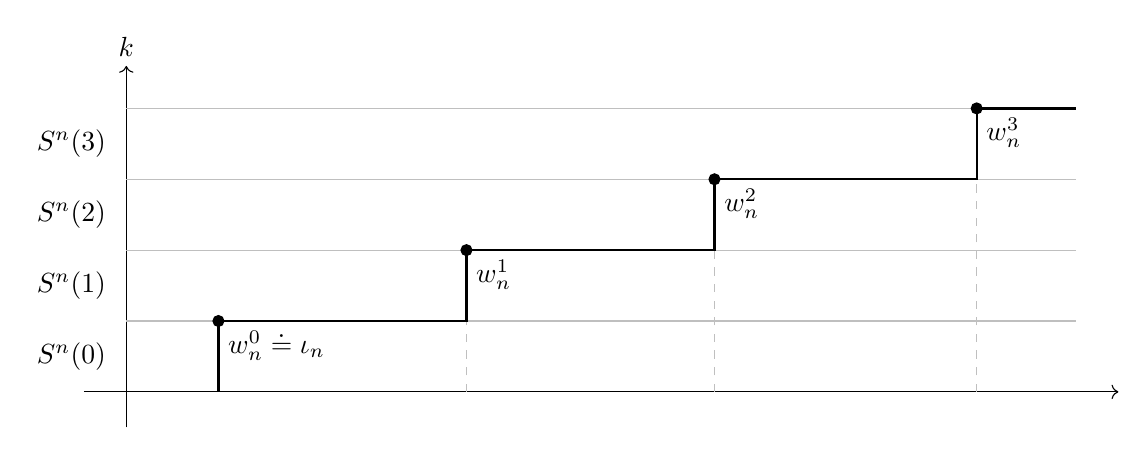
\begin{tikzpicture}[scale=0.9]

    % axes
    \draw[->] (-0.6,0) -- (14.0,0);
    \draw[->] (0,-0.5) -- (0,4.6) node[above] {$k$};

    % horizontal rows and corner classes
    \foreach \k/\y/\x/\lab in {
        0/1.0/1.3/{w_n^0 \doteq \iota_n},
        1/2.0/4.8/{w_n^1},
        2/3.0/8.3/{w_n^2},
        3/4.0/12.0/{w_n^3}
    }{
        % row
        \draw[gray!50] (0,\y) -- (13.4,\y);

        % first nontrivial class
        \filldraw[black] (\x,\y) circle (2.2pt);

        % label for corner class
        \node[below right] at (\x,\y) {$\lab$};

        % vertical guide
        \draw[dashed, gray!50] (\x,0) -- (\x,\y);
    }

    % staircase line
    \draw[thick]
        (1.3,0) --
        (1.3,1.0) --
        (4.8,1.0) --
        (4.8,2.0) --
        (8.3,2.0) --
        (8.3,3.0) --
        (12.0,3.0) --
        (12.0,4.0) --
        (13.4,4.0);

    % row labels between the horizontal lines
    \node[left] at (-0.15,0.5) {$S^n(0)$};
    \node[left] at (-0.15,1.5) {$S^n(1)$};
    \node[left] at (-0.15,2.5) {$S^n(2)$};
    \node[left] at (-0.15,3.5) {$S^n(3)$};

\end{tikzpicture}
\caption{Schematic picture of the Goodwillie spectral sequence. The Whitehead elements are represented by the corner classes, namely the first nontrivial classes in each row.}
\end{figure}

\begin{definition}
	A \emph{$k$-Whitehead element} of $S^n$ is the image of a generator under the map
	\[
	\pi_{c(n,k)}S^n(k) \longrightarrow \pi_{c(n,k)}S^n_k \cong \pi_{c(n,k)}S^n
	\]
	Any $k$-Whitehead element will be denoted by $w_n^k$.
\end{definition}

\begin{rem}
	This does not determine a unique element: any two $k$-Whitehead elements of $S^n$ differ by multiplication by a unit in $\mathbb{F}_p^\times$. Accordingly, from now on all identities involving Whitehead elements are understood up to multiplication by a unit in $\mathbb{F}_p^\times$. We write $\doteq$ to emphasize this. In particular, for $k=0$ one has $w_n^0 \doteq \iota_n$, where $\iota_n \in \pi_nS^n$ denotes the identity class.

	One could instead try to rigidify the definition by specifying a preferred generator through the cohomological description of $S^n(k)$, for instance by choosing the class corresponding to $P^{p^{k-1}n}\cdots P^n$. However, this would still require fixing the relevant cohomological identifications. In retrospect, a cleaner alternative would have been to work with the associated \emph{Whitehead group}, namely the image of $\pi_{c(n,k)}S^n(k)$ in $\pi_{c(n,k)}S^n$, which avoids this ambiguity altogether.
\end{rem}

The following lemma collects the basic properties of these elements.

\begin{lem}
	A $k$-Whitehead element $w_n^k$ satisfies:
	\begin{enumerate}
	\item (Detection) $S^n_k$ converges early if and only if $w_n^{k+1} = 0$.
	\item (Instability) $\Sigma w_n^k = 0$ when $p=2$, and $\Sigma^2 w_n^k = 0$ when $p>2$ and $n$ is odd, for $k>0$.
	\item (Order) $p \cdot w_n^k = 0$ for $k>0$.
	\end{enumerate}
\end{lem}

\begin{proof}
	We prove each statement in turn.
	\begin{enumerate}
		\item Consider the fiber sequence
		\[
		\Omega^\infty S^n(k+1) \longrightarrow S^n_{k+1} \longrightarrow S^n_k
		\]
		On $\pi_{c(n,k+1)}$ this gives an exact sequence
		\[
		\pi_{c(n,k+1)}S^n(k+1)
		\longrightarrow
		\pi_{c(n,k+1)}S^n_{k+1}
		\longrightarrow
		\pi_{c(n,k+1)}S^n_k
		\longrightarrow
		0
		\]
		Since $S^n \to S^n_{k+1}$ is an isomorphism on $\pi_{c(n,k+1)}$, we may identify the middle term with $\pi_{c(n,k+1)}S^n$. By definition, $S^n_k$ converges early if and only if the middle map is injective. This happens precisely when the first map is trivial. Since $\pi_{c(n,k+1)}S^n(k+1)$ is cyclic and its image is generated by a $(k+1)$-Whitehead element, this is equivalent to $w_n^{k+1}=0$.

		\item This follows from the commutative diagram
		% https://q.uiver.app/#q=WzAsNCxbMCwwLCJcXHBpX3tjKG4sIGspfSBTXm4oaykiXSxbMSwwLCJcXHBpX3tjKG4sIGspICsgMn1TXntuKzJ9KGspIFxcY29uZyAqIl0sWzAsMSwiXFxwaV97YyhuLCBrKX0gU15uX2siXSxbMSwxLCJcXHBpX3tjKG4sIGspICsgMn0gU157bisyfV9rIl0sWzAsMV0sWzAsMl0sWzIsMywiRV4yIiwyXSxbMSwzXV0=
		\[
		\begin{tikzcd}
			{\pi_{c(n,k)}S^n(k)} & {\pi_{c(n,k)+2}S^{n+2}(k)\cong *} \\
			{\pi_{c(n,k)}S^n_k} & {\pi_{c(n,k)+2}S^{n+2}_k}
			\arrow[from=1-1, to=1-2]
			\arrow[from=1-1, to=2-1]
			\arrow[from=1-2, to=2-2]
			\arrow["{E^2}"', from=2-1, to=2-2]
		\end{tikzcd}
		\]
		The top right group vanishes because the connectivity of $S^{n+2}(k)$ is
		\[
		c(n+2,k)= c(n,k)+2p^k>c(n,k)+2
		\]
		for $k>0$. This proves the double suspension statement, and the case $p=2$ follows similarly.

		\item For $k>0$ one has $\pi_{c(n,k)}S^n(k)\cong \mathbb{F}_p$, so every $k$-Whitehead element has order $p$. \qedhere
	\end{enumerate}
\end{proof}

We now turn to the analogous constructions for the fiber of the double suspension $W^n$.

\begin{definition}
	The approximation $W^n_k$ \emph{converges early} if the comparison map $W^n \to W^n_k$ is injective on $\pi_{c(n,k+1)}$.
\end{definition}

\begin{definition}
	A \emph{$k$-Whitehead element} of $W^n$ is the image of a generator under the map
	\[
	\pi_{c(n,k)}W^n(k) \longrightarrow \pi_{c(n,k)}W^n_k \cong \pi_{c(n,k)}W^n
	\]
	Any $k$-Whitehead element will be denoted by $\hat w_n^k$.
\end{definition}

As before, one proves the following.

\begin{lem}
	A $k$-Whitehead element $\hat w_n^k$ satisfies:
	\begin{enumerate}
		\item (Detection) $W^n_k$ converges early if and only if $\hat w_n^{k+1}=0$.
		\item (Order) $p\cdot \hat w_n^k=0$.
	\end{enumerate}
\end{lem}

The Whitehead elements for $S^n$ and for $W^n$ are related as follows.

\begin{lem}
	The canonical map $W^n \to S^n$ sends $\hat w_n^k$ to $w_n^k$, and the connecting map in the Gray sequence $\Omega^2 S^{(n+1)p-1} \to W^n$ sends $w^{k-1}_{(n+1)p-1}$ to $\hat w_n^k$. Both statements are understood up to multiplication by a unit.
\end{lem}

\begin{proof}
	The Whitehead elements are detected in the first nontrivial cohomology groups of $S^n(k)$ and $W^n(k)$, and both maps induce isomorphisms on these groups.
\end{proof}

We can now deduce the early convergence of $W^1_k$, a fact that we will need later for the computation of the homotopy groups of $S^3$.

\begin{prop}
	\label{earlyconvW}
	For $k>0$, the approximation $W^1_k$ converges early.
\end{prop}

\begin{proof}
	By the detection property, $W^1_k$ converges early if and only if $\hat w_1^{k+1}=0$. By the previous lemma, the element $\hat w_1^{k+1}$ is the image of $w^k_{2p-1}$ under the connecting map in the Gray sequence. It therefore suffices to show that $w^k_{2p-1}$ lies in the image of the Gray map
	\[
	\Omega^4 S^{2p+1} \longrightarrow \Omega^2 S^{2p-1}
	\]
	By the instability property, the element $w^k_{2p-1}$ double-suspends trivially for $k>0$. Toda's lemma \cite[lem. 2.4]{Toda3} asserts that every such element lies in the image of the Gray map. This proves that $\hat w_1^{k+1}=0$, and hence that $W^1_k$ converges early.
\end{proof}

The relationship between $w_n^k$ and $\hat w_n^k$ yields a recursive formula. If we denote by $P$ the composite
\[
\Omega^2 S^{(n+1)p-1} \to W^n \to S^n
\]
of the Gray connecting map with the canonical projection, we obtain the following.

\begin{lem}
	The Whitehead elements satisfy the recursive formula
	\[
	w_n^k \doteq P_* w^{k-1}_{(n+1)p-1} \doteq P^{(k)}_*\iota_{(n+1)p^k-1}
	\]
\end{lem}

\begin{rem}
	This recursive formula could instead be taken as the definition of the Whitehead elements, thereby avoiding the ambiguity in the choice of generators above.
\end{rem}

Note that for $p=2$, the map $P$ coincides with the $P$ map in the EHP sequence, which explains the choice of notation. The reader may verify this from our construction of the Gray sequence by iterating the EHP sequence. Moreover, it follows from the definition and the properties of the Gray map that $\Sigma^2 \circ P \simeq *$ and $P \circ p \simeq *$, thereby recovering the instability and order properties of the Whitehead elements described above. Finally, the iterate $P^{(k)}$ is a map $\Omega^{2k} S^{(n+1)p^k-1} \to S^n$, providing a topological explanation for the recurring number $c(n,k)$.

Finally, let us illustrate the recursive description with some concrete cases.

\begin{ex}
	The first Whitehead elements are:
	\begin{enumerate}
		\item $w_n^0 \doteq \iota_n \neq 0$.
		\item $w_1^k=0$ for $k>0$, since $\pi_*S^1$ is torsion-free while $w_1^k$ is torsion. Note that $w_1^1\in \pi_1S^1$ for $p=2$.
		\item $w_n^1 \doteq [\iota_n,\iota_n]$ for $p=2$. This follows from the formula $P_*\alpha=[\iota_n,\Sigma^{-n-1}\alpha]$, valid whenever the desuspension exists \cite[prop. 3.6.1]{Behrens2010}. By the Hopf invariant one theorem \cite[thm. A]{AdamsAtiyah}, this vanishes if and only if $n=1,3,7$.
		\item $w_n^1$ for $p > 2$ coincides up to a unit with the mod-$p$ Whitehead element of \cite{GrayFam,WhiteheadModp}, which is nontrivial except for $n=1$ by the Hopf invariant one theorem \cite[thm. D]{AdamsAtiyah}. This is not a Whitehead product: Whitehead products vanish on H-spaces, yet $w_3^1 \neq 0$.
		\item $w_n^k = 0$ for $p = 2$ when $k>0$ and $n=1,3,7$, since $P$ vanishes on H-spaces.
		\item $w_n^k$ for $p = 2$ is denoted by $1[j_1, \dots, j_k]$ in \cite[6.5]{Behrens2010}. In some cases, this element detects $[\iota_{j_k}, \dots, \Sigma^{-*}[\iota_{j_1}, \iota_{j_1}]]$ \cite[3.6]{Behrens2010}, but this is not always true. For instance, $w_2^2 = 1[5,2]$ is expected to detect $[\iota_2, \Sigma^{-3}[\iota_5, \iota_5]]$. However, $[\iota_5, \iota_5] \in \pi_9 S^5$ does not desuspend three times; see the metastable computations in section \ref{metastable}. In the range covered by Behrens' calculations, we observe that $w_n^k = 0$ for $k > 0$ if and only if $n = 1,3$. We also note that the element $w_4^2 = 1[9,4]$ is missing from his charts \cite[table 6.5.8, row 11]{Behrens2010}.
		\item $w_n^2 \doteq P_*[\iota_{2n+1}, \iota_{2n+1}]$ for $p = 2$. Since $P \circ 2 \simeq *$, it follows that $w_n^2 = 0$ whenever $[\iota_{2n+1}, \iota_{2n+1}]$ is divisible by $2$. This occurs when the Kervaire invariant one class $\theta_j$ exists in $\pi_{2n}\mathbb{S}$ and has order $2$; see \cite[5.2]{Kervaireexp}. This holds for $2n = 2^{j+1} - 2$ with $j \leq 6$, by the solution of the Kervaire invariant one problem \cite{Kervairesol,Kervairelast}. In particular, this implies that $w^2_{2^i - 1} = 0$ for $i \leq 6$, giving the new vanishing results $w^2_{15} = w^2_{31} = w^2_{63} = 0$.
	\end{enumerate}
\end{ex}

These examples lead naturally to the following question.

\begin{ques}
	When is $w_n^k$ nonzero?
\end{ques}

For instance, when $p=2$ one may ask whether $w_n^k \neq 0$ whenever $n$ is not of the form $2^i-1$. More generally, for fixed $k$, are infinitely many of the classes $w_n^k$ nontrivial? Does the number of vanishing classes $w_n^k$ increase with $k$? For $p>2$ and $n>1$, do any of these classes vanish? For which values of $n$ does one obtain an infinite family? We leave these questions open for further study.

\chapter{Model for the approximation circles}

The goal of this chapter is to give an explicit description of the Goodwillie approximations to $S^1$. This model will be the main input for the computations carried out later, but it is also of independent interest: it expresses $\Omega S^1_k$ in terms of well-studied spectra, namely the symmetric product spectra.

In the first part, we recall the symmetric product spectra $\mathbb{Sp}^m$ and collect some of their basic properties, including their $\mathbb{F}_p$-cohomology, their $K(i)$-cohomology, and their low-degree homotopy groups. These facts will be used repeatedly in what follows.

In the second part, we prove the central equivalence
\[
\Omega S^1_k \simeq \mathbb{Z} \times \Omega^{\infty+2k}\tau_{>0}\mathbb{Sp}^{p^k}
\]
The proof relies on the solution of the Whitehead conjecture by Behrens \cite{Behrens2011} and Kuhn \cite{Kuhn2014}. The result reduces the study of $\Omega S^1_k$ to stable homotopy theory and provides a concrete entry point for the computational applications of the next chapter.

\section{Symmetric products}

The model for $S^1_k$ will be expressed in terms of certain well-studied spectra called \textit{symmetric product spectra}. The goal of this section is to give a brief exposition of them.

The symmetric product spectra are the first derivatives of functors that go by the same name. Classically, the $m^\mathrm{th}$ symmetric product functor is defined on topological spaces by $Sp^m(X) := X^m_{\Sigma_m}$, where the product is the cartesian product and the subscript denotes strict orbits under the action of the symmetric group $\Sigma_m$.

We prefer to adopt a homotopy-invariant definition from the start. By Elmendorf's theorem \cite{Gspaces}, every $G$-space $X$ is equivalent to a functor $\mathcal{O}(G)^{\mathrm{op}} \to \mathcal{S}$ from the orbit category, sending $G/H$ to $X^H$, and strict orbits correspond to colimits of such functors. This motivates the following definition.

\begin{definition}
	The $m^\mathrm{th}$ \textit{symmetric product} is the functor $Sp^m: \mathcal{S}_* \to \mathcal{S}_*$ defined by
	\[
	Sp^mX := \mathrm{colim}_{\Sigma_m/H \in \mathcal{O}^{\mathrm{op}}(\Sigma_m)}(X^m)^H \simeq \mathrm{colim}_{\Sigma_m/H}X^{m/H}
	\]
\end{definition}

To illustrate how these colimits can be manipulated, let us work out explicitly the case $m=2$ and examine how it behaves on spheres.

\begin{ex}
	The \textit{symmetric square} is given by the functor
	\[
	Sp^2X = \mathrm{colim}_{C_2/H}X^{2/H} = \mathrm{colim}(X \to X^{2}\circlearrowleft C_2)
	\]
	where the map is the diagonal. This functor fits into a cofiber sequence
	\[
	I \longrightarrow Sp^2 \longrightarrow Sp^{\wedge 2}
	\]
	where we define $Sp^{\wedge 2}X := \mathrm{colim}(X \to X^{\wedge 2}\circlearrowleft C_2)$. Indeed, this follows by taking vertical cofibers in the diagram below.
	% https://q.uiver.app/#q=WzAsNixbMSwwLCJcXG1hdGhybXtjb2xpbX0oKiJdLFsyLDAsIlggXFx2ZWUgWCBcXGNpcmNsZWFycm93bGVmdCkiXSxbMSwxLCJcXG1hdGhybXtjb2xpbX0oWCJdLFsyLDEsIlheMiBcXGNpcmNsZWFycm93bGVmdCkiXSxbMCwwLCJJICJdLFswLDEsIlNwXjIiXSxbMCwxXSxbMCwyLCIiLDIseyJvZmZzZXQiOi01fV0sWzIsM10sWzEsMywiIiwwLHsib2Zmc2V0IjozfV0sWzQsMCwiIiwyLHsibGV2ZWwiOjIsInN0eWxlIjp7ImhlYWQiOnsibmFtZSI6Im5vbmUifX19XSxbNSwyLCIiLDIseyJsZXZlbCI6Miwic3R5bGUiOnsiaGVhZCI6eyJuYW1lIjoibm9uZSJ9fX1dLFs0LDVdXQ==
\[\begin{tikzcd}
	{I } & {\mathrm{colim}(*} & {X \vee X \circlearrowleft C_2)} \\
	{Sp^2} & {\mathrm{colim}(X} & {X^2 \circlearrowleft C_2)}
	\arrow[equals, from=1-1, to=1-2]
	\arrow[from=1-1, to=2-1]
	\arrow[from=1-2, to=1-3]
	\arrow[shift left=5, from=1-2, to=2-2]
	\arrow[shift right=3, from=1-3, to=2-3]
	\arrow[equals, from=2-1, to=2-2]
	\arrow[from=2-2, to=2-3]
\end{tikzcd}\]
	Now observe that $Sp^{\wedge 2}S^n \simeq \Sigma^n(RP^{n-1})^\diamond$. Here $\diamond$ denotes the unreduced suspension, so for $n>0$ this simplifies to $\Sigma^{n+1}RP^{n-1}$. To see this, first note that
	\[
	Sp^{\wedge 2}S^n
	=
	\mathrm{colim}(S^n \to S^{2n}\circlearrowleft C_2)
	\simeq
	\Sigma^n \mathrm{colim}(S^0 \to S^{n\rho}\circlearrowleft C_2)
	\]
	Now note that $S^{n\rho} \simeq S(n\rho)^\diamond$. Since the unreduced suspension $\diamond:\mathcal{S}\to\mathcal{S}_*$ preserves contractible colimits, and since the orbit category is contractible because it has a terminal object, it follows that
	\[
	Sp^{\wedge 2}S^n
	\simeq
	\Sigma^n \mathrm{colim}^{unpt}(\emptyset \to S(n\rho)\circlearrowleft C_2)^\diamond
	\simeq
	\Sigma^n S(n\rho)_{hC_2}^\diamond
	=
	\Sigma^n(RP^{n-1})^\diamond
	\]
	Putting everything together, we conclude that the symmetric square of a sphere fits into the cofiber sequence
	\[
	S^n \longrightarrow Sp^2S^n \longrightarrow \Sigma^n(RP^{n-1})^\diamond
	\]
\end{ex}

There are two classical results concerning symmetric products.

\begin{prop}
	The symmetric product functors satisfy:
	\begin{enumerate}
		\item $Sp^mS^1 \simeq S^1$.
		\item $Sp^\infty$ is linear.
	\end{enumerate}
\end{prop}

\begin{proof}
	The first statement is a consequence of the fundamental theorem of algebra; see, for instance, \cite[lem. 7.10]{AroneDwyer}. The second is the content of the Dold--Thom theorem \cite{doldthom}.
\end{proof}

Combining these results, we deduce that $Sp^\infty \simeq \Omega^\infty(\mathbb{Z} \otimes -)$. In particular, we obtain the following filtration of the Hurewicz map:
\[
I = Sp^1
\longrightarrow \cdots
\longrightarrow Sp^{m-1}
\longrightarrow Sp^m
\longrightarrow \cdots
\longrightarrow Sp^\infty \simeq \Omega^\infty(\mathbb{Z} \otimes -)
\]

We are now ready to define the symmetric product spectra as the first derivatives of the symmetric product functors.

\begin{definition}
	\label{symmprod}
	The $m^\mathrm{th}$ \textit{symmetric product spectrum} is defined by
	\[
	\mathbb{Sp}^m := \partial_1 Sp^m
	\]
\end{definition}

\begin{lem}
	There is an equivalence
	\[
	\mathbb{Sp}^m \simeq \mathrm{colim}_{\Sigma_m/H} \mathbb{S}^{\oplus m/H}
	\]
\end{lem}

\begin{proof}
	By the definition of $Sp^m$, and since $\partial_1$ preserves colimits of reduced functors, we have
	\[
	\mathbb{Sp}^m
	= \partial_1 Sp^m
	= \partial_1 \mathrm{colim}_{\Sigma_m/H}(-)^{m/H}
	\simeq \mathrm{colim}_{\Sigma_m/H} \partial_1\bigl((-)^{m/H}\bigr)
	\]
	On the other hand, for every finite set $A$ one has
	\[
	\partial_1\bigl((-)^A\bigr) \simeq \mathbb{S}^{\oplus A}
	\]
	Hence the claim follows.
\end{proof}

\begin{rem}
	Here and below we use that $\partial_1$ preserves colimits of reduced functors. Indeed, for a reduced functor $F$ one has
	\[
	\partial_1F \simeq \mathrm{colim}_n \Sigma^{-n}\Sigma^\infty F(S^n)
	\]
	so $\partial_1$ is given by a colimit-preserving construction.
\end{rem}

An alternative description, due to Lesh \cite{ktheorymult} but not needed here, is that $\mathbb{Sp}^m$ can be identified with the algebraic $K$-theory of the category of multisets with multiplicity at most $m$.

\begin{ex}
	\label{reducedtransfer}
	For $m=2$, the previous discussion gives the cofiber sequence
	\[
	\mathbb{S} \longrightarrow \mathbb{Sp}^2 \longrightarrow \Sigma\mathbb{RP}^\infty
	\]
	This follows by applying $\partial_1$ to the cofiber sequence $I \to Sp^2 \to Sp^{\wedge 2}$ and using the fact that $Sp^{\wedge 2}S^n \simeq \Sigma^{n+1}RP^{n-1}$ for $n>0$.

	Moreover, the map $\mathbb{RP}^\infty \to \mathbb{S}$ obtained by rotating this sequence is the classical Kahn--Priddy map \cite{KP,KPWelcher}.
\end{ex}

From now on, we will no longer use the functors $Sp^m$, but only their first derivatives $\mathbb{Sp}^m$. Before leaving the functors behind, however, it is natural to ask the following question.

\begin{ques}
	What do the higher Goodwillie approximations of $Sp^m$ look like?
\end{ques}

By taking $\partial_1$ of the filtration above, we obtain the sequence of symmetric product spectra
\[
\mathbb{S} \simeq \mathbb{Sp}^1
\longrightarrow \cdots
\longrightarrow \mathbb{Sp}^{m-1}
\longrightarrow \mathbb{Sp}^m
\longrightarrow \cdots
\longrightarrow \mathbb{Sp}^\infty \simeq \mathbb{Z}
\]
This sequence is an equivalence on $\pi_0\cong\mathbb{Z}$. The original \emph{Whitehead conjecture} asks whether these maps are null on $\pi_*$ for $*>0$, a question answered affirmatively by Kuhn \cite{WhiteheadOriginal}.

More generally, we can consider the quotients of this filtration. First, note that at the functor level
\[
Sp^m/Sp^{m-1} \simeq Sp^{\wedge m} := \mathrm{colim}_{\Sigma_m/H}(-)^{\wedge m/H}
\]
Applying $\partial_1$, we obtain
\[
\mathbb{Sp}^m/\mathbb{Sp}^{m-1}
\simeq \partial_1Sp^{\wedge m}
\simeq \mathrm{colim}_{\Sigma_m/H}
\begin{cases}
\mathbb{S} & \text{if } m/H = 1 \\
* & \text{if } m/H \neq 1
\end{cases}
\simeq \Sigma^{\infty+\diamond}\mathrm{colim}_{\Sigma_m/H}^{unpt}
\begin{cases}
\emptyset & \text{if } m/H = 1 \\
* & \text{if } m/H \neq 1
\end{cases}
\]
This recovers Lesh's result \cite{nontransitive}:
\[
\mathbb{Sp}^m/\mathbb{Sp}^{m-1} \simeq \Sigma^{\infty+\diamond} B_{nt}\Sigma_m
\]
where $B_{nt}\Sigma_m$ is the classifying space of the family of non-transitive subgroups of $\Sigma_m$. It also recovers the calculation for $m=2$ from example \ref{reducedtransfer}, since $B_{nt}\Sigma_2 = B\Sigma_2 = RP^\infty$.

These quotients behave in a way reminiscent of the Goodwillie tower of the identity after $p$-localization: they are trivial unless $m=p^k$. Indeed, after $p$-localization, a standard transfer argument \cite[sec. 7]{nontransitive} allows us to compute the above colimit using only those orbits $\Sigma_m/H$ for which $H$ is a $p$-subgroup; if $m$ is not a power of $p$, none of these subgroups can act transitively on $m$ letters, and the colimit becomes contractible. Consequently, we only need to focus on the spectra $\mathbb{Sp}^{p^k}$.

The spectra $\mathbb{Sp}^{p^k}$ are well studied. Their $\mathbb{F}_p$-cohomology and $K(i)$-cohomology are completely understood.

To describe their $\mathbb{F}_p$-cohomology, recall from the previous chapter, before proposition \ref{cohomS}, the $\mathcal{A}$-module $(\mathcal{A}/\mathcal{A}\beta)_{\geq k}$ defined by the length filtration on $\mathcal{A}/\mathcal{A}\beta$. The following computation goes back to Nakaoka \cite{Nakaoka}, who showed that the map $\mathbb{Sp}^{p^k} \to \mathbb{Z}$ induces a surjection
\[
\mathcal{A}/\mathcal{A}\beta \cong \mathbb{F}_p^*\mathbb{Z} \twoheadrightarrow \mathbb{F}_p^*\mathbb{Sp}^{p^k}
\]
with kernel $(\mathcal{A}/\mathcal{A}\beta)_{\geq k+1}$. A more direct reference for the formulation below is \cite[thm. 4.1]{MitchellPriddy}.

\begin{prop}
	\label{symmprodfp}
	The $\mathbb{F}_p$-cohomology of the symmetric product spectra is given by
	\begin{align*}
		\mathbb{F}_p^*\mathbb{Sp}^{p^k}
		&\cong (\mathcal{A}/\mathcal{A}\beta)_{\leq k}
		:= (\mathcal{A}/\mathcal{A}\beta)/(\mathcal{A}/\mathcal{A}\beta)_{\geq k+1} \\
		&= \mathbb{F}_p\bigl\langle \theta^I \in \mathcal{A}/\mathcal{A}\beta \mid I \text{ admissible of length } \leq k \bigr\rangle
	\end{align*}
\end{prop}

\begin{rem}
	It is worth noting that the previous calculation shows that
	\[
	\mathbb{F}_p^*\tau_{>0}\mathbb{Sp}^{p^k}
	\cong
	\Sigma^{-1}(\mathcal{A}/\mathcal{A}\beta)_{\geq k+1}
	\]
	In this sense, both from this calculation and from the next result, as well as from the model itself, the connected symmetric product spectra appear to be more natural objects than the non-connected ones.
\end{rem}

From this cohomological information, one can run an Adams spectral sequence to compute the homotopy groups. For fixed $k$, computer calculations can produce charts over a large range; examples will appear in later sections, and an implementation for the approximation circles is available in \cite{NervoCircle}. Here we record the general pattern of the first few nontrivial groups, which will suffice for our purposes.

\begin{lem}
	\label{homotopysp}
    The first three nontrivial homotopy groups of the symmetric product spectra are given by
    \[
    \pi_*\mathbb{Sp}^{p^k} \cong
    \begin{cases}
        \mathbb{Z} & * = 0 \\
        \mathbb{F}_p & * = 2(p^{k+1}-1)-1 \\
		\mathbb{F}_p & * = N(p^{k+1}-1)-1 \\
        0 & * \leq N(p^{k+1}-1)-1, \text{otherwise}
    \end{cases}
    \]
	where $N=3$ if $p=2$ and $N=4$ if $p>2$.
\end{lem}

\begin{proof}
	We already know that there is a copy of $\mathbb{Z}$ in degree $0$, and that
	\[
	\mathbb{F}_p^*\tau_{>0}\mathbb{Sp}^{p^k}
	\cong
	\Sigma^{-1}(\mathcal{A}/\mathcal{A}\beta)_{\geq k+1}
	\]
	The first nontrivial element in this cohomology is $M_{k+1} := P^{p^k}\cdots P^pP^1$ in degree $d := 2(p^{k+1}-1)$. This has a nontrivial Bockstein, namely the element $\beta P^{p^k}\cdots P^pP^1$, and hence gives a copy of $\mathbb{F}_p$ in degree $d-1$, because of the shift. Next, consider the fiber sequence
	\[
	\tau_{>d-1}\mathbb{Sp}^{p^k}
	\longrightarrow
	\tau_{>0}\mathbb{Sp}^{p^k}
	\longrightarrow
	\Sigma^{d-1}\mathbb{F}_p
	\]
	This induces the following long exact sequence in $\mathbb{F}_p$-cohomology:
	\[
	\cdots
	\longrightarrow
	\mathbb{F}_p^{*+d-2}\tau_{>d-1}\mathbb{Sp}^{p^k}
	\longrightarrow
	\mathcal{A}^*
	\xlongrightarrow{\cdot M_{k+1}}
	((\mathcal{A}/\mathcal{A}\beta)_{\geq k+1})^{*+d}
	\longrightarrow
	\cdots
	\]
	The next nontrivial homotopy group appears exactly where right multiplication by $M_{k+1}$ ceases to be an isomorphism. Equivalently, this amounts to studying right multiplication by $M_{k+1}\beta$ as a map
	\[
	\mathcal{A}^*
	\longrightarrow
	(\mathcal{A}_{\geq k+1}\beta)^{*+d+1}
	\]
	This analysis is carried out in the appendix (lem. \ref{mult2} and lem. \ref{multodd}). There we show that this map is an isomorphism for $*<e$, and that it has kernel $\mathbb{F}_p$ in degree $e$, where $e=2^{k+1}$ if $p=2$ and $e=2p^{k+1}-1$ if $p>2$. This implies that the next nontrivial homotopy group is in degree $d-2+e$. To conclude, note that $e-1=M(p^{k+1}-1)$, where $M=1$ if $p=2$ and $M=2$ if $p>2$, and so $d-2+e=(M+2)(p^{k+1}-1)-1$.
\end{proof}

The proof above is somewhat indirect. It would be more elegant to write down explicitly the beginning of a minimal resolution of the cohomology.

\begin{ques}
	What does the beginning of a minimal resolution of the module $(\mathcal{A}/\mathcal{A}\beta)_{\geq k+1}$ look like?
\end{ques}

Besides their $\mathbb{F}_p$-cohomology, the $K(i)$-cohomology of the symmetric product spectra can also be described; we learned this from a private communication with Nick Kuhn. We will only need this for $i\leq k+1$.

\begin{prop}
	\label{symmprodkn}
	The symmetric product spectrum $\mathbb{Sp}^{p^k}$ is $K(i)$-acyclic for $0 < i \leq k$, and its $K(k+1)$-cohomology has rank $p^{\binom{k+1}{2}}$ over $K(k+1)_*$.
\end{prop}

\begin{proof}
	The first statement is due to Welcher \cite[thm. 5.1]{Welcher}. Starting from Nakaoka's calculation, he showed that the $\mathbb{F}_p$-cohomology of $\tau_{>0}\mathbb{Sp}^{p^k}$, which he calls the \textit{symmetric fibers}, is free over the subalgebra $\mathcal{A}(k)$. This freeness implies that its Adams spectral sequence has a vanishing line of slope smaller than $1/|v_i|$ for $i\leq k$, and hence that it is $K(i)$-acyclic in this range. For the non-connected version, the difference is a copy of $\mathbb{Z}$, which is $K(i)$-acyclic only for $i>0$.
	
	The second statement follows from the first together with a result of Kuhn \cite[ex. 6.5]{Spchrom}. Consider the sequence
	\[
	\mathbb{Sp}^{p^k}
	\longrightarrow
	\mathbb{Sp}^{p^{k+1}}
	\longrightarrow
	\mathbb{Sp}^{p^{k+1}}/\mathbb{Sp}^{p^k}
	=: \Sigma^{k+1}L(k+1)
	\]
	By the first part, the boundary map $\Sigma^kL(k+1) \to \mathbb{Sp}^{p^k}$ is a $K(k+1)$-equivalence. Kuhn's result then tells us that the $K(n)$-cohomology of $L(n)$ has rank $p^{\binom{n}{2}}$, which gives the desired claim.
\end{proof}

\begin{rem}
	It is worth emphasizing again that this statement about cohomology is cleaner for the connected symmetric product spectrum $\tau_{>0}\mathbb{Sp}^{p^k}$, as we saw in the proof.
\end{rem}

Since the first nontrivial height appears at $k+1$, it is natural to ask the following question.

\begin{ques}
	Can we give an explicit computation of $\pi_*L_{K(k+1)}\mathbb{Sp}^{p^k}$, analogous to the known case $k = 0$?
\end{ques}

We conclude this section by making the connection between symmetric products and the Goodwillie tower of $S^1$ explicit. Nakaoka's calculation shows that the $\mathbb{F}_p$-cohomology of the quotient $\mathbb{Sp}^{p^k}/\mathbb{Sp}^{p^{k-1}}$ is given by the $\mathcal{A}$-module $(\mathcal{A}/\mathcal{A}\beta)_{=k}$. Up to a suspension shift, this coincides with the cohomology of the layer $S^1(k)$ computed by Arone--Mahowald. Remarkably, Arone--Dwyer lifted this to an equivalence of spectra.

\begin{prop}[{\cite[thm. 1.18]{AroneDwyer}}]
	\label{aronedwyer}
	There is an equivalence of spectra
	\[
	S^1(k) \simeq \Sigma^{1-2k}\mathbb{Sp}^{p^k}/\mathbb{Sp}^{p^{k-1}}
	\]
\end{prop}

\section{The model}

We are now ready to state and prove the main theorem of this thesis.

\begin{thm}[Model for the approximation circles]
	\label{model}
	There is an equivalence
	\[
	\Omega S^1_k \simeq \mathbb{Z} \times \Omega^{\infty+2k}\tau_{>0}\mathbb{Sp}^{p^k}
	\]
\end{thm}

\begin{rem}
	Since $\tau_{>0}\mathbb{Sp}^m$ is rationally trivial, and since the maps $P_mI(S^1) \to P_{p^k}I(S^1)$ and $\tau_{>0}\mathbb{Sp}^{p^k} \to \tau_{>0}\mathbb{Sp}^m$ are $p$-local equivalences whenever $p^k \leq m < p^{k+1}$, a fracture square argument upgrades the result above to an integral equivalence
	\[
	\Omega P_mI(S^1) \simeq \mathbb{Z} \times \textstyle\prod_p\Omega^{\infty+2\lfloor\log_pm\rfloor}\bigl(\tau_{>0}\mathbb{Sp}^m\bigr)^\wedge_p
	\]
	We will not use this expression in what follows. It is nevertheless amusing to observe that the $m^\mathrm{th}$ stage of the Goodwillie tower of $S^1$ is determined by the spectrum $\mathbb{Sp}^m$, though not in a straightforward way. Rather, the spectrum is disassembled, shifted according to the arithmetic of $m$, and then reassembled.
\end{rem}

The proof proceeds in three steps. First, for a general functor $F$ we define the \emph{$m^\mathrm{th}$ remainder} $R_mF$ to be the fiber of the map $F \to P_mF$. We then show that $\Omega S^1_k \simeq \mathbb{Z} \times R_{p^k}I(S^1)$. Second, we construct maps between $R_{p^k}I(S^1)$ and $\Omega^{\infty+2k}\tau_{>0}\mathbb{Sp}^{p^k}$ using Arone--Dwyer's equivalence above. Finally, we prove that these maps are equivalences by appealing to the calculus version of the Whitehead conjecture, as resolved by Behrens \cite{Behrens2011} and Kuhn \cite{Kuhn2014}.

We start with a basic lemma about sections and splittings.

\begin{lem}[Splitting lemma]
	\label{splittinglemma}
    If the composite $X \to Y \to X$ is an equivalence, then
    \begin{enumerate}
        \item $\mathrm{fib}(X \to Y) \simeq \Omega \mathrm{fib}(Y \to X)$
        \item $\Omega Y \simeq \Omega X \times \Omega\mathrm{fib}(Y \to X)$
        \item $\Omega Y \simeq \Omega X \times \mathrm{fib}(X \to Y)$
    \end{enumerate}
\end{lem}

\begin{proof}
    The third statement follows immediately from the first two, so it suffices to prove the first two. Since the composite $X \to Y \to X$ is an equivalence, its fiber is contractible. By iterating pullbacks, we obtain the diagram

    % https://q.uiver.app/#q=WzAsNixbMCwxLCJYIl0sWzAsMCwiKiJdLFsxLDEsIlkiXSxbMSwwLCJcXG1hdGhybXtmaWJ9KFkgXFx0byBYKSJdLFsyLDEsIlgiXSxbMiwwLCIqIl0sWzEsMF0sWzAsMl0sWzEsM10sWzMsMl0sWzIsNF0sWzMsNV0sWzUsNF0sWzMsNCwiIiwxLHsic3R5bGUiOnsibmFtZSI6ImNvcm5lciJ9fV0sWzEsMiwiIiwxLHsic3R5bGUiOnsibmFtZSI6ImNvcm5lciJ9fV1d
\[
\begin{tikzcd}
	{*} & {\mathrm{fib}(Y \to X)} & {*} \\
	X & Y & X
	\arrow[from=1-1, to=1-2]
	\arrow[from=1-1, to=2-1]
	\arrow["\lrcorner"{anchor=center, pos=0.125}, draw=none, from=1-1, to=2-2]
	\arrow[from=1-2, to=1-3]
	\arrow[from=1-2, to=2-2]
	\arrow["\lrcorner"{anchor=center, pos=0.125}, draw=none, from=1-2, to=2-3]
	\arrow[from=1-3, to=2-3]
	\arrow[from=2-1, to=2-2]
	\arrow[from=2-2, to=2-3]
\end{tikzcd}
\]
    Both statements now follow from the fact that the left square is a pullback. Indeed, the first follows by taking horizontal fibers of the left square, while the second follows by rotating the induced fiber sequence
    \[
        \Omega Y \longrightarrow * \longrightarrow X \times \mathrm{fib}(Y \to X)
    \qedhere
    \]
\end{proof}

The previous lemma immediately gives the desired splitting. The point is that $S^1$ is already detected by its stable approximation, and hence by every further approximation.

\begin{lem}
    $\Omega S^1_k \simeq \mathbb{Z} \times R_{p^k}I(S^1)$.
\end{lem}

\begin{proof}
    By part (3) of the previous lemma, it suffices to show that the comparison map $S^1 \to S^1_k$ admits a retraction. Consider the composite
    \[
        S^1_k \longrightarrow S^1_0 \simeq \Omega^\infty \mathbb{S}^1 \longrightarrow \Omega^\infty\Sigma \mathbb{Z} \simeq S^1
    \]
    where the second map is induced by the suspension of the unit map $\mathbb{S} \to \mathbb{Z}$. The resulting composite $S^1 \to S^1_k \to S^1$ factors as $S^1 \to S^1_0 \to S^1$. The first map is the stabilization map, while the second is induced by the suspension of $\mathbb{S} \to \mathbb{Z}$, so both induce isomorphisms on $\pi_1$. Since $\pi_1$ is the only nontrivial homotopy group of $S^1$, it follows that the composite is an equivalence. Thus $S^1_k \to S^1$ is a retraction, and the claim follows.
\end{proof}

\begin{rem}
	\label{remisloop}
    The retraction constructed in the proof also shows that $R_{p^k}I(S^1)$ is a loop space. Indeed, by part (1) of the splitting lemma, it identifies with the loop space of the fiber of the retraction $S^1_k \to S^1$. We will use this later in the proof of the model.
\end{rem}

\begin{rem}
	\label{retractioninfloop}
	This holds more generally for every infinite loop space $\Omega^\infty X$. In particular, it also holds for $S^0$. Indeed, a retraction of the map $\Omega^\infty X \to P_mI(\Omega^\infty X)$ is given by the composite
	\[
	P_mI(\Omega^\infty X)
	\longrightarrow
	P_1I(\Omega^\infty X)
	\simeq
	\Omega^\infty \Sigma^\infty \Omega^\infty X
	\xlongrightarrow{\Omega^\infty\epsilon}
	\Omega^\infty X
	\]
	where $\epsilon$ is the counit of the adjunction $\Sigma^\infty \dashv \Omega^\infty$. This is indeed a retraction by the triangle identities.
\end{rem}

\begin{rem}
	\label{noretractionnocry}
	On the other hand, if $X$ is a simply connected finite non-contractible space, then the map $X \to P_mI(X)$ never admits a retraction, not even after looping sufficiently many times. In particular, no spheres other than $S^0$ and $S^1$ admit such a retraction.
	
	To see this, suppose there exist $m$ and $h$ together with a retraction
	\[
	\Omega^h P_mI(X) \xlongrightarrow{r} \Omega^h X
	\]
	Choose $m$ minimal with this property. We will prove that $m=0$, so that $\Omega^hX \simeq *$. This implies $X \simeq *$, since every simply connected finite space other than the point has infinitely many nontrivial homotopy groups, by an old result of Serre \cite[thm. 10]{Serre}.

	Suppose now that $m>0$. By Levy's spectral Sullivan conjecture \cite[thm. 1.1]{spectralSullivan}, the composite
	\[
	\Omega^{\infty+h}\mathbb{D}_mI(X)
	\longrightarrow
	\Omega^hP_mI(X)
	\xlongrightarrow{r}
	\Omega^hX
	\]
	factors through the $1$-truncation of the source. In particular, after looping twice, the map
	\[
	\Omega^{\infty+h+2}\mathbb{D}_mI(X)
	\longrightarrow
	\Omega^{h+2}P_mI(X)
	\xlongrightarrow{\Omega^2r}
	\Omega^{h+2}X
	\]
	is null. Hence we obtain a factorization
	\[
	\Omega^{\infty+h+2}\mathbb{D}_mI(X)
	\longrightarrow
	\Omega^2\mathrm{fib}(r)
	\longrightarrow
	\Omega^{h+2}P_mI(X)
	\]
	The fiber of this composite is described by the following pullback diagram:
	% https://q.uiver.app/#q=WzAsNixbMCwxLCJcXE9tZWdhXntcXGluZnR5ICsgaCArIDJ9XFxtYXRoYmJ7RH1fbUkoWCkiXSxbMSwxLCJcXE9tZWdhXjJcXG1hdGhybXtmaWJ9KHIpIl0sWzIsMSwiXFxPbWVnYV57aCsyfVBfbUkoWCkiXSxbMiwwLCIqIl0sWzAsMCwiXFxPbWVnYV57aCszfVBfe20tMX1JKFgpIl0sWzEsMCwiXFxPbWVnYV57aCszfVgiXSxbMCwxXSxbMSwyLCIiLDAseyJzdHlsZSI6eyJ0YWlsIjp7Im5hbWUiOiJob29rIiwic2lkZSI6InRvcCJ9fX1dLFszLDJdLFs0LDBdLFs1LDNdLFs0LDVdLFs1LDEsIioiLDFdLFs1LDIsIiIsMSx7InN0eWxlIjp7Im5hbWUiOiJjb3JuZXIifX1dLFs0LDEsIiIsMSx7InN0eWxlIjp7Im5hbWUiOiJjb3JuZXIifX1dXQ==
\[\begin{tikzcd}
	{\Omega^{h+3}P_{m-1}I(X)} & {\Omega^{h+3}X} & {*} \\
	{\Omega^{\infty + h + 2}\mathbb{D}_mI(X)} & {\Omega^2\mathrm{fib}(r)} & {\Omega^{h+2}P_mI(X)}
	\arrow[from=1-1, to=1-2]
	\arrow[from=1-1, to=2-1]
	\arrow["\lrcorner"{anchor=center, pos=0.125}, draw=none, from=1-1, to=2-2]
	\arrow[from=1-2, to=1-3]
	\arrow["{*}"{description}, from=1-2, to=2-2]
	\arrow["\lrcorner"{anchor=center, pos=0.125}, draw=none, from=1-2, to=2-3]
	\arrow[from=1-3, to=2-3]
	\arrow[from=2-1, to=2-2]
	\arrow[hook, from=2-2, to=2-3]
\end{tikzcd}\]
	which shows that $\Omega^{h+3}X$ is a retract of $\Omega^{h+3}P_{m-1}I(X)$, contradicting the minimality of $m$.
	
	This phenomenon is not specific to the Goodwillie tower, but holds for any finite extension of infinite loop spaces. It probably deserves to be stated as a lemma, but we prefer not to distract the reader from the main line of the argument.
\end{rem}

The rest of this section is devoted to proving the equivalence
\[
R_{p^k}I(S^1) \simeq \Omega^{\infty+2k}\tau_{>0}\mathbb{Sp}^{p^k}
\]
The first step is to produce maps between these spaces. The guiding idea is that, by the work of Arone--Dwyer, both sides come equipped with filtrations whose associated graded pieces are the same.

Indeed, the remainder $R_mF$ has the same associated graded as the Goodwillie tower, up to a shift, as the following lemma shows.

\begin{lem}
    If $F$ is a reduced functor, there are fiber sequences $R_mF \to R_{m-1}F \to D_mF$.
\end{lem}

\begin{proof}
    This follows by taking vertical fibers of the diagram
    % https://q.uiver.app/#q=WzAsNixbMCwwLCJGIl0sWzAsMSwiUF9tRiJdLFsxLDAsIkYiXSxbMiwwLCIqIl0sWzIsMSwiQkRfbUYiXSxbMSwxLCJQX3ttLTF9RiJdLFswLDFdLFswLDIsIiIsMix7ImxldmVsIjoyLCJzdHlsZSI6eyJoZWFkIjp7Im5hbWUiOiJub25lIn19fV0sWzIsM10sWzMsNF0sWzIsNV0sWzEsNV0sWzUsNF1d
\[\begin{tikzcd}
	F & F & {*} \\
	{P_mF} & {P_{m-1}F} & {BD_mF}
	\arrow[equals, from=1-1, to=1-2]
	\arrow[from=1-1, to=2-1]
	\arrow[from=1-2, to=1-3]
	\arrow[from=1-2, to=2-2]
	\arrow[from=1-3, to=2-3]
	\arrow[from=2-1, to=2-2]
	\arrow[from=2-2, to=2-3]
\end{tikzcd}\]
    The existence of a delooping of derivatives for reduced functors is a standard result in calculus \cite[lem. 2.2]{GoodwillieIII}.
\end{proof}

In particular, applying this to the identity functor, evaluating at $S^1$, and using proposition \ref{aronedwyer}, we obtain fiber sequences
\[
R_{p^k}I(S^1)
\longrightarrow
R_{p^{k-1}}I(S^1)
\longrightarrow
\Omega^\infty S^1(k)
\simeq
\Omega^{\infty-1+2k}\mathbb{Sp}^{p^k}/\mathbb{Sp}^{p^{k-1}}
\]
On the other hand, since $\mathbb{Sp}^{p^k}/\mathbb{Sp}^{p^{k-1}}$ is connected, taking connected covers gives fiber sequences
\[
\tau_{>0}\mathbb{Sp}^{p^{k-1}}
\longrightarrow
\tau_{>0}\mathbb{Sp}^{p^k}
\longrightarrow
\mathbb{Sp}^{p^k}/\mathbb{Sp}^{p^{k-1}}
\]
Before using these fiber sequences to construct the maps and prove the general result, we give a direct proof in the case $p=2$ and $k\leq 1$.

\begin{ex}
	\label{remainder0}
	We first identify the case $k=0$. We claim that
	\[
	R_1I(S^1) \simeq \Omega^\infty\tau_{>0}\mathbb{S}
	\]
	Indeed, by part (1) of the splitting lemma (lem. \ref{splittinglemma}), it suffices to identify the fiber of the retraction $S^1_0 \to S^1$. Such a retraction is given by applying $\Omega^\infty$ to the shifted unit map $\mathbb{S}^1 \to \Sigma\mathbb{Z}$. Its fiber is $\Sigma\tau_{>0}\mathbb{S}$, and the claim follows.
\end{ex}

\begin{ex}
	\label{remainder1}
	We now identify the case $k=1$, namely
	\[
	R_2I(S^1) \simeq \Omega^{\infty+2}\tau_{>0}\mathbb{Sp}^2
	\]
	By the previous example and the previous lemma, there is a fiber sequence
	\[
	R_2I(S^1)
	\longrightarrow
	R_1I(S^1) \simeq \Omega^\infty\tau_{>0}\mathbb{S}
	\xlongrightarrow{\delta}
	\Omega^\infty S^1(1) \simeq \Omega^\infty\mathbb{RP}^\infty
	\]
	On the other hand, the symmetric product spectra fit into a fiber sequence
	\[
	\mathbb{RP}^\infty
	\simeq
	\Sigma^{-1}(\mathbb{Sp}^2/\mathbb{S})
	\xlongrightarrow{\mu}
	\tau_{>0}\mathbb{S}
	\longrightarrow
	\tau_{>0}\mathbb{Sp}^2
	\]
	where the first map is the reduced Kahn--Priddy map. By the reduced Kahn--Priddy theorem, the composite
	\[
	\Omega^\infty\tau_{>0}\mathbb{S}
	\xlongrightarrow{\delta}
	\Omega^\infty\mathbb{RP}^\infty
	\xlongrightarrow{\Omega^\infty \mu}
	\Omega^\infty\tau_{>0}\mathbb{S}
	\]
	is an equivalence. Applying part (1) of the splitting lemma (lem. \ref{splittinglemma}), we conclude that
	\[
	R_2I(S^1)
	\simeq
	\Omega^{\infty+1}\mathrm{fib}(\mu)
	\simeq
	\Omega^{\infty+2}\tau_{>0}\mathbb{Sp}^2
	\]
	This is the example that motivated the whole thesis. The reader may compare it with lemma \ref{modelS1P2}, which contains the original motivating example in the metastable category.
\end{ex}

\begin{rem}
	These examples can be generalized to all infinite loop spaces $\Omega^\infty X$, thanks to Kuhn's generalized Kahn--Priddy theorem \cite[thm. 1.1]{genKP}. First, note from remark \ref{retractioninfloop} and part (1) of the splitting lemma (lem. \ref{splittinglemma}) that
	\[
	R_1I(\Omega^\infty X) \simeq \Omega^{\infty+1}\mathrm{fib}(\epsilon) \simeq \Omega^{\infty+1}\mathrm{fib}(\Sigma^\infty \Omega^\infty X \to X)
	\]
	where $\epsilon$ is the counit of the adjunction $\Sigma^\infty \dashv \Omega^\infty$. Hence, by the previous lemma, the remainder fits into a fiber sequence
	\[
	R_2I(\Omega^\infty X)
	\longrightarrow
	R_1I(\Omega^\infty X)
	\simeq
	\Omega^{\infty+1}\mathrm{fib}(\epsilon)
	\xlongrightarrow{\delta}
	D_2I(\Omega^\infty X)
	\simeq
	\Omega^{\infty+1}(\Sigma^\infty\Omega^\infty X)^{\otimes 2}_{hC_2}
	\]
	On the other hand, Kuhn \cite[thm. 1.1]{genKP} shows that the multiplication map
	\[
	(\Sigma^\infty\Omega^\infty X)^{\otimes 2}_{hC_2}
	\longrightarrow
	\Sigma^\infty\Omega^\infty X
	\]
	factors as
	\[
	(\Sigma^\infty\Omega^\infty X)^{\otimes 2}_{hC_2}
	\xlongrightarrow{\mu}
	\mathrm{fib}(\epsilon)
	\longrightarrow
	\Sigma^\infty\Omega^\infty X
	\]
	and that $\Omega^{\infty+1}\mu$ provides a retraction to the map $\delta$ above. Applying part (1) of the splitting lemma, we conclude that
	\[
	R_2I(\Omega^\infty X) \simeq \Omega^{\infty+2}\mathrm{fib}(\mu)
	\]
	This assembles into an equivalence
	\[
	\Omega P_2I(\Omega^\infty X)
	\simeq
	\Omega^{\infty+1}X \times \Omega^{\infty+2}\mathrm{fib}(\mu) \simeq \Omega^{\infty+1}X \times \Omega^{\infty+2} \mathrm{tfib} \left(
		\begin{tikzcd}[cramped, sep=small]
		(\Sigma^\infty\Omega^\infty X)^{\otimes 2}_{hC_2} \arrow[r] \arrow[d] & \Sigma^\infty\Omega^\infty X \arrow[d] \\
		* \arrow[r] & X
		\end{tikzcd}
	\right)
	\]
	We believe that this behaviour generalizes to the whole Goodwillie tower, but we were unable to prove it, so we leave it as a question.
\end{rem}

\begin{ques}
	Is $\Omega P_mI(\Omega^\infty X)$ always an infinite loop space?
\end{ques}

\begin{rem}
	On the other hand, if $X$ is a simply connected finite non-contractible space, then the remainder $R_mI(X)$ cannot be an infinite loop space. Indeed, if it were, the map $R_mI(X) \to X$ would be null, since by Levy's spectral Sullivan conjecture \cite[thm. 1.1]{spectralSullivan} it would factor through the $1$-truncation of $R_mI(X)$. Hence $\Omega X$ would be a retract of $\Omega P_mI(X)$, and we saw in remark \ref{noretractionnocry} that this is impossible.
\end{rem}

To construct the maps, consider the rotations of the fiber sequences above:
\[
\Omega^{\infty+1}S^1(k)
\longrightarrow
R_{p^k}I(S^1)
\longrightarrow
R_{p^{k-1}}I(S^1)
\longrightarrow
\Omega^\infty S^1(k)
\]
\[
\Sigma^{-1}\mathbb{Sp}^{p^k}/\mathbb{Sp}^{p^{k-1}}
\longrightarrow
\tau_{>0}\mathbb{Sp}^{p^{k-1}}
\longrightarrow
\tau_{>0}\mathbb{Sp}^{p^k}
\longrightarrow
\mathbb{Sp}^{p^k}/\mathbb{Sp}^{p^{k-1}}
\]
Using these, together with Arone--Dwyer's equivalence (prop. \ref{aronedwyer})
\[
S^1(k) \simeq \Sigma^{1-2k}\mathbb{Sp}^{p^k}/\mathbb{Sp}^{p^{k-1}}
\]
we obtain two maps
\[
R_{p^k}I(S^1)
\longrightarrow
\Omega^\infty S^1(k+1)
\simeq
\Omega^{\infty+2k+1}\mathbb{Sp}^{p^{k+1}}/\mathbb{Sp}^{p^k}
\longrightarrow
\Omega^{\infty+2k}\tau_{>0}\mathbb{Sp}^{p^k}
\]
\[
\Omega^{\infty+2k}\tau_{>0}\mathbb{Sp}^{p^k}
\longrightarrow
\Omega^{\infty+2k}\mathbb{Sp}^{p^k}/\mathbb{Sp}^{p^{k-1}}
\simeq
\Omega^{\infty+1}S^1(k)
\longrightarrow
R_{p^k}I(S^1)
\]
We will prove that these maps are equivalences by showing that their composites are equivalences. These composites are
\[
R_{p^k}I(S^1)
\longrightarrow
\Omega^{\infty+2k+1}\mathbb{Sp}^{p^{k+1}}/\mathbb{Sp}^{p^k}
\xrightarrow{d_1^W}
\Omega^{\infty+2k}\mathbb{Sp}^{p^k}/\mathbb{Sp}^{p^{k-1}}
\longrightarrow
R_{p^k}I(S^1)
\]
\[
\Omega^{\infty+2k}\tau_{>0}\mathbb{Sp}^{p^k}
\longrightarrow
\Omega^{\infty+1}S^1(k)
\xrightarrow{d_1^G}
\Omega^\infty S^1(k+1)
\longrightarrow
\Omega^{\infty+2k}\tau_{>0}\mathbb{Sp}^{p^k}
\]
where $d_1^W$ and $d_1^G$ are the first differentials in the spectral sequences associated to the symmetric product filtration and the Goodwillie filtration of $S^1$, respectively.

We will show that these maps are equivalences using two finite variants of a proposition of Kuhn \cite[prop. A.1]{Kuhn2014}. The finite versions are necessary because we do not yet know that the remainder infinitely deloops, so we cannot produce an infinite diagram in the proof of corollary \ref{remainder}.

\begin{lem}
    Consider the following diagram
    % https://q.uiver.app/#q=WzAsMTEsWzAsMSwiWF97LTF9Il0sWzIsMSwiWF8wIl0sWzQsMSwiWF8xIl0sWzYsMSwiWF97ay0xfSJdLFs4LDEsIlhfayJdLFsxMCwxLCJYX3trKzF9Il0sWzEsMCwiWV97LTF9Il0sWzMsMCwiWV8wIl0sWzcsMCwiWV97ay0xfSJdLFs1LDEsIlxcY2RvdHMiXSxbOSwwLCJZX2siXSxbMCwxLCJkX3stMX0iLDAseyJvZmZzZXQiOi0xfV0sWzEsMiwiZF8wIiwwLHsib2Zmc2V0IjotMX1dLFszLDQsImRfe2stMX0iLDAseyJvZmZzZXQiOi0xfV0sWzQsNSwiZF9rIiwwLHsib2Zmc2V0IjotMX1dLFsxLDAsInNfey0xfSIsMCx7Im9mZnNldCI6LTF9XSxbMiwxLCJzXzAiLDAseyJvZmZzZXQiOi0xfV0sWzQsMywic197ay0xfSIsMCx7Im9mZnNldCI6LTF9XSxbNSw0LCJzX2siLDAseyJvZmZzZXQiOi0xfV0sWzYsMSwiaV97LTF9Il0sWzEsNywicF8wIl0sWzcsMiwiaV8wIl0sWzAsNiwiIiwwLHsibGV2ZWwiOjIsInN0eWxlIjp7ImhlYWQiOnsibmFtZSI6Im5vbmUifX19XSxbMyw4LCJwX3trLTF9Il0sWzIsOSwiIiwwLHsib2Zmc2V0IjotMX1dLFs5LDIsIiIsMCx7Im9mZnNldCI6LTF9XSxbOSwzLCIiLDAseyJvZmZzZXQiOi0xfV0sWzMsOSwiIiwwLHsib2Zmc2V0IjotMX1dLFs4LDQsImlfe2stMX0iXSxbNCwxMCwicF9rIl0sWzEwLDUsImlfayJdXQ==
\[\begin{tikzcd}[sep=small]
	& {Y_{-1}} && {Y_0} &&&& {Y_{k-1}} && {Y_k} \\
	{X_{-1}} && {X_0} && {X_1} & \cdots & {X_{k-1}} && {X_k} && {X_{k+1}}
	\arrow["{i_{-1}}", from=1-2, to=2-3]
	\arrow["{i_0}", from=1-4, to=2-5]
	\arrow["{i_{k-1}}", from=1-8, to=2-9]
	\arrow["{i_k}", from=1-10, to=2-11]
	\arrow[equals, from=2-1, to=1-2]
	\arrow["{d_{-1}}", shift left, from=2-1, to=2-3]
	\arrow["{p_0}", from=2-3, to=1-4]
	\arrow["{s_{-1}}", shift left, from=2-3, to=2-1]
	\arrow["{d_0}", shift left, from=2-3, to=2-5]
	\arrow["{s_0}", shift left, from=2-5, to=2-3]
	\arrow[shift left, from=2-5, to=2-6]
	\arrow[shift left, from=2-6, to=2-5]
	\arrow[shift left, from=2-6, to=2-7]
	\arrow["{p_{k-1}}", from=2-7, to=1-8]
	\arrow[shift left, from=2-7, to=2-6]
	\arrow["{d_{k-1}}", shift left, from=2-7, to=2-9]
	\arrow["{p_k}", from=2-9, to=1-10]
	\arrow["{s_{k-1}}", shift left, from=2-9, to=2-7]
	\arrow["{d_k}", shift left, from=2-9, to=2-11]
	\arrow["{s_k}", shift left, from=2-11, to=2-9]
\end{tikzcd}\]
    such that
    \begin{enumerate}
        \item every space is a loop space
        \item every triangle commutes, meaning that $d_j\simeq i_jp_j$ 
        \item $Y_j \xrightarrow{i_j} X_{j+1} \xrightarrow{p_{j+1}} Y_{j+1}$ is a fiber sequence
        \item the map $d_{j-1}s_{j-1} + s_jd_j$ is an equivalence for $j \leq k$
    \end{enumerate}
    Then the composite $Y_j \xrightarrow{i_j} X_{j+1} \xrightarrow{s_j} X_j \xrightarrow{p_j} Y_j$ is an equivalence for all $j \leq k$.
\end{lem}

\begin{proof}
    We argue by induction on $j$. For $j=-1$, the claim is immediate. Now assume that
    \[
        Y_{j-1} \xrightarrow{i_{j-1}} X_j \xrightarrow{s_{j-1}} X_{j-1} \xrightarrow{p_{j-1}} Y_{j-1}
    \]
    is an equivalence. In particular, $i_{j-1}$ admits a retraction. Since
    \[
        Y_{j-1} \xrightarrow{i_{j-1}} X_j \xrightarrow{p_j} Y_j
    \]
    is a fiber sequence of loop spaces, it follows that there is a splitting
    \[
        X_j \simeq Y_{j-1} \times Y_j
    \]
    under which $i_{j-1}$ identifies with the inclusion of the first factor and $p_j$ with the projection onto the second. Let $q_j \colon Y_j \to X_j$ denote the inclusion of the second factor. Consider the map
    \[
        u_j := d_{j-1}s_{j-1} + s_jd_j \colon X_j \longrightarrow X_j
    \]
    We claim that, after passing to homotopy groups and using the above product decomposition, $u_j$ is represented by an upper triangular matrix
    \[
        \begin{bmatrix}
            p_{j-1}s_{j-1}i_{j-1} & \star \\
            0 & p_js_ji_j
        \end{bmatrix}
    \]
    Since $u_j$ is an equivalence, this matrix is an isomorphism on homotopy groups. Since the upper-left entry is an isomorphism by the inductive hypothesis, the lower-right entry is also an isomorphism. Hence $p_js_ji_j$ is an equivalence.

    Indeed, the component $Y_{j-1} \to Y_j$ vanishes, since
    \[
        p_j u_j i_{j-1}
        \simeq
        p_j d_{j-1}s_{j-1}i_{j-1} + p_j s_j d_j i_{j-1}
        \simeq
        p_j i_{j-1}p_{j-1}s_{j-1}i_{j-1} + p_j s_j i_j p_j i_{j-1}
        \simeq *
    \]
    because $d_{j-1} \simeq i_{j-1}p_{j-1}$, $d_j \simeq i_jp_j$, and $p_j i_{j-1} \simeq *$.

    Similarly, its component $Y_{j-1}\to Y_{j-1}$ is given by
    \[
        p_{j-1} u_j i_{j-1}
        \simeq
        p_{j-1} d_{j-1}s_{j-1}i_{j-1} + p_{j-1} s_j d_j i_{j-1}
        \simeq
        p_{j-1} i_{j-1}p_{j-1}s_{j-1}i_{j-1} + *
        \simeq
        p_{j-1}s_{j-1}i_{j-1}
    \]
    Finally, its component $Y_j\to Y_j$ is given by
    \[
        p_j u_j q_j
        \simeq
        p_j d_{j-1}s_{j-1}q_j + p_j s_j d_j q_j
        \simeq
        * + p_j s_j i_j p_j q_j
        \simeq
        p_j s_j i_j
    \]
    This proves the matrix decomposition and completes the proof.
\end{proof}

We will also need the following wrong-way variant, whose proof is analogous.

\begin{lem}
    Consider the following diagram 
    % https://q.uiver.app/#q=WzAsMTEsWzAsMCwiWF97LTF9Il0sWzIsMCwiWF8wIl0sWzQsMCwiWF8xIl0sWzYsMCwiWF97ay0xfSJdLFs4LDAsIlhfayJdLFsxMCwwLCJYX3trKzF9Il0sWzEsMSwiWl97LTF9Il0sWzMsMSwiWl8wIl0sWzcsMSwiWl97ay0xfSJdLFs1LDAsIlxcY2RvdHMiXSxbOSwxLCJaX2siXSxbMCwxLCJkX3stMX0iLDAseyJvZmZzZXQiOi0xfV0sWzEsMiwiZF8wIiwwLHsib2Zmc2V0IjotMX1dLFszLDQsImRfe2stMX0iLDAseyJvZmZzZXQiOi0xfV0sWzQsNSwiZF9rIiwwLHsib2Zmc2V0IjotMX1dLFsxLDAsInNfey0xfSIsMCx7Im9mZnNldCI6LTF9XSxbMiwxLCJzXzAiLDAseyJvZmZzZXQiOi0xfV0sWzQsMywic197ay0xfSIsMCx7Im9mZnNldCI6LTF9XSxbNSw0LCJzX2siLDAseyJvZmZzZXQiOi0xfV0sWzEsNiwicV97LTF9Il0sWzcsMSwial8wIl0sWzIsNywicV8wIl0sWzAsNiwiIiwwLHsibGV2ZWwiOjIsInN0eWxlIjp7ImhlYWQiOnsibmFtZSI6Im5vbmUifX19XSxbOCwzLCJqX3trLTF9Il0sWzIsOSwiIiwwLHsib2Zmc2V0IjotMX1dLFs5LDIsIiIsMCx7Im9mZnNldCI6LTF9XSxbOSwzLCIiLDAseyJvZmZzZXQiOi0xfV0sWzMsOSwiIiwwLHsib2Zmc2V0IjotMX1dLFs0LDgsInFfe2stMX0iXSxbMTAsNCwial9rIl0sWzUsMTAsInFfayJdXQ==
\[\begin{tikzcd}[sep=small]
	{X_{-1}} && {X_0} && {X_1} & \cdots & {X_{k-1}} && {X_k} && {X_{k+1}} \\
	& {Z_{-1}} && {Z_0} &&&& {Z_{k-1}} && {Z_k}
	\arrow["{d_{-1}}", shift left, from=1-1, to=1-3]
	\arrow[equals, from=1-1, to=2-2]
	\arrow["{s_{-1}}", shift left, from=1-3, to=1-1]
	\arrow["{d_0}", shift left, from=1-3, to=1-5]
	\arrow["{q_{-1}}", from=1-3, to=2-2]
	\arrow["{s_0}", shift left, from=1-5, to=1-3]
	\arrow[shift left, from=1-5, to=1-6]
	\arrow["{q_0}", from=1-5, to=2-4]
	\arrow[shift left, from=1-6, to=1-5]
	\arrow[shift left, from=1-6, to=1-7]
	\arrow[shift left, from=1-7, to=1-6]
	\arrow["{d_{k-1}}", shift left, from=1-7, to=1-9]
	\arrow["{s_{k-1}}", shift left, from=1-9, to=1-7]
	\arrow["{d_k}", shift left, from=1-9, to=1-11]
	\arrow["{q_{k-1}}", from=1-9, to=2-8]
	\arrow["{s_k}", shift left, from=1-11, to=1-9]
	\arrow["{q_k}", from=1-11, to=2-10]
	\arrow["{j_0}", from=2-4, to=1-3]
	\arrow["{j_{k-1}}", from=2-8, to=1-7]
	\arrow["{j_k}", from=2-10, to=1-9]
\end{tikzcd}\]
    such that
    \begin{enumerate}
        \item every space is a loop space
        \item every triangle commutes, meaning that $s_j\simeq j_jq_j$ 
        \item $Z_j \xrightarrow{j_j} X_j \xrightarrow{q_{j-1}} Z_{j-1}$ is a fiber sequence
        \item the map $d_{j-1}s_{j-1} + s_jd_j$ is an equivalence for $j \leq k$
    \end{enumerate}
    Then the composite $Z_j \xrightarrow{j_j} X_j \xrightarrow{d_j} X_{j+1} \xrightarrow{q_j} Z_j$ is an equivalence for all $j \leq k$.
\end{lem}

\begin{cor}
    Consider the following diagram 
% https://q.uiver.app/#q=WzAsMTUsWzAsMSwiWF97LTF9Il0sWzIsMSwiWF8wIl0sWzQsMSwiWF8xIl0sWzYsMSwiWF97ay0xfSJdLFs4LDEsIlhfayJdLFsxMCwxLCJYX3trKzF9Il0sWzEsMiwiWl97LTF9Il0sWzMsMiwiWl8wIl0sWzcsMiwiWl97ay0xfSJdLFs1LDEsIlxcY2RvdHMiXSxbOSwyLCJaX2siXSxbMSwwLCJZX3stMX0iXSxbMywwLCJZXzAiXSxbNywwLCJZX3trLTF9Il0sWzksMCwiWV9rIl0sWzAsMSwiZF97LTF9IiwwLHsib2Zmc2V0IjotMX1dLFsxLDIsImRfMCIsMCx7Im9mZnNldCI6LTF9XSxbMyw0LCJkX3trLTF9IiwwLHsib2Zmc2V0IjotMX1dLFs0LDUsImRfayIsMCx7Im9mZnNldCI6LTF9XSxbMSwwLCJzX3stMX0iLDAseyJvZmZzZXQiOi0xfV0sWzIsMSwic18wIiwwLHsib2Zmc2V0IjotMX1dLFs0LDMsInNfe2stMX0iLDAseyJvZmZzZXQiOi0xfV0sWzUsNCwic19rIiwwLHsib2Zmc2V0IjotMX1dLFsxLDYsInFfey0xfSJdLFs3LDEsImpfMCJdLFsyLDcsInFfMCJdLFswLDYsIiIsMCx7ImxldmVsIjoyLCJzdHlsZSI6eyJoZWFkIjp7Im5hbWUiOiJub25lIn19fV0sWzgsMywial97ay0xfSJdLFsyLDksIiIsMCx7Im9mZnNldCI6LTF9XSxbOSwyLCIiLDAseyJvZmZzZXQiOi0xfV0sWzksMywiIiwwLHsib2Zmc2V0IjotMX1dLFszLDksIiIsMCx7Im9mZnNldCI6LTF9XSxbNCw4LCJxX3trLTF9Il0sWzEwLDQsImpfayJdLFs1LDEwLCJxX2siXSxbMCwxMSwiIiwwLHsibGV2ZWwiOjIsInN0eWxlIjp7ImhlYWQiOnsibmFtZSI6Im5vbmUifX19XSxbMTEsMSwiaV97LTF9Il0sWzMsMTMsInBfe2stMX0iXSxbMTMsNCwiaV97ay0xfSJdLFs0LDE0LCJwX2siXSxbMTQsNSwiaV9rIl0sWzEyLDIsImlfMCJdLFsxLDEyLCJwXzAiXV0=
\[\begin{tikzcd}[sep=small]
	& {Y_{-1}} && {Y_0} &&&& {Y_{k-1}} && {Y_k} \\
	{X_{-1}} && {X_0} && {X_1} & \cdots & {X_{k-1}} && {X_k} && {X_{k+1}} \\
	& {Z_{-1}} && {Z_0} &&&& {Z_{k-1}} && {Z_k}
	\arrow["{i_{-1}}", from=1-2, to=2-3]
	\arrow["{i_0}", from=1-4, to=2-5]
	\arrow["{i_{k-1}}", from=1-8, to=2-9]
	\arrow["{i_k}", from=1-10, to=2-11]
	\arrow[equals, from=2-1, to=1-2]
	\arrow["{d_{-1}}", shift left, from=2-1, to=2-3]
	\arrow[equals, from=2-1, to=3-2]
	\arrow["{p_0}", from=2-3, to=1-4]
	\arrow["{s_{-1}}", shift left, from=2-3, to=2-1]
	\arrow["{d_0}", shift left, from=2-3, to=2-5]
	\arrow["{q_{-1}}", from=2-3, to=3-2]
	\arrow["{s_0}", shift left, from=2-5, to=2-3]
	\arrow[shift left, from=2-5, to=2-6]
	\arrow["{q_0}", from=2-5, to=3-4]
	\arrow[shift left, from=2-6, to=2-5]
	\arrow[shift left, from=2-6, to=2-7]
	\arrow["{p_{k-1}}", from=2-7, to=1-8]
	\arrow[shift left, from=2-7, to=2-6]
	\arrow["{d_{k-1}}", shift left, from=2-7, to=2-9]
	\arrow["{p_k}", from=2-9, to=1-10]
	\arrow["{s_{k-1}}", shift left, from=2-9, to=2-7]
	\arrow["{d_k}", shift left, from=2-9, to=2-11]
	\arrow["{q_{k-1}}", from=2-9, to=3-8]
	\arrow["{s_k}", shift left, from=2-11, to=2-9]
	\arrow["{q_k}", from=2-11, to=3-10]
	\arrow["{j_0}", from=3-4, to=2-3]
	\arrow["{j_{k-1}}", from=3-8, to=2-7]
	\arrow["{j_k}", from=3-10, to=2-9]
\end{tikzcd}\]
    such that
    \begin{enumerate}
        \item every space is a loop space
        \item every triangle commutes, meaning that $d_j\simeq i_jp_j$ and $s_j\simeq j_jq_j$ 
        \item $Y_j \xrightarrow{i_j} X_{j+1} \xrightarrow{p_{j+1}} Y_{j+1}$ is a fiber sequence
        \item $Z_j \xrightarrow{j_j} X_j \xrightarrow{q_{j-1}} Z_{j-1}$ is a fiber sequence
        \item the map $d_{j-1}s_{j-1} + s_jd_j$ is an equivalence for $j \leq k$
    \end{enumerate}
    Then the composites $Y_j \xrightarrow{i_j} X_{j+1} \xrightarrow{q_j} Z_j$ and $Z_j \xrightarrow{j_j} X_j \xrightarrow{p_j} Y_j$ are equivalences for all $j \leq k$.
\end{cor}

\begin{proof}
    Let $a_j := q_ji_j$ and $b_j := p_jj_j$. We must show that both maps are equivalences.

    By the first lemma, the composite $p_js_ji_j$ is an equivalence. Since the bottom triangle commutes, we have $s_j \simeq j_jq_j$, so
    \[
        p_js_ji_j \simeq p_jj_jq_ji_j \simeq b_ja_j
    \]
    Hence $b_ja_j$ is an equivalence.

    Similarly, by the wrong-way variant, the composite $q_jd_jj_j$ is an equivalence. Since the top triangle commutes, we have $d_j \simeq i_jp_j$, so
    \[
        q_jd_jj_j \simeq q_ji_jp_jj_j \simeq a_jb_j
    \]
    Hence $a_jb_j$ is an equivalence.

    Since both $b_ja_j$ and $a_jb_j$ are equivalences, it follows that both $a_j$ and $b_j$ are equivalences.
\end{proof}

\begin{cor}
	\label{remainder}
    $R_{p^k}I(S^1) \simeq \Omega^{\infty + 2k}\tau_{>0}\mathbb{Sp}^{p^k}$.
\end{cor}

\begin{proof}
    Using the Goodwillie filtration for the remainder of $S^1$ and the symmetric product filtration, as discussed before the lemmas, we obtain the following diagram.

\adjustbox{scale=0.90,center}{
% https://q.uiver.app/#q=WzAsMTYsWzAsMSwiXFxPbWVnYV57aysxfVNeMSJdLFsyLDEsIlxcT21lZ2Fee1xcaW5mdHkraysxfVNeMSgwKSJdLFs0LDEsIlxcT21lZ2Fee1xcaW5mdHkra31TXjEoMSkiXSxbMSw0LCJcXE9tZWdhXntcXGluZnR5KzJ9U14xKGstMSkiXSxbMyw0LCJcXE9tZWdhXntcXGluZnR5KzF9U14xKGspIl0sWzUsNCwiXFxPbWVnYV5cXGluZnR5IFNeMShrKzEpIl0sWzEsMiwiXFxPbWVnYV57aysxfVNeMSJdLFszLDIsIlxcT21lZ2Fee1xcaW5mdHkgKyBrfVxcdGF1X3s+MH1cXG1hdGhiYntTfSJdLFsyLDUsIlxcT21lZ2Fee1xcaW5mdHkgKyAyayAtIDF9XFx0YXVfez4wfVxcbWF0aGJie1NwfV57cF57ay0xfX0iXSxbNSwxLCJcXGNkb3RzIl0sWzQsNSwiXFxPbWVnYV57XFxpbmZ0eSArIDJrfVxcdGF1X3s+MH1cXG1hdGhiYntTcH1ee3Bea30iXSxbMSwwLCJcXE9tZWdhXntrKzF9U14xIl0sWzMsMCwiXFxPbWVnYV5rUl8xSShTXjEpIl0sWzIsMywiXFxPbWVnYSBSX3twXntrLTF9fUkoU14xKSJdLFs0LDMsIlJfe3Bea31JKFNeMSkiXSxbMCw0LCJcXGNkb3RzIl0sWzAsMSwiIiwwLHsib2Zmc2V0IjotMX1dLFsxLDIsImRfMV5HIiwwLHsib2Zmc2V0IjotMX1dLFszLDQsImRfMV5HIiwwLHsib2Zmc2V0IjotMX1dLFsxLDAsIiIsMCx7Im9mZnNldCI6LTF9XSxbMiwxLCJkXzFeVyIsMCx7Im9mZnNldCI6LTF9XSxbNCwzLCJkXzFeVyIsMCx7Im9mZnNldCI6LTF9XSxbMSw2XSxbNywxXSxbMiw3XSxbMCw2LCIiLDAseyJsZXZlbCI6Miwic3R5bGUiOnsiaGVhZCI6eyJuYW1lIjoibm9uZSJ9fX1dLFs4LDNdLFsyLDksIiIsMCx7Im9mZnNldCI6LTF9XSxbOSwyLCIiLDAseyJvZmZzZXQiOi0xfV0sWzQsOF0sWzEwLDRdLFs1LDEwXSxbMCwxMSwiIiwwLHsibGV2ZWwiOjIsInN0eWxlIjp7ImhlYWQiOnsibmFtZSI6Im5vbmUifX19XSxbMTEsMV0sWzMsMTNdLFsxMyw0XSxbNCwxNF0sWzE0LDVdLFsxMiwyXSxbMSwxMl0sWzQsNSwiZF8xXkciLDAseyJvZmZzZXQiOi0xfV0sWzUsNCwiZF8xXlciLDAseyJvZmZzZXQiOi0xfV0sWzMsMTUsIiIsMCx7Im9mZnNldCI6LTF9XSxbMTUsMywiIiwwLHsib2Zmc2V0IjotMX1dXQ==
\begin{tikzcd}[column sep=small]
	& {\Omega^{k+1}S^1} && {\Omega^kR_1I(S^1)} && \\
	{\Omega^{k+1}S^1} && {\Omega^{\infty+k+1}S^1(0)} && {\Omega^{\infty+k}S^1(1)} & \cdots \\
	& {\Omega^{k+1}S^1} && {\Omega^{\infty + k}\tau_{>0}\mathbb{S}} \\
	&& {\Omega R_{p^{k-1}}I(S^1)} && {R_{p^k}I(S^1)} \\
	\cdots & {\Omega^{\infty+2}S^1(k-1)} && {\Omega^{\infty+1}S^1(k)} && {\Omega^\infty S^1(k+1)} \\
	&& {\Omega^{\infty + 2k - 1}\tau_{>0}\mathbb{Sp}^{p^{k-1}}} && {\Omega^{\infty + 2k}\tau_{>0}\mathbb{Sp}^{p^k}}
	\arrow[from=1-2, to=2-3]
	\arrow[from=1-4, to=2-5]
	\arrow[equals, from=2-1, to=1-2]
	\arrow[shift left, from=2-1, to=2-3]
	\arrow[equals, from=2-1, to=3-2]
	\arrow[from=2-3, to=1-4]
	\arrow[shift left, from=2-3, to=2-1]
	\arrow["{d_1^G}", shift left, from=2-3, to=2-5]
	\arrow[from=2-3, to=3-2]
	\arrow["{d_1^W}", shift left, from=2-5, to=2-3]
	\arrow[shift left, from=2-5, to=2-6]
	\arrow[from=2-5, to=3-4]
	\arrow[shift left, from=2-6, to=2-5]
	\arrow[from=3-4, to=2-3]
	\arrow[from=4-3, to=5-4]
	\arrow[from=4-5, to=5-6]
	\arrow[shift left, from=5-1, to=5-2]
	\arrow[from=5-2, to=4-3]
	\arrow[shift left, from=5-2, to=5-1]
	\arrow["{d_1^G}", shift left, from=5-2, to=5-4]
	\arrow[from=5-4, to=4-5]
	\arrow["{d_1^W}", shift left, from=5-4, to=5-2]
	\arrow["{d_1^G}", shift left, from=5-4, to=5-6]
	\arrow[from=5-4, to=6-3]
	\arrow["{d_1^W}", shift left, from=5-6, to=5-4]
	\arrow[from=5-6, to=6-5]
	\arrow[from=6-3, to=5-2]
	\arrow[from=6-5, to=5-4]
\end{tikzcd}
}

	By remark \ref{remisloop}, all terms in this diagram are loop spaces. It satisfies all the hypotheses of the previous corollary except condition (5), which is the only non-formal point. In the present case, condition (5) is precisely the statement that
    \[
        d_1^Wd_1^G + d_1^Gd_1^W
    \]
    is an equivalence. This follows from the solution of the Whitehead conjecture \cite{Kuhn2014,Behrens2011}. The previous corollary therefore shows that the composite
    \[
        R_{p^k}I(S^1) \longrightarrow \Omega^{\infty+2k}\tau_{>0}\mathbb{Sp}^{p^k}
    \]
    is an equivalence.
\end{proof}

\begin{rem}
	The proof above is somewhat indirect because it is phrased in terms of the exactness statement provided by the Whitehead conjecture. The intuition behind the result is simpler. By induction on $k$, the fiber sequence
	\[
	R_{p^k}I(S^1)
	\longrightarrow
	R_{p^{k-1}}I(S^1)
	\longrightarrow
	\Omega^\infty S^1(k)
	\]
	may be identified, using Arone--Dwyer's equivalence (prop. \ref{aronedwyer}), with a fiber sequence of the form
	\[
	R_{p^k}I(S^1)
	\longrightarrow
	\Omega^{\infty+2k-2}\tau_{>0}\mathbb{Sp}^{p^{k-1}}
	\longrightarrow
	\Omega^{\infty+2k-1}\mathbb{Sp}^{p^k}/\mathbb{Sp}^{p^{k-1}}
	\]
	The Whitehead conjecture says, in particular, that the right-hand map is injective on homotopy groups. The stronger intuition is that this map should actually be split injective, with retraction induced by the boundary map in the symmetric product filtration
	\[
	\Sigma^{1-2k}\mathbb{Sp}^{p^k}/\mathbb{Sp}^{p^{k-1}}
	\longrightarrow
	\Sigma^{2-2k}\tau_{>0}\mathbb{Sp}^{p^{k-1}}
	\]
	Assuming this splitting, part (1) of the splitting lemma (lem. \ref{splittinglemma}) gives
	\[
	R_{p^k}I(S^1)
	\simeq
	\Omega\,\fib\!\left(
	\Omega^{\infty+2k-1}\mathbb{Sp}^{p^k}/\mathbb{Sp}^{p^{k-1}}
	\longrightarrow
	\Omega^{\infty+2k-2}\tau_{>0}\mathbb{Sp}^{p^{k-1}}
	\right)
	\simeq
	\Omega^{\infty+2k}\tau_{>0}\mathbb{Sp}^{p^k}
	\]
	This is exactly the argument used in examples \ref{remainder0} and \ref{remainder1} in the cases $k=0,1$. The role of the proof of corollary \ref{remainder} is to make this splitting argument precise in general, using the exactness statement supplied by the Whitehead conjecture.
\end{rem}

\begin{rem}
    It is worth noting that this result immediately recovers two familiar convergence properties. First, the connectivity of the remainder tends to infinity as $k\to\infty$ (lem. \ref{homotopysp}), so the approximation map $S^1 \to S^1_k$ converges in the usual sense. Second, since $\tau_{>0}\mathbb{Sp}^{p^k}$ is $K(i)$-acyclic for $i\leq k$ (prop. \ref{symmprodkn}), the approximation map $S^1 \to S^1_k$ is also an equivalence in $v_i$-periodic homotopy for $i\leq k$, as shown in \cite[thm. 4.1]{AroneMahowald}.
\end{rem}

Before moving to the next chapter and exploiting this result for computations, we record a purely theoretical consequence of the previous analysis.

\begin{prop}
	\label{ext}
	After sufficiently many loops, the approximation spheres $S^n_k$ are finite extensions of
	\[
	\mathbb{Z},\quad
	\Omega^\infty\tau_{>0}\mathbb{S},\quad
	\dots,\quad
	\Omega^\infty\tau_{>0}\mathbb{Sp}^{p^k}
	\]
\end{prop}

\begin{proof}
	We first reduce to the case where $n$ is odd. Indeed, by the calculus version of the EHP sequence (prop. \ref{EHPcalc}), an even approximation sphere is an extension of two odd approximation spheres of lesser or equal approximation degree.

	Now assume that $n$ is odd. We argue by induction on $k$ and $n$. Here $\langle X_1,\dots,X_m\rangle$ denotes the class generated by $X_1,\dots,X_m$ under iterated finite extensions and equivalences. The inductive step is provided by the calculus version of the Gray sequence (thm. \ref{graysequence}), since
	\[
	\Omega^3S^n_k
	\in
	\bigl\langle \Omega S^{n-2}_k, W^{n-2}_k \bigr\rangle
	\subseteq
	\bigl\langle
	\Omega S^{n-2}_k,
	\Omega S^{(n-1)p-1}_{k-1},
	\Omega^3S^{(n-1)p+1}_{k-1}
	\bigr\rangle
	\]
	The base case $k=0$ is immediate, since $\Omega^nS^n_0 \simeq \Omega^\infty\mathbb{S}$ for all $n$. The base case $n=1$ is handled by the explicit model for $S^1_k$ (thm. \ref{model}).
\end{proof}

\begin{rem}
	This proposition already follows formally from the EHP and Gray sequences together with the work of Arone--Dwyer, without using the explicit model for $S^1_k$.
\end{rem}

\begin{ques}
	Can the hypothesis ``after sufficiently many loops'' be removed?
\end{ques}

We conclude this section with a speculation about the approximations to $S^0$. As a starting point, consider the case $p=2$ and $k=1$. There is a fiber sequence
\[
S^0_1
\longrightarrow
S^0_0 \simeq \Omega^\infty\mathbb{S}
\longrightarrow
B\Omega^\infty S^0(1) \simeq \Omega^\infty\mathbb{RP}^\infty_+
\]
Postcomposing the right-hand map with the projection $\mathbb{RP}^\infty_+ \to \mathbb{RP}^\infty$ gives precisely the map appearing in the Goodwillie tower of $S^1$, namely essentially the inverse to the reduced Kahn--Priddy map. In particular, the right-hand map is injective on $\pi_*$ for $*>0$. In degree $0$, the induced map $\mathbb{Z}\to\mathbb{Z}$ is given by $n\mapsto \binom{n}{2}$, although we omit the proof. Since this vanishes only for $n=0,1$, this suggests that, compare with lemma \ref{modelS0P2},
\[
S^0_1 \simeq S^0 \times \Omega^{\infty+1}\mathbb{RP}^\infty
\]
For a broader perspective at $p=2$, consider the calculus version of the EHP sequence (prop. \ref{EHPcalc})
\[
S^0_k
\longrightarrow
\Omega S^1_k
\longrightarrow
\Omega S^1_{k-1}
\]
Suppose that, in positive degrees, the right-hand map is null, while in degree $0$ it behaves as above. This would imply that
\[
S^0_k \simeq S^0 \times \Omega^{\infty+1}S^1(k)
\]
We conclude this section with the following question.

\begin{ques}
    Is there a similar model for $S^0_k$? Is it true that $S^0_k \simeq S^0 \times \Omega^{\infty+1}S^1(k)$ at $p=2$?
\end{ques}

This question is essentially equivalent to a question of Dwyer, recorded by Arone and Lesh in the discussion following conjecture 2.28 of \cite{AroneLesh2009}. At the prime $2$, the layers of the Goodwillie tower of the identity evaluated at $S^0$ are
$$
    S^0(k) \simeq \Omega^{\infty+k}M(k)
    \simeq
    \Omega^{\infty+k}L(k-1)
    \times
    \Omega^{\infty+k}L(k)
$$
where $M(k)$ denotes the $k^\text{th}$ spectrum in the mod $2$ Whitehead complex and $M(k)\simeq L(k-1) \oplus L(k)$ is its Mitchell--Priddy splitting. Dwyer's question asks whether the Goodwillie tower of $S^0$ provides a contracting homotopy for the mod $2$ Whitehead complex. If so, the same argument used to prove the model for the approximations to $S^1$ would give
$$
    S^0_k \simeq S^0 \times \Omega^{\infty+k}L(k)
$$
Finally, using the identifications
$$
    L(k) \simeq
    \Sigma^{-k}\mathbb{Sp}^{2^k}/\mathbb{Sp}^{2^{k-1}}
    \qquad
    S^1(k) \simeq
    \Sigma^{1-2k}\mathbb{Sp}^{2^k}/\mathbb{Sp}^{2^{k-1}}
$$
this becomes
$$
    S^0_k \simeq S^0 \times \Omega^{\infty+1}S^1(k)
$$
which is precisely the conjectural equivalence above.

\begin{rem}
	\label{convS0}
    This conjecture would also imply that the Goodwillie tower of $S^0$ converges at the prime $2$. This is raised as a question by Arone and Lesh in the same discussion, and appears to be unknown in the literature. We can nevertheless prove convergence independently of the conjecture. Consider the calculus version of the EHP sequence
    $$
        S^0_k
        \longrightarrow
        \Omega S^1_k
        \longrightarrow
        \Omega S^1_{k-1}
    $$
    Passing to the limit over $k$ and using convergence for $S^1$, we obtain a fiber sequence
    $$
        \mathrm{lim}_k^{} S^0_k
        \longrightarrow
        \Omega S^1
        \xlongrightarrow{H}
        \Omega S^1
    $$
    where $H$ is the Hopf map in the EHP sequence. Hence
    $$
        \mathrm{lim}_k^{} S^0_k
        \simeq
        \mathrm{fib}\;H
        \simeq
        S^0
    $$
    Therefore the Goodwillie tower of $S^0$ converges at the prime $2$. This argument was suggested to us by Gijs Heuts.
\end{rem}

\chapter{Computations}

In this chapter we illustrate the computational power of the model for the approximation circles $S^1_k$ (thm. \ref{model}). The guiding theme is that many unstable computations can be recovered from simpler stable ones once the contribution of $S^1_k$ has been isolated and understood through the model.

We begin by revisiting Behrens' computation of $\pi_*S^1_k$ \cite[6.5.5]{Behrens2010}. Using our model, these groups can be derived directly from the Adams spectral sequence for symmetric product spectra, providing both a conceptual simplification and additional structural information.

We then turn to the metastable homotopy groups of spheres. Here the model leads to a resolution that is lighter than the classical Goodwillie tower, and to a spectral sequence whose first page and differentials are stable. This allows us to reinterpret the metastable computations of \cite{Behrens2010,Metastable} as a problem in stable homotopy theory.

Finally, we address the homotopy groups of $S^3$. Once again, the model for the approximation circles isolates the contribution of $S^1_k$, reducing the problem to the computation of the related approximation $W^1_k$, which has a shorter Goodwillie filtration.

\section{Comparison with Behrens' computations}

The first application of the model is to recover the computation of $\pi_*S^1_k$ at $p=2$, originally carried out by Behrens \cite[6.5.5]{Behrens2010}. In that work, the \textit{Goodwillie spectral sequence} is used to obtain the result. For the reader's convenience, we reproduce the computation in the table below.
\begin{center}
{\footnotesize The groups $\pi_{1+*}S^1_k$ as computed by Behrens \cite[6.5.5]{Behrens2010}} \\[0.5em]
\adjustbox{scale=0.46,center}{
% https://q.uiver.app/#q=WzAsNjEsWzEsNCwiMCJdLFsyLDQsIjEiXSxbMyw0LCIyIl0sWzQsNCwiMyJdLFs1LDQsIjQiXSxbNiw0LCI1Il0sWzcsNCwiNiJdLFs4LDQsIjciXSxbMSwzLCIxKFxcaW5mdHkpIl0sWzIsMywiXFxldGEiXSxbMywzLCJcXGV0YV4yIl0sWzAsMywiMCJdLFswLDIsIjEiXSxbMCwxLCIyIl0sWzAsMCwiMyJdLFs5LDQsIjgiXSxbMTAsNCwiOSJdLFsxMSw0LCIxMCJdLFsxMiw0LCIxMSJdLFsxMyw0LCIxMiJdLFsxNCw0LCIxMyJdLFsxNSw0LCIxNCJdLFsxNiw0LCIxNSJdLFsxNyw0LCIxNiJdLFsxOCw0LCIxNyJdLFsxOSw0LCIxOCJdLFsyMCw0LCIxOSJdLFs0LDMsIjRcXG51IFxcXFwgMlxcbnUgXFxcXCBcXG51Il0sWzcsMywiXFxudV4yIl0sWzgsMywiOFxcc2lnbWEgXFxcXCA0XFxzaWdtYSBcXFxcIDJcXHNpZ21hIFxcXFwgXFxzaWdtYSJdLFs5LDMsIlxcZXBzaWxvbiBcXFxcIFxcc2lnbWFcXGV0YSJdLFsxMCwzLCJcXGVwc2lsb25cXGV0YSBcXFxcIFxcc2lnbWFcXGV0YV4yIFxcXFwgXFxhbHBoYV81Il0sWzExLDMsIlxcZXRhXFxhbHBoYV81Il0sWzEyLDMsIlxcYWxwaGFfNiBcXFxcIFxcYWxwaGFfezYvMn0gXFxcXCBcXGFscGhhX3s2LzN9Il0sWzE1LDMsIlxca2FwcGEgXFxcXCBcXHRoZXRhXzMiXSxbMTYsMywiXFxldGFcXGthcHBhIFxcXFwgXFxhbHBoYV84IFxcXFwgXFxhbHBoYV97OC8yfSBcXFxcIFxcYWxwaGFfezgvM30gXFxcXCBcXGFscGhhX3s4LzR9IFxcXFwgXFxhbHBoYV97OC81fSJdLFsxNywzLCJcXGV0YV80IFxcXFwgXFxldGFcXGFscGhhX3s4LzV9Il0sWzE4LDMsIlxcZXRhXFxldGFfNCBcXFxcIFxcZXRhXjJcXGFscGhhX3s4LzV9IFxcXFwgXFxudVxca2FwcGEgXFxcXCBcXGFscGhhXzkiXSxbNCwyLCJcXG51WzFdIl0sWzcsMiwiXFxudV4yWzFdIl0sWzEwLDEsIlxcc2lnbWFbMywgMV0iXSxbOCwyLCJcXHNpZ21hWzFdIl0sWzksMiwiXFxzaWdtYVxcZXRhWzFdIl0sWzEwLDIsIlxcc2lnbWFcXGV0YV4yWzFdIFxcXFwgXFxzaWdtYVxcZXRhWzJdIFxcXFwgXFxzaWdtYVszXSJdLFsxNSwyLCJcXHRoZXRhXzNbMV0iXSxbMTYsMiwiXFx0aGV0YV8zWzJdIFxcXFwgXFxrYXBwYVsyXSJdLFsxNywyLCJcXHRoZXRhXzNbM10gXFxcXCBcXGV0YV80WzFdIl0sWzE4LDIsIlxcZXRhXFxldGFfNFsxXSBcXFxcIFxcZXRhXzRbMl0gXFxcXCBcXHRoZXRhXzNbNF0iXSxbMTksMiwiXFxudVxca2FwcGFbMl0gXFxcXCBcXG51XipbMV0iXSxbMjAsMiwiXFxiYXJcXHNpZ21hWzFdIl0sWzE3LDEsIlxcdGhldGFfM1szLCAxXSJdLFsxOCwxLCJcXHRoZXRhXzNbNCwgMV0iXSxbMjEsMSwiXFxudV4qWzMsIDFdIl0sWzIxLDQsIjIwIl0sWzIxLDIsIlxcYmFyXFxrYXBwYVsxXSBcXFxcIFxcYmFyXFxzaWdtYVsyXSBcXFxcIFxcbnVeKlszXSJdLFsxOSwzLCJcXGV0YVxcYWxwaGFfOSBcXFxcIDRcXG51XiogXFxcXCAyXFxudV4qIFxcXFwgXFxudV4qIl0sWzIwLDMsIlxcYmFyXFxzaWdtYSBcXFxcIFxcYWxwaGFfezEwfSBcXFxcIFxcYWxwaGFfezEwLzJ9XFxcXCBcXGFscGhhX3sxMC8zfSJdLFsyMSwzLCI0XFxiYXJcXGthcHBhIFxcXFwgMlxcYmFyXFxrYXBwYSBcXFxcIFxcYmFyXFxrYXBwYSAiXSxbMSwyLCIxKFxcaW5mdHkpIl0sWzEsMSwiMShcXGluZnR5KSJdLFsxLDAsIjEoXFxpbmZ0eSkiXV0=
\begin{tikzcd}[sep = small]
    \hline
	3 & {1(\infty)} \\
    \hline
	2 & {1(\infty)} &&&&&&&&& {\sigma[3, 1]} &&&&&&& {\theta_3[3, 1]} & {\theta_3[4, 1]} &&& {\nu^*[3, 1]} \\
    \hline
	1 & {1(\infty)} &&& {\nu[1]} &&& {\nu^2[1]} & {\sigma[1]} & {\sigma\eta[1]} & \begin{array}{c} \sigma\eta^2[1] \\ \sigma\eta[2] \\ \sigma[3] \end{array} &&&&& {\theta_3[1]} & \begin{array}{c} \theta_3[2] \\ \kappa[2] \end{array} & \begin{array}{c} \theta_3[3] \\ \eta_4[1] \end{array} & \begin{array}{c} \eta\eta_4[1] \\ \eta_4[2] \\ \theta_3[4] \end{array} & \begin{array}{c} \nu\kappa[2] \\ \nu^*[1] \end{array} & {\bar\sigma[1]} & \begin{array}{c} \bar\kappa[1] \\ \bar\sigma[2] \\ \nu^*[3] \end{array} \\
    \hline
	0 & {1(\infty)} & \eta & {\eta^2} & \begin{array}{c} 4\nu \\ 2\nu \\ \nu \end{array} &&& {\nu^2} & \begin{array}{c} 8\sigma \\ 4\sigma \\ 2\sigma \\ \sigma \end{array} & \begin{array}{c} \epsilon \\ \sigma\eta \end{array} & \begin{array}{c} \epsilon\eta \\ \sigma\eta^2 \\ \alpha_5 \end{array} & {\eta\alpha_5} & \begin{array}{c} \alpha_6 \\ \alpha_{6/2} \\ \alpha_{6/3} \end{array} &&& \begin{array}{c} \kappa \\ \theta_3 \end{array} & \begin{array}{c} \eta\kappa \\ \alpha_8 \\ \alpha_{8/2} \\ \alpha_{8/3} \\ \alpha_{8/4} \\ \alpha_{8/5} \end{array} & \begin{array}{c} \eta_4 \\ \eta\alpha_{8/5} \end{array} & \begin{array}{c} \eta\eta_4 \\ \eta^2\alpha_{8/5} \\ \nu\kappa \\ \alpha_9 \end{array} & \begin{array}{c} \eta\alpha_9 \\ 4\nu^* \\ 2\nu^* \\ \nu^* \end{array} & \begin{array}{c} \bar\sigma \\ \alpha_{10} \\ \alpha_{10/2}\\ \alpha_{10/3} \end{array} & \begin{array}{c} 4\bar\kappa \\ 2\bar\kappa \\ \bar\kappa  \end{array} \\
    \hline
	\sfrac{k}{*} & 0 & 1 & 2 & 3 & 4 & 5 & 6 & 7 & 8 & 9 & 10 & 11 & 12 & 13 & 14 & 15 & 16 & 17 & 18 & 19 & 20
\end{tikzcd}
}
\end{center}
Using the equivalence
\[
\Omega S^1_k \simeq \mathbb{Z} \times \Omega^{\infty+2k}\tau_{>0}\mathbb{Sp}^{p^k}
\]
of theorem \ref{model}, we can recover these homotopy groups directly from the Adams spectral sequence for the symmetric product spectra; see also the implementation in \cite{NervoCircle}. For $k=0$, this reduces to the classical computation of $\pi_*\mathbb{S}$. For $k=3$, the result follows instead from a connectivity argument, since $c(1,4)=23>20$. We therefore carry out the computation only for $k=1$ and $k=2$, displaying the corresponding Adams spectral sequence charts below. For $k=1$, the first three nontrivial homotopy groups can also be read off from \cite{NakaokaSp2}.

\begin{center}
{\footnotesize $E_2$-page of the ASS for $\mathbb{Z} \oplus \Sigma^{-2}\tau_{>0}\mathbb{Sp}^2$}
\adjustbox{scale=0.68,center}{
% https://q.uiver.app/#q=WzAsNTMsWzEsNiwiMCJdLFsyLDYsIjEiXSxbMyw2LCIyIl0sWzQsNiwiMyJdLFs1LDYsIjQiXSxbNiw2LCI1Il0sWzcsNiwiNiJdLFs4LDYsIjciXSxbMCw1LCIwIl0sWzAsNCwiMSJdLFswLDMsIjIiXSxbMCwyLCIzIl0sWzksNiwiOCJdLFsxMCw2LCI5Il0sWzExLDYsIjEwIl0sWzEyLDYsIjExIl0sWzEzLDYsIjEyIl0sWzE0LDYsIjEzIl0sWzE1LDYsIjE0Il0sWzE2LDYsIjE1Il0sWzE3LDYsIjE2Il0sWzE4LDYsIjE3Il0sWzE5LDYsIjE4Il0sWzIwLDYsIjE5Il0sWzIxLDYsIjIwIl0sWzEsNSwiXFxidWxsZXQiXSxbMSw0LCJcXGJ1bGxldCJdLFsxLDMsIlxcYnVsbGV0Il0sWzEsMiwiXFxidWxsZXQiXSxbMCwxLCI0Il0sWzAsMCwiNSJdLFsxLDEsIlxcYnVsbGV0Il0sWzEsMCwiXFxidWxsZXQiXSxbNCw0LCJcXGJ1bGxldCJdLFs3LDMsIlxcYnVsbGV0Il0sWzksMywiXFxidWxsZXQiXSxbOCw0LCJcXGJ1bGxldCJdLFsxMCwyLCJcXGJ1bGxldCJdLFsxMCwzLCJcXGJ1bGxldCJdLFsxMCw0LCJcXGJ1bGxldCJdLFsxNSwzLCJcXGJ1bGxldCJdLFsxNiwyLCJcXGJ1bGxldCJdLFsxNiw0LCJcXGJ1bGxldCJdLFsxNywzLCJcXGJ1bGxldFxcYnVsbGV0Il0sWzE4LDIsIlxcYnVsbGV0Il0sWzE4LDMsIlxcYnVsbGV0Il0sWzE4LDQsIlxcYnVsbGV0Il0sWzE5LDMsIlxcYnVsbGV0Il0sWzE5LDEsIlxcYnVsbGV0Il0sWzIwLDIsIlxcYnVsbGV0Il0sWzIxLDEsIlxcYnVsbGV0Il0sWzIxLDIsIlxcYnVsbGV0Il0sWzIxLDMsIlxcYnVsbGV0Il0sWzMyLDMxLCIiLDAseyJzdHlsZSI6eyJoZWFkIjp7Im5hbWUiOiJub25lIn19fV0sWzMxLDI4LCIiLDAseyJzdHlsZSI6eyJoZWFkIjp7Im5hbWUiOiJub25lIn19fV0sWzI4LDI3LCIiLDAseyJzdHlsZSI6eyJoZWFkIjp7Im5hbWUiOiJub25lIn19fV0sWzI3LDI2LCIiLDAseyJzdHlsZSI6eyJoZWFkIjp7Im5hbWUiOiJub25lIn19fV0sWzI2LDI1LCIiLDAseyJzdHlsZSI6eyJoZWFkIjp7Im5hbWUiOiJub25lIn19fV0sWzM2LDM1LCIiLDAseyJzdHlsZSI6eyJoZWFkIjp7Im5hbWUiOiJub25lIn19fV0sWzM1LDM3LCIiLDAseyJzdHlsZSI6eyJoZWFkIjp7Im5hbWUiOiJub25lIn19fV0sWzM3LDM4LCIiLDAseyJzdHlsZSI6eyJoZWFkIjp7Im5hbWUiOiJub25lIn19fV0sWzM4LDM5LCIiLDAseyJzdHlsZSI6eyJoZWFkIjp7Im5hbWUiOiJub25lIn19fV0sWzMzLDM0LCIiLDAseyJzdHlsZSI6eyJoZWFkIjp7Im5hbWUiOiJub25lIn19fV0sWzM0LDM3LCIiLDAseyJzdHlsZSI6eyJoZWFkIjp7Im5hbWUiOiJub25lIn19fV0sWzQyLDQzLCIiLDAseyJzdHlsZSI6eyJoZWFkIjp7Im5hbWUiOiJub25lIn19fV0sWzQzLDQ0LCIiLDAseyJzdHlsZSI6eyJoZWFkIjp7Im5hbWUiOiJub25lIn19fV0sWzQ0LDQ1LCIiLDAseyJzdHlsZSI6eyJoZWFkIjp7Im5hbWUiOiJub25lIn19fV0sWzQ1LDQ2LCIiLDAseyJzdHlsZSI6eyJoZWFkIjp7Im5hbWUiOiJub25lIn19fV0sWzQxLDQ4LCIiLDAseyJzdHlsZSI6eyJoZWFkIjp7Im5hbWUiOiJub25lIn19fV0sWzQ2LDUyLCIiLDAseyJzdHlsZSI6eyJoZWFkIjp7Im5hbWUiOiJub25lIn19fV0sWzQyLDQ3LCIiLDIseyJzdHlsZSI6eyJoZWFkIjp7Im5hbWUiOiJub25lIn19fV1d
\begin{tikzcd}[sep=small]
	5 & \bullet \\
	4 & \bullet &&&&&&&&&&&&&&&&&& \bullet && \bullet \\
	3 & \bullet &&&&&&&&& \bullet &&&&&& \bullet && \bullet && \bullet & \bullet \\
	2 & \bullet &&&&&& \bullet && \bullet & \bullet &&&&& \bullet && {\bullet\bullet} & \bullet & \bullet && \bullet \\
	1 & \bullet &&& \bullet &&&& \bullet && \bullet &&&&&& \bullet && \bullet \\
	0 & \bullet \\
	& 0 & 1 & 2 & 3 & 4 & 5 & 6 & 7 & 8 & 9 & 10 & 11 & 12 & 13 & 14 & 15 & 16 & 17 & 18 & 19 & 20
	\arrow[no head, from=1-2, to=2-2]
	\arrow[no head, from=2-2, to=3-2]
	\arrow[no head, from=3-2, to=4-2]
	\arrow[no head, from=3-11, to=4-11]
	\arrow[no head, from=3-17, to=2-20]
	\arrow[no head, from=3-19, to=4-19]
	\arrow[no head, from=4-2, to=5-2]
	\arrow[no head, from=4-8, to=3-11]
	\arrow[no head, from=4-10, to=3-11]
	\arrow[no head, from=4-11, to=5-11]
	\arrow[no head, from=4-18, to=3-19]
	\arrow[no head, from=4-19, to=5-19]
	\arrow[no head, from=5-2, to=6-2]
	\arrow[no head, from=5-5, to=4-8]
	\arrow[no head, from=5-9, to=4-10]
	\arrow[no head, from=5-17, to=4-18]
	\arrow[no head, from=5-17, to=4-20]
	\arrow[no head, from=5-19, to=4-22]
\end{tikzcd}}
\end{center}

\begin{center}
{\footnotesize $E_2$-page of the ASS for $\mathbb{Z} \oplus \Sigma^{-4}\tau_{>0}\mathbb{Sp}^4$}
\adjustbox{scale=0.68,center}{
% https://q.uiver.app/#q=WzAsMzcsWzEsNiwiMCJdLFsyLDYsIjEiXSxbMyw2LCIyIl0sWzQsNiwiMyJdLFs1LDYsIjQiXSxbNiw2LCI1Il0sWzcsNiwiNiJdLFs4LDYsIjciXSxbMCw1LCIwIl0sWzAsNCwiMSJdLFswLDMsIjIiXSxbMCwyLCIzIl0sWzksNiwiOCJdLFsxMCw2LCI5Il0sWzExLDYsIjEwIl0sWzEyLDYsIjExIl0sWzEzLDYsIjEyIl0sWzE0LDYsIjEzIl0sWzE1LDYsIjE0Il0sWzE2LDYsIjE1Il0sWzE3LDYsIjE2Il0sWzE4LDYsIjE3Il0sWzE5LDYsIjE4Il0sWzIwLDYsIjE5Il0sWzIxLDYsIjIwIl0sWzEsNSwiXFxidWxsZXQiXSxbMSw0LCJcXGJ1bGxldCJdLFsxLDMsIlxcYnVsbGV0Il0sWzEsMiwiXFxidWxsZXQiXSxbMCwxLCI0Il0sWzAsMCwiNSJdLFsxLDEsIlxcYnVsbGV0Il0sWzEsMCwiXFxidWxsZXQiXSxbMTAsNCwiXFxidWxsZXQiXSxbMTcsMywiXFxidWxsZXQiXSxbMTgsNCwiXFxidWxsZXQiXSxbMjEsMywiXFxidWxsZXQiXSxbMzIsMzEsIiIsMCx7InN0eWxlIjp7ImhlYWQiOnsibmFtZSI6Im5vbmUifX19XSxbMzEsMjgsIiIsMCx7InN0eWxlIjp7ImhlYWQiOnsibmFtZSI6Im5vbmUifX19XSxbMjgsMjcsIiIsMCx7InN0eWxlIjp7ImhlYWQiOnsibmFtZSI6Im5vbmUifX19XSxbMjcsMjYsIiIsMCx7InN0eWxlIjp7ImhlYWQiOnsibmFtZSI6Im5vbmUifX19XSxbMjYsMjUsIiIsMCx7InN0eWxlIjp7ImhlYWQiOnsibmFtZSI6Im5vbmUifX19XSxbMzUsMzYsIiIsMix7InN0eWxlIjp7ImhlYWQiOnsibmFtZSI6Im5vbmUifX19XV0=
\begin{tikzcd}[sep=small]
	5 & \bullet \\
	4 & \bullet \\
	3 & \bullet \\
	2 & \bullet &&&&&&&&&&&&&&&& \bullet &&&& \bullet \\
	1 & \bullet &&&&&&&&& \bullet &&&&&&&& \bullet \\
	0 & \bullet \\
	& 0 & 1 & 2 & 3 & 4 & 5 & 6 & 7 & 8 & 9 & 10 & 11 & 12 & 13 & 14 & 15 & 16 & 17 & 18 & 19 & 20
	\arrow[no head, from=1-2, to=2-2]
	\arrow[no head, from=2-2, to=3-2]
	\arrow[no head, from=3-2, to=4-2]
	\arrow[no head, from=4-2, to=5-2]
	\arrow[no head, from=5-2, to=6-2]
	\arrow[no head, from=5-19, to=4-22]
\end{tikzcd}}
\end{center}

In this range, there are no possible differentials, so the displayed pages already coincide with the $E_\infty$-term, and the resulting homotopy groups agree with those listed in the table above. The Adams spectral sequence has the additional advantage of recording all $2$-extensions, as well as the other extensions, thereby allowing us to recover the full group structure. Moreover, the computation is not intrinsically limited to these stems: in principle, it can be extended further, provided that the relevant differentials can be determined. Empirically, the homotopy groups of symmetric product spectra tend to be rather sparse, which makes such computations comparatively accessible.

We will not pursue further computations of $\pi_*S^1_k$ here, but we encourage interested readers to carry them out. To plot the Adams spectral sequences, we used Chatham's Adams spectral sequence calculator \cite{ChathamASS}. An example input file, used to compute $\mathbb{Sp}^2$ in the range considered here, is provided below and can serve as a template for the other computations.
\lstset{frame=tb,
  aboveskip=3mm,
  belowskip=3mm,
  showstringspaces=false,
  columns=flexible,
  basicstyle={\small\ttfamily},
  numbers=none,
  breaklines=true,
  breakatwhitespace=true,
  tabsize=3
}
\begin{center}
	{\footnotesize A sample input file for Chatham's Adams spectral sequence calculator, used here for $\mathbb{Sp}^2$}
\begin{lstlisting}
{
    "p": 2,
    "algebra": ["adem"],
    "type": "finitely presented module",
    "gens": {"x0": 0},
    "adem_relations": ["Sq1 x0", "Sq4 Sq2 x0", "Sq8 Sq2 x0", "Sq16 Sq2 x0", "Sq8 Sq4 x0", "Sq16 Sq4 x0", "Sq16 Sq8 x0"]
}
\end{lstlisting}
\end{center}

An independent web implementation for these approximation-circle computations is available in \cite{NervoCircle}.

\section{Metastable computations}
\label{metastable}

The second application of the model is to the metastable homotopy groups of spheres, namely the computation of $\pi_*S^n_1$, at $p=2$. The main point is that the model gives a resolution of the metastable sphere which is smaller and more manageable than the standard Goodwillie tower, the modern name of the resolution underlying Mahowald's computations \cite{Metastable}. Indeed, the Goodwillie resolution gives
\[
\Omega^nS^n_1
\longrightarrow
\Omega^nS^n_0 \simeq \Omega^\infty\mathbb{S}
\longrightarrow
\Omega^{n-1}S^n(1) \simeq \Omega^\infty\mathbb{RP}^\infty_n
\]
By taking vertical fibers in the following diagram of fiber sequences
% https://q.uiver.app/#q=WzAsNixbMCwwLCJcXE9tZWdhXlxcaW5mdHkgXFxtYXRoYmJ7U30iXSxbMSwwLCJcXE9tZWdhXlxcaW5mdHkgXFxtYXRoYmJ7U30iXSxbMCwxLCJcXE9tZWdhXlxcaW5mdHkgXFxTaWdtYV57XFxpbmZ0eX1cXG1hdGhiYntSUH1eXFxpbmZ0eSJdLFsxLDEsIlxcT21lZ2FeXFxpbmZ0eSBcXFNpZ21hXntcXGluZnR5fVxcbWF0aGJie1JQfV5cXGluZnR5X24iXSxbMiwxLCJcXE9tZWdhXlxcaW5mdHkgXFxTaWdtYV57XFxpbmZ0eSsxfVxcbWF0aGJie1JQfV57bi0xfSJdLFsyLDAsIioiXSxbMCwxLCIiLDIseyJsZXZlbCI6Miwic3R5bGUiOnsiaGVhZCI6eyJuYW1lIjoibm9uZSJ9fX1dLFswLDJdLFsxLDNdLFsyLDNdLFszLDRdLFsxLDVdLFs1LDRdXQ==
\[\begin{tikzcd}
	{\Omega^\infty \mathbb{S}} & {\Omega^\infty \mathbb{S}} & {*} \\
	{\Omega^\infty \mathbb{RP}^\infty} & {\Omega^\infty \mathbb{RP}^\infty_n} & {\Omega^\infty \Sigma\mathbb{RP}^{n-1}}
	\arrow[equals, from=1-1, to=1-2]
	\arrow[from=1-1, to=2-1]
	\arrow[from=1-2, to=1-3]
	\arrow[from=1-2, to=2-2]
	\arrow[from=1-3, to=2-3]
	\arrow[from=2-1, to=2-2]
	\arrow[from=2-2, to=2-3]
\end{tikzcd}\]
and using the model (thm. \ref{model}), we obtain the sequence
\[
\Omega S^1_1 \simeq \mathbb{Z} \times \Omega^{\infty+2}\mathbb{Sp}^2
\longrightarrow
\Omega^nS^n_1
\longrightarrow
\Omega^\infty\mathbb{RP}^{n-1}
\]
This resolution is lighter in terms of homotopy groups, as we saw in the previous section, and involves less cancellation than the standard Goodwillie resolution. One can think of this as removing most of the ``noise'' responsible for differentials in the Goodwillie spectral sequence for $S^1$. This is also in line with the calculations of Behrens \cite{Behrens2010}, where most of the differentials in the Goodwillie spectral sequence for $S^n$ are shown to come from those for $S^1$.

We now show how to obtain a full metastable computation by purely stable methods. Consider the resolution
% https://q.uiver.app/#q=WzAsNyxbMCwwLCJcXE9tZWdhIFNeMV8xIl0sWzEsMCwiXFxjZG90cyJdLFsyLDAsIlxcT21lZ2FeblNebl8xIl0sWzMsMCwiXFxPbWVnYV57bisxfVNee24rMX1fMSJdLFszLDEsIlxcT21lZ2FeXFxpbmZ0eVxcbWF0aGJie1N9Xm4iXSxbNCwwLCJcXGNkb3RzIl0sWzUsMCwiXFxPbWVnYV5cXGluZnR5XFxtYXRoYmJ7U30iXSxbMCwxXSxbMSwyXSxbMiwzXSxbMyw0XSxbMyw1XSxbNSw2XV0=
\[\begin{tikzcd}
	{\Omega S^1_1} & \cdots & {\Omega^nS^n_1} & {\Omega^{n+1}S^{n+1}_1} & \cdots & {\Omega^\infty\mathbb{S}} \\
	&&& {\Omega^\infty\mathbb{S}^n}
	\arrow[from=1-1, to=1-2]
	\arrow[from=1-2, to=1-3]
	\arrow[from=1-3, to=1-4]
	\arrow[from=1-4, to=1-5]
	\arrow[from=1-4, to=2-4]
	\arrow[from=1-5, to=1-6]
\end{tikzcd}\]
The fibers are given by the calculus version of the EHP sequence (prop. \ref{EHPcalc}). Using the model, we obtain a spectral sequence (compare with the discussion after rem. \ref{random})
\[\begin{tikzcd}
	\pi_*\begin{array}{c} 
        \begin{Bmatrix}
         \Omega S^1_1 \simeq \mathbb{Z} \times \Omega^{\infty+2}\mathbb{Sp}^2 \\
         \mathbb{S}^n 
     \end{Bmatrix}_{n \geq 1}
     \end{array} 
     &\pi_*\mathbb{S}
	\arrow[Rightarrow, from=1-1, to=1-2]
\end{tikzcd}\]
Two remarks are immediate. First, truncating this spectral sequence at $1 \leq n < N$ gives convergence to $\Omega^NS^N_1$. Second, and more importantly, every ingredient in the construction can be worked out using purely \textit{stable} methods:
\begin{enumerate}
	\item The $E_1$-page consists entirely of stable homotopy groups: the first line records $\pi_*\mathbb{Sp}^2$, while all the other lines are copies of $\pi_*\mathbb{S}$.
	\item The portion of the spectral sequence below the first line coincides with the Atiyah--Hirzebruch spectral sequence for $\mathbb{RP}^\infty$, a stable computation carried out by Mahowald \cite{Metastable}.
	\item The remaining differentials, namely those hitting the first line, can also be understood stably. By the Whitehead conjecture, equivalently by the Kahn--Priddy theorem, every positive-degree class on the first line must eventually be killed by a differential. The problem is therefore to identify the sources of these differentials. This amounts to understanding the composite $\mathbb{Sp}^2 \to \Sigma\mathbb{RP}^\infty \to \Sigma\mathbb{RP}^\infty_n$, which is again a stable map. Concretely, for each class on the first line, we must determine the minimal $n$ for which it dies under this map. To this end, observe that the $E_2$-page of the Adams spectral sequence for $\mathbb{Sp}^2$ injects into that of $\mathbb{RP}^\infty$, by the algebraic Kahn--Priddy theorem \cite{AlgKP}. One can then track how these classes behave in the Adams spectral sequence for $\mathbb{RP}^\infty_n$. In the range of interest, every relevant class already dies in $\mathbb{RP}^\infty_5$, so any differential killing a class on the first line must have length at most four. To keep the exposition manageable, we omit the corresponding spectral sequences. For a quicker, but not entirely independent, determination, we compare with Behrens' computations from the previous section. For instance, the $17^{\mathrm{th}}$ stem of $S^1_1$ is generated by $\eta\eta_4[1]$, $\eta_4[2]$, and $\theta_3[4]$, and these are killed by differentials of lengths one, two, and four, respectively.
\end{enumerate}
We summarize the resulting spectral sequence up to the $18^{\mathrm{th}}$ stem below. The nontrivial differentials of length one, except those hitting the first line, are simply given by multiplication by $2$. Consequently, after the first page, the spectral sequence away from the first line becomes a vector space over $\mathbb{F}_2$. The longer differentials displayed in the figure should be interpreted as nontrivial linearly independent maps between these $\mathbb{F}_2$-vector spaces.
\begin{center}
\adjustbox{scale=0.61,center}{
% https://q.uiver.app/#q=WzAsMTgyLFsyLDIsIlxcc3F1YXJlIl0sWzMsMiwiXFxidWxsZXQiXSxbNCwyLCJcXGJ1bGxldCJdLFs1LDIsIlxcYnVsbGV0XzMiXSxbOCwyLCJcXGJ1bGxldCJdLFszLDMsIlxcc3F1YXJlIl0sWzQsNCwiXFxzcXVhcmUiXSxbNSw1LCJcXHNxdWFyZSJdLFs2LDYsIlxcc3F1YXJlIl0sWzcsNywiXFxzcXVhcmUiXSxbMSwxLCJcXHNxdWFyZSJdLFsxLDAsIjAiXSxbMiwwLCIxIl0sWzMsMCwiMiJdLFs0LDAsIjMiXSxbNSwwLCI0Il0sWzYsMCwiNSJdLFs3LDAsIjYiXSxbOCwwLCI3Il0sWzksMCwiOCJdLFsxMCwwLCI5Il0sWzExLDAsIjEwIl0sWzEyLDAsIjExIl0sWzEzLDAsIjEyIl0sWzE0LDAsIjEzIl0sWzE1LDAsIjE0Il0sWzE2LDAsIjE1Il0sWzE3LDAsIjE2Il0sWzE4LDAsIjE3Il0sWzE5LDAsIjE4Il0sWzgsOCwiXFxzcXVhcmUiXSxbOSw5LCJcXHNxdWFyZSJdLFsxMCwxMCwiXFxzcXVhcmUiXSxbMTEsMTEsIlxcc3F1YXJlIl0sWzEyLDEyLCJcXHNxdWFyZSJdLFsxMywxMywiXFxzcXVhcmUiXSxbMTQsMTQsIlxcc3F1YXJlIl0sWzE1LDE1LCJcXHNxdWFyZSJdLFsxNiwxNiwiXFxzcXVhcmUiXSxbMTcsMTcsIlxcc3F1YXJlIl0sWzE4LDE4LCJcXHNxdWFyZSJdLFsxOSwxOSwiXFxzcXVhcmUiXSxbNCwzLCJcXGJ1bGxldCJdLFs1LDQsIlxcYnVsbGV0Il0sWzYsNSwiXFxidWxsZXQiXSxbNyw2LCJcXGJ1bGxldCJdLFs4LDcsIlxcYnVsbGV0Il0sWzksOCwiXFxidWxsZXQiXSxbMTAsOSwiXFxidWxsZXQiXSxbMTEsMTAsIlxcYnVsbGV0Il0sWzEyLDExLCJcXGJ1bGxldCJdLFsxMywxMiwiXFxidWxsZXQiXSxbMTQsMTMsIlxcYnVsbGV0Il0sWzE1LDE0LCJcXGJ1bGxldCJdLFsxNiwxNSwiXFxidWxsZXQiXSxbMTcsMTYsIlxcYnVsbGV0Il0sWzE4LDE3LCJcXGJ1bGxldCJdLFsxOSwxOCwiXFxidWxsZXQiXSxbNSwzLCJcXGJ1bGxldCJdLFs2LDQsIlxcYnVsbGV0Il0sWzcsNSwiXFxidWxsZXQiXSxbOCw2LCJcXGJ1bGxldCJdLFs5LDcsIlxcYnVsbGV0Il0sWzEwLDgsIlxcYnVsbGV0Il0sWzExLDksIlxcYnVsbGV0Il0sWzEyLDEwLCJcXGJ1bGxldCJdLFsxMywxMSwiXFxidWxsZXQiXSxbMTQsMTIsIlxcYnVsbGV0Il0sWzE1LDEzLCJcXGJ1bGxldCJdLFsxNiwxNCwiXFxidWxsZXQiXSxbMTcsMTUsIlxcYnVsbGV0Il0sWzE4LDE2LCJcXGJ1bGxldCJdLFsxOSwxNywiXFxidWxsZXQiXSxbOSwzLCJcXGJ1bGxldCJdLFsxMCw0LCJcXGJ1bGxldCJdLFsxMSw1LCJcXGJ1bGxldCJdLFsxMiw2LCJcXGJ1bGxldCJdLFsxMyw3LCJcXGJ1bGxldCJdLFsxNCw4LCJcXGJ1bGxldCJdLFsxNSw5LCJcXGJ1bGxldCJdLFsxNiwxMCwiXFxidWxsZXQiXSxbMTcsMTEsIlxcYnVsbGV0Il0sWzE4LDEyLCJcXGJ1bGxldCJdLFsxOSwxMywiXFxidWxsZXQiXSxbNiwzLCJcXGJ1bGxldF8zIl0sWzcsNCwiXFxidWxsZXRfMyJdLFs4LDUsIlxcYnVsbGV0XzMiXSxbOSw2LCJcXGJ1bGxldF8zIl0sWzEwLDcsIlxcYnVsbGV0XzMiXSxbMTEsOCwiXFxidWxsZXRfMyJdLFsxMiw5LCJcXGJ1bGxldF8zIl0sWzEzLDEwLCJcXGJ1bGxldF8zIl0sWzE0LDExLCJcXGJ1bGxldF8zIl0sWzE1LDEyLCJcXGJ1bGxldF8zIl0sWzE2LDEzLCJcXGJ1bGxldF8zIl0sWzE3LDE0LCJcXGJ1bGxldF8zIl0sWzE4LDE1LCJcXGJ1bGxldF8zIl0sWzE5LDE2LCJcXGJ1bGxldF8zIl0sWzQsMSwiXFxidWxsZXQiXSxbNywxLCJcXGJ1bGxldCJdLFs4LDEsIlxcYnVsbGV0Il0sWzksMSwiXFxidWxsZXQiXSxbMTAsMSwiXFxidWxsZXRfMyJdLFsxNSwxLCJcXGJ1bGxldCJdLFsxNiwxLCJcXGJ1bGxldCBcXGJ1bGxldCJdLFsxNywxLCJcXGJ1bGxldCBcXGJ1bGxldCJdLFsxOCwxLCJcXGJ1bGxldF8zIl0sWzE5LDEsIlxcYnVsbGV0IFxcYnVsbGV0Il0sWzksMiwiXFxidWxsZXRfNCJdLFsxMCwzLCJcXGJ1bGxldF80Il0sWzExLDQsIlxcYnVsbGV0XzQiXSxbMTIsNSwiXFxidWxsZXRfNCJdLFsxMyw2LCJcXGJ1bGxldF80Il0sWzE0LDcsIlxcYnVsbGV0XzQiXSxbMTUsOCwiXFxidWxsZXRfNCJdLFsxNiw5LCJcXGJ1bGxldF80Il0sWzE3LDEwLCJcXGJ1bGxldF80Il0sWzE4LDExLCJcXGJ1bGxldF80Il0sWzE5LDEyLCJcXGJ1bGxldF80Il0sWzEwLDIsIlxcYnVsbGV0IFxcYnVsbGV0Il0sWzExLDMsIlxcYnVsbGV0IFxcYnVsbGV0Il0sWzEyLDQsIlxcYnVsbGV0IFxcYnVsbGV0Il0sWzEzLDUsIlxcYnVsbGV0IFxcYnVsbGV0Il0sWzE0LDYsIlxcYnVsbGV0IFxcYnVsbGV0Il0sWzE1LDcsIlxcYnVsbGV0IFxcYnVsbGV0Il0sWzE2LDgsIlxcYnVsbGV0IFxcYnVsbGV0Il0sWzE3LDksIlxcYnVsbGV0IFxcYnVsbGV0Il0sWzE4LDEwLCJcXGJ1bGxldCBcXGJ1bGxldCJdLFsxOSwxMSwiXFxidWxsZXQgXFxidWxsZXQiXSxbMTEsMiwiXFxidWxsZXQgXFxidWxsZXQgXFxidWxsZXQiXSxbMTIsMywiXFxidWxsZXQgXFxidWxsZXQgXFxidWxsZXQiXSxbMTMsNCwiXFxidWxsZXQgXFxidWxsZXQgXFxidWxsZXQiXSxbMTQsNSwiXFxidWxsZXQgXFxidWxsZXQgXFxidWxsZXQiXSxbMTUsNiwiXFxidWxsZXQgXFxidWxsZXQgXFxidWxsZXQiXSxbMTYsNywiXFxidWxsZXQgXFxidWxsZXQgXFxidWxsZXQiXSxbMTcsOCwiXFxidWxsZXQgXFxidWxsZXQgXFxidWxsZXQiXSxbMTgsOSwiXFxidWxsZXQgXFxidWxsZXQgXFxidWxsZXQiXSxbMTksMTAsIlxcYnVsbGV0IFxcYnVsbGV0IFxcYnVsbGV0Il0sWzEyLDIsIlxcYnVsbGV0Il0sWzEzLDMsIlxcYnVsbGV0Il0sWzE0LDQsIlxcYnVsbGV0Il0sWzE1LDUsIlxcYnVsbGV0Il0sWzE2LDYsIlxcYnVsbGV0Il0sWzE3LDcsIlxcYnVsbGV0Il0sWzE4LDgsIlxcYnVsbGV0Il0sWzE5LDksIlxcYnVsbGV0Il0sWzEzLDIsIlxcYnVsbGV0XzMiXSxbMTQsMywiXFxidWxsZXRfMyJdLFsxNSw0LCJcXGJ1bGxldF8zIl0sWzE2LDUsIlxcYnVsbGV0XzMiXSxbMTcsNiwiXFxidWxsZXRfMyJdLFsxOCw3LCJcXGJ1bGxldF8zIl0sWzE5LDgsIlxcYnVsbGV0XzMiXSxbMTYsMiwiXFxidWxsZXQgXFxidWxsZXQiXSxbMTcsMywiXFxidWxsZXQgXFxidWxsZXQiXSxbMTgsNCwiXFxidWxsZXQgXFxidWxsZXQiXSxbMTksNSwiXFxidWxsZXQgXFxidWxsZXQiXSxbMTcsMiwiXFxidWxsZXQgXFxidWxsZXRfNSJdLFsxOCwzLCJcXGJ1bGxldCBcXGJ1bGxldF81Il0sWzE5LDQsIlxcYnVsbGV0IFxcYnVsbGV0XzUiXSxbMTgsMiwiXFxidWxsZXQgXFxidWxsZXQiXSxbMTksMywiXFxidWxsZXQgXFxidWxsZXQiXSxbMTksMiwiXFxidWxsZXQgXFxidWxsZXQgXFxidWxsZXQgXFxidWxsZXQiXSxbMCwxLCIwIl0sWzAsMiwiMSJdLFswLDMsIjIiXSxbMCw0LCIzIl0sWzAsNSwiNCJdLFswLDYsIjUiXSxbMCw3LCI2Il0sWzAsOCwiNyJdLFswLDksIjgiXSxbMCwxMCwiOSJdLFswLDExLCIxMCJdLFswLDEyLCIxMSJdLFswLDEzLCIxMiJdLFswLDE0LCIxMyJdLFswLDE1LCIxNCJdLFswLDE2LCIxNSJdLFswLDE3LCIxNiJdLFswLDE4LCIxNyJdLFswLDE5LCIxOCJdLFs1LDBdLFs3LDZdLFs5LDhdLFszMSwzMF0sWzMzLDMyXSxbMzUsMzRdLFszNywzNl0sWzM5LDM4XSxbNDEsNDBdLFs4NCwzXSxbODYsODVdLFs4OCw4N10sWzkwLDg5XSxbOTIsOTFdLFs5NCw5M10sWzk2LDk1XSxbMTA5LDEwOF0sWzExMSwxMTBdLFsxMTMsMTEyXSxbMTE1LDExNF0sWzExNywxMTZdLFsxNDcsMTQ2XSxbMTQ5LDE0OF0sWzE1MSwxNTBdLFsxNTgsMTU3XSxbOCw0M10sWzQ0LDU4XSxbNDUsNTldLFs2MCw4NF0sWzMyLDQ3XSxbNDgsNjJdLFs0OSw2M10sWzY0LDg4XSxbMzQsODldLFs1MCw3NV0sWzY1LDEyMF0sWzkwLDEyOV0sWzkxLDc2XSxbNzcsMTIxXSxbMTEyLDEyMV0sWzE0NSwxNTFdLFs3Miw5Nl0sWzU3LDcxXSxbNTYsNzBdLFs0MCw1NV0sWzEyMiwxMzBdLFsxMjIsMTMwLCIiLDIseyJvZmZzZXQiOjF9XSxbMzYsNTFdLFs1Miw2Nl0sWzUzLDY3XSxbNjgsOTJdLFs5Myw3OF0sWzM4LDEyNF0sWzU0LDEzM10sWzY5LDE0OF0sWzExMywxMzFdLFs3OSwxMzJdLFsxMzMsMTQwXSxbMTQxLDE0N10sWzEzNywxNDRdLFsxMzYsMTU3XSxbMTM2LDE1MF0sWzEzNiwxNDNdLFsxMjcsMTM1XSxbMTI3LDEzNSwiIiwxLHsib2Zmc2V0IjoxfV0sWzExNywxMzVdLFs4MSwxMjVdLFsxMTYsMTI1XSxbMTI2LDEzNF0sWzEyNiwxMzQsIiIsMSx7Im9mZnNldCI6MX1dLFsxMjMsMTMxXSxbMTIzLDEzMSwiIiwwLHsib2Zmc2V0IjoxfV0sWzEzMiwxMzldLFsxMzIsMTQ2XSxbMyw5OF0sWzQsOTldLFsxMDgsMTAwXSxbMTE5LDEwMV0sWzEyOSwxMDJdLFsxNTMsMTAzXSxbMTYwLDEwNV0sWzE2MiwxMDZdLFsxMjAsMTAyXSxbMTU0LDEwNF0sWzE2MSwxMDZdLFsxMTAsMTAyXSxbMTU1LDEwNV0sWzE1NiwxMDZdLFsxNTQsMTA0LCIiLDIseyJvZmZzZXQiOjF9XSxbODAsMTMzXV0=
\begin{tikzcd}[sep=small]
	& 0 & 1 & 2 & 3 & 4 & 5 & 6 & 7 & 8 & 9 & 10 & 11 & 12 & 13 & 14 & 15 & 16 & 17 & 18 \\
	0 & \square &&& \bullet &&& \bullet & \bullet & \bullet & {\bullet_3} &&&&& \bullet & {\bullet \bullet} & {\bullet \bullet} & {\bullet_3} & {\bullet \bullet} \\
	1 && \square & \bullet & \bullet & {\bullet_3} &&& \bullet & {\bullet_4} & {\bullet \bullet} & {\bullet \bullet \bullet} & \bullet & {\bullet_3} &&& {\bullet \bullet} & {\bullet \bullet_5} & {\bullet \bullet} & {\bullet \bullet \bullet \bullet} \\
	2 &&& \square & \bullet & \bullet & {\bullet_3} &&& \bullet & {\bullet_4} & {\bullet \bullet} & {\bullet \bullet \bullet} & \bullet & {\bullet_3} &&& {\bullet \bullet} & {\bullet \bullet_5} & {\bullet \bullet} \\
	3 &&&& \square & \bullet & \bullet & {\bullet_3} &&& \bullet & {\bullet_4} & {\bullet \bullet} & {\bullet \bullet \bullet} & \bullet & {\bullet_3} &&& {\bullet \bullet} & {\bullet \bullet_5} \\
	4 &&&&& \square & \bullet & \bullet & {\bullet_3} &&& \bullet & {\bullet_4} & {\bullet \bullet} & {\bullet \bullet \bullet} & \bullet & {\bullet_3} &&& {\bullet \bullet} \\
	5 &&&&&& \square & \bullet & \bullet & {\bullet_3} &&& \bullet & {\bullet_4} & {\bullet \bullet} & {\bullet \bullet \bullet} & \bullet & {\bullet_3} \\
	6 &&&&&&& \square & \bullet & \bullet & {\bullet_3} &&& \bullet & {\bullet_4} & {\bullet \bullet} & {\bullet \bullet \bullet} & \bullet & {\bullet_3} \\
	7 &&&&&&&& \square & \bullet & \bullet & {\bullet_3} &&& \bullet & {\bullet_4} & {\bullet \bullet} & {\bullet \bullet \bullet} & \bullet & {\bullet_3} \\
	8 &&&&&&&&& \square & \bullet & \bullet & {\bullet_3} &&& \bullet & {\bullet_4} & {\bullet \bullet} & {\bullet \bullet \bullet} & \bullet \\
	9 &&&&&&&&&& \square & \bullet & \bullet & {\bullet_3} &&& \bullet & {\bullet_4} & {\bullet \bullet} & {\bullet \bullet \bullet} \\
	10 &&&&&&&&&&& \square & \bullet & \bullet & {\bullet_3} &&& \bullet & {\bullet_4} & {\bullet \bullet} \\
	11 &&&&&&&&&&&& \square & \bullet & \bullet & {\bullet_3} &&& \bullet & {\bullet_4} \\
	12 &&&&&&&&&&&&& \square & \bullet & \bullet & {\bullet_3} &&& \bullet \\
	13 &&&&&&&&&&&&&& \square & \bullet & \bullet & {\bullet_3} \\
	14 &&&&&&&&&&&&&&& \square & \bullet & \bullet & {\bullet_3} \\
	15 &&&&&&&&&&&&&&&& \square & \bullet & \bullet & {\bullet_3} \\
	16 &&&&&&&&&&&&&&&&& \square & \bullet & \bullet \\
	17 &&&&&&&&&&&&&&&&&& \square & \bullet \\
	18 &&&&&&&&&&&&&&&&&&& \square
	\arrow[from=3-6, to=2-5]
	\arrow[from=3-9, to=2-8]
	\arrow[from=3-10, to=2-9]
	\arrow[from=3-11, to=2-10]
	\arrow[from=3-12, to=2-11]
	\arrow[from=3-17, to=2-16]
	\arrow[from=3-19, to=2-18]
	\arrow[from=3-20, to=2-19]
	\arrow[from=4-4, to=3-3]
	\arrow[from=4-7, to=3-6]
	\arrow[from=4-11, to=3-10]
	\arrow[from=4-12, to=2-11]
	\arrow[from=4-15, to=3-14]
	\arrow[from=4-18, to=2-17]
	\arrow[shift right, from=4-18, to=2-17]
	\arrow[from=4-19, to=3-18]
	\arrow[from=4-20, to=2-19]
	\arrow[from=5-12, to=2-11]
	\arrow[from=5-19, to=2-18]
	\arrow[from=6-6, to=5-5]
	\arrow[from=6-7, to=4-6]
	\arrow[from=6-8, to=4-7]
	\arrow[from=6-9, to=5-8]
	\arrow[from=6-13, to=5-12]
	\arrow[from=6-14, to=4-13]
	\arrow[shift right, from=6-14, to=4-13]
	\arrow[from=6-15, to=3-14]
	\arrow[from=6-15, to=4-14]
	\arrow[from=6-16, to=4-15]
	\arrow[from=6-17, to=5-16]
	\arrow[from=6-20, to=2-19]
	\arrow[from=7-7, to=5-6]
	\arrow[from=7-8, to=5-7]
	\arrow[from=7-14, to=5-13]
	\arrow[from=7-15, to=5-14]
	\arrow[shift right, from=7-15, to=5-14]
	\arrow[from=7-16, to=5-15]
	\arrow[from=8-8, to=7-7]
	\arrow[from=8-11, to=7-10]
	\arrow[from=8-14, to=5-13]
	\arrow[from=8-15, to=5-14]
	\arrow[from=8-15, to=7-14]
	\arrow[from=8-19, to=7-18]
	\arrow[from=10-10, to=9-9]
	\arrow[from=10-11, to=8-10]
	\arrow[from=10-12, to=8-11]
	\arrow[from=10-13, to=3-12]
	\arrow[from=10-13, to=9-12]
	\arrow[from=10-16, to=6-15]
	\arrow[from=10-17, to=9-16]
	\arrow[from=10-18, to=8-17]
	\arrow[shift right, from=10-18, to=8-17]
	\arrow[from=10-19, to=3-18]
	\arrow[from=10-19, to=7-18]
	\arrow[from=10-19, to=8-18]
	\arrow[from=10-20, to=8-19]
	\arrow[from=11-11, to=9-10]
	\arrow[from=11-12, to=9-11]
	\arrow[from=11-13, to=4-12]
	\arrow[from=11-14, to=7-13]
	\arrow[from=11-17, to=7-16]
	\arrow[from=11-18, to=9-17]
	\arrow[from=11-19, to=9-18]
	\arrow[shift right, from=11-19, to=9-18]
	\arrow[from=11-20, to=9-19]
	\arrow[from=12-12, to=11-11]
	\arrow[from=12-13, to=6-12]
	\arrow[from=12-15, to=11-14]
	\arrow[from=12-18, to=9-17]
	\arrow[from=12-19, to=9-18]
	\arrow[from=12-19, to=11-18]
	\arrow[from=13-13, to=9-12]
	\arrow[from=13-16, to=9-15]
	\arrow[from=14-14, to=13-13]
	\arrow[from=14-15, to=12-14]
	\arrow[from=14-16, to=12-15]
	\arrow[from=14-17, to=13-16]
	\arrow[from=15-15, to=13-14]
	\arrow[from=15-16, to=13-15]
	\arrow[from=15-17, to=5-16]
	\arrow[from=16-16, to=15-15]
	\arrow[from=16-17, to=7-16]
	\arrow[from=16-19, to=15-18]
	\arrow[from=17-17, to=8-16]
	\arrow[from=18-18, to=17-17]
	\arrow[from=18-19, to=16-18]
	\arrow[from=18-20, to=16-19]
	\arrow[from=19-19, to=17-18]
	\arrow[from=19-20, to=17-19]
	\arrow[from=20-20, to=19-19]
\end{tikzcd}}
{\footnotesize Metastable EHPSS} 
\end{center}
Unlike in the previous section, we have not determined the $2$-extensions, and hence not the full group structure, of the metastable homotopy groups. The reason is simple: at present, we do not know how to do this. As with the differentials, the problem splits into two parts: understanding the $2$-extensions among the lower rows, and understanding those involving the first row. The first reduces to studying the $2$-extensions in $\mathbb{RP}^n$, a problem we are confident can be resolved. The second, however, remains mysterious to us.
\begin{ques}
	What is the group structure of $\pi_*S^n_1$? In particular, what are the $2$-extensions that involve the first line of the spectral sequence above?
\end{ques}

\section{The homotopy groups of $S^3$}

The third application of the model is to simplify the computation of the homotopy groups of $S^3$. By the generalized Freudenthal theorem (thm. \ref{genfreudenthal}), it suffices to compute the groups of $S^3_k$, which fit into the fiber sequence
\[
W^1_k \longrightarrow S^1_k \longrightarrow \Omega^2S^3_k
\]
In the range of convergence, $S^1_k$ contributes only a single copy of $\mathbb{F}_p$, and this class does not survive in $S^3_k$. Hence the problem reduces to computing the homotopy groups of $W^1_k$. The advantage of $W^1_k$ over $S^3_k$ is that, while they converge to essentially the same space, $W^1_k$ has a Goodwillie filtration of one stage shorter. For instance, the metastable approximation of $S^3$ sits in a fiber sequence involving two spectra connected by an unstable map, whereas the metastable approximation of $W^1$ is itself a spectrum. In this sense, $W^1_k$ provides a smaller and more tractable model. Explicit computations will be given at the end of the section.

We begin by recording the low-dimensional homotopy groups of $S^1_k$.

\begin{lem}
    The first three nontrivial homotopy groups of $S^1_k$ are given by
    \[
    \pi_*S^1_k \cong
    \begin{cases}
        \mathbb{Z} & * = 1 \\
        \mathbb{F}_p & * = 2(p^{k+1}-1)-2k \\
		\mathbb{F}_p & * = N(p^{k+1}-1)-2k \\
        0 & * \leq N(p^{k+1}-1)-2k, \text{otherwise}
    \end{cases}
    \]
	where $N=3$ if $p=2$ and $N=4$ if $p>2$.
\end{lem}

\begin{proof}
    By theorem \ref{model}, there is an equivalence
    \[
    \Omega S^1_k \simeq \mathbb{Z} \times \Omega^{\infty+2k}\tau_{>0}\mathbb{Sp}^{p^k}
    \]
    Therefore, for $*>1$,
    \[
    \pi_*S^1_k \cong \pi_{*+2k-1}\mathbb{Sp}^{p^k}
    \]
    The claim now follows from lemma \ref{homotopysp}, which identifies the first two nontrivial positive homotopy groups of $\mathbb{Sp}^{p^k}$ as occurring in degrees $2(p^{k+1}-1)-1$ and $N(p^{k+1}-1)-1$, where $N=3$ if $p=2$ and $N=4$ if $p>2$.
\end{proof}

For $p>2$, the second nontrivial homotopy group is already beyond the radius of convergence of $S^3_k$, so the first one is the only one that can contribute. We will now see that this remaining class double suspends to zero, leading to the following proposition.

\begin{prop}
	\label{homotopyS3}
	For $p$ an odd prime and $k>0$, the homotopy groups of $S^3$ are given by
	\[
    \pi_{3+*}S^3 \cong 
    \begin{cases}
    \mathbb{Z} & * = 0\\
    \pi_*W^1_k \ /\  \mathbb{F}_p & * = 2(p^{k+1}-1) - 2k\\
    \pi_*W^1_k & * < 4(p^{k+1}-1) - 2(k+1), \text{otherwise}
    \end{cases}
    \]
\end{prop}

\begin{rem}
	In the exceptional degree, the notation $\pi_*W^1_k \ /\  \mathbb{F}_p$ should be interpreted as saying that $\pi_{3+*}S^3$ is an $\mathbb{F}_p$-vector space of dimension one less than $\pi_*W^1_k$.
\end{rem}

\begin{proof}
	By the generalized Freudenthal theorem (thm. \ref{genfreudenthal}), the comparison map $S^3 \to S^3_k$ induces an isomorphism on $\pi_{3+*}$ for
	\[
	* < c(3,k+1)-3 = 4(p^{k+1}-1)-2(k+1)
	\]
	It therefore suffices to compute $\pi_{3+*}S^3_k$ in this range. Consider the fiber sequence
	\[
	\Omega S^1_k \longrightarrow \Omega^3S^3_k \longrightarrow W^1_k
	\]
	By the previous lemma, the only nontrivial homotopy group of $\Omega S^1_k$ in the range under consideration occurs in degree $2(p^{k+1}-1)-2k-1$ and is isomorphic to $\mathbb{F}_p$. Indeed, since $p$ is odd, the next nontrivial homotopy group of $S^1_k$ occurs in degree $4(p^{k+1}-1)-2k$, which lies beyond the range of convergence $*<4(p^{k+1}-1)-2(k+1)$. It follows that, away from the degrees
\[
* = 2(p^{k+1}-1)-2k-1,\quad 2(p^{k+1}-1)-2k
\]
the long exact sequence in homotopy identifies
\[
\pi_{3+*}S^3_k \cong \pi_*W^1_k
\]
in the stated range. In the exceptional degree $*=2(p^{k+1}-1)-2k$, the long exact sequence gives
\[
0 \longrightarrow \pi_{*}\Omega^3S^3_k
\longrightarrow \pi_{*}W^1_k
\longrightarrow \mathbb{F}_p
\longrightarrow \pi_{*-1}\Omega^3S^3_k
\longrightarrow \pi_{*-1}W^1_k
\longrightarrow 0
\]
We claim that the rightmost map is an isomorphism. Since we are in the range of convergence, this map may be identified with the comparison map
\[
\pi_{*-1}W^1 \longrightarrow \pi_{*-1}W^1_k
\]
Moreover, $*- 1=c(1,k+1)$, so this map is an isomorphism precisely when $W^1_k$ converges early, in the sense of section \ref{earlyconv}. This holds for $k>0$ by lemma \ref{earlyconvW}. Therefore the long exact sequence reduces to a short exact sequence
\[
    0
    \longrightarrow
    \pi_{3+*}S^3
    \longrightarrow
    \pi_{*}W^1_k
    \longrightarrow
    \mathbb{F}_p
    \longrightarrow
    0
\]
This is a short exact sequence of $\mathbb{F}_p$-vector spaces, hence it splits. Indeed, since $* > 0$, the group $\pi_{3+*}S^3$ is an $\mathbb{F}_p$-vector space by Cohen--Moore--Neisendorfer. The same holds for $\pi_*W^1_k$, because multiplication by $p$ on $W$ is null, and hence also on $W^1_k$ by functoriality.
\end{proof}

The proposition above reduces the unstable computation to the study of $W^1_k$. In the metastable range, corresponding to $k=1$, this description becomes especially simple, since $W^1_1$ is equivalent to a Moore spectrum. As a result, the homotopy groups of $S^3$ can be expressed directly in terms of stable homotopy.

\begin{cor}
    In the metastable range, for $p$ an odd prime, the homotopy groups of $S^3$ are given by
    \[
    \pi_{3+*}S^3 \cong 
    \begin{cases}
    \mathbb{Z} & * = 0\\
    \pi_{*-2p+3}(\mathbb{S}/p) \ /\  \mathbb{F}_p & * = 2(p^2-2)\\
    \pi_{*-2p+3}(\mathbb{S}/p) & * < 4(p^2-2), \text{otherwise}
    \end{cases}
    \]
\end{cor}

\begin{proof}
    By example \ref{cohomW1}, there is an equivalence
    \[
    W^1_1 \simeq \Omega^\infty(\mathbb{S}^{2p-3}/p)
    \]
    The claim therefore follows from the previous proposition applied with $k=1$.
\end{proof}

For the sake of completeness, let us now verify that this does indeed reduce the problem to something computable.

\begin{ex}
\label{metastableS3}
Consider the case $p=3$. The corollary expresses $\pi_{3+*}S^3$ for $*<28$ in terms of $\pi_*(\mathbb{S}/3)$ for $*<25$. Since $\mathbb{S}/p$ has exponent $p$ for $p>2$, we have
\[
\pi_*(\mathbb{S}/p) \cong (\pi_*\mathbb{S})/p \oplus (\pi_{*-1}\mathbb{S})[p]
\]
Thus it suffices to know $\pi_*\mathbb{S}$ for $*<25$, which can be read off from \cite[table A.3.4 + im J]{Complexcob}. Alternatively, one can work directly with the Adams spectral sequence for $\mathbb{S}/3$. In that range, the only nontrivial differentials have source in bidegrees $(18,2)$, $(19,2)$, $(22,3)$, and $(23,3)$, and they all have length $2$. We summarize the relevant data below.

\adjustbox{scale=0.78,center}{
	\begin{tabular}{|c|c|c|c|c|c|c|c|c|c|c|c|c|c|c|c|c|c|c|c|c|c|c|c|c|c|c|c|c} 
	\hline
 	$*$ & 0 & 1 & 2 & 3 & 4 & 5 & 6 & 7 & 8 & 9 & 10 & 11 & 12 & 13 & 14 & 15 & 16 & 17 & 18 & 19 & 20 & 21 & 22 & 23 & 24 \\ \hline
	$\pi_{*}\mathbb{S}$ & $\square$ & & & $\bullet$ & & & & $\bullet$ & & & $\bullet$ & $\bullet_2$ & & $\bullet$ & & $\bullet$ & & & & $\bullet$ & $\bullet$ & & & $\bullet \bullet_2$ &  \\ \hline
	$\pi_{*}\mathbb{S}/3$ & $\bullet$ & & & $\bullet$ & $\bullet$ & & & $\bullet$ & $\bullet$ & & $\bullet$ & $\bullet \bullet$ & $\bullet$ & $\bullet$ & $\bullet$ & $\bullet$ & $\bullet$ & & & $\bullet$ & $\bullet \bullet$ & $\bullet$ & & $\bullet \bullet$ & $\bullet \bullet$ \\ \hline
	\end{tabular}
	}

	The homotopy groups of $S^3$ can then be read off from the last line by removing one copy in degree $11$, shifting everything three degrees to the right, and adding a copy of $\mathbb{Z}$ in degree $0$, as summarized below.

	\adjustbox{scale=0.70,center}{
	\begin{tabular}{|c|c|c|c|c|c|c|c|c|c|c|c|c|c|c|c|c|c|c|c|c|c|c|c|c|c|c|c|c|} 
	\hline
 	$*$ & 0 & 1 & 2 & 3 & 4 & 5 & 6 & 7 & 8 & 9 & 10 & 11 & 12 & 13 & 14 & 15 & 16 & 17 & 18 & 19 & 20 & 21 & 22 & 23 & 24 & 25 & 26 & 27 \\ \hline
	$\pi_{3+*}S^3$ & $\square$ & & & $\bullet$ & & & $\bullet$ & $\bullet$ & & & $\bullet$ & $\bullet$ & & $\bullet$ & $\bullet$ & $\bullet$ & $\bullet$ & $\bullet$ & $\bullet$ & $\bullet$ & & & $\bullet$ & $\bullet \bullet$ & $\bullet$ & & $\bullet \bullet$ & $\bullet \bullet$ \\ \hline
	\end{tabular}
	}

	The same argument applies at every odd prime, provided that $\pi_*\mathbb{S}$ is known. For example, the case $p=5$ can likewise be read off from \cite[table A.3.5 + im J]{Complexcob}.
\end{ex}

\begin{ex}
	\label{todasn}
	The result above also yields the following computation of $\pi_{n+*}S^n$ for $n$ odd, $p$ an odd prime, and $*<4(p^2-2)$:
	\[
    \pi_{n+*}S^n \cong 
    \begin{cases}
    \mathbb{Z} & * = 0\\
    \pi_*\Sigma^\infty B\Sigma_p^{(p-1)(n-1)} \ /\ \mathbb{F}_p & * = 2(p^2-2)\\
    \pi_*\Sigma^\infty B\Sigma_p^{(p-1)(n-1)} & * < 4(p^2-2), \text{otherwise}
    \end{cases}
    \]
	While this does not provide a complete calculation in the full \textit{metastable range} of $S^n$, it does yield a complete calculation in \textit{Toda's original range}, namely $*<20$. In other words, Toda's classical computations at odd primes can be recovered here by purely stable methods. For the reader's convenience, we recall that
	\[
	\mathbb{F}_p^*B\Sigma_p^{(p-1)(n-1)} \cong \Sigma^{-1}\mathbb{F}_p\langle \beta^\epsilon P^i \mid i \leq (n-1)/2\rangle
	\]
\end{ex}

The next approximation, corresponding to $k=2$, provides a way to compute the homotopy groups of $S^3$ up to the $97^{\mathrm{th}}$ stem at $p=3$. This goes beyond Toda's final range \cite{Toda3}, which stops at the $79^{\mathrm{th}}$ stem. The approximation $W^1_2$ has two nontrivial layers. The first is again $W^1(1) \simeq \mathbb{S}^{2p-3}/p$, whose homotopy groups are known in this range. The second is $W^1(2)$, whose cohomology as an $\mathcal{A}$-module is also known; see ex. \ref{cohomW2}. In particular, its Adams spectral sequence can be computed with \cite{ChathamASS} or \cite{NervoLayers}. In our range, only a few differentials can occur, and there are no extension problems since $W^1(2)$ also has exponent $p$. The remaining problem is therefore to understand the differential between $W^1(1)$ and $W^1(2)$. The curious reader can find a tentative sketch of the Goodwillie spectral sequence at this \href{https://q.uiver.app/#q=WzAsMjg4LFsyLDAsIjAiXSxbMywwLCIxIl0sWzQsMCwiMiJdLFs1LDAsIjMiXSxbNiwwLCI0Il0sWzcsMCwiNSJdLFs4LDAsIjYiXSxbOSwwLCI3Il0sWzEwLDAsIjgiXSxbMTEsMCwiOSJdLFsxMiwwLCIxMCJdLFsxMywwLCIxMSJdLFsxNCwwLCIxMiJdLFsxNSwwLCIxMyJdLFsxNiwwLCIxNCJdLFsxNywwLCIxNSJdLFsxOCwwLCIxNiJdLFsxOSwwLCIxNyJdLFsyMCwwLCIxOCJdLFs1LDMsIlxcb3JhbmdlXFxidWxsZXQiXSxbOSwzLCJcXG9yYW5nZVxcYnVsbGV0Il0sWzgsMywiXFxvcmFuZ2UgXFxidWxsZXQiXSxbMTIsMywiXFxvcmFuZ2VcXGJ1bGxldCJdLFsxNSwzLCJcXGJ1bGxldCJdLFsxMywzLCJcXG9yYW5nZVxcYnVsbGV0Il0sWzE2LDMsIlxcb3JhbmdlXFxidWxsZXRcXGJ1bGxldCJdLFsxNywzLCJcXG9yYW5nZVxcYnVsbGV0Il0sWzE4LDMsIlxcYnVsbGV0Il0sWzE5LDMsIlxcYnVsbGV0Il0sWzIwLDMsIlxcb3JhbmdlXFxidWxsZXQiXSxbMjEsMCwiMTkiXSxbMjEsMywiXFxvcmFuZ2VcXGJ1bGxldCJdLFsyNCwzLCJcXG9yYW5nZVxcYnVsbGV0Il0sWzI2LDMsIlxcYnVsbGV0Il0sWzI1LDMsIlxcb3JhbmdlXFxidWxsZXRcXGJ1bGxldCJdLFsyOCwzLCJcXG9yYW5nZVxcYnVsbGV0XFxidWxsZXQiXSxbMjksMywiXFxvcmFuZ2VcXGJ1bGxldFxcYnVsbGV0Il0sWzMxLDMsIlxcYnVsbGV0Il0sWzMyLDMsIlxcb3JhbmdlXFxidWxsZXRcXGJ1bGxldCJdLFszMywzLCJcXG9yYW5nZVxcYnVsbGV0Il0sWzM0LDMsIlxcYnVsbGV0Il0sWzM1LDMsIlxcYnVsbGV0XFxidWxsZXQiXSxbMzYsMywiXFxvcmFuZ2VcXGJ1bGxldFxcYnVsbGV0Il0sWzIyLDAsIjIwIl0sWzIzLDAsIjIxIl0sWzI0LDAsIjIyIl0sWzI1LDAsIjIzIl0sWzI2LDAsIjI0Il0sWzI3LDAsIjI1Il0sWzI4LDAsIjI2Il0sWzI5LDAsIjI3Il0sWzMwLDAsIjI4Il0sWzMxLDAsIjI5Il0sWzMyLDAsIjMwIl0sWzMzLDAsIjMxIl0sWzM0LDAsIjMyIl0sWzM1LDAsIjMzIl0sWzM2LDAsIjM0Il0sWzM3LDMsIlxcb3JhbmdlXFxidWxsZXQiXSxbNDAsMywiXFxvcmFuZ2VcXGJ1bGxldCJdLFs0MSwzLCJcXG9yYW5nZVxcYnVsbGV0XFxidWxsZXQiXSxbNDIsMywiXFxidWxsZXRcXGJ1bGxldCJdLFs0MywzLCJcXGJ1bGxldFxcYnVsbGV0Il0sWzQ0LDMsIlxcb3JhbmdlXFxidWxsZXRcXGJ1bGxldFxcYnVsbGV0Il0sWzQ0LDAsIjQyIl0sWzQyLDAsIjQwIl0sWzM5LDAsIjM3Il0sWzQxLDAsIjM5Il0sWzQzLDAsIjQxIl0sWzQ1LDMsIlxcb3JhbmdlXFxidWxsZXRcXGJ1bGxldFxcYnVsbGV0Il0sWzQ2LDMsIlxcYnVsbGV0Il0sWzQ3LDMsIlxcYnVsbGV0Il0sWzQ4LDMsIlxcb3JhbmdlXFxidWxsZXRcXGJ1bGxldCJdLFs0OSwzLCJcXG9yYW5nZVxcYnVsbGV0Il0sWzUwLDMsIlxcYnVsbGV0Il0sWzUxLDMsIlxcYnVsbGV0XFxidWxsZXQiXSxbNTIsMywiXFxvcmFuZ2VcXGJ1bGxldFxcYnVsbGV0XFxidWxsZXQiXSxbNTIsMCwiNTAiXSxbNTMsMywiXFxvcmFuZ2VcXGJ1bGxldFxcYnVsbGV0Il0sWzU0LDMsIlxcYnVsbGV0Il0sWzU1LDMsIlxcYnVsbGV0XFxidWxsZXQiXSxbNTYsMywiXFxvcmFuZ2VcXGJ1bGxldFxcYnVsbGV0Il0sWzU3LDMsIlxcb3JhbmdlXFxidWxsZXRcXGJ1bGxldCJdLFs1OCwzLCJcXGJ1bGxldCJdLFs2MCwzLCJcXG9yYW5nZVxcYnVsbGV0XFxidWxsZXQiXSxbNjAsMCwiNTgiXSxbNjEsMywiXFxvcmFuZ2VcXGJ1bGxldFxcYnVsbGV0Il0sWzY0LDMsIlxcb3JhbmdlXFxidWxsZXQiXSxbNjUsMywiXFxvcmFuZ2VcXGJ1bGxldCJdLFs2NywzLCJcXGJ1bGxldCJdLFs2OCwzLCJcXG9yYW5nZVxcYnVsbGV0XFxidWxsZXQiXSxbNjgsMCwiNjYiXSxbNjksMywiXFxvcmFuZ2VcXGJ1bGxldCJdLFs3MCwzLCJcXGJ1bGxldCJdLFs3MSwzLCJcXGJ1bGxldCJdLFs3MiwzLCJcXG9yYW5nZVxcYnVsbGV0Il0sWzczLDMsIlxcb3JhbmdlXFxidWxsZXRcXGJ1bGxldCJdLFs3NCwzLCJcXGJ1bGxldCJdLFs3NiwzLCJcXG9yYW5nZVxcYnVsbGV0Il0sWzc2LDAsIjc0Il0sWzc3LDMsIlxcb3JhbmdlXFxidWxsZXRcXGJ1bGxldCJdLFs3OCwzLCJcXGJ1bGxldCJdLFs3OSwzLCJcXGJ1bGxldCJdLFs4MCwzLCJcXG9yYW5nZVxcYnVsbGV0XFxidWxsZXRcXGJ1bGxldCJdLFs4MSwzLCJcXG9yYW5nZVxcYnVsbGV0XFxidWxsZXQiXSxbODMsMywiXFxidWxsZXQiXSxbODQsMywiXFxvcmFuZ2VcXGJ1bGxldFxcYnVsbGV0Il0sWzg0LDAsIjgyIl0sWzM4LDAsIjM2Il0sWzM3LDAsIjM1Il0sWzQwLDAsIjM4Il0sWzQ2LDAsIjQ0Il0sWzQ3LDAsIjQ1Il0sWzQ1LDAsIjQzIl0sWzQ5LDAsIjQ3Il0sWzQ4LDAsIjQ2Il0sWzUwLDAsIjQ4Il0sWzUxLDAsIjQ5Il0sWzY1LDAsIjYzIl0sWzcyLDAsIjcwIl0sWzczLDAsIjcxIl0sWzc5LDAsIjc3Il0sWzUzLDAsIjUxIl0sWzU0LDAsIjUyIl0sWzU1LDAsIjUzIl0sWzU2LDAsIjU0Il0sWzU3LDAsIjU1Il0sWzU4LDAsIjU2Il0sWzU5LDAsIjU3Il0sWzYxLDAsIjU5Il0sWzYyLDAsIjYwIl0sWzYzLDAsIjYxIl0sWzY0LDAsIjYyIl0sWzY2LDAsIjY0Il0sWzY3LDAsIjY1Il0sWzY5LDAsIjY3Il0sWzcwLDAsIjY4Il0sWzcxLDAsIjY5Il0sWzc4LDAsIjc2Il0sWzc3LDAsIjc1Il0sWzc0LDAsIjcyIl0sWzc1LDAsIjczIl0sWzgwLDAsIjc4Il0sWzgxLDAsIjc5Il0sWzgyLDAsIjgwIl0sWzgzLDAsIjgxIl0sWzE1LDIsIlxcYnVsbGV0Il0sWzMwLDIsIlxcYnVsbGV0Il0sWzMxLDIsIlxcYnVsbGV0Il0sWzM4LDIsIlxcYnVsbGV0Il0sWzM5LDIsIlxcYnVsbGV0Il0sWzQxLDIsIlxcYnVsbGV0Il0sWzQyLDIsIlxcYnVsbGV0XFxidWxsZXQiXSxbNDMsMiwiXFxidWxsZXQiXSxbNDYsMiwiXFxidWxsZXQiXSxbNDcsMiwiXFxidWxsZXQiXSxbNDksMiwiXFxidWxsZXQiXSxbNTAsMiwiXFxidWxsZXQiXSxbNDksMSwiXFxidWxsZXQiXSxbMiwxLCJcXHNxdWFyZSJdLFs4NSwwLCI4MyJdLFs5MiwwLCI5MCJdLFsxMDEsMCwiOTkiXSxbMTAxLDEsIlxcYnVsbGV0Il0sWzEwMiwwLCIxMDAiXSxbODYsMCwiODQiXSxbODcsMCwiODUiXSxbODgsMCwiODYiXSxbODksMCwiODciXSxbOTAsMCwiODgiXSxbOTEsMCwiODkiXSxbOTMsMCwiOTEiXSxbOTQsMCwiOTIiXSxbOTUsMCwiOTMiXSxbOTYsMCwiOTQiXSxbOTcsMCwiOTUiXSxbOTgsMCwiOTYiXSxbOTksMCwiOTciXSxbMTAwLDAsIjk4Il0sWzYxLDIsIlxcYnVsbGV0Il0sWzYyLDIsIlxcYnVsbGV0XFxidWxsZXQiXSxbNjMsMiwiXFxidWxsZXQiXSxbNjQsMiwiXFxidWxsZXQiXSxbNjUsMiwiXFxidWxsZXQiXSxbNzIsMiwiXFxidWxsZXQiXSxbNzMsMiwiXFxidWxsZXQiXSxbODEsMiwiXFxidWxsZXQiXSxbODIsMiwiXFxidWxsZXRcXGJ1bGxldCJdLFs4MywyLCJcXGJ1bGxldCJdLFs4NSwyLCJcXGJ1bGxldFxccmVkXFxidWxsZXQiXSxbODYsMiwiXFxidWxsZXRcXGJ1bGxldFxccmVkXFxidWxsZXQiXSxbODcsMiwiXFxidWxsZXRcXGJ1bGxldCJdLFs4OCwyLCJcXGJ1bGxldFxcYnVsbGV0Il0sWzg5LDIsIlxcYnVsbGV0XFxidWxsZXQiXSxbOTAsMiwiXFxidWxsZXRcXGJ1bGxldCJdLFs5MSwyLCJcXGJ1bGxldCJdLFsxMDIsMiwiXFxidWxsZXQiXSxbMTAxLDIsIlxcYnVsbGV0Il0sWzAsNSwiXFxPbWVnYV4zU14zXzIiXSxbMiw1LCJcXHNxdWFyZSJdLFs1LDUsIlxcYnVsbGV0Il0sWzgsNSwiXFxidWxsZXQiXSxbOSw1LCJcXGJ1bGxldCJdLFsxMiw1LCJcXGJ1bGxldCJdLFsxMyw1LCJcXGJ1bGxldCJdLFsxNSw1LCJcXGJ1bGxldCJdLFsxNiw1LCJcXGJ1bGxldCJdLFsxNyw1LCJcXGJ1bGxldCJdLFsxOCw1LCJcXGJ1bGxldCJdLFsxOSw1LCJcXGJ1bGxldCJdLFsyMCw1LCJcXGJ1bGxldCJdLFsyMSw1LCJcXGJ1bGxldCJdLFsyNCw1LCJcXGJ1bGxldCJdLFsyNiw1LCJcXGJ1bGxldCJdLFsyNSw1LCJcXGJ1bGxldFxcYnVsbGV0Il0sWzI4LDUsIlxcYnVsbGV0XFxidWxsZXQiXSxbMjksNSwiXFxidWxsZXRcXGJ1bGxldCJdLFszMiw1LCJcXGJ1bGxldCJdLFszMyw1LCJcXGJ1bGxldCJdLFszNCw1LCJcXGJ1bGxldCJdLFszNSw1LCJcXGJ1bGxldFxcYnVsbGV0Il0sWzM2LDUsIlxcYnVsbGV0XFxidWxsZXQiXSxbMzcsNSwiXFxidWxsZXQiXSxbMzgsNSwiXFxidWxsZXQiXSxbMzksNSwiXFxidWxsZXQiXSxbNDAsNSwiXFxidWxsZXQiXSxbNDEsNSwiXFxidWxsZXRcXGJ1bGxldCJdLFs0Miw1LCJcXGJ1bGxldCJdLFs0NCw1LCJcXGJ1bGxldFxcYnVsbGV0Il0sWzQ1LDUsIlxcYnVsbGV0XFxidWxsZXRcXGJ1bGxldCJdLFs0Niw1LCJcXGJ1bGxldCJdLFs0OCw1LCJcXGJ1bGxldCJdLFs0OSw1LCJcXGJ1bGxldCJdLFs1MSw1LCJcXGJ1bGxldFxcYnVsbGV0Il0sWzUyLDUsIlxcYnVsbGV0XFxidWxsZXRcXGJ1bGxldCJdLFs1Myw1LCJcXGJ1bGxldFxcYnVsbGV0Il0sWzU0LDUsIlxcYnVsbGV0Il0sWzU1LDUsIlxcYnVsbGV0XFxidWxsZXQiXSxbNTYsNSwiXFxidWxsZXRcXGJ1bGxldCJdLFs1Nyw1LCJcXGJ1bGxldFxcYnVsbGV0Il0sWzU4LDUsIlxcYnVsbGV0Il0sWzYyLDUsIlxcYnVsbGV0XFxidWxsZXQiXSxbNjMsNSwiXFxidWxsZXQiXSxbNjQsNSwiXFxidWxsZXQiXSxbNjUsNSwiXFxidWxsZXQiXSxbNjcsNSwiXFxidWxsZXQiXSxbNzAsNSwiXFxidWxsZXQiXSxbNzEsNSwiXFxidWxsZXQiXSxbNzgsNSwiXFxidWxsZXQiXSxbODEsNSwiXFxidWxsZXRcXGJ1bGxldCJdLFs2OCw1LCJcXGJ1bGxldCJdLFs2MCw1LCJcXGJ1bGxldCJdLFs2MSw1LCJcXGJ1bGxldFxcYnVsbGV0Il0sWzc3LDUsIlxcYnVsbGV0Il0sWzgwLDUsIlxcYnVsbGV0Il0sWzg1LDMsIlxcb3JhbmdlXFxidWxsZXQiXSxbODYsMywiXFxidWxsZXRcXGJ1bGxldCJdLFs4NywzLCJcXGJ1bGxldFxcYnVsbGV0XFxidWxsZXQiXSxbODgsMywiXFxvcmFuZ2VcXGJ1bGxldFxcYnVsbGV0Il0sWzg5LDMsIlxcb3JhbmdlXFxidWxsZXRcXGJ1bGxldFxcYnVsbGV0Il0sWzkwLDMsIlxcYnVsbGV0XFxidWxsZXRcXGJ1bGxldCJdLFs5MSwzLCJcXGJ1bGxldFxcYnVsbGV0Il0sWzkyLDMsIlxcb3JhbmdlXFxidWxsZXRcXGJ1bGxldCJdLFs5MywzLCJcXG9yYW5nZVxcYnVsbGV0Il0sWzk1LDMsIlxcYnVsbGV0Il0sWzk2LDMsIlxcb3JhbmdlXFxidWxsZXRcXGJ1bGxldFxcYnVsbGV0XFxidWxsZXQiXSxbOTcsMywiXFxvcmFuZ2VcXGJ1bGxldFxcYnVsbGV0XFxidWxsZXRcXGJ1bGxldCJdLFs5OCwzLCJcXGJ1bGxldFxcYnVsbGV0XFxidWxsZXQiXSxbOTksMywiXFxvcmFuZ2VcXGJ1bGxldFxcYnVsbGV0XFxidWxsZXQiXSxbMTAwLDMsIlxcb3JhbmdlXFxidWxsZXRcXGJ1bGxldCJdLFsxMDEsMywiXFxidWxsZXQiXSxbMCwxLCJcXE9tZWdhIFNeMV8yIFxcc2ltZXEgXFxtYXRoYmJ7Wn0gXFx0aW1lcyBcXE9tZWdhXntcXGluZnR5ICs0fVNwXjkiXSxbMCwyLCJXXjEoMikiXSxbMCwzLCJXXjEoMSkgXFxzaW1lcSBcXG1hdGhiYntTfV4zLzMiXSxbNTgsNywiVG9kYSAgXFxcXCBcXG1vZCBcXG9yYW5nZVxcYWxwaGEiXSxbMiw3LCJUb2RhIFxcXFwgb3JpZ2luYWwiXSxbODEsNywiVG9kYSBcXFxcIGVuZCJdLFs5MiwyLCJcXGJ1bGxldFxccmVkXFxidWxsZXQiXSxbOTMsMiwiXFxidWxsZXRcXGJ1bGxldFxyZWRcXGJ1bGxldFxyZWRcXGJ1bGxldCJdLFs5NCwyLCJcXGJ1bGxldFxcYnVsbGV0XFxyZWRcXGJ1bGxldCJdLFs5NSwyLCJcXGJ1bGxldFxyZWRcXGJ1bGxldCJdLFs5NiwyLCJcXGJ1bGxldFxyZWRcXGJ1bGxldFxyZWRcXGJ1bGxldCJdLFs5OSwyLCJcXGJ1bGxldCJdLFs5OCwyLCJcXGJ1bGxldFxyZWRcXGJ1bGxldCJdLFs5NywyLCJcXGJ1bGxldFxyZWRcXGJ1bGxldFxyZWRcXGJ1bGxldCJdLFs3OCwyLCJcXGJ1bGxldCJdLFs3OSwyLCJcXGJ1bGxldCJdLFswLDksIkxlZ2VuZDogXFxcXCBcXG9yYW5nZSBcXGJ1bGxldCA9IHZfMS1wZXJpb2RpYyBcXFxcIFxccmVkXFxidWxsZXQgPSBwb3NzaWJseSBcXCBkZWFkIl0sWzI1LDE0Nl0sWzM3LDE0N10sWzM4LDE0OF0sWzYxLDE1MV0sWzYyLDE1Ml0sWzYzLDE1M10sWzcxLDE1NF0sWzcyLDE1NV0sWzc0LDE1Nl0sWzE1NywxNThdLFs2MiwxNTIsIiIsMix7Im9mZnNldCI6LTF9XSxbOTYsMTg0XSxbOTcsMTg1XSxbMjc1LDE5OSwiIiwwLHsic2hvcnRlbiI6eyJ0YXJnZXQiOjUwfX1dLFsyNzQsMjQwLCIiLDAseyJzaG9ydGVuIjp7InRhcmdldCI6NTB9fV0sWzI3NiwyNDksIiIsMCx7InNob3J0ZW4iOnsidGFyZ2V0Ijo1MH19XSxbMTAzLDI4Nl0sWzEwMiwyODVdXQ==}{link}.

\chapter{Future directions}

The model for the approximation circles turned out to be very effective for unstable computations. It allowed us to recover several classical results and to push some low-dimensional computations further, but many phenomena remain only partially understood.

In this chapter we sketch several directions in which the model may offer new insights. We begin by discussing the apparent vanishing of classes coming from $S^1_k$ and formulate a broader structural conjecture. We then turn to synthetic perspectives, where our space-level results suggest a possible analogue at the level of Adams spectral sequences or unstable synthetic categories. Another direction comes from chromatic homotopy theory: the symmetric product spectra have strong chromatic properties, suggesting that the model may admit a chromatic reinterpretation. Beyond this, the homotopy fixed points of the approximation spheres interpolate between the Segal and Sullivan conjectures, making the approximation circles a natural testing ground for understanding such interpolations. Finally, we suggest that an analogous Whitehead conjecture in unitary calculus could shed light on a problem posed by Neisendorfer.

\section{Survival of elements from $S^1_k$}

The metastable computations at $p = 2$ in section \ref{metastable} reveal a curious phenomenon: none of the torsion classes in $\pi_*S^1_1$ survives to $\pi_*S^n$ in the metastable range. This does not mean that no such class survives to $\pi_*S^n_1$; for example, $\sigma\eta[2] \in \pi_{11}S^2_1$ does survive \cite[6.5.5]{Behrens2010}. Rather, the classes that survive to $\pi_*S^n_1$ seem to be detected only \textit{beyond the radius of convergence}. Empirically, for $0 < * < c(n,2)-n$, one finds
\[
\pi_{n+*}S^n \cong \frac{\pi_*\mathbb{RP}^{n-1}}{\pi_{*+1}\mathbb{Sp}^2}
\]
The same phenomenon appears in the computations of the homotopy groups of $S^3$ (prop. \ref{homotopyS3}): the only class coming from $S^1_k$, for $k > 0$, dies. Thus, for $0 < * < c(3,k+1)-3$, one obtains
\[
\pi_{3+*}S^3 \cong \frac{\pi_*W^1_k}{\pi_{*+2k-1}\mathbb{Sp}^{p^k}}
\]
We wonder whether this behavior persists for all spheres and all approximations with $k > 0$. Denoting by $\hat S^n_k$ the fiber of the map $S^1_k \to \Omega^{n-1}S^n_k$, we formulate the following conjecture.

\begin{conj}
    For $k > 0$, in the range of convergence $0 < * < c(n,k+1)-n$, one has
    \[
    \pi_{n+*}S^n \cong \frac{\pi_*\hat S^n_k}{\pi_{*+2k-1}\mathbb{Sp}^{p^k}}
    \]
\end{conj}

This is roughly equivalent to asking that the map $\Omega S^1_k \to \Omega^nS^n_k$ be null on $\pi_*$ in that range. In positive degrees, since the map $\Omega^\infty S^1(k) \to S^1_k$ admits a section, this map factors as
\[
\Omega S^1_k \simeq \mathbb{Z} \times \Omega^{\infty+2k}\tau_{>0}\mathbb{Sp}^{p^k}
\longrightarrow
\Omega^{\infty+1}S^1(k) \simeq \Omega^{\infty+2k}\mathbb{Sp}^{p^k}/\mathbb{Sp}^{p^{k-1}}
\longrightarrow
\Omega^{\infty+n}S^n(k)
\longrightarrow
\Omega^nS^n_k
\]
Except for the rightmost map, all maps in this factorization are obtained by applying $\Omega^\infty$ to maps of spectra. These maps are induced by the composite
\[
\Sigma^{-2k}\tau_{>0}\mathbb{Sp}^{p^k}
\longrightarrow
\Sigma^{-2k}\mathbb{Sp}^{p^k}/\mathbb{Sp}^{p^{k-1}}
\simeq
\Sigma^{-1}S^1(k)
\longrightarrow
\Sigma^{-n}S^n(k)
\]
Denote by $M(n,k)$ the first degree in which this map is nontrivial on $\pi_*$. We can then formulate the following stronger version of the conjecture.

\begin{conj}
	$M(n, k) \geq c(n, k+1) - n$ for $k > 0$.
\end{conj}

It is immediate that $M(n,k) \geq c(n,k)-n$, since $c(n,k)-n$ is the connectivity of $\Sigma^{-n}S^n(k)$. At $p = 2$ and $k = 1$, the map above is equivalent to
\[
\Sigma^{-2}\tau_{>0}\mathbb{Sp}^2
\longrightarrow
\Sigma^{-1}\mathbb{RP}^\infty
\longrightarrow
\Sigma^{-1}\mathbb{RP}^\infty_n
\]
From the metastable computations we find that $M(1,1)=3$, $M(2,1)=M(3,1)=9$, $M(4,1)=17$, and $M(n,1)>20$ for $n>4$.

Finally, let us emphasize that there \textit{do} exist classes in $\pi_*S^1_k$ which detect elements in $\pi_*S^n$. For instance, the class $\nu\kappa[2] \in \pi_{19}S^1_1$ survives to $\pi_{20}S^2_1$, and then further to $\pi_{20}S^2_2 \cong \pi_{20}S^2$ \cite[6.5.6]{Behrens2010}. This does not contradict the conjecture: the point is that this class detects an element that converges in the \textit{next} approximation.

\section{Synthetic perspectives}

Many of the computations in this thesis use the Adams spectral sequence as a tool, but the results themselves are purely space-level statements. It is therefore natural to ask whether they can be lifted to statements about the ASS, or, better, to some unstable synthetic category, such as those being developed by Mor \cite{Mor} and by Balderrama--Pstrągowski \cite{BP1, BP2}. At the moment, it is not even clear to us what the right notion of Adams spectral sequence for the approximation spheres $S^n_k$ should be. Such a spectral sequence should interpolate between the unstable Adams spectral sequence of $S^n$ and the ASS of $\mathbb{S}^n$. Nevertheless, our computations suggest what some of its features might be.

For example, the metastable computations, together with the discussion in the previous section, show that for $* < 19$ one has
\[
\pi_{7+*}S^7 \cong \pi_*\mathbb{Z} \oplus \frac{\pi_*\mathbb{RP}^6}{\pi_{*+1}\mathbb{Sp}^2}
\]
This appears to lift to a statement relating the UASS of $S^7$ to the ASS of the spectra involved. Namely, in the same range, one finds
\[
\mathrm{UASS}^{*,*}(S^7)
\cong
\mathrm{ASS}^{*,*}\mathbb{Z}
\oplus
\frac{\mathrm{ASS}^{*,*-1}\mathbb{RP}^6}{\mathrm{ASS}^{*+1,*-1}\mathbb{Sp}^2}
\]
Indeed, plotted below is the ASS for $\mathbb{Z} \oplus \mathbb{RP}^6$, with the ASS of $\mathbb{Sp}^2$ highlighted in red. The remaining black part coincides with the displayed portion of the UASS of $S^7$, as one can check in \cite[page 10]{UASScharts}.
\begin{center}
	{\footnotesize $E_2$-page of the ASS for $\mathbb{Z} \oplus \mathbb{RP}^6$, with the part corresponding to $\mathbb{Sp}^2$ highlighted in red.} \\[0.5em]
\adjustbox{scale=0.65,center}{
% https://q.uiver.app/#q=WzAsMTA2LFsxLDEyLCIwIl0sWzIsMTIsIjEiXSxbMywxMiwiMiJdLFs0LDEyLCIzIl0sWzUsMTIsIjQiXSxbNiwxMiwiNSJdLFs3LDEyLCI2Il0sWzgsMTIsIjciXSxbMCwxMSwiMCJdLFswLDEwLCIxIl0sWzAsOSwiMiJdLFswLDgsIjMiXSxbOSwxMiwiOCJdLFsxMCwxMiwiOSJdLFsxMSwxMiwiMTAiXSxbMTIsMTIsIjExIl0sWzEzLDEyLCIxMiJdLFsxNCwxMiwiMTMiXSxbMTUsMTIsIjE0Il0sWzE2LDEyLCIxNSJdLFsxNywxMiwiMTYiXSxbMTgsMTIsIjE3Il0sWzE5LDEyLCIxOCJdLFsyMCwxMiwiMTkiXSxbMjEsMTIsIjIwIl0sWzEsMTEsIlxcYnVsbGV0Il0sWzEsMTAsIlxcYnVsbGV0Il0sWzEsOSwiXFxidWxsZXQiXSxbMSw4LCJcXGJ1bGxldCJdLFswLDcsIjQiXSxbMCw2LCI1Il0sWzEsNywiXFxidWxsZXQiXSxbMSw2LCJcXGJ1bGxldCJdLFsyLDEwLCJcXGJ1bGxldCJdLFszLDksIlxcYnVsbGV0Il0sWzQsOCwiXFxidWxsZXQiXSxbNCw5LCJcXGJ1bGxldCJdLFs0LDEwLCJcXGJ1bGxldCJdLFs1LDksIlxcdGV4dGNvbG9ye3JlZH1cXGJ1bGxldCJdLFs3LDksIlxcYnVsbGV0Il0sWzgsOSwiXFxidWxsZXQiXSxbOCw3LCJcXGJ1bGxldCJdLFs4LDgsIlxcdGV4dGNvbG9ye3JlZH1cXGJ1bGxldFxcYnVsbGV0Il0sWzksOSwiXFxidWxsZXRcXHRleHRjb2xvcntyZWR9XFxidWxsZXQiXSxbOSw4LCJcXGJ1bGxldFxcYnVsbGV0Il0sWzEwLDgsIlxcYnVsbGV0XFx0ZXh0Y29sb3J7cmVkfVxcYnVsbGV0Il0sWzEwLDcsIlxcYnVsbGV0XFxidWxsZXQiXSxbMTAsNiwiXFxidWxsZXQiXSxbMTEsNSwiXFxidWxsZXQiXSxbMTIsNCwiXFxidWxsZXQiXSxbMTIsNSwiXFxidWxsZXQiXSxbMTIsNiwiXFxidWxsZXQiXSxbMTEsNiwiXFxidWxsZXQiXSxbMTEsNywiXFxidWxsZXRcXHRleHRjb2xvcntyZWR9XFxidWxsZXQiXSxbMTEsOCwiXFxidWxsZXRcXHRleHRjb2xvcntyZWR9XFxidWxsZXQiXSxbMTEsOSwiXFx0ZXh0Y29sb3J7cmVkfVxcYnVsbGV0Il0sWzEyLDgsIlxcYnVsbGV0Il0sWzE0LDcsIlxcYnVsbGV0Il0sWzE1LDgsIlxcYnVsbGV0IFxcIFxcICJdLFsxNSw3LCJcXGJ1bGxldFxcYnVsbGV0Il0sWzE1LDYsIlxcIFxcIFxcYnVsbGV0Il0sWzE1LDUsIlxcIFxcIFxcYnVsbGV0Il0sWzE2LDUsIlxcYnVsbGV0Il0sWzE2LDMsIlxcYnVsbGV0Il0sWzE2LDQsIlxcYnVsbGV0Il0sWzE2LDcsIlxcYnVsbGV0Il0sWzE2LDgsIlxcdGV4dGNvbG9ye3JlZH1cXGJ1bGxldCJdLFsxNiw2LCJcXGJ1bGxldFxcYnVsbGV0Il0sWzE3LDQsIlxcYnVsbGV0XFxidWxsZXQiXSxbMTcsNSwiXFxidWxsZXRcXGJ1bGxldCJdLFsxNyw3LCJcXHRleHRjb2xvcntyZWR9XFxidWxsZXQiXSxbMTcsOSwiXFx0ZXh0Y29sb3J7cmVkfVxcYnVsbGV0Il0sWzEsNSwiXFxidWxsZXQiXSxbMSw0LCJcXGJ1bGxldCJdLFsxLDMsIlxcYnVsbGV0Il0sWzE4LDgsIlxcdGV4dGNvbG9ye3JlZH1cXGJ1bGxldFxcdGV4dGNvbG9ye3JlZH1cXGJ1bGxldCJdLFsxOCw2LCJcXGJ1bGxldCJdLFsxOCw1LCJcXGJ1bGxldCJdLFsxOCw0LCJcXGJ1bGxldCJdLFsxOCwzLCJcXGJ1bGxldFxcYnVsbGV0Il0sWzE4LDIsIlxcYnVsbGV0Il0sWzE5LDQsIlxcYnVsbGV0Il0sWzE5LDIsIlxcYnVsbGV0Il0sWzE5LDMsIlxcYnVsbGV0Il0sWzE5LDEsIlxcYnVsbGV0Il0sWzE5LDYsIlxcYnVsbGV0Il0sWzE5LDcsIlxcdGV4dGNvbG9ye3JlZH1cXGJ1bGxldFxcYnVsbGV0Il0sWzE5LDgsIlxcdGV4dGNvbG9ye3JlZH1cXGJ1bGxldCJdLFsxOSw5LCJcXHRleHRjb2xvcntyZWR9XFxidWxsZXQiXSxbMCwzLCI4Il0sWzAsNSwiNiJdLFswLDQsIjciXSxbMCwyLCI5Il0sWzAsMSwiMTAiXSxbMjAsMCwiXFxidWxsZXQiXSxbMjAsMSwiXFxidWxsZXQiXSxbMjAsMiwiXFxidWxsZXQiXSxbMjAsNiwiXFx0ZXh0Y29sb3J7cmVkfVxcYnVsbGV0Il0sWzIwLDgsIlxcdGV4dGNvbG9ye3JlZH1cXGJ1bGxldFxcYnVsbGV0Il0sWzIxLDcsIlxcdGV4dGNvbG9ye3JlZH1cXGJ1bGxldFxcYnVsbGV0Il0sWzIxLDUsIlxcYnVsbGV0Il0sWzIxLDYsIlxcYnVsbGV0Il0sWzAsMCwiMTEiXSxbMSwwLCJcXGJ1bGxldCJdLFsxLDEsIlxcYnVsbGV0Il0sWzEsMiwiXFxidWxsZXQiXSxbMzIsMzEsIiIsMCx7InN0eWxlIjp7ImhlYWQiOnsibmFtZSI6Im5vbmUifX19XSxbMzEsMjgsIiIsMCx7InN0eWxlIjp7ImhlYWQiOnsibmFtZSI6Im5vbmUifX19XSxbMjgsMjcsIiIsMCx7InN0eWxlIjp7ImhlYWQiOnsibmFtZSI6Im5vbmUifX19XSxbMjcsMjYsIiIsMCx7InN0eWxlIjp7ImhlYWQiOnsibmFtZSI6Im5vbmUifX19XSxbMjYsMjUsIiIsMCx7InN0eWxlIjp7ImhlYWQiOnsibmFtZSI6Im5vbmUifX19XSxbMzMsMzQsIiIsMCx7InN0eWxlIjp7ImhlYWQiOnsibmFtZSI6Im5vbmUifX19XSxbMzQsMzUsIiIsMCx7InN0eWxlIjp7ImhlYWQiOnsibmFtZSI6Im5vbmUifX19XSxbMzUsMzYsIiIsMCx7InN0eWxlIjp7ImhlYWQiOnsibmFtZSI6Im5vbmUifX19XSxbMzYsMzcsIiIsMCx7InN0eWxlIjp7ImhlYWQiOnsibmFtZSI6Im5vbmUifX19XSxbNDcsNDgsIiIsMCx7InN0eWxlIjp7ImhlYWQiOnsibmFtZSI6Im5vbmUifX19XSxbNDgsNDksIiIsMCx7InN0eWxlIjp7ImhlYWQiOnsibmFtZSI6Im5vbmUifX19XSxbNDksNTAsIiIsMCx7InN0eWxlIjp7ImhlYWQiOnsibmFtZSI6Im5vbmUifX19XSxbNTAsNTEsIiIsMCx7InN0eWxlIjp7ImhlYWQiOnsibmFtZSI6Im5vbmUifX19XSxbNDAsNDIsIiIsMCx7InN0eWxlIjp7ImhlYWQiOnsibmFtZSI6Im5vbmUifX19XSxbNDIsNDEsIiIsMCx7InN0eWxlIjp7ImhlYWQiOnsibmFtZSI6Im5vbmUifX19XSxbNDAsNDQsIiIsMix7InN0eWxlIjp7ImhlYWQiOnsibmFtZSI6Im5vbmUifX19XSxbNDQsNDYsIiIsMix7InN0eWxlIjp7ImhlYWQiOnsibmFtZSI6Im5vbmUifX19XSxbNDYsNTIsIiIsMix7InN0eWxlIjp7ImhlYWQiOnsibmFtZSI6Im5vbmUifX19XSxbNTIsNTMsIiIsMix7InN0eWxlIjp7ImhlYWQiOnsibmFtZSI6Im5vbmUifX19XSxbNTMsNTQsIiIsMix7InN0eWxlIjp7ImhlYWQiOnsibmFtZSI6Im5vbmUifX19XSxbNTQsNTUsIiIsMix7Im9mZnNldCI6LTEsImNvbG91ciI6WzAsNjAsNjBdLCJzdHlsZSI6eyJoZWFkIjp7Im5hbWUiOiJub25lIn19fV0sWzQzLDQ1LCIiLDIseyJjb2xvdXIiOlswLDYwLDYwXSwic3R5bGUiOnsiaGVhZCI6eyJuYW1lIjoibm9uZSJ9fX1dLFs0NSw1MywiIiwyLHsiY29sb3VyIjpbMCw2MCw2MF0sInN0eWxlIjp7ImhlYWQiOnsibmFtZSI6Im5vbmUifX19XSxbNDQsNDYsIiIsMSx7Im9mZnNldCI6LTEsInN0eWxlIjp7ImhlYWQiOnsibmFtZSI6Im5vbmUifX19XSxbNDYsNTIsIiIsMSx7Im9mZnNldCI6LTEsInN0eWxlIjp7ImhlYWQiOnsibmFtZSI6Im5vbmUifX19XSxbNDMsNDUsIiIsMSx7Im9mZnNldCI6LTEsInN0eWxlIjp7ImhlYWQiOnsibmFtZSI6Im5vbmUifX19XSxbNjEsNjAsIiIsMSx7Im9mZnNldCI6LTEsInN0eWxlIjp7ImhlYWQiOnsibmFtZSI6Im5vbmUifX19XSxbNjAsNTksIiIsMSx7Im9mZnNldCI6LTEsInN0eWxlIjp7ImhlYWQiOnsibmFtZSI6Im5vbmUifX19XSxbNTksNTgsIiIsMSx7Im9mZnNldCI6MSwic3R5bGUiOnsiaGVhZCI6eyJuYW1lIjoibm9uZSJ9fX1dLFs2Myw2NCwiIiwxLHsic3R5bGUiOnsiaGVhZCI6eyJuYW1lIjoibm9uZSJ9fX1dLFs2NCw2MiwiIiwxLHsic3R5bGUiOnsiaGVhZCI6eyJuYW1lIjoibm9uZSJ9fX1dLFs3OCw3NywiIiwxLHsic3R5bGUiOnsiaGVhZCI6eyJuYW1lIjoibm9uZSJ9fX1dLFs3Nyw3NiwiIiwxLHsic3R5bGUiOnsiaGVhZCI6eyJuYW1lIjoibm9uZSJ9fX1dLFs4Miw4MywiIiwxLHsic3R5bGUiOnsiaGVhZCI6eyJuYW1lIjoibm9uZSJ9fX1dLFs4Myw4MSwiIiwxLHsic3R5bGUiOnsiaGVhZCI6eyJuYW1lIjoibm9uZSJ9fX1dLFs3NCw3MywiIiwxLHsic3R5bGUiOnsiaGVhZCI6eyJuYW1lIjoibm9uZSJ9fX1dLFs3Myw3MiwiIiwxLHsic3R5bGUiOnsiaGVhZCI6eyJuYW1lIjoibm9uZSJ9fX1dLFs3MiwzMiwiIiwxLHsic3R5bGUiOnsiaGVhZCI6eyJuYW1lIjoibm9uZSJ9fX1dLFs4MCw4NCwiIiwxLHsic3R5bGUiOnsiaGVhZCI6eyJuYW1lIjoibm9uZSJ9fX1dLFs4NCw5NCwiIiwxLHsic3R5bGUiOnsiaGVhZCI6eyJuYW1lIjoibm9uZSJ9fX1dLFs5NCw5NSwiIiwxLHsic3R5bGUiOnsiaGVhZCI6eyJuYW1lIjoibm9uZSJ9fX1dLFs5NSw5NiwiIiwxLHsic3R5bGUiOnsiaGVhZCI6eyJuYW1lIjoibm9uZSJ9fX1dLFsxMDMsMTA0LCIiLDEseyJzdHlsZSI6eyJoZWFkIjp7Im5hbWUiOiJub25lIn19fV0sWzEwNCwxMDUsIiIsMSx7InN0eWxlIjp7ImhlYWQiOnsibmFtZSI6Im5vbmUifX19XSxbMTA1LDc0LCIiLDEseyJzdHlsZSI6eyJoZWFkIjp7Im5hbWUiOiJub25lIn19fV0sWzUzLDU0LCIiLDEseyJvZmZzZXQiOi0xLCJjb2xvdXIiOlswLDYwLDYwXSwic3R5bGUiOnsiaGVhZCI6eyJuYW1lIjoibm9uZSJ9fX1dLFs3MSw3NSwiIiwxLHsiY29sb3VyIjpbMCw2MCw2MF0sInN0eWxlIjp7ImhlYWQiOnsibmFtZSI6Im5vbmUifX19XSxbNzUsODYsIiIsMSx7ImNvbG91ciI6WzAsNjAsNjBdLCJzdHlsZSI6eyJoZWFkIjp7Im5hbWUiOiJub25lIn19fV0sWzg2LDg3LCIiLDEseyJjb2xvdXIiOlswLDYwLDYwXSwic3R5bGUiOnsiaGVhZCI6eyJuYW1lIjoibm9uZSJ9fX1dLFs4Nyw4OCwiIiwxLHsiY29sb3VyIjpbMCw2MCw2MF0sInN0eWxlIjp7ImhlYWQiOnsibmFtZSI6Im5vbmUifX19XSxbNTgsNjUsIiIsMSx7InN0eWxlIjp7ImhlYWQiOnsibmFtZSI6Im5vbmUifX19XSxbNTksNjcsIiIsMSx7InN0eWxlIjp7ImhlYWQiOnsibmFtZSI6Im5vbmUifX19XSxbNjcsNjksIiIsMSx7InN0eWxlIjp7ImhlYWQiOnsibmFtZSI6Im5vbmUifX19XSxbNjcsNjksIiIsMSx7Im9mZnNldCI6LTEsInN0eWxlIjp7ImhlYWQiOnsibmFtZSI6Im5vbmUifX19XSxbNjksNzgsIiIsMSx7InN0eWxlIjp7ImhlYWQiOnsibmFtZSI6Im5vbmUifX19XSxbNjIsNjgsIiIsMSx7InN0eWxlIjp7ImhlYWQiOnsibmFtZSI6Im5vbmUifX19XSxbNjgsNzksIiIsMSx7InN0eWxlIjp7ImhlYWQiOnsibmFtZSI6Im5vbmUifX19XSxbNzksODIsIiIsMSx7InN0eWxlIjp7ImhlYWQiOnsibmFtZSI6Im5vbmUifX19XSxbNjgsNzksIiIsMSx7Im9mZnNldCI6LTEsInN0eWxlIjp7ImhlYWQiOnsibmFtZSI6Im5vbmUifX19XSxbODYsODUsIiIsMSx7InN0eWxlIjp7ImhlYWQiOnsibmFtZSI6Im5vbmUifX19XSxbOTksMTAxLCIiLDEseyJzdHlsZSI6eyJoZWFkIjp7Im5hbWUiOiJub25lIn19fV0sWzEwMSwxMDAsIiIsMSx7InN0eWxlIjp7ImhlYWQiOnsibmFtZSI6Im5vbmUifX19XV0=
\begin{tikzcd}[sep=small]
	11 & \bullet &&&&&&&&&&&&&&&&&&& \bullet \\
	10 & \bullet &&&&&&&&&&&&&&&&&& \bullet & \bullet \\
	9 & \bullet &&&&&&&&&&&&&&&&& \bullet & \bullet & \bullet \\
	8 & \bullet &&&&&&&&&&&&&&& \bullet && {\bullet\bullet} & \bullet \\
	7 & \bullet &&&&&&&&&&& \bullet &&&& \bullet & {\bullet\bullet} & \bullet & \bullet \\
	6 & \bullet &&&&&&&&&& \bullet & \bullet &&& {\ \ \bullet} & \bullet & {\bullet\bullet} & \bullet &&& \bullet \\
	5 & \bullet &&&&&&&&& \bullet & \bullet & \bullet &&& {\ \ \bullet} & {\bullet\bullet} && \bullet & \bullet & {\textcolor{red}\bullet} & \bullet \\
	4 & \bullet &&&&&&& \bullet && {\bullet\bullet} & {\bullet\textcolor{red}\bullet} &&& \bullet & {\bullet\bullet} & \bullet & {\textcolor{red}\bullet} && {\textcolor{red}\bullet\bullet} && {\textcolor{red}\bullet\bullet} \\
	3 & \bullet &&& \bullet &&&& {\textcolor{red}\bullet\bullet} & {\bullet\bullet} & {\bullet\textcolor{red}\bullet} & {\bullet\textcolor{red}\bullet} & \bullet &&& {\bullet \ \ } & {\textcolor{red}\bullet} && {\textcolor{red}\bullet\textcolor{red}\bullet} & {\textcolor{red}\bullet} & {\textcolor{red}\bullet\bullet} \\
	2 & \bullet && \bullet & \bullet & {\textcolor{red}\bullet} && \bullet & \bullet & {\bullet\textcolor{red}\bullet} && {\textcolor{red}\bullet} &&&&&& {\textcolor{red}\bullet} && {\textcolor{red}\bullet} \\
	1 & \bullet & \bullet && \bullet \\
	0 & \bullet \\
	& 0 & 1 & 2 & 3 & 4 & 5 & 6 & 7 & 8 & 9 & 10 & 11 & 12 & 13 & 14 & 15 & 16 & 17 & 18 & 19 & 20
	\arrow[no head, from=1-2, to=2-2]
	\arrow[no head, from=1-21, to=2-21]
	\arrow[no head, from=2-2, to=3-2]
	\arrow[no head, from=2-20, to=1-21]
	\arrow[no head, from=2-21, to=3-21]
	\arrow[no head, from=3-2, to=4-2]
	\arrow[no head, from=3-19, to=2-20]
	\arrow[no head, from=3-20, to=4-20]
	\arrow[no head, from=4-2, to=5-2]
	\arrow[no head, from=4-17, to=5-17]
	\arrow[no head, from=4-19, to=3-20]
	\arrow[no head, from=4-20, to=5-20]
	\arrow[no head, from=5-2, to=6-2]
	\arrow[no head, from=5-13, to=6-13]
	\arrow[no head, from=5-17, to=6-17]
	\arrow[no head, from=5-18, to=4-19]
	\arrow[shift left, no head, from=5-18, to=4-19]
	\arrow[no head, from=5-19, to=6-19]
	\arrow[no head, from=6-2, to=7-2]
	\arrow[no head, from=6-12, to=5-13]
	\arrow[no head, from=6-13, to=7-13]
	\arrow[shift left, no head, from=6-16, to=7-16]
	\arrow[no head, from=6-17, to=5-18]
	\arrow[no head, from=6-18, to=5-19]
	\arrow[no head, from=6-19, to=7-19]
	\arrow[no head, from=7-2, to=8-2]
	\arrow[no head, from=7-11, to=6-12]
	\arrow[no head, from=7-12, to=8-12]
	\arrow[shift left, no head, from=7-16, to=8-16]
	\arrow[no head, from=7-17, to=6-18]
	\arrow[shift left, no head, from=7-17, to=6-18]
	\arrow[no head, from=7-22, to=6-22]
	\arrow[no head, from=8-2, to=9-2]
	\arrow[no head, from=8-11, to=7-12]
	\arrow[shift left, no head, from=8-11, to=7-12]
	\arrow[no head, from=8-12, to=9-12]
	\arrow[shift left, color={rgb,255:red,214;green,92;blue,92}, no head, from=8-12, to=9-12]
	\arrow[no head, from=8-16, to=7-17]
	\arrow[shift right, no head, from=8-16, to=9-16]
	\arrow[no head, from=8-20, to=7-20]
	\arrow[color={rgb,255:red,214;green,92;blue,92}, no head, from=8-20, to=9-20]
	\arrow[no head, from=8-22, to=7-22]
	\arrow[no head, from=9-2, to=10-2]
	\arrow[no head, from=9-5, to=10-5]
	\arrow[no head, from=9-9, to=8-9]
	\arrow[no head, from=9-10, to=8-11]
	\arrow[shift left, no head, from=9-10, to=8-11]
	\arrow[color={rgb,255:red,214;green,92;blue,92}, no head, from=9-11, to=8-12]
	\arrow[shift left, color={rgb,255:red,214;green,92;blue,92}, no head, from=9-12, to=10-12]
	\arrow[no head, from=9-16, to=8-17]
	\arrow[color={rgb,255:red,214;green,92;blue,92}, no head, from=9-19, to=8-20]
	\arrow[color={rgb,255:red,214;green,92;blue,92}, no head, from=9-20, to=10-20]
	\arrow[no head, from=10-2, to=11-2]
	\arrow[no head, from=10-4, to=9-5]
	\arrow[no head, from=10-5, to=11-5]
	\arrow[no head, from=10-9, to=9-9]
	\arrow[no head, from=10-9, to=9-10]
	\arrow[color={rgb,255:red,214;green,92;blue,92}, no head, from=10-10, to=9-11]
	\arrow[shift left, no head, from=10-10, to=9-11]
	\arrow[color={rgb,255:red,214;green,92;blue,92}, no head, from=10-18, to=9-19]
	\arrow[no head, from=11-2, to=12-2]
	\arrow[no head, from=11-3, to=10-4]
\end{tikzcd}
}
\end{center}

The same pattern appears in the other computations carried out in this part of the thesis, even when not all homotopy groups of $\mathbb{Sp}^2$ die. Consider, for example, the metastable computations of $S^3$. In the figure below, we display the ASS of $\mathbb{Z} \oplus \mathbb{RP}^2$ in black and that of $\mathbb{Sp}^2$ in red. Every differential appearing in the metastable computations can be lifted consistently to a differential between these two spectral sequences, shown in green. We expect the resulting $E_2$-page to coincide with the $E_2$-page of any sensible notion of ASS for $S^3_1$. In the range of convergence, namely for $* < 8$, it indeed coincides with the UASS for $S^3$ \cite[page 8]{UASScharts}.

\begin{center}
	{\footnotesize $E_2$-page of the ASS for $\mathbb{Z} \oplus \mathbb{RP}^2$ in black and for $\mathbb{Sp}^2$ in red, with the induced differentials shown in green.} \\[0.5em]
\adjustbox{scale=0.72,center}{
% https://q.uiver.app/#q=WzAsOTIsWzIsMTEsIjEiXSxbMywxMSwiMiJdLFs0LDExLCIzIl0sWzUsMTEsIjQiXSxbNiwxMSwiNSJdLFs3LDExLCI2Il0sWzgsMTEsIjciXSxbOSwxMSwiOCJdLFsxMCwxMSwiOSJdLFsxLDExLCIwIl0sWzksNywiXFxidWxsZXRcXHRleHRjb2xvcntyZWR9XFxidWxsZXQiXSxbMTAsNiwiXFxidWxsZXRcXHRleHRjb2xvcntyZWR9XFxidWxsZXQiXSxbMTAsNywiXFxidWxsZXRcXHRleHRjb2xvcntyZWR9XFxidWxsZXQiXSxbNCw4LCJcXGJ1bGxldFxcdGV4dGNvbG9ye3JlZH1cXGJ1bGxldCJdLFs3LDcsIlxcdGV4dGNvbG9ye3JlZH1cXGJ1bGxldCJdLFs4LDgsIlxcdGV4dGNvbG9ye3JlZH1cXGJ1bGxldCJdLFsxMCw4LCJcXHRleHRjb2xvcntyZWR9XFxidWxsZXQiXSxbMSwzLCJcXGJ1bGxldCJdLFsxLDQsIlxcYnVsbGV0Il0sWzEsNSwiXFxidWxsZXQiXSxbMSw2LCJcXGJ1bGxldCJdLFsxLDcsIlxcYnVsbGV0Il0sWzEsOCwiXFxidWxsZXQiXSxbMSw5LCJcXGJ1bGxldCJdLFsxMSwxMSwiMTAiXSxbMTIsMTEsIjExIl0sWzEzLDExLCIxMiJdLFsxNiwxMSwiMTUiXSxbMTQsMTEsIjEzIl0sWzE1LDExLCIxNCJdLFsxNywxMSwiMTYiXSxbMTgsMTEsIjE3Il0sWzE5LDExLCIxOCJdLFsxNyw3LCJcXHRleHRjb2xvcntyZWR9XFxidWxsZXRcXHRleHRjb2xvcntyZWR9XFxidWxsZXQiXSxbMTYsNiwiXFx0ZXh0Y29sb3J7cmVkfVxcYnVsbGV0Il0sWzE1LDcsIlxcdGV4dGNvbG9ye3JlZH1cXGJ1bGxldCJdLFsxNiw4LCJcXHRleHRjb2xvcntyZWR9XFxidWxsZXQiXSxbMTgsNywiXFxidWxsZXRcXHRleHRjb2xvcntyZWR9XFxidWxsZXQiXSxbMSwxLCJcXGJ1bGxldCJdLFsxLDIsIlxcYnVsbGV0Il0sWzE4LDYsIlxcdGV4dGNvbG9ye3JlZH1cXGJ1bGxldCJdLFsxOCw4LCJcXHRleHRjb2xvcntyZWR9XFxidWxsZXQiXSxbMTksNywiXFxidWxsZXRcXHRleHRjb2xvcntyZWR9XFxidWxsZXQiXSxbMSwxMCwiXFxidWxsZXQiXSxbMiw5LCJcXGJ1bGxldCJdLFszLDgsIlxcYnVsbGV0Il0sWzQsNywiXFxidWxsZXQiXSxbNSw4LCJcXGJ1bGxldCJdLFs1LDcsIlxcYnVsbGV0Il0sWzYsNiwiXFxidWxsZXQiXSxbOCw3LCJcXGJ1bGxldCJdLFs5LDgsIlxcYnVsbGV0Il0sWzEwLDUsIlxcYnVsbGV0Il0sWzExLDcsIlxcYnVsbGV0IFxcICJdLFsxMSw2LCJcXGJ1bGxldFxcYnVsbGV0Il0sWzExLDUsIlxcIFxcYnVsbGV0Il0sWzExLDQsIlxcYnVsbGV0Il0sWzEyLDMsIlxcYnVsbGV0Il0sWzEyLDQsIlxcYnVsbGV0Il0sWzEyLDUsIlxcYnVsbGV0Il0sWzEyLDYsIlxcYnVsbGV0Il0sWzEzLDMsIlxcYnVsbGV0Il0sWzE0LDIsIlxcYnVsbGV0Il0sWzEzLDQsIlxcYnVsbGV0Il0sWzE2LDUsIlxcYnVsbGV0Il0sWzE2LDcsIlxcYnVsbGV0Il0sWzE3LDgsIlxcYnVsbGV0Il0sWzE3LDYsIlxcYnVsbGV0Il0sWzE3LDQsIlxcYnVsbGV0Il0sWzE3LDMsIlxcYnVsbGV0Il0sWzE4LDMsIlxcYnVsbGV0Il0sWzE4LDQsIlxcYnVsbGV0Il0sWzE4LDIsIlxcYnVsbGV0Il0sWzE5LDEsIlxcYnVsbGV0Il0sWzE5LDYsIlxcYnVsbGV0Il0sWzE4LDEsIlxcYnVsbGV0Il0sWzE5LDIsIlxcYnVsbGV0Il0sWzE5LDAsIlxcYnVsbGV0Il0sWzE5LDMsIlxcYnVsbGV0Il0sWzE5LDUsIlxcdGV4dGNvbG9ye3JlZH1cXGJ1bGxldFxcYnVsbGV0Il0sWzEsMCwiXFxidWxsZXQiXSxbMCwxMCwiMCJdLFswLDksIjEiXSxbMCw4LCIyIl0sWzAsNywiMyJdLFswLDYsIjQiXSxbMCw1LCI1Il0sWzAsNCwiNiJdLFswLDMsIjciXSxbMCwyLCI4Il0sWzAsMSwiOSJdLFswLDAsIjEwIl0sWzE1LDEwLCIiLDEseyJjb2xvdXIiOlsxLDEwMCw2MF0sInN0eWxlIjp7ImhlYWQiOnsibmFtZSI6Im5vbmUifX19XSxbMTAsMTEsIiIsMSx7ImNvbG91ciI6WzEsMTAwLDYwXSwic3R5bGUiOnsiaGVhZCI6eyJuYW1lIjoibm9uZSJ9fX1dLFsxMSwxMiwiIiwxLHsiY29sb3VyIjpbMSwxMDAsNjBdLCJzdHlsZSI6eyJoZWFkIjp7Im5hbWUiOiJub25lIn19fV0sWzEyLDE2LCIiLDEseyJjb2xvdXIiOlsxLDEwMCw2MF0sInN0eWxlIjp7ImhlYWQiOnsibmFtZSI6Im5vbmUifX19XSxbMzYsMzMsIiIsMSx7ImNvbG91ciI6WzEsMTAwLDYwXSwic3R5bGUiOnsiaGVhZCI6eyJuYW1lIjoibm9uZSJ9fX1dLFszMyw0MCwiIiwxLHsiY29sb3VyIjpbMSwxMDAsNjBdLCJzdHlsZSI6eyJoZWFkIjp7Im5hbWUiOiJub25lIn19fV0sWzQwLDM3LCIiLDEseyJjb2xvdXIiOlsxLDEwMCw2MF0sInN0eWxlIjp7ImhlYWQiOnsibmFtZSI6Im5vbmUifX19XSxbMzcsNDEsIiIsMSx7ImNvbG91ciI6WzEsMTAwLDYwXSwic3R5bGUiOnsiaGVhZCI6eyJuYW1lIjoibm9uZSJ9fX1dLFs0NCw0NSwiIiwxLHsic3R5bGUiOnsiaGVhZCI6eyJuYW1lIjoibm9uZSJ9fX1dLFs0NSw0NiwiIiwxLHsic3R5bGUiOnsiaGVhZCI6eyJuYW1lIjoibm9uZSJ9fX1dLFs0NiwxMywiIiwxLHsic3R5bGUiOnsiaGVhZCI6eyJuYW1lIjoibm9uZSJ9fX1dLFs0NywxMywiIiwxLHsiY29sb3VyIjpbMTIwLDYwLDYwXX1dLFsxMyw0OCwiIiwxLHsic3R5bGUiOnsiaGVhZCI6eyJuYW1lIjoibm9uZSJ9fX1dLFs0OCw0OSwiIiwxLHsic3R5bGUiOnsiaGVhZCI6eyJuYW1lIjoibm9uZSJ9fX1dLFs1MCwxNCwiIiwxLHsiY29sb3VyIjpbMTIwLDYwLDYwXX1dLFs1MSwxNSwiIiwxLHsiY29sb3VyIjpbMTIwLDYwLDYwXX1dLFsxMiwxMCwiIiwxLHsiY29sb3VyIjpbMTIwLDYwLDYwXX1dLFs1Myw1NCwiIiwxLHsib2Zmc2V0IjotMSwic3R5bGUiOnsiaGVhZCI6eyJuYW1lIjoibm9uZSJ9fX1dLFs1NCw1NSwiIiwxLHsib2Zmc2V0IjoxLCJzdHlsZSI6eyJoZWFkIjp7Im5hbWUiOiJub25lIn19fV0sWzU0LDExLCIiLDEseyJjb2xvdXIiOlsxMjAsNjAsNjBdfV0sWzUzLDEyLCIiLDEseyJjb2xvdXIiOlsxMjAsNjAsNjBdfV0sWzUyLDU2LCIiLDEseyJzdHlsZSI6eyJoZWFkIjp7Im5hbWUiOiJub25lIn19fV0sWzU2LDU3LCIiLDEseyJzdHlsZSI6eyJoZWFkIjp7Im5hbWUiOiJub25lIn19fV0sWzU3LDU4LCIiLDEseyJzdHlsZSI6eyJoZWFkIjp7Im5hbWUiOiJub25lIn19fV0sWzU4LDYxLCIiLDEseyJzdHlsZSI6eyJoZWFkIjp7Im5hbWUiOiJub25lIn19fV0sWzYxLDYyLCIiLDEseyJzdHlsZSI6eyJoZWFkIjp7Im5hbWUiOiJub25lIn19fV0sWzUxLDEyLCIiLDEseyJzdHlsZSI6eyJoZWFkIjp7Im5hbWUiOiJub25lIn19fV0sWzEyLDU0LCIiLDEseyJzdHlsZSI6eyJoZWFkIjp7Im5hbWUiOiJub25lIn19fV0sWzEwLDExLCIiLDEseyJvZmZzZXQiOi0xLCJzdHlsZSI6eyJoZWFkIjp7Im5hbWUiOiJub25lIn19fV0sWzExLDU1LCIiLDEseyJzdHlsZSI6eyJoZWFkIjp7Im5hbWUiOiJub25lIn19fV0sWzU0LDU5LCIiLDEseyJzdHlsZSI6eyJoZWFkIjp7Im5hbWUiOiJub25lIn19fV0sWzUzLDYwLCIiLDEseyJzdHlsZSI6eyJoZWFkIjp7Im5hbWUiOiJub25lIn19fV0sWzU5LDYzLCIiLDEseyJzdHlsZSI6eyJoZWFkIjp7Im5hbWUiOiJub25lIn19fV0sWzY1LDM1LCIiLDEseyJjb2xvdXIiOlsxMjAsNjAsNjBdfV0sWzY3LDM0LCIiLDEseyJjb2xvdXIiOlsxMjAsNjAsNjBdfV0sWzY2LDM2LCIiLDEseyJjb2xvdXIiOlsxMjAsNjAsNjBdfV0sWzY0LDY4LCIiLDEseyJzdHlsZSI6eyJoZWFkIjp7Im5hbWUiOiJub25lIn19fV0sWzY4LDcwLCIiLDEseyJzdHlsZSI6eyJoZWFkIjp7Im5hbWUiOiJub25lIn19fV0sWzcwLDcxLCIiLDEseyJzdHlsZSI6eyJoZWFkIjp7Im5hbWUiOiJub25lIn19fV0sWzY5LDcyLCIiLDEseyJzdHlsZSI6eyJoZWFkIjp7Im5hbWUiOiJub25lIn19fV0sWzcyLDczLCIiLDEseyJzdHlsZSI6eyJoZWFkIjp7Im5hbWUiOiJub25lIn19fV0sWzY2LDM3LCIiLDEseyJzdHlsZSI6eyJoZWFkIjp7Im5hbWUiOiJub25lIn19fV0sWzM3LDc0LCIiLDEseyJzdHlsZSI6eyJoZWFkIjp7Im5hbWUiOiJub25lIn19fV0sWzczLDc2LCIiLDEseyJzdHlsZSI6eyJoZWFkIjp7Im5hbWUiOiJub25lIn19fV0sWzc3LDc1LCIiLDEseyJzdHlsZSI6eyJoZWFkIjp7Im5hbWUiOiJub25lIn19fV0sWzc0LDQyLCIiLDEseyJzdHlsZSI6eyJoZWFkIjp7Im5hbWUiOiJub25lIn19fV0sWzM3LDMzLCIiLDEseyJjb2xvdXIiOlsxMjAsNjAsNjBdfV0sWzc0LDQwLCIiLDEseyJjb2xvdXIiOlsxMjAsNjAsNjBdfV0sWzQyLDM3LCIiLDEseyJjb2xvdXIiOlsxMjAsNjAsNjBdfV0sWzM4LDgwLCIiLDAseyJzdHlsZSI6eyJoZWFkIjp7Im5hbWUiOiJub25lIn19fV0sWzcxLDc4LCIiLDEseyJzdHlsZSI6eyJoZWFkIjp7Im5hbWUiOiJub25lIn19fV0sWzM4LDM5LCIiLDIseyJzdHlsZSI6eyJoZWFkIjp7Im5hbWUiOiJub25lIn19fV0sWzM5LDE3LCIiLDIseyJzdHlsZSI6eyJoZWFkIjp7Im5hbWUiOiJub25lIn19fV0sWzE3LDE4LCIiLDIseyJzdHlsZSI6eyJoZWFkIjp7Im5hbWUiOiJub25lIn19fV0sWzE4LDE5LCIiLDIseyJzdHlsZSI6eyJoZWFkIjp7Im5hbWUiOiJub25lIn19fV0sWzE5LDIwLCIiLDIseyJzdHlsZSI6eyJoZWFkIjp7Im5hbWUiOiJub25lIn19fV0sWzIwLDIxLCIiLDIseyJzdHlsZSI6eyJoZWFkIjp7Im5hbWUiOiJub25lIn19fV0sWzIxLDIyLCIiLDIseyJzdHlsZSI6eyJoZWFkIjp7Im5hbWUiOiJub25lIn19fV0sWzIyLDIzLCIiLDIseyJzdHlsZSI6eyJoZWFkIjp7Im5hbWUiOiJub25lIn19fV0sWzIzLDQzLCIiLDIseyJzdHlsZSI6eyJoZWFkIjp7Im5hbWUiOiJub25lIn19fV1d
\begin{tikzcd}[sep=small]
	10 & \bullet &&&&&&&&&&&&&&&&&& \bullet \\
	9 & \bullet &&&&&&&&&&&&&&&&& \bullet & \bullet \\
	8 & \bullet &&&&&&&&&&&&& \bullet &&&& \bullet & \bullet \\
	7 & \bullet &&&&&&&&&&& \bullet & \bullet &&&& \bullet & \bullet & \bullet \\
	6 & \bullet &&&&&&&&&& \bullet & \bullet & \bullet &&&& \bullet & \bullet \\
	5 & \bullet &&&&&&&&& \bullet & {\ \bullet} & \bullet &&&& \bullet &&& {\textcolor{red}\bullet\bullet} \\
	4 & \bullet &&&&& \bullet &&&& {\bullet\textcolor{red}\bullet} & {\bullet\bullet} & \bullet &&&& {\textcolor{red}\bullet} & \bullet & {\textcolor{red}\bullet} & \bullet \\
	3 & \bullet &&& \bullet & \bullet && {\textcolor{red}\bullet} & \bullet & {\bullet\textcolor{red}\bullet} & {\bullet\textcolor{red}\bullet} & {\bullet \ } &&&& {\textcolor{red}\bullet} & \bullet & {\textcolor{red}\bullet\textcolor{red}\bullet} & {\bullet\textcolor{red}\bullet} & {\bullet\textcolor{red}\bullet} \\
	2 & \bullet && \bullet & {\bullet\textcolor{red}\bullet} & \bullet &&& {\textcolor{red}\bullet} & \bullet & {\textcolor{red}\bullet} &&&&&& {\textcolor{red}\bullet} & \bullet & {\textcolor{red}\bullet} \\
	1 & \bullet & \bullet \\
	0 & \bullet \\
	& 0 & 1 & 2 & 3 & 4 & 5 & 6 & 7 & 8 & 9 & 10 & 11 & 12 & 13 & 14 & 15 & 16 & 17 & 18
	\arrow[no head, from=1-20, to=2-19]
	\arrow[no head, from=2-2, to=1-2]
	\arrow[no head, from=2-2, to=3-2]
	\arrow[no head, from=2-20, to=3-20]
	\arrow[no head, from=3-2, to=4-2]
	\arrow[no head, from=3-19, to=2-20]
	\arrow[no head, from=4-2, to=5-2]
	\arrow[no head, from=4-13, to=5-13]
	\arrow[no head, from=4-14, to=3-15]
	\arrow[no head, from=4-18, to=3-19]
	\arrow[no head, from=4-19, to=5-19]
	\arrow[no head, from=5-2, to=6-2]
	\arrow[no head, from=5-12, to=4-13]
	\arrow[no head, from=5-13, to=4-14]
	\arrow[no head, from=5-18, to=4-19]
	\arrow[no head, from=5-19, to=4-20]
	\arrow[no head, from=6-2, to=7-2]
	\arrow[no head, from=6-11, to=5-12]
	\arrow[no head, from=6-13, to=5-14]
	\arrow[no head, from=6-17, to=5-18]
	\arrow[no head, from=7-2, to=8-2]
	\arrow[no head, from=7-11, to=6-12]
	\arrow[draw={rgb,255:red,255;green,54;blue,51}, no head, from=7-11, to=8-11]
	\arrow[shift right, no head, from=7-12, to=6-12]
	\arrow[no head, from=7-12, to=6-13]
	\arrow[draw={rgb,255:red,92;green,214;blue,92}, from=7-12, to=7-11]
	\arrow[draw={rgb,255:red,92;green,214;blue,92}, from=7-18, to=7-17]
	\arrow[draw={rgb,255:red,255;green,54;blue,51}, no head, from=7-19, to=8-19]
	\arrow[draw={rgb,255:red,92;green,214;blue,92}, from=7-20, to=7-19]
	\arrow[no head, from=7-20, to=8-20]
	\arrow[no head, from=8-2, to=9-2]
	\arrow[no head, from=8-5, to=9-5]
	\arrow[no head, from=8-6, to=7-7]
	\arrow[draw={rgb,255:red,92;green,214;blue,92}, from=8-9, to=8-8]
	\arrow[draw={rgb,255:red,255;green,54;blue,51}, no head, from=8-10, to=7-11]
	\arrow[shift left, no head, from=8-10, to=7-11]
	\arrow[no head, from=8-11, to=7-12]
	\arrow[draw={rgb,255:red,92;green,214;blue,92}, from=8-11, to=8-10]
	\arrow[draw={rgb,255:red,255;green,54;blue,51}, no head, from=8-11, to=9-11]
	\arrow[shift left, no head, from=8-12, to=7-12]
	\arrow[no head, from=8-12, to=7-13]
	\arrow[draw={rgb,255:red,92;green,214;blue,92}, from=8-12, to=8-11]
	\arrow[draw={rgb,255:red,92;green,214;blue,92}, from=8-17, to=8-16]
	\arrow[draw={rgb,255:red,255;green,54;blue,51}, no head, from=8-18, to=7-19]
	\arrow[no head, from=8-19, to=7-20]
	\arrow[draw={rgb,255:red,92;green,214;blue,92}, from=8-19, to=8-18]
	\arrow[draw={rgb,255:red,255;green,54;blue,51}, no head, from=8-19, to=9-19]
	\arrow[draw={rgb,255:red,92;green,214;blue,92}, from=8-20, to=8-19]
	\arrow[no head, from=9-2, to=10-2]
	\arrow[no head, from=9-4, to=8-5]
	\arrow[no head, from=9-5, to=8-6]
	\arrow[draw={rgb,255:red,92;green,214;blue,92}, from=9-6, to=9-5]
	\arrow[draw={rgb,255:red,255;green,54;blue,51}, no head, from=9-9, to=8-10]
	\arrow[no head, from=9-10, to=8-11]
	\arrow[draw={rgb,255:red,92;green,214;blue,92}, from=9-10, to=9-9]
	\arrow[draw={rgb,255:red,255;green,54;blue,51}, no head, from=9-17, to=8-18]
	\arrow[no head, from=9-18, to=8-19]
	\arrow[draw={rgb,255:red,92;green,214;blue,92}, from=9-18, to=9-17]
	\arrow[no head, from=10-2, to=11-2]
	\arrow[no head, from=10-3, to=9-4]
\end{tikzcd}
}
\end{center}

The reader may wish to compare further examples, especially the UASS for $S^3$ at $p = 3$ \cite[page 21]{UASScharts} with the ASS for $\mathbb{S}/3$: they are identical except for a single dot in low filtration.

Finally, the work of Konovalov \cite{AlgGSS} may be relevant here. If we understand the story correctly, the Goodwillie maps between the layers $S^n(k)$ can be lifted to maps between their ASS, and the resulting \textit{algebraic Goodwillie spectral sequence} collapses at the second page. Moreover, the formula for the first differential should be explicit. The point is that the $E_2 = E_\infty$ page of this algebraic spectral sequence should coincide with the $E_2$-page of the UASS. A truncated version should then provide the $E_2$-page of a possible ASS for $S^n_k$.

\section{Simpler approximations}

Although the core of this thesis is a model for the Goodwillie tower of $S^1$, the computations suggest that, in many cases, this tower is not the essential part of the story. In fact, the computations become simpler once we quotient out the contribution of $S^1_k$ inside $S^n_k$. This is consistent with Behrens' computations of the Goodwillie spectral sequence, where most differentials are deduced from those for $S^1$.

We define a simpler approximation, denoted $\hat S^n_k$, as the fiber of the map $S^1_k \to \Omega^{n-1}S^n_k$. These approximations assemble into a filtration
\[
\Omega^nS^n \longrightarrow \cdots \longrightarrow \hat S^n_k \longrightarrow \hat S^n_{k-1} \longrightarrow \cdots \longrightarrow \hat S^n_0 \simeq *
\]
which converges on positive homotopy groups. The layers of this filtration are tractable, and their Adams spectral sequences can be computed with \cite{NervoLayers}. The first nontrivial layer is
\[
\hat S^n(1) \simeq \Sigma^\infty B\Sigma_p^{(p-1)(n-1)}
\]
and, as we saw in ex. \ref{todasn}, it already provides a good approximation to $\Omega^nS^n$ on homotopy groups for $0 < * < 4(p^2-2)$.

More generally, by Arone--Mahowald's computations (prop. \ref{cohomS}), for $n$ odd one has
\[
\mathbb{F}_p^*\hat S^n(k)
\cong
\Sigma^{1-2k}(\mathcal{A}/\mathcal{A}\beta)_{=k}^{\leq (n-1)/2}
:=
\Sigma^{1-2k}
(\mathcal{A}/\mathcal{A}\beta)_{=k}
/(\mathcal{A}/\mathcal{A}\beta)_{=k}^{\geq (n+1)/2}
\]
In particular, the map $\Omega^nS^n \to \hat S^n_k$ is an equivalence on $\pi_*$ for $0 < * < 2p^{k+1}-2k-3$.

It is natural to ask whether this process can be iterated to produce even simpler approximations. The map $S^1_k \to \Omega^{n-1}S^n_k$ has several desirable features that are difficult to replicate:

\begin{enumerate}
    \item The limit of $S^1_k$ is known, so $\Omega^nS^n$ can be reconstructed from the approximations $\hat S^n_k$.
    \item It kills the first nontrivial layer, i.e. it is an equivalence for $k=0$.
    \item It kills the rational part, while retaining higher chromatic information.
    \item It kills the first nontrivial homotopy group.
\end{enumerate}

Let $F_n$ denote the fiber of the map $I \to \Omega^n\Sigma^n$. Then the tower $\hat S^n_k$ is obtained by evaluating the Goodwillie tower of $F_{n-1}$ on $S^1$. To simplify this approximation further, one would like to find a functor $G$ and a map $G \to \Omega^?F_n\Sigma^?$ satisfying some or all of the properties above.

Although we do not yet have a convincing construction, we can point to two partial examples in the case $F_2 = W$.

First, by the connectivity of $W$, there is a map of orthogonal functors $S^{(V+1)p-3}/p \to W$. This induces a map
\[
P_{m/p}I(S^{2np-3}/p) \longrightarrow P_mW(S^{2n-1})
\]
which satisfies properties (4) and (2), but likely no others.

Second, by \cite[thm.~1.2]{L2W} there is a map $W \to \Omega^{2p}W\Sigma^2$. This induces a map $W_k \to \Omega^{2p}W_k\Sigma^2$, which satisfies property (2), but probably no others. Relatedly, we expect the existence of a sequence of orthogonal functors $W^{(k)}$, with $W^{(0)} = S^{(-)}$, and fiber sequences
\[
W^{(k+1)} \longrightarrow W^{(k)} \longrightarrow \Omega^{2p^k}W^{(k)}\Sigma^2
\]
such that the right-hand map is an equivalence on $\mathbb{D}_{p^k}$. The reader may think of this as a $p$-local analogue of Arone's integral construction \cite{iterates}.  

\section{Chromatic directions}

We have seen that the combination of the calculus version of the Gray sequence (thm. \ref{graysequence}) and the model for $S^1_k$ (thm. \ref{model}) implies that (prop. \ref{ext}), after sufficiently many loops, $S^n_k$ is a finite extension of
\[
\mathbb{Z},\quad \Omega^\infty\tau_{>0}\mathbb{S},\quad \dots,\quad \Omega^\infty\tau_{>0}\mathbb{Sp}^{p^k}
\]
In this thesis we only use the computational consequences of this result, but it also seems to suggest a chromatic reinterpretation. Indeed, the spectra $\tau_{>0}\mathbb{Sp}^{p^k}$ are $K(i)$-acyclic for $i\leq k$ (prop. \ref{symmprodkn}). At present, however, we do not know how to formulate a precise statement. The subcategory generated under finite extensions by the first $k$ symmetric products always contains the sphere spectrum, and hence all finite spectra, so it is too large to capture this phenomenon. It may be more interesting to consider the complementary subcategory generated by
\[
\tau_{>0}\mathbb{Sp}^{p^k},\quad \tau_{>0}\mathbb{Sp}^{p^{k+1}},\quad \dots
\]
which lies entirely in the localizing subcategory of spectra that are $K(i)$-acyclic for $i\leq k$.

\section{Segal and Sullivan conjectures}

Another natural question is to understand the $C_p$-homotopy fixed points of the approximation spheres, namely
\[
(S^n_k)^{hC_p} \simeq \mathrm{Map}_*(BC_{p+},S^n_k)
\]
This provides a natural bridge between the \textit{Segal conjecture}, corresponding to $k=0$, and the \textit{Sullivan conjecture}, corresponding to $k=\infty$.

For $k=0$, the Segal conjecture gives
\begin{align*}
	\mathrm{Map}_*(BC_{p+},S^n_0)
	&\simeq \Omega^\infty \mathrm{Map}_*(\Sigma^\infty BC_{p+},\mathbb{S}^n) \\
	&\simeq \Omega^\infty \Sigma^n(\Sigma^{\infty}BC_{p+})^\vee \\
	&\simeq \Omega^\infty \Sigma^n(\Sigma^\infty BC_{p+} \oplus \mathbb{S}^\wedge_p) \\
	&\simeq \Omega^\infty\mathbb{S}^n \times \Omega^\infty\Sigma^n(\Sigma^\infty BC_p \oplus \mathbb{S}^\wedge_p) \\
	&\simeq S^n_0 \times \Omega^\infty\Sigma^n(\Sigma^\infty BC_p \oplus \mathbb{S}^\wedge_p)
\end{align*}
At the limit $k=\infty$, the Sullivan conjecture says that
\[
\mathrm{Map}_*(BC_{p+},S^n)
\simeq
\mathrm{Map}(BC_p,S^n)
\simeq
S^n
\]
The model for the approximation circles gives some information about the intermediate stages. Indeed, it reduces the computation of the homotopy fixed points of $S^1_k$ to the corresponding computation for symmetric product spectra:
\[
\Omega (S^1_k)^{hC_p}
\simeq
\mathbb{Z} \times \Omega^{\infty+2k}(\tau_{>0}\mathbb{Sp}^{p^k})^{hC_p}
\]
Thus we are left with the question of understanding the $C_p$-homotopy fixed points of the symmetric product spectra. It is possible that this computation is already known somewhere in the literature.

\section{Unitary Whitehead conjecture}

We expect that the ideas developed in this thesis may also be relevant to a problem posed by Neisendorfer. The standard filtration
% https://q.uiver.app/#q=WzAsNyxbMCwwLCJVKDEpIl0sWzEsMCwiXFxjZG90cyJdLFsyLDAsIlUobikiXSxbMywwLCJVKG4rMSkiXSxbMywxLCJTXnsybisxfSJdLFs0LDAsIlxcY2RvdHMiXSxbNSwwLCJVKFxcaW5mdHkpIl0sWzAsMV0sWzEsMl0sWzIsM10sWzMsNF0sWzMsNV0sWzUsNl1d
\[
\begin{tikzcd}
	{U(1)} & \cdots & {U(n)} & {U(n+1)} & \cdots & {U(\infty)} \\
	&&& {S^{2n+1}}
	\arrow[from=1-1, to=1-2]
	\arrow[from=1-2, to=1-3]
	\arrow[from=1-3, to=1-4]
	\arrow[from=1-4, to=1-5]
	\arrow[from=1-4, to=2-4]
	\arrow[from=1-5, to=1-6]
\end{tikzcd}
\]
gives rise to a spectral sequence
\[
\begin{tikzcd}
	\pi_*\begin{array}{c}
        \begin{Bmatrix}
         U(1) \\
         S^{2n+1}
     \end{Bmatrix}_{n \geq 1}
     \end{array}
     & \pi_*U(\infty)
	\arrow[Rightarrow, from=1-1, to=1-2]
\end{tikzcd}
\]
Since the homotopy groups of $U(\infty)$ are known, there must be substantial cancellation in this spectral sequence. Neisendorfer's question is to understand what this spectral sequence looks like.

One can try to approximate this spectral sequence using unitary calculus \cite{unitary}. Indeed, both the functor $U$ and the functor $V \mapsto \Sigma S^V$ can be viewed as functors $\mathrm{Vect}_{\mathbb{C}} \to \mathcal{S}_*$. Assuming a comparison theorem between Goodwillie calculus and unitary calculus for analytic functors, analogous to \cite[thm. 3.5]{comparing}, one is led to expect a spectral sequence of the form
\[
\begin{tikzcd}
	\pi_*\begin{array}{c}
        \begin{Bmatrix}
         P_{p^k}U(\mathbb{C}) \\
         S_k^{2n+1}
     \end{Bmatrix}_{n \geq 1}
     \end{array}
     & \pi_*U(\infty)
	\arrow[Rightarrow, from=1-1, to=1-2]
\end{tikzcd}
\]
We now have a reasonable understanding of the approximation spheres, so the remaining input would be the unitary tower of $U(V)$ at $V=\mathbb{C}$. This is the content of the \textit{$bu$-Whitehead conjecture} \cite{AroneLesh2009}, which predicts that the unitary tower of $U(V)$ at $V=\mathbb{C}$ fits into an exact complex analogous to the one arising from the Goodwillie tower of $S^1$. If this analogy behaves as in the classical Whitehead conjecture, one would expect an equivalence of the form
\[
\Omega P_{p^k}U(\mathbb{C}) \simeq \mathbb{Z} \times \Omega^{\infty+2(k+1)}\tau_{>0}A_{p^k}
\]
Here the spectra $A_m$ are those appearing in \cite{AroneLesh2005,AroneLesh2009} and play a role analogous to that of the symmetric product spectra. One has
\[
A_0 = ku \qquad A_1/A_0 \simeq \Sigma \mathbb{CP}^\infty := \Sigma^{\infty+1}CP^\infty
\]
This suggests that $A_1$ itself may be the cofiber of the reduced Segal--Snaith map
\[
\mathbb{CP}^\infty \longrightarrow \mathbb{CP}^\infty_+ \longrightarrow ku
\]
although we do not know a reference for this identification. If so, then the first approximation to Neisendorfer's spectral sequence, corresponding to $k=0$, would be described by the Atiyah--Hirzebruch spectral sequence for $\mathbb{CP}^\infty$ on the positive lines (see, for instance, \cite{AHSSCP}), together with the homotopy groups of this cofiber on the first line. The differentials landing on the first line should then be induced by the Segal--Snaith map. This is completely analogous to the metastable spectral sequence described in section \ref{metastable}.

\appendix

\chapter{Stripping techniques}

The goal of this section is to find the first nontrivial kernel of the map $\mathcal{A} \to \mathcal{A}$ given by right multiplication by $P^{p^{k-1}}\cdots P^1\beta$ - where we keep using the convention that, at $p=2$, we write $\beta \leftrightarrow Sq^1$ and $P^i \leftrightarrow Sq^{2i}$. This is the main ingredient to compute the third nontrivial homotopy group of the symmetric products in proposition~\ref{homotopysp}. The solution will be the following.

\begin{enumerate}
    \item[\boxed{$p = 2$}] The first nontrivial kernel is the 1-dimensional vector space in degree $2^k$ generated by the element $N_k$ defined recursively by
    \begin{align*}
        N_0 &:= Sq^1 \\
        N_k &:= Sq^{2^k} + Sq^{2^{k-1}}N_{k-1}
    \end{align*}
    An example is given by $N_2 = Sq^4 + Sq^3Sq^1$.
    \item[\boxed{$p > 2$}] The first nontrivial kernel is the 1-dimensional vector space in degree $2p^k-1$ generated by the element $N_k := N_{k, k}$ defined recursively by
    \begin{align*}
        N_{k, 0} &:= P^{p^{k-1}}\cdots P^1\beta \\
		N_{k, h+1} &:= N_{k, h} - \frac{1}{2}(\xi_{k-h}^{p^h} \cap N_{k, h})(\tau_h \cap N_{k, 0})
    \end{align*}
    An example is given by $N_2 = P^pP^1\beta - \frac{1}{2}\beta P^pP^1 - \frac{1}{2}P^{p+1}\beta + \frac{1}{4}\beta P^{p+1}$.
\end{enumerate}

We have not yet defined what the notation $\xi \cap -$ means. 
This is known as the \textit{stripping technique} and is the main tool to solve this problem.

Before introducing it, let us briefly recall the structure of the \emph{dual Steenrod algebra} $\mathcal{A}_*$. 
This is the Hopf algebra dual to $\mathcal{A}^*$ and, as an algebra, it is the free graded commutative algebra generated by the elements $\xi_k$ in degrees $2^k - 1$ for $p = 2$ or by the elements $\xi_k, \tau_k$ in degrees $2(p^k - 1), 2p^k - 1$ for $p > 2$. The comultiplication is given by
\[
\Delta \xi_k = \textstyle \sum_{i=0}^k \xi_{k-i}^{p^i} \otimes \xi_i
\qquad 
\Delta \tau_k = \tau_k \otimes 1 + \textstyle \sum_{i=0}^k \xi_{k-i}^{p^i} \otimes \tau_i
\]
The comultiplication $\Delta$ on $\mathcal{A}^*$, together with the dual pairing $\langle, \rangle$, induces a natural left action of $\mathcal{A}_*$ on $\mathcal{A}^*$, defined as follows.

\begin{definition}
	The \textit{stripping pairing} is defined as
	\begin{align*}
    - \cap -: &\mathcal{A}_* \otimes \mathcal{A}^* \xrightarrow{1 \otimes \Delta} \mathcal{A}_* \otimes \mathcal{A}^* \otimes \mathcal{A}^* \xrightarrow{\langle,\rangle\otimes 1} \mathbb{F}_p \otimes \mathcal{A}^* \cong \mathcal{A}^* \\
    &\xi \otimes \theta \mapsto\xi \cap \theta := \textstyle \sum \xi(\theta_1)\theta_2
\end{align*}
\end{definition}

Here the notation $\theta_1, \theta_2$ follows the usual Sweedler convention. Notice that this definition applies to any bialgebra.

The definition may seem complicated, but for $\xi = \xi_k^{p^j}$ it is easy to describe what stripping does. Indeed, we have $$\xi_k^{p^j} \cap \theta^I = \textstyle \sum \theta^{I - (p^{j+k-1}, \dots, p^j)}$$

where the sum is taken over all possible ways of matching the vector $(p^{j+k-1}, \dots, p^j)$ to the length of $I$ by inserting zeros. For example, at $p = 2$, if $I$ has length $3$ and we want to strip by $(4, 2)$, the sum (and the differences) is taken over $(4, 2, 0)$, $(4, 0, 2)$, $(0, 4, 2)$. Note also that $I$ does not need to be an admissible sequence.

As an example of how this works, consider the relation $Sq^3Sq^2 = 0$.
\begin{enumerate}
    \item Stripping it by $(2, 1)$ gives $Sq^1Sq^1 = 0$.
    \item Stripping it by $(2)$ gives $Sq^1Sq^2 + Sq^3 = 0$, i.e. $Sq^1Sq^2 = Sq^3$.
    \item Stripping it by $(1)$ gives $Sq^2Sq^2 + Sq^3Sq^1 = 0$, i.e. $Sq^2Sq^2 = Sq^3Sq^1$.
\end{enumerate}

Note that $\xi_1 \cap -$, i.e. stripping by $(1)$, corresponds to the classical statement that the assignment $Sq^n \mapsto Sq^{n-1}$ acts as a derivation in the Steenrod algebra. Stripping techniques are just a generalization - or a more efficient version - of this idea. We learnt about stripping techniques in \cite[Sec.~5]{Woodproblems}.

Even if this is the intuition behind it, and the reader should keep it in mind while following the proofs, we will try to work as formally as possible. We summarize in the following lemma all the properties of stripping that we will need, providing complete proofs since the literature at odd primes often contains sign errors.

\begin{lem}
	The stripping pairing satisfies the following properties:
	\begin{enumerate}
\item $|\xi \cap \theta| = |\theta| - |\xi|$. In particular, $\xi \cap \theta = 0$ if $|\theta| < |\xi|$.
\item $\xi \cap \theta = \xi(\theta)$ if $|\xi| = |\theta|$.
\item $\xi \cap (\theta \psi) = \textstyle \sum (-1)^{|\xi_2||\theta|} (\xi_1 \cap \theta)(\xi_2 \cap \psi)$.
\item $\eta \cap (\xi \cap \theta) = \eta \xi \cap \theta$.
\item $\xi_0 \cap - = \id$.
\item $\xi_1^{p^k} \cap -$ is a derivation.
\item $\xi_h^j \cap Sq^i = Sq^{i-j}$ if $h = 1$, and $0$ if $h > 1$.
\item $\xi_h^j \cap P^i = P^{i-j}$ if $h = 1$, and $0$ if $h > 1$.
\item $\xi_h \cap \theta = 0$ for $h > \mathrm{len}\,\theta$.
\item $\xi_{h}^{p^{k-h}} \cap (\theta \psi) = \theta \cdot (\xi_{h}^{p^{k-h}} \cap \psi)$ if $|\theta| < p^{k - 1}|\xi_1|$.
\end{enumerate}
\end{lem}

\begin{proof}
	We prove each statement in turn.
	\begin{enumerate}
		\item Only the term $\xi(\theta_1)\theta_2$ with $|\theta_1| = |\xi|$ contributes to the sum, and this term has degree $|\theta_2| = |\theta| - |\xi|$.
		
		\item We have $\Delta \theta = 1 \otimes \theta + \theta \otimes 1 + \textstyle \sum \theta_i \otimes \psi_i$, where each $|\theta_i| < |\theta|$. Since $|\xi| = |\theta|$, only the middle term survives, hence $\xi \cap \theta = \xi(\theta)1 = \xi(\theta)$.

		\item This follows from two diagrams. First, since $\mathcal{A}^*$ is a bialgebra,
	% https://q.uiver.app/#q=WzAsNSxbMCwwLCJcXG1hdGhjYWx7QX1eKiBcXG90aW1lcyBcXG1hdGhjYWx7QX1eKiJdLFsxLDAsIlxcbWF0aGNhbHtBfV4qIl0sWzIsMCwiXFxtYXRoY2Fse0F9XiogXFxvdGltZXMgXFxtYXRoY2Fse0F9XioiXSxbMCwxLCJcXG1hdGhjYWx7QX1eKiBcXG90aW1lcyBcXG1hdGhjYWx7QX1eKiBcXG90aW1lcyBcXG1hdGhjYWx7QX1eKiJdLFsyLDEsIlxcbWF0aGNhbHtBfV4qIFxcb3RpbWVzIFxcbWF0aGNhbHtBfV4qIFxcb3RpbWVzIFxcbWF0aGNhbHtBfV4qIFxcb3RpbWVzIFxcbWF0aGNhbHtBfV4qIl0sWzAsMSwiXFxuYWJsYSJdLFsxLDIsIlxcRGVsdGEiXSxbMCwzLCJcXERlbHRhIFxcb3RpbWVzIFxcRGVsdGEiLDJdLFszLDQsIjEgXFxvdGltZXMgXFx0YXUgXFxvdGltZXMgMSIsMl0sWzQsMiwiIFxcbmFibGEgXFxvdGltZXMgXFxuYWJsYSIsMl1d
	\[\begin{tikzcd}
	{\mathcal{A}^* \otimes \mathcal{A}^*} & {\mathcal{A}^*} & {\mathcal{A}^* \otimes \mathcal{A}^*} \\
	{\mathcal{A}^* \otimes \mathcal{A}^* \otimes \mathcal{A}^*} && {\mathcal{A}^* \otimes \mathcal{A}^* \otimes \mathcal{A}^* \otimes \mathcal{A}^*}
	\arrow["\nabla", from=1-1, to=1-2]
	\arrow["{\Delta \otimes \Delta}"', from=1-1, to=2-1]
	\arrow["\Delta", from=1-2, to=1-3]
	\arrow["{1 \otimes \tau \otimes 1}"', from=2-1, to=2-3]
	\arrow["{ \nabla \otimes \nabla}"', from=2-3, to=1-3]
	\end{tikzcd}\]
	which translates to $$\Delta(\theta\psi) = \textstyle \sum (-1)^{|\theta_2||\psi_1|}\theta_1\psi_1 \otimes \theta_2\psi_2$$
	Second, since $\mathcal{A}_*$ and $\mathcal{A}^*$ are dual bialgebras,
	% https://q.uiver.app/#q=WzAsNSxbMSwwLCJcXG1hdGhjYWx7QX1fKiBcXG90aW1lcyBcXG1hdGhjYWx7QX1eKiJdLFsyLDAsIlxcbWF0aGJie0Z9X3AiXSxbMCwwLCJcXG1hdGhjYWx7QX1fKiBcXG90aW1lcyBcXG1hdGhjYWx7QX1eKiBcXG90aW1lcyBcXG1hdGhjYWx7QX1eKiJdLFswLDEsIlxcbWF0aGNhbHtBfV8qIFxcb3RpbWVzIFxcbWF0aGNhbHtBfV8qIFxcb3RpbWVzXFxtYXRoY2Fse0F9XiogXFxvdGltZXMgXFxtYXRoY2Fse0F9XioiXSxbMiwxLCJcXG1hdGhjYWx7QX1fKiBcXG90aW1lc1xcbWF0aGNhbHtBfV4qIFxcb3RpbWVzIFxcbWF0aGNhbHtBfV8qIFxcb3RpbWVzIFxcbWF0aGNhbHtBfV4qIl0sWzAsMSwiXFxsYW5nbGUsXFxyYW5nbGUiXSxbMiwwLCIxIFxcb3RpbWVzIFxcbmFibGEiXSxbMiwzLCJcXERlbHRhIFxcb3RpbWVzIDEgXFxvdGltZXMgMSIsMl0sWzMsNCwiMSBcXG90aW1lcyBcXHRhdSBcXG90aW1lcyAxIiwyXSxbNCwxLCJcXGxhbmdsZSxcXHJhbmdsZSBcXG90aW1lcyBcXGxhbmdsZSxcXHJhbmdsZSIsMl1d
\[\begin{tikzcd}
	{\mathcal{A}_* \otimes \mathcal{A}^* \otimes \mathcal{A}^*} & {\mathcal{A}_* \otimes \mathcal{A}^*} & {\mathbb{F}_p} \\
	{\mathcal{A}_* \otimes \mathcal{A}_* \otimes\mathcal{A}^* \otimes \mathcal{A}^*} && {\mathcal{A}_* \otimes\mathcal{A}^* \otimes \mathcal{A}_* \otimes \mathcal{A}^*}
	\arrow["{1 \otimes \nabla}", from=1-1, to=1-2]
	\arrow["{\Delta \otimes 1 \otimes 1}"', from=1-1, to=2-1]
	\arrow["{\langle,\rangle}", from=1-2, to=1-3]
	\arrow["{1 \otimes \tau \otimes 1}"', from=2-1, to=2-3]
	\arrow["{\langle,\rangle \otimes \langle,\rangle}"', from=2-3, to=1-3]
\end{tikzcd}\]
	which yields $$\xi(\theta\psi) = \textstyle \sum (-1)^{|\xi_2||\theta|}\xi_1(\theta)\xi_2(\psi)$$
	Combining the two gives:
	\begin{align*}
		\xi \cap (\theta\psi) &= \textstyle \sum \xi((\theta\psi)_1)(\theta\psi)_2 \\
		&= \textstyle \sum (-1)^{|\theta_2||\psi_1|}\xi(\theta_1\psi_1) \theta_2\psi_2 \\
		&= \textstyle \sum (-1)^{|\theta_2||\psi_1| + |\xi_2||\theta_1|}\xi_1(\theta_1)\xi_2(\psi_1) \theta_2\psi_2 \\
		&= \textstyle \sum (-1)^{|\theta_2||\xi_2| + |\xi_2||\theta_1|}\xi_1(\theta_1)\xi_2(\psi_1) \theta_2\psi_2 \\
		&= \textstyle \sum (-1)^{|\xi_2||\theta|}\xi_1(\theta_1)\xi_2(\psi_1) \theta_2\psi_2 \\
		&= \textstyle \sum (-1)^{|\xi_2||\theta|}(\xi_1 \cap \theta)(\xi_2 \cap \psi)
	\end{align*}
	where we used that $\xi_2(\psi_1) \neq 0$ only if $|\xi_2| = |\psi_1|$.

	\item Again, this follows from the dual bialgebra structure. We compute: $$\eta\xi \cap \theta = \textstyle \sum (\eta\xi)(\theta_1)\theta_2 = \textstyle \sum (-1)^{|\xi||(\theta_1)_1|}\eta((\theta_1)_1)\xi((\theta_1)_2)\theta_2$$
	By coassociativity, $(\theta_1)_1 = \theta_1$, $(\theta_1)_2 = (\theta_2)_1$ and $(\theta_2)_2 = \theta_2$, hence $$\eta\xi \cap \theta = \textstyle \sum (-1)^{|\xi||\theta_1|}\eta(\theta_1)\xi((\theta_2)_1)(\theta_2)_2 = \textstyle \sum (-1)^{|\xi||\theta_1|}\eta(\theta_1)(\xi \cap \theta_2)$$
	Nontrivial terms require $|\theta_1| = |\eta|$, so $$\eta\xi \cap \theta = \textstyle \sum (-1)^{|\xi||\eta|}(\xi \cap (\eta \cap \theta))$$
	and the result follows by graded commutativity.

	\item Same argument as in (2).
	
	\item Follows from (3) and the fact that the elements $\xi_1^{p^k}$ are primitive.
	
	\item By (4) it suffices to consider $j = 1$. By definition,
\[
\xi_h \cap Sq^i = \textstyle \sum \xi_h(Sq^\alpha) Sq^{i-\alpha}
\]
Now $\xi_h(Sq^\alpha) \neq 0$ if and only if $h = 1$ and $\alpha = 1$, which gives the claim.

	\item Same argument as in (7).
	\item Proceed by induction. Suppose $\theta = P^i \psi$. By (3),
\[
\xi_h \cap \theta = \textstyle \sum (\xi_{h - \alpha}^{p^\alpha} \cap P^i)(\xi_\alpha \cap \psi)
\]
By (8), the left-hand side vanishes for $h - \alpha > 1$, while by the induction hypothesis the second factor vanishes for $\alpha>\mathrm{len}\,\psi$. Since $\mathrm{len}\,\psi<h-1$, every index $\alpha$ satisfies either $\alpha<h-1$ or $\alpha>\mathrm{len}\,\psi$, and hence every summand vanishes.

	\item By (3),
\[
\xi_h^{p^{k-h}} \cap (\theta\psi) = \textstyle \sum (\xi_{h-i}^{p^{k-h+i}} \cap \theta)(\xi_i^{p^{k-h}} \cap \psi)
\]
By (1),
\[
|\xi_{h-i}^{p^{k-h+i}} \cap \theta| = |\theta| - |\xi_{h-i}^{p^{k-h+i}}| = |\theta| - p^{k-h+i}|\xi_{h-i}|
\]
Since $|\xi_j| \ge p^{j-1}|\xi_1|$ for all $j \ge 1$, we obtain $|\xi_{h-i}^{p^{k-h+i}} \cap \theta| < 0$ for $i < h$. Thus only the term $i = h$ survives, giving the desired identity. \qedhere
	\end{enumerate}
\end{proof}

With all the stripping techniques settled, we can now move on to solving the problem. First of all, note that right multiplication by $P^{p^{k-1}}\cdots P^1\beta$ factors through the map $\mathcal{A}^* \to (\mathcal{A}_{\geq k}\beta)^{* + 2p^k - 1}$. We begin by comparing the dimensions of the domain and codomain as $\mathbb{F}_p$-vector spaces.

\begin{lem}
If $* < 2p^k(p-1)$ then
\[
\dim_{\mathbb{F}_p} (\mathcal{A}_{\geq k}\beta)^{* + 2p^k - 1}
= \dim_{\mathbb{F}_p}\mathcal{A}^* - \dim_{\mathbb{F}_p}(\mathcal{A}_{=k}\beta)^*.
\]
In particular, for $* < 2p^k - 1$ we have
\[
\dim_{\mathbb{F}_p} (\mathcal{A}_{\geq k}\beta)^{* + 2p^k - 1}
= \dim_{\mathbb{F}_p}\mathcal{A}^*
\]
while for $* = 2p^k - 1$ the inequality
\[
\dim_{\mathbb{F}_p} (\mathcal{A}_{\geq k}\beta)^{* + 2p^k - 1}
< \dim_{\mathbb{F}_p}\mathcal{A}^*
\]
holds.
\end{lem}

\begin{proof}
We first note that
\[
(\mathcal{A}_{\geq k}\beta)^{* + 2p^k - 1}
\cong (\mathcal{A}/\mathcal{A}\beta)_{\geq k}^{* + 2(p^k - 1)}
\]
Under the assumption $* < 2p^k(p-1)$, the degree bound $* + 2p^k - 2 < 2(p^{k+1} - 1)$ implies that only monomials of \emph{length $k$} contribute in that degree, hence
\[
(\mathcal{A}/\mathcal{A}\beta)_{\geq k}^{* + 2(p^k - 1)}
= (\mathcal{A}/\mathcal{A}\beta)_{= k}^{* + 2(p^k - 1)}
\]
A counting argument using the Serre--Cartan basis then gives
\[
\dim_{\mathbb{F}_p} (\mathcal{A}/\mathcal{A}\beta)_{= k}^{* + 2(p^k - 1)}
= \dim_{\mathbb{F}_p}\mathcal{A}_{\leq k}^*
- \dim_{\mathbb{F}_p}(\mathcal{A}_{=k}\beta)^*
\]
The bijection comes from the index shift $i_j \mapsto i_j - p^{k-j}$, which preserves admissibility and decreases total degree by $2(p^k - 1)$. Since $\mathcal{A}_{\leq k}^* = \mathcal{A}^*$ in our range, the desired equality follows.

Finally, note that $(\mathcal{A}_{=k}\beta)^*$ first becomes nonzero in degree $2p^k - 1$ generated by the element $P^{p^{k-1}}\cdots P^1\beta$, giving the last statement.
\end{proof}

Thus, we already have an upper bound for injectivity. For $p > 2$, we will see that this is in fact the lower bound as well, whereas for $p = 2$ the situation is different.

\begin{ex}
	To help the reader become familiar with the proof below, we illustrate the case $k = 1$. Take $\theta$ such that $\theta Sq^2 Sq^1 = 0$. Stripping by $\xi_2 \leftrightarrow (2, 1)$ gives
	\[
	\theta + \theta_{(2)} (Sq^2 + Sq^1 Sq^1) + \theta_{(2,1)} Sq^2 Sq^1 = 0
	\] 
	If $|\theta| \leq 2$, then $\theta_{(2,1)} = 0$, so $\theta = \theta_{(2)} Sq^2$, which, as one can verify, also lies in the kernel of $Sq^2 Sq^1$.
\end{ex}

\begin{lem}
	\label{mult2}
	The map $\mathcal{A}^* \to (\mathcal{A}_{\geq k} Sq^1)^{* + 2^{k+1} - 1}$ given by right multiplication by $M_k := Sq^{2^k} \cdots Sq^1$ is an isomorphism in degrees $< 2^k$, and it has a one-dimensional kernel in degree $2^k$ generated by the element $N_k$, defined recursively as
	\begin{align*}
        N_0 &:= Sq^1 \\
        N_k &:= Sq^{2^k} + Sq^{2^{k-1}}N_{k-1}
    \end{align*}
\end{lem}

\begin{proof}  The strategy of the proof is as follows. The lemma above tells us that for $k > 0$ and $* \leq 2^k < 2^{k+1} - 1$ this is a map between $\mathbb{F}_2$-vector spaces of the same dimension. Hence, for $* < 2^k$, it suffices to prove that the map is injective. For $* = 2^k$, we will prove that the kernel is contained in the one-dimensional subspace generated by the element $N_k := \xi_k \cap M_k$, giving an upper bound. We cannot prove directly that $N_k$ lies in the kernel, so instead we show that the map is not surjective in that degree, giving a lower bound for the dimension of the kernel. Lastly, we prove the recursive formula for $N_k$. 
	\begin{enumerate}
    \item[Step 1.] Take $\theta$ such that $\theta M_k = 0$. Stripping this equation by $\xi_{k+1}$ gives  $$\textstyle \sum (\xi_{k+1-i}^{2^i} \cap \theta)(\xi_i \cap M_k) = 0$$
    If $|\theta| \leq 2^k$ for degree reason the sum reduces to 
	$$0 = (\xi_0 \cap \theta)(\xi_{k+1} \cap M_{k}) + (\xi_1^{2^k} \cap \theta)(\xi_k \cap M_k) = \theta + (\xi_1^{2^k} \cap \theta)(\xi_k \cap M_k)$$
	Here we used that $\xi_0 \cap -$ is the identity and that $\xi_{k+1}$ is the dual of $M_k$. Now note that $\xi_1^{2^k} \cap \theta$ is a scalar, and it is zero if $|\theta| < 2^k$, implying $\theta = 0$ and hence the map is injective. For $|\theta| = 2^k$, we conclude that $\ker(\cdot M_k) \leq \langle N_k\rangle$.
    \item[Step 2.] It is not immediately clear that $N_k$ lies in the kernel.  For $p>2$, the analogous statement fails, since $N_1 = P^1$ but $P^1 P^1 \beta = 2P^2 \beta \neq 0$. However, for $p=2$ we do have $P^1 P^1 \beta = Sq^2 Sq^2 Sq^1 = Sq^3 Sq^1 Sq^1 = 0$. Dealing directly with Adem relations is complicated, so we use an indirect argument.
	Since the map is between vector spaces of the same finite dimension, it suffices to show that it is not surjective in degree $2^k$.  Indeed, this will imply that the kernel is at least one-dimensional, and since we already know it cannot be larger, it must be exactly $\langle N_k \rangle$. Suppose for contradiction that there exists $\theta$ of degree $2^k$ such that 
	\[
	\theta M_k = Sq^{2^{k+1}} M_{k-1}
	\]
	Stripping by $\xi_1^{2^{k+1}}$ gives $0 = M_{k-1}$ - a contradiction. This follows because $\xi_1^{2^{k+1}} \cap -$ is a derivation and annihilates $\theta$ and every $Sq^i$ with $i < 2^{k+1}$ for degree reason. Hence, the map is not surjective in degree $2^k$, and the kernel is precisely $\langle N_k \rangle$.
    \item[Step 3.] It remains to determine the recursive formula for $N_k$.  By definition,
	\[
	N_k = \xi_k \cap M_k = \xi_k \cap (Sq^{2^k} M_{k-1})
	= \textstyle \sum (\xi_{k-i}^{2^i} \cap Sq^{2^k})(\xi_i \cap M_{k-1})
	\]
    Since monomials of length one are killed by $\xi_i$ for $i>1$, and $\xi_1^j \cap Sq^i = Sq^{i-j}$, the sum reduces to
    \[
    N_k = (\xi_0 \cap Sq^{2^k})(\xi_k \cap M_{k-1})
      + (\xi_1^{2^{k-1}} \cap Sq^{2^k})(\xi_{k-1} \cap M_{k-1})
      = Sq^{2^k} + Sq^{2^{k-1}} N_{k-1}
    \]
	The base case $N_0 = \xi_0 \cap Sq^1 = Sq^1$ is immediate, completing the induction. \qedhere

\end{enumerate}
\end{proof}

\begin{ex}
	The first few elements $N_k$ are given by
	\begin{align*}
		N_0 &= Sq^1 \\
		N_1 &= Sq^2 + Sq^1Sq^1 = Sq^2 \\
		N_2 &= Sq^4 + Sq^2Sq^2 = Sq^4 + Sq^3Sq^1 \\
		N_3 &= Sq^8 + Sq^4(Sq^4 + Sq^3Sq^1) = Sq^8 + Sq^6Sq^2 + Sq^7Sq^1 + Sq^5Sq^2Sq^1
	\end{align*}
\end{ex}

\begin{rem}
We can also give an alternative proof using the conjugation $\chi$ in the Steenrod algebra. Indeed, our element $N_k$ coincides with the conjugate $\chi(Sq^{2^k})$, since both satisfy the same recursive relation \cite{conjugate}. It follows that the conjugate of $M_k$ is $Sq^{2^{k+1}-1}$. To see this, note that from $M_k = Sq^{2^k} M_{k-1}$ we obtain
\[
\chi(M_k) = \chi(M_{k-1}) \chi(Sq^{2^k}) = Sq^{2^k-1} N_k = Sq^{2^k-1} Sq^{2^k} + Sq^{2^k-1} Sq^{2^{k-1}} N_{k-1} = Sq^{2^{k+1}-1}
\]
where the last equality follows from the Adem relations. With these facts in hand, the proof proceeds as follows. Suppose $\theta M_k = 0$. Passing to the conjugate yields $Sq^{2^{k+1}-1} \chi(\theta) = 0$. This cannot occur if $|\chi(\theta)| < 2^k$, by the properties of the Cartan--Serre basis. The first nontrivial case is $\chi(\theta) = Sq^{2^k}$, which gives $\theta = \chi(Sq^{2^k}) = N_k$. 

We do not currently know how to generalize this argument to the case $p>2$, so for that situation we continue to rely on the stripping technique.
\end{rem}

\begin{ex}
	To help the reader become familiar with the proof below, we illustrate the case $k = 1$. Take $\theta$ such that $\theta P^1\beta = 0$. Stripping by $\tau_1 \leftrightarrow (1, \beta)$ gives
	\[
	\theta + \theta_{(1)} P^1 \pm \theta_{(1, \beta)} P^1 \beta = 0
	\]
	If $|\theta| \leq 2p - 1$, stripping further by $\xi_1 \leftrightarrow (1)$ gives
	\[
	\theta_{(1)} + \theta_{(1)} \pm \theta_{(1, \beta)} \beta = 0
	\]
	Hence we conclude
	\[
	\theta = \pm \theta_{(1, \beta)} \Big(\frac{1}{2} \beta P^1 - P^1 \beta \Big)
	\]
	which, as one can verify, lies in the kernel.
\end{ex}

\begin{lem}
	\label{multodd}
	The map $\mathcal{A}^* \to (\mathcal{A}_{\geq k} \beta)^{* + 2p^k - 1}$ given by right multiplication by $M_k := P^{p^{k-1}} \cdots P^1 \beta$ is an isomorphism in degrees $< 2p^k - 1$, and it has a one-dimensional kernel in degree $2p^k - 1$ generated by the element $N_k := N_{k,k}$, defined recursively as
	\begin{align*}
		N_{k,0} &:= P^{p^{k-1}} \cdots P^1 \beta \\
		N_{k,h+1} &:= N_{k,h} - \frac{1}{2} (\xi_{k-h}^{p^h} \cap N_{k,h}) (\tau_h \cap M_k)
	\end{align*}
\end{lem}

\begin{proof}
	The strategy of the proof is as follows. By the dimension lemma, for $* < 2p^k - 1$ the domain and codomain have the same dimension, so it suffices to show that the map is injective. For $* = 2p^k - 1$, the domain has strictly larger dimension than the codomain, so it suffices to show that the kernel is contained in the one-dimensional subspace generated by $N_k$.

	Take $\theta$ such that $\theta M_k = 0$. Stripping this equation by $\tau_k$ yields $$(\tau_k \cap \theta)M_k + (-1)^{|\theta|}\textstyle \sum_{i = 0}^{k}(\xi_{k-i}^{p^i} \cap \theta)(\tau_i \cap M_k) = 0$$
	If $|\theta| \le 2p^k - 1$, then $\tau_k \cap \theta$ is a scalar. Let $\lambda := -(-1)^{|\theta|} (\tau_k \cap \theta)$. Then $$\theta = \lambda M_k - \textstyle \sum_{i = 0}^{k-1}(\xi_{k-i}^{p^i} \cap \theta)(\tau_i \cap M_k) =  \lambda N_{k, 0} - \textstyle \sum_{i = 0}^{k-1}(\xi_{k-i}^{p^i} \cap \theta)(\tau_i \cap M_k)$$
	We claim that for every $h \le k$, we have
	$$\theta = \lambda N_{k, h} - \textstyle \sum_{i = h}^{k-1}(\xi_{k-i}^{p^i} \cap \theta)(\tau_i \cap M_k)$$
	This is true for $h=0$, so it remains to prove the inductive step. For every $h \le i \le k-1$, we have $|\xi_{k-i}^{p^i} \cap \theta| < 2p^i \leq 2p^{k-1} \leq 2p^{k-1}(p-1)$, hence $\xi_{k-i}^{p^i} \cap \theta$ is linear for $\xi_{k-h}^{p^h}$ (property (10)). It follows that stripping by $\xi_{k-h}^{p^h}$ yields
	$$\xi_{k-h}^{p^h} \cap \theta = \lambda(\xi_{k-h}^{p^h} \cap N_{k, h}) - \textstyle \sum_{i = h}^{k-1}(\xi_{k-i}^{p^i} \cap \theta)(\xi_{k-h}^{p^h}\tau_i \cap M_k)$$
	Now note that
	$$\xi_{k-h}^{p^h}\tau_i \cap M_k = \tau_i\xi_{k-h}^{p^h} \cap M_k = \tau_i \cap M_h = \delta_{i,h}$$
	where we used that $\xi_{k-h}^{p^h} \cap M_k = M_h$ (left to the reader) and that $\tau_i \cap M_h = 0$ for $i>h$ by length considerations. We conclude that $2\xi_{k-h}^{p^h} \cap \theta = \lambda(\xi_{k-h}^{p^h} \cap N_{k, h})$ and hence, since $p$ is odd,
	\begin{align*}
		\theta 
		&= \lambda \bigg(N_{k, h} -  \frac{1}{2}(\xi_{k-h}^{p^h} \cap N_{k, h})(\tau_h \cap M_k)\bigg) - \textstyle \sum_{i = {h+1}}^{k-1}(\xi_{k-i}^{p^i} \cap \theta)(\tau_i \cap M_k) \\
		&= \lambda N_{k, h+1} - \textstyle \sum_{i = {h+1}}^{k-1}(\xi_{k-i}^{p^i} \cap \theta)(\tau_i \cap M_k) 
	\end{align*}
	Iterating this, we obtain $\theta = \lambda N_{k,k}$. If $|\theta| < 2p^k - 1$, then $\lambda = 0$ and the map is injective. If $|\theta| = 2p^k - 1$, the kernel is contained in the one-dimensional $\mathbb{F}_p$-vector space generated by $N_{k,k}$. Since the map cannot be injective for dimension reasons, we conclude that $\ker(\cdot M_k) = \langle N_{k,k} \rangle$.
\end{proof}

\begin{ex}
	The first few elements $N_k$ are given by
	\begin{align*}
		N_0 &= \beta \\
		N_1 &= P^1\beta - \frac{1}{2}\beta P^1 \\
		N_2 &= P^pP^1\beta - \frac{1}{2}\beta P^pP^1 - \frac{1}{2}P^{p+1}\beta + \frac{1}{4}\beta P^{p+1}
	\end{align*}
\end{ex}

We expect that a simpler proof and a more transparent recursive formula exist. In particular, computations in low degrees suggest that $N_k$ may satisfy the simpler relation

\begin{ques}
	Does $N_k = P^{p^{k-1}} N_{k-1} - \frac{1}{2} N_{k-1} P^{p^{k-1}}$?
\end{ques}

\backmatter

\sloppy
\bibliographystyle{alpha}
\bibliography{bib}
\addcontentsline{toc}{chapter}{Bibliography}

\chapter*{Nederlandse samenvatting}
\addcontentsline{toc}{chapter}{Nederlandse samenvatting}

Dit proefschrift bestaat uit twee grotendeels onafhankelijke delen, die vooral met elkaar verbonden zijn door het gemeenschappelijke thema van de Goodwillie-calculus. Hoewel de twee delen technieken en motivaties delen, behandelen ze verschillende vragen en kunnen ze in grote mate afzonderlijk worden gelezen.

Het eerste deel ontwikkelt moderne grondslagen voor metastabiele homotopietheorie. Het centrale object is de categorie $P_2\mathcal{S}_*$ van $2$-afgeknotte Tate-coalgebra's, geïntroduceerd door Heuts. We noemen deze categorie eenvoudigweg de \emph{metastabiele categorie}. Dit deel combineert nieuwe resultaten met herinterpretaties van klassieke fenomenen vanuit dit recentere perspectief. Het draait niet om één enkele hoofdstelling, maar moet eerder worden gezien als een verzameling fundamentele resultaten die laten zien dat de metastabiele categorie een natuurlijke omgeving vormt waarin metastabiele homotopietheorie systematisch kan worden geformuleerd en bestudeerd.

Het tweede deel ligt dichter bij de centrale motivatie van dit proefschrift en geeft het proefschrift zijn titel. Het hoofdresultaat is de $p$-lokale equivalentie
$$
\Omega P_{p^k}I(S^1) \simeq \mathbb{Z} \times \Omega^{\infty + 2k}\tau_{>0}\mathbb{Sp}^{p^k}
$$
die gebaseerd is op het werk van Behrens en Kuhn over de Whitehead-conjectuur. Deze equivalentie is zowel theoretisch als computationeel van belang. Theoretisch laat zij zien dat de Goodwillie-benaderingen van de cirkel oneindige-lusruimten zijn. Dit is sterker dan men op voorhand zou verwachten, aangezien de stadia van de Goodwillie-toren van de identiteit in het algemeen geen oneindige-lusruimten zijn. Computationeel vertaalt de equivalentie het probleem van het berekenen van de homotopiegroepen van deze benaderingen naar een stabiel probleem. Dit maakt het mogelijk om deze groepen te bestuderen met bijvoorbeeld de Adams-spectraalsequentie, en maakt ze in het bijzonder toegankelijk voor computerberekeningen.

Beide delen beantwoorden een aantal vragen, maar laten ook veel nieuwe vragen open. In het eerste deel is een bijzonder interessant probleem de berekening van de homologie van Eilenberg--MacLane-objecten in de metastabiele categorie. In het tweede deel is de belangrijkste open vraag of het fenomeen dat voor $S^1$ optreedt speciaal is voor de cirkel, of dat ook de Goodwillie-toren van een willekeurige oneindige-lusruimte stadia kan hebben die zelf weer oneindige-lusruimten zijn.

\chapter*{Acknowledgments}
\addcontentsline{toc}{chapter}{Acknowledgments} 

I would first like to thank my supervisor Gijs Heuts. This thesis would not have been possible without his trust: first in giving me the chance to come to Utrecht, and then in giving me the freedom to find my own way through the mathematics. I am grateful for his kindness, his support, and his patience. I also want to thank him for his quiet but active role in creating a diverse and rich group in homotopy theory in Utrecht.

I am deeply grateful to Gregory Arone, both mathematically and personally. He welcomed me in Stockholm during a difficult period, and helped me through it with a generosity that went far beyond mathematics. This thesis would not have been possible without what he taught me, nor without the way he taught it.

I am very grateful to Ieke Moerdijk for helping make Utrecht such a lively place for homotopy theory. I want to thank him for his active presence in the group, for his participation in seminars and mathematical discussions, and for the energy, curiosity, and enthusiasm he brought to the mathematical life around us.

I also owe much of the mathematical background of this thesis to the work of Mark Behrens, Nick Kuhn, John Klein, and Mark Mahowald. In different ways, their ideas shaped the direction of this project and provided some of the main tools on which it rests.

I thank the members of my reading committee for carefully reading this thesis. I am also especially grateful to Niall Taggart for reading parts of the manuscript at an earlier stage and for giving me useful feedback.

I would like to thank all my colleagues at Utrecht University, past and present, as well as the friends and colleagues in the broader homotopy theory community around Utrecht, Amsterdam, and Nijmegen: Alba, Ahina, Boaz, Christian, Dušan, Francesca, Giorgi, Grégoire, Guy, Jack, Jaco, Julius, Karolis, Laurent, Leonard, Maite, Max, Maxime, Miguel, Mireia, Niall, Reinier, Ryan, Samira, Sven, Tommy, Vignesh, and Yuqing. Thank you for the mathematical conversations, the seminars, the lunches, the coffee breaks, and for making these years feel shared.

Research cannot be done without money. In this regard, I would like to thank the \textit{European Research Council (ERC)}, which supported me through the grant \textit{``Chromatic homotopy theory of spaces''} (grant no.~950048).

Research also cannot be done without tools. In this regard, I am very grateful to Hood Chatham for making his Steenrod algebra and Adams spectral sequence calculators available to the community, and to Nathanael Arkor, the developer of \textit{Quiver}, with which I made all the diagrams and spectral sequences in this thesis. I am also thankful to the developers at \textit{OpenAI}, whose tools helped me shape and improve the exposition of the text.

\pagebreak

Life in Utrecht was made warm by many people, at different moments and in different ways.

I first want to thank Alberto, Greta, Lucia, Sara, and Valeria, for the little family we created during my first year here. I am especially grateful to Lucia, for her love, support, and kindness. I am grateful to Jaco, who welcomed me not only as a colleague, but also as a friend in the city. I thank Francesco for giving me a sense of continuity between the child I had been in Milan and the person I was becoming here. We are now scattered around the world, and I wish all of you the best.

I also want to thank the people who share my daily life with me now, and who make Utrecht feel like home: Andrea T., Andrea V., Davide, Francesca, Giovanni, Lele, Maite, Martina, Matilde, Michela, Miguel, Miriam, Peppe, and Sandra. Thank you for the dinners, the plans, the conversations, and for making ordinary life feel full. A special thank you goes to those who keep fighting my inertia and bring me out into the world: to Lele, who drags me to events and festivals; to Maite, who teaches me all kinds of sports; and to Miguel, who takes me to see the best movies.

Andrea, we began our Dutch life together, and you have seen these years change from the beginning. In you I found a rare and genuine kind of friendship, made of attention rather than performance: you listened, remembered, asked, encouraged, and cared. The abacus you gave me stayed in my office throughout these years, as a small sign that someone believed in me and in the mathematics I was trying to do.

Martina, you became family to me in Utrecht. We shared not only a house, but the ordinary fabric of life: talking from room to room, making jokes, annoying each other, and turning small domestic moments into something playful. You know me better than almost anyone here, and with you I could be unguarded. Thank you for making home feel honest and alive, and for remaining close even when one of us was away.

I want to thank Marijn and Alicia for the time, even if short, that we shared, and for the care and tenderness that came with it.

I also want to thank all my canoe polo teammates at UKC, for making the still waters of the Netherlands wild. Thank you for the tournaments, the consistency, the passion, and for giving my body a place to go when my head had spent too much time with mathematics. In particular, I thank Wander, for growing with me in this new sport, Elena, for her patience in teaching me, and Anne, for cheerfully bringing me along and making me feel included.

Finally, I thank the people with whom I share and have shared a home, in particular Capu, Martina, and Merel, for the ordinary and precious life of kitchens, conversations, and everyday presence.

Utrecht, however, was never my only home. Throughout these years, I was held by roots that remained elsewhere, and by friendships that continued across distance.

I want to thank my lifelong friends, who have always been there and who know me best: Alessandra G., Alessandra M., Alessandra M., Alessandro, Alessia, Alice, Arianna, Celeste, Chiara, Cocco, Denada, Gabriel, Ghiz, Giorgia, Giulia, Lorenzo, Luca, Marianna, Marta, and Paolo. Thank you for the support and trust, for welcoming me back with enthusiasm every time, for the video calls and holidays together, and for reminding me that some friendships do not become weaker with distance.

A special thank you goes to Celeste and Marta, who always made time for me whenever I came back, no matter how short the visit was. I am also deeply grateful to Alessia and Luca, for taking me into their life with so much care: for always checking on me, taking me on hikes, calling me, and sharing moments, pictures, and memories. Your wedding during the final months of this thesis was one of the most beautiful reminders that life was happening, fully and generously, outside these pages.

\pagebreak

Before all of this, there was my family.

I want to thank my mother, my father, and my grandmother, who have always been there for me. Thank you for giving me safety and stability, things that I know are not to be taken for granted. Thank you for bearing with me, for fighting my pessimism, and for making me feel that, whatever happened, there was a place from which I came and to which I could return.

I thank my parents for teaching me what love is, and also what love can be after love. Mamma, thank you for your empathy, your joyfulness, and the creativity with which you look at the world. Papà, thank you for your care, your quiet presence, and for teaching me how to listen. Nonna, thank you for the form of my mind: for the meticulousness, the patience, and the stubborn care with which I try to do things.

I also thank nonna Pina and my grandfather, who in very different ways taught me something about the world: the value of simple and true things, and the love for study and research. I thank zia Monica, zio Giacomo, and zia Rosita, for their affection and presence throughout my life. I also thank Angelo and Simona for the ways in which they have made my family larger.

Chiara, it has been four years since you kept telling me ``coussi, don't go to Utrecht''. Looking back, I feel that the distance did not weaken what was between us. I watched you flourish during these years, becoming more and more yourself, while our bond remained intact: the chat that almost never goes a day without a message, your visits to Utrecht, and the love with which you welcome me back every time through food, plans, and time together. You have been like a sister to me for as long as I can remember.

Giorgia, I also want to thank you for the quiet and thoughtful presence you have been in my life. I have watched you change during these years too, more quietly and from a greater distance. Still, every time I came back you kept me close, and we found ways to share pieces of ourselves. Thank you for your sweetness, your calm, and the deep love with which you are present.

Nadja, thank you for entering my life with such delicacy, honesty, and care. With you I learned again that love can be calm, clear, joyful, and safe. Thank you for the trust, the tenderness, the honesty, and for welcoming me so fully, with all my flaws and peculiarities. I am grateful for the food, the handmade gifts, the games of Hive, and for all the times you brought me to play ping pong when I was in a bad mood, letting me win just enough to believe it. You helped me trust relationships again, and showed me how beautiful and serene love can be.

Ori, thank you for bringing into my life so much energy, play, movement, and joy. With you I learned again how to improvise, how to be spontaneous, and how to meet the world with the curiosity of a child. Thank you for the night walks, the skating, the dancing at home, the books read aloud, and the pillow forts in which I felt protected and loved. I am grateful for your creativity, your passion, your tenderness, and for all the adventures, small and large, into which you brought me. You reminded me that love can be light, embodied, imaginative, and full of life.

This thesis is dedicated to all the love you have given me. 

\chapter*{Curriculum vitae}
\addcontentsline{toc}{chapter}{Curriculum vitae}

Marco Nervo was born in Melzo, Italy, on May 14, 1997.

In 2016, he obtained his High School diploma in Social Sciences from Liceo Virgilio in Milan.

In 2019, he obtained his Bachelor's degree in Mathematics cum laude from the University of Turin, where he also completed the Excellence Path in Mathematics. His Bachelor's thesis, entitled \emph{Introduction to principal bundles}, was supervised by Luigi Vezzoni.

In 2021, he obtained his Master's degree in Mathematics cum laude and with honorable mention from the University of Turin. His Master's thesis, entitled \emph{Homotopy groups of certain natural transformations}, was supervised by Gregory Arone.

In 2022, he began his PhD in Mathematics at Utrecht University under the supervision of Gijs Heuts. This thesis is a product of his PhD studies.

At the time of writing, what comes next remains an open problem.

\end{document}


